\documentclass[english,partsectioncirclenumberstyle,noublogo,nocarnotlogo]{ciadbeamer}

\usepackage[utf8]{inputenc}
\usepackage{autolatex}
\usepackage{tabularx}
\usepackage{listings}
\usepackage{algorithm2e}
\usepackage{bibunits}

\graphicspath{{./imgs/raw/}}

\title{Compilation and Language Theory}
\subtitle{4$^\text{th}$ edition}

\keywords{Language Theory; Compiler}

\addauthor[\textcircled{cc}\ 2012--\the\year\ St\'ephane Galland]{St\'ephane~GALLAND}

\event[\texttt{stephane.galland@utbm.fr}]{DA53 Module - CC-BY-NC-SA 3.0}

\partprefix[\arabic{part}]{Chapter}

\instituteurl{http://www.utbm.fr}

\institute[UTBM]{
	\textbf{Universit\'e de Technologie de Belfort-Montb\'eliard} \\[0cm]
	90010 Belfort cedex, France -- \insertinstituteurl
}

\usefootlinewithsections

\def\MODULEICON{da53logo}
\useheaderlinewithuserlogo[width=1.2cm,y=-15]{\MODULEICON}

\pgfdeclareimage[width=5cm]{frontpageutbmlogo}{utbmlogo}
\settitlepagerightfigure{250}{-30}{frontpageutbmlogo}

\resolvepicturename{frontpagecode}
\pgfdeclareimage[height=\paperheight]{frontpagecode}{\resolvedfilename}
\settitlepageuserbackground{frontpagecode}

\begin{graphicspathcontext}{{./chapters/chapter0/imgs/raw/},{./chapters/chapter0/imgs/auto/}}

\resolvepicturename{in-english}
\addlawnpicture*{lawnenglishcourse}{\resolvedfilename}

\resolvepicturename{french}
\pgfdeclareimage[height=.25cm]{small-french-flag}{\resolvedfilename}

\resolvepicturename{english}
\pgfdeclareimage[height=.25cm]{small-english-flag}{\resolvedfilename}

\resolvepicturename{final-exam}
\addgridpicture{final-exam}{\resolvedfilename}

\resolvepicturename{labworks}
\addgridpicture{laboratory-works}{\resolvedfilename}

\resolvepicturename{project-eval}
\addgridpicture{project-eval}{\resolvedfilename}

\resolvepicturename{oop}
\addfancyboxpicture{oop}{\resolvedfilename}

\resolvepicturename{cli}
\addfancyboxpicture{cli}{\resolvedfilename}

\resolvepicturename{algorithm}
\addfancyboxpicture{algorithm}{\resolvedfilename}

\end{graphicspathcontext}
	
\endinput

\newcommand{\eg}{\textit{eg.,}\xspace}
\newcommand{\vs}{\textit{vs.}\xspace}

\newcommand{\code}[1]{\texttt{#1}}
\let\id\code

\newcommand{\kw}[1]{\KwSty{#1}\xspace}

\begin{graphicspathcontext}{{./chapters/chapter1/imgs/raw/},{./chapters/chapter1/imgs/auto/}}

\resolvepicturename{howto}
\addfancyboxpicture{howto}{\resolvedfilename}

\resolvepicturename{whatthis}
\addfancyboxpicture{whatthis}{\resolvedfilename}

\resolvepicturename{strong_typed}
\addfancyboxpicture{strongly-typed}{\resolvedfilename}

\resolvepicturename{weak_typed}
\addfancyboxpicture{weakly-typed}{\resolvedfilename}

\resolvepicturename{parser_icon}
\addfancyboxpicture{parser-icon}{\resolvedfilename}

\resolvepicturename{tokenizer}
\addfancyboxpicture{scanner-icon}{\resolvedfilename}

\resolvepicturename{assembly}
\addfancyboxpicture{assembly-icon}{\resolvedfilename}

\resolvepicturename{machine_code}
\addfancyboxpicture{machine-code-icon}{\resolvedfilename}

\resolvepicturename{data_flow}
\addfancyboxpicture{data-flow-icon}{\resolvedfilename}

\resolvepicturename{toolkit}
\addfancyboxpicture{toolkit-icon}{\resolvedfilename}

\end{graphicspathcontext}

\endinput

\RequirePackage{da53algo}

\begin{graphicspathcontext}{{./chapters/chapter2/imgs/auto/},{./chapters/chapter2/imgs/raw/}}

\resolvepicturename{lexical_analyzer_intro}
\addlawnpicture{lexical-analyzer-introduction}{\resolvedfilename}

\resolvepicturename{software_design}
\addfancyboxpicture{software-design}{\resolvedfilename}

\resolvepicturename{efficiency}
\addfancyboxpicture{software-efficiency}{\resolvedfilename}

\resolvepicturename{portability}
\addfancyboxpicture{software-portability}{\resolvedfilename}

\resolvepicturename{panic-button}
\addlawnpicture{panic-mode}{\resolvedfilename}

\resolvepicturename{delete-icon}
\addgridpicture{delete-icon}{\resolvedfilename}

\resolvepicturename{insert-icon}
\addgridpicture{insert-icon}{\resolvedfilename}

\resolvepicturename{replace-icon}
\addgridpicture{replace-icon}{\resolvedfilename}

\resolvepicturename{transpose-icon}
\addgridpicture{transpose-icon}{\resolvedfilename}

\resolvepicturename{goal}
\pgfdeclareimage[height=1.8cm]{icon-goal}{\resolvedfilename}

\resolvepicturename{danger}
\pgfdeclareimage[height=1.8cm]{icon-problem}{\resolvedfilename}

\resolvepicturename{solution}
\pgfdeclareimage[height=1.8cm]{icon-solution}{\resolvedfilename}

\resolvepicturename{buffer_pair_example0}
\pgfdeclareimage[width=.7\paperwidth]{buffer_pair_example0}{\resolvedfilename}

\resolvepicturename{buffer_pair_example1}
\pgfdeclareimage[width=.7\paperwidth]{buffer_pair_example1}{\resolvedfilename}

\resolvepicturename{buffer_pair_example0}
\pgfdeclareimage[width=.7\paperwidth]{buffer_pair_example}{\resolvedfilename}

\resolvepicturename{buffer_pair_sentinel_example}
\pgfdeclareimage[width=.7\paperwidth]{buffer_pair_sentinel_example}{\resolvedfilename}

\resolvepicturename{rplus_regex}
\addfancyboxpicture{rplus_regex}{\resolvedfilename}

\resolvepicturename{rquestionmark_regex}
\addfancyboxpicture{rquestionmark_regex}{\resolvedfilename}

\resolvepicturename{class_regex}
\addfancyboxpicture{class_regex}{\resolvedfilename}

\resolvepicturename{transition_diagram_identifier_keyword}
\pgfdeclareimage[width=\linewidth]{transition_diagram_identifier_keyword}{\resolvedfilename}

\resolvepicturename{lex_tool}
\pgfdeclareimage[width=\linewidth]{lex_tool}{\resolvedfilename}

\resolvepicturename{longuer}
\addfancyboxpicture{longuer}{\resolvedfilename}

\resolvepicturename{first_in_list}
\addfancyboxpicture{first_in_list}{\resolvedfilename}

\resolvepicturename{nfa_example}
\pgfdeclareimage[width=.7\paperwidth]{nfa_example}{\resolvedfilename}

\resolvepicturename{rightarrow}
\pgfdeclareimage[width=2em]{rightarrow-in-code}{\resolvedfilename}

\resolvepicturename{dfa_example}
\pgfdeclareimage[width=.7\paperwidth]{dfa_example}{\resolvedfilename}

\resolvepicturename{re_nfa_epsilon}
\pgfdeclareimage[width=.2\paperwidth]{re_nfa_epsilon}{\resolvedfilename}

\resolvepicturename{re_nfa_expr}
\pgfdeclareimage[width=.2\paperwidth]{re_nfa_expr}{\resolvedfilename}

\resolvepicturename{re_nfa_or}
\pgfdeclareimage[width=.35\paperwidth]{re_nfa_or}{\resolvedfilename}

\resolvepicturename{re_nfa_seq}
\pgfdeclareimage[width=.35\paperwidth]{re_nfa_seq}{\resolvedfilename}

\resolvepicturename{re_nfa_loop}
\pgfdeclareimage[width=.35\paperwidth]{re_nfa_loop}{\resolvedfilename}

\resolvepicturename{nfa_full}
\pgfdeclareimage[width=.7\linewidth]{nfa_full}{\resolvedfilename}

\resolvepicturename{dfa_full}
\pgfdeclareimage[width=.7\paperwidth]{dfa_full}{\resolvedfilename}

\resolvepicturename{nfa_automaton_small}
\pgfdeclareimage[width=.5\paperwidth]{nfa_automaton_small}{\resolvedfilename}

\resolvepicturename{complete_dfa_automaton}
\pgfdeclareimage[width=.7\linewidth]{complete_dfa_automaton}{\resolvedfilename}

\resolvepicturename{lexical_parser_relation}
\pgfdeclareimage[width=.8\linewidth]{lexical-parser-relation}{\resolvedfilename}

\end{graphicspathcontext}

\newcommand{\token}[1]{{\text{\bfseries#1}}}

\providecommand{\powerset}{\ensuremath{\mathcal{P}}}
\newcommand{\permut}{\ensuremath{\mathcal{S}}}

\providecommand{\regex}[1]{{\textbf{#1}}\xspace}

\endinput


%

%\newcommand{\concat}{\unskip\ \ensuremath{\|}\ \ignorespaces}
%\newcommand{\alertconcat}{\unskip\ \ensuremath{\usebeamercolor[fg]{alerted text}\|}\ \ignorespaces}
%
%\newcommand{\deriv}{\ensuremath{\Rightarrow}\xspace}
%\newcommand{\reduce}{\ensuremath{\Leftarrow}\xspace}
%\newcommand{\derivlm}{\ensuremath{\underset{\mathit{lm}\hspace{.3em}}{\Rightarrow}}\xspace}
%\newcommand{\derivrm}{\ensuremath{\underset{\mathit{rm}\hspace{.3em}}{\Rightarrow}}\xspace}
%\newcommand{\seqderiv}{\ensuremath{\overset{*\hspace{.4em}}{\Rightarrow}}\xspace}
%\newcommand{\seqderivone}{\ensuremath{\overset{+\hspace{.4em}}{\Rightarrow}}\xspace}
%\newcommand{\seqderivrm}{\ensuremath{\overset{*\hspace{.4em}}{\underset{\mathit{rm}\hspace{.3em}}{\Rightarrow}}}\xspace}
%
%\newcommand{\sidecite}[1]{\sidenote{\cite{#1}}}
%
%\lstset{
%	% choose the background color
%	backgroundcolor=\color{white},
%	% the size of the fonts that are used for the code
%	basicstyle=\tiny,
%	% sets if automatic breaks should only happen at whitespace
%	breakatwhitespace=false,
%	% sets automatic line breaking
%	breaklines=true,
%	% sets the caption-position to bottom
%	captionpos=b,
%	% comment style
%	commentstyle=\color{IRTESgreen},
%	% if you want to delete keywords from the given language
%	%deletekeywords={...},
%	% if you want to add LaTeX within your code
%	escapeinside={\%*}{*)},
%	% lets you use non-ASCII characters; for 8-bits encodings only, does not work with UTF-8
%	%extendedchars=true,
%	% adds a frame around the code
%	frame=single,
%	% keeps spaces in text, useful for keeping indentation of code (possibly needs columns=flexible)
%	keepspaces=true,
%	% keyword style
%	keywordstyle=\bfseries,
%	% the language of the code
%	%language=Octave,
%	% if you want to add more keywords to the set
%	%morekeywords={*,...},
%	% where to put the line-numbers; possible values are (none, left, right)
%	numbers=none,
%	% how far the line-numbers are from the code
%	%numbersep=5pt,
%	% the style that is used for the line-numbers
%	%numberstyle=\tiny\color{IRTESblue},
%	% if not set, the frame-color may be changed on line-breaks within not-black text (e.g. comments (green here))
%	rulecolor=\color{IRTESblue},
%	% show spaces everywhere adding particular underscores; it overrides 'showstringspaces'
%	showspaces=false,
%	% underline spaces within strings only
%	showstringspaces=true,
%	% show tabs within strings adding particular underscores
%	showtabs=false,
%	% the step between two line-numbers. If it's 1, each line will be numbered
%	stepnumber=4,
%	% string literal style
%	stringstyle=\color{IRTESmagenta},
%	% sets default tabsize to 2 spaces
%	tabsize=2,
%	% show the filename of files included with \lstinputlisting; also try caption instead of title
%	%title=\lstname
%}
%
%
%\newenvironment{myprocedure}[2]{%
%	\begin{procedure}[H]%
%	\renewcommand{\emph}[1]{\textit{##1}}%
%	\SetLine%
%	\SetKwFunction{affect}{\ensuremath{\leftarrow}}%
%	\SetKwFunction{throw}{Throw}%
%	\SetKwInOut{Input}{Input}%
%	\SetKwInOut{Output}{Output}%
%	\KwSty{Procedure} #1\ifthenelse{\equal{a#2}{a}}{}{(#2)} \\%
%}{%
%	\end{procedure}%
%}
%
%\newenvironment{myfunction}[3]{%
%	\begin{function}[H]%
%	\renewcommand{\emph}[1]{\textit{##1}}%
%	\SetLine%	
%	\SetKwFunction{affect}{\ensuremath{\leftarrow}}%
%	\SetKwFunction{throw}{Throw}%
%	\SetKwInOut{Input}{Input}%
%	\SetKwInOut{Output}{Output}%
%	\KwSty{Function} #1\ifthenelse{\equal{a#2}{a}}{}{(#2)}\ifthenelse{\equal{a#3}{a}}{}{ : #3} \\%
%}{%
%	\end{function}%
%}
%
%\makeatletter
%\gdef\bnfstyle{\itshape}
%\newcommand{\bnftext}[1]{{\bnfstyle#1}}
%\gdef\bnfbody{\unskip\ \ensuremath{\rightarrow}\ \ignorespaces}
%\gdef\bnfor{\unskip\ \ensuremath{|}\ \ignorespaces}
%\gdef\bnf@sep#1{%
%	\gdef\@tmp{a#1a}%
%	\ifthenelse{\equal{\@tmp}{a a}\or\equal{\@tmp}{aa}}{%
%		\bnfor%
%	}{%
%		\bnfbody%
%	}%
%}
%\gdef\bnf@pp#1#2::=#3\;{%
%	{\ifthenelse{\equal{a#1}{a}}{}{\bnfmark{#1}~}} & {\bnfstyle\ignorespaces#2} & \bnf@sep{#2} & {\bnfstyle\ignorespaces#3} \\%
%}
%\newcommand{\bnf@p}[2][]{%
%	\bnf@pp{#1}#2\;%
%}
%
%\newcommand{\bnfmark}[1]{\textcolor{IRTESmagenta}{\textmd{(#1)}}}
%\newcommand{\bnfindex}{\ensuremath{\bullet}\xspace}
%
%\NewEnviron{bnf}[1][\linewidth]{%
%	\global\let\bnf@old@p\p%
%	\global\let\p\bnf@p%
%	\newcommand{\pdots}{&\dots&&\\}%
%	\begin{tabularx}{#1}{|c@{}lcX|}%
%		\hline
%		\BODY%
%		\hline
%	\end{tabularx}%
%	\global\let\p\bnf@old@p%
%}
%
%\gdef\sdd@pp#1#2#3::=#4\;{%
%	{\ifthenelse{\equal{a#1}{a}}{}{\bnfmark{#1}~}} & {\bnfstyle\ignorespaces#3} & \bnf@sep{#3} & {\bnfstyle\ignorespaces#4} & #2 \\%
%}
%\newcommand{\sdd@p}[3][]{%
%	\sdd@pp{#1}{#3}#2\;%
%}
%\newcommand{\sdd@pcont}[3][]{%
%	{\ifthenelse{\equal{a#1}{a}}{}{\bnfmark{#1}~}} & & & {\bnfstyle\ignorespaces#2} & #3 \\
%}
%
%\NewEnviron{sdd}[1][\linewidth]{%
%	\global\let\bnf@old@p\p%
%	\global\let\p\sdd@p%
%	\global\let\bnf@old@pcont\p%
%	\global\let\pcont\sdd@pcont%
%	\smaller%
%	\newcommand{\pdots}{&\dots&&&\dots\\}%
%	\newcommand{\ptitle}[2]{\multicolumn{4}{c}{##1}&\multicolumn{1}{c}{##2}\\\hline}%
%	\newcommand{\newl}{\\&&&&}%
%	\begin{tabularx}{#1}{|c@{}lcX||l|}%
%		\hline
%		\BODY%
%		\hline
%	\end{tabularx}%
%	\global\let\p\bnf@old@p%
%	\global\let\pcont\bnf@old@pcont%
%}
%\makeatother
%
%\makeatletter
%\newcommand{\tac@a}[3][]{%
%	\texttt{\ifthenelse{\equal{a#1}{a}}{}{#1:}} &%
%	\texttt{\ignorespaces#2} \texttt{=} \texttt{\ignorespaces#3} \\%
%}
%\newcommand{\tac@t}[1]{%
%	\texttt{t}\ensuremath{_{\texttt{#1}}}%
%}
%\newcommand{\tac@dots}[1][]{%
%	\texttt{\ifthenelse{\equal{a#1}{a}}{}{#1:}} & \dots \\%
%}
%\newcommand{\tac@param}[2][]{%
%	\texttt{\ifthenelse{\equal{a#1}{a}}{}{#1:}} &%
%	\texttt{\tok{param} \ignorespaces#2} \\%
%}
%\newcommand{\tac@callp}[2][]{%
%	\texttt{\ifthenelse{\equal{a#1}{a}}{}{#1:}} & %
%	\texttt{\tok{call} \ignorespaces#2} \\%
%}
%\newcommand{\tac@callf}[3][]{%
%	\texttt{\ifthenelse{\equal{a#1}{a}}{}{#1:}} &%
%	\texttt{\ignorespaces#2 = \tok{call} \ignorespaces#3} \\%
%}
%\newcommand{\tac@ifgoto}[3][]{%
%	\texttt{\ifthenelse{\equal{a#1}{a}}{}{#1:}} &%
%	\texttt{\tok{if} \ignorespaces#2\ \tok{then} \tok{goto} \ignorespaces#3} \\%
%}
%\newcommand{\tac@ifnotgoto}[3][]{%
%	\texttt{\ifthenelse{\equal{a#1}{a}}{}{#1:}} &%
%	\texttt{\tok{ifFalse} \ignorespaces#2\ \tok{then} \tok{goto} \ignorespaces#3} \\%
%}
%\newcommand{\tac@goto}[2][]{%
%	\texttt{\ifthenelse{\equal{a#1}{a}}{}{#1:}} &%
%	\texttt{\tok{goto} \ignorespaces#2} \\%
%}
%\newcommand{\tactext}[1]{%
%	\global\let\bnf@old@t\t%
%	\global\let\t\tac@t%
%	\texttt{#1}%
%	\global\let\t\bnf@old@t%
%}
%\NewEnviron{tac}[1][\linewidth]{%
%	\global\let\tac@old@p\i%
%	\global\let\a\tac@a%
%	\global\let\tac@old@t\t%
%	\global\let\t\tac@t%
%	\global\let\tac@old@ifgoto\ifgoto%
%	\global\let\ifgoto\tac@ifgoto%
%	\global\let\tac@old@ifnotgoto\ifnotgoto%
%	\global\let\ifnotgoto\tac@ifnotgoto%
%	\global\let\tac@old@goto\goto%
%	\global\let\goto\tac@goto%
%	\global\let\tac@old@callp\callproc%
%	\global\let\callproc\tac@callp%
%	\global\let\tac@old@callf\callfunc%
%	\global\let\callfunc\tac@callf%
%	\global\let\tac@old@param\param%
%	\global\let\param\tac@param%
%	\global\let\tac@old@dots\tacdots%
%	\global\let\tacdots\tac@dots%
%	\smaller%
%	\begin{tabularx}{#1}{|c@{}X|}%
%		\hline
%		\BODY%
%		\hline
%	\end{tabularx}%
%	\global\let\i\tac@old@i%
%	\global\let\t\tac@old@t%
%	\global\let\ifgoto\tac@old@ifgoto%
%	\global\let\ifnotgoto\tac@old@ifnotgoto%
%	\global\let\goto\tac@old@goto%
%	\global\let\callproc\tac@old@callp%
%	\global\let\callfunc\tac@old@callf%
%	\global\let\param\tac@old@param%
%	\global\let\tacdots\tac@old@dots%
%}
%\makeatother

\begin{document}

\global\addtocounter{part}{-1}%
\part[author={\protect\insertauthor},label={chap:moduleoverview}]{Overview of the module DA54}

\begin{graphicspathcontext}{{./chapters/chapter0/imgs/raw/},{./chapters/chapter0/imgs/auto/}}
		
\begin{frame}{Goals of this module}
	\begin{leftanchorblock}{}{1}
		Study models, techniques and algorithms that permit to analyze a text-based language
	\end{leftanchorblock}
	\vspace{0.5cm}
	\begin{rightanchorblock}{}{2}
		Study models, techniques and algorithms that permit to generate and execute code
	\end{rightanchorblock}
	\begin{leftanchorblock}{}{3}
		Study the techniques for the optimization of executable codes \alert{(available soon)}
	\end{leftanchorblock}
\end{frame}

\tableofcontentslide[onlyparts]

\begin{frame}[background=6]{Tools}
	\begin{block}{Languages}
		\begin{itemize}
		\item Java --- tutorials and projects
		\item C/C++/C\# --- projects
		\end{itemize}
	\end{block}
	\begin{block}{Integrated Development Environment}
		\begin{itemize}
		\item Eclipse --- tutorials and projects
		\item NetBean, IntelliJ, Visual Studio --- projects
		\end{itemize}
	\end{block}
	\begin{block}{Compilation Tools}
		\begin{itemize}
		\item javacc --- tutorials, projects
		\item Xtext --- projects
		\item jlex, lex, flex, yacc, bison --- projects
		\end{itemize}
	\end{block}
\end{frame}

\section{Module organization}

\begin{leftlawnframe}{{Another Yet} English Module}{lawnenglishcourse}
	Lectures \pgfuseimage{small-english-flag} \\[.5cm]
	Supervised tutorials \pgfuseimage{small-english-flag} [\pgfuseimage{small-french-flag}] \\[.5cm]
	Laboratory works \pgfuseimage{small-english-flag} [\pgfuseimage{small-french-flag}] \\[.5cm]
	Exams \pgfuseimage{small-english-flag}
\end{leftlawnframe}

\begin{gridframe}{Evaluation of the Students}
	\cell2{final-exam}{\large Mid-Term Exam $30\%$}
	\cell4{final-exam}{\large Final Exam $30\%$}
	\cell8{laboratory-works}{\large Laboratory works $40\%$}
	\cell{10}{project-eval}{\large Project --- see DA50}
\end{gridframe}

\section{Recommendations}

\begin{frame}{Recommended Knowledge}
	\fancybox{Object Oriented Programming}{Java, C\#, C++, Python}{oop}{1}
	\hfill
	\fancybox{CLI Compilation}{Java, g++, Maven, Make}{cli}{3}
	\hfill
	\fancybox{Algorithms}{Statements, Data structures}{algorithm}{2}
\end{frame}

\begin{frame}{Best Way to Follow the Lectures}
	\begin{columns}
		\begin{column}{.5\linewidth}
			\begin{rightanchorblock}{}{1}
				Download the PDF files of the slides before the lecture
			\end{rightanchorblock}
			\begin{rightanchorblock}{}{2}
				Do not read \emph{each word} of the slides during the lectures
			\end{rightanchorblock}
			\begin{rightanchorblock}{}{3}
				Listen carefully the teachers and takes notes on the side of the slides
			\end{rightanchorblock}
		\end{column}
		\begin{column}{.5\linewidth}
			\begin{leftanchorblock}{}{4}
				Ask questions \dots Ask questions \dots Ask questions
			\end{leftanchorblock}
			\vspace{.5cm}
			\begin{leftanchorblock}{}{5}
				You must read the slides at home as soon as possible, not few hours before the exams
			\end{leftanchorblock}
		\end{column}
	\end{columns}
\end{frame}

\section{Books}

\libraryslide[frametitle={Recommended Book},subtitle={2nd edition}]{book1}{Compilers --- Principles, Techniques and Tools
Second Edition}{Alfred V. AHO, Monica S. LAM, Ravi SETHI and Jeffrey D. ULLMAN}{Pearson \& Addison Wesley, 2007}{0-321-48681-1}

\libraryslide[frametitle={Recommended Book}]{book2}{Parsing Techniques --- A Practical Guide}{Dick Grune and Ceriel J.H. Jacobs}{Springer Verlag New York, 2007}{0-387-20248-X}

\libraryslide[frametitle={Recommended Book}]{book3}{Calculabilité, Complexité et Approximation}{Jean-François REY}{Vuibert, France, 2004}{2-7117-4808-1}

\end{graphicspathcontext}


\part[author={\protect\insertauthor},label={chap:overview}]{Overview of the Compilation Theory}

\begin{graphicspathcontext}{{./chapters/chapter1/imgs/raw/},{./chapters/chapter1/imgs/auto/}}
\begin{bibunit}[apalike]

\tableofcontentslide

\section{Introduction}

\begin{frame}[background=6]{{Base Principles} of Computing}
	\begin{itemize}
	\item Programming languages are \emph{notations} for describing computations to people and to machines
	\item All the software running on all the computers was written in some \emph{programming language}
	\item Before a program can be run, it first must be \emph{translated} into a form in which it can be \emph{executed} by a computer
	\item The software systems that do this translation are called a \emph{compiler}
	\end{itemize}
\end{frame}

\begin{frame}{Goal of this Chapter}
	\alertbox{Overview of the principles, architecture and implementation of a simple compiler}
	\vspace{1cm}
	\centering With this chapter, you may understand the key points of language theory
\end{frame}

\section{Programming languages}
\subsectiontableofcontentslide

\subsection{Brief history}

\figureslide{{Brief History} of Main Programming Languages}{timeline}

\sidenote{Figure by \'Eric L\'ev\'enez --- \url{www.levenez.com/lang}}
\figureslide[scale=1]{{More than 8,900} Programming Languages}{brief_history_of_languages}

\subsection{Classifications and types of programming languages}
\subsectiontableofcontentslide

\begin{frame}{Generations of Programming Languages}
	\begin{columns}
		\begin{column}{.5\linewidth}
			\begin{rightanchorblock}{Machine languages}{1GL}
				0100101101
			\end{rightanchorblock}
			\vspace{0.5cm}
			\begin{rightanchorblock}{Assembly languages}{2GL}
				Intel, Motorola\dots
			\end{rightanchorblock}
			\vspace{0.5cm}
			\begin{rightanchorblock}{High-level languages}{3GL}
				Fortran, Cobol, Lisp, C, C++, C\#, Java\dots
			\end{rightanchorblock}
		\end{column}
		\begin{column}{.5\linewidth}
			\begin{leftanchorblock}{Domain-specific languages}{4GL}
				SQL, Postscript, HTML, SARL\dots
			\end{leftanchorblock}
			\vspace{0.5cm}
			\begin{leftanchorblock}{Logic and constraint languages}{5GL}
				Prolog, OPS5, Object-Z\dots
			\end{leftanchorblock}
		\end{column}
	\end{columns}
\end{frame}

\begin{frame}{Imperative vs. Declarative Language}
	\fancybox[width=.45\linewidth]{Imperative}{%
		\emph{HOW} a computation is to be done \\
		Notion of program state, statements and control flow \\
		(C, C++, C\#, Java)
	}{howto}{}
	\hfill
	\fancybox[width=.45\linewidth]{Declarative}{%
		\Emph{WHAT} computation is to be done \\
		Description of the logic of computation but not its control flow \\
		(ML, Haskell, Prolog, SQL, HTML)
	}{whatthis}{}
\end{frame}

\sidenote{\cite{Firmeprogramming.2013} - \url{www.vimustar.com}}
\animatedfigureslide{Types of Programming Languages}{programming-paradigms}

\figureslide{Static vs. Dynamic Typing}{static_dynamic}

\begin{frame}{Strongly vs. Weakly Typed Language}
	\alertbox*{A variable may be associated to a type of values, i.e. the definition of a set of values}
	\vspace{.5cm}
		\fancybox[vpos=b]{Strongly Typed}{%
			Single type for each variable \\
			Type defined at compile time
		}{strongly-typed}{}
		\raisebox{\height}{\larger\begin{tabular}{@{}l@{}p{2cm}@{}}
			\textcolor{CIADgreen}{$\oplus$} & reliable \\
			\textcolor{CIADmagenta}{$\ominus$} & tedious to write type annotations \\
		\end{tabular}}
		\hfill
		\fancybox[vpos=b]{Weakly Typed}{%
			Variable type depends on the run-time context \\
			Values are converted at run-time
		}{weakly-typed}{}
		\raisebox{\height}{\larger\begin{tabular}{@{}l@{}p{2cm}@{}}
			\textcolor{CIADgreen}{$\oplus$} & flexible \\
			\textcolor{CIADmagenta}{$\ominus$} & unexpected run-time errors \\
		\end{tabular}}
\end{frame}

\subsection{Basics of programming languages}

\subsubsection{Definitions}
\subsubsectiontableofcontentslide*

\sidecite{Sethi.1996, Scott.2006}
\begin{frame}[t]{Several Key Definitions}
	\begin{definitionblock}{Name}
		A string of characters that refers to a thing in the program
	\end{definitionblock}
	\begin{definitionblock}{Identifier}
		A string of characters that refers to an entity (data object, procedure, class, type) \begin{itemize}
			\item All identifiers are names; but not all names are identifiers
			\item \id{x.y} is a name but not an identifier, and \id{x} and \id{y} are identifiers.
		\end{itemize}
	\end{definitionblock}
	\begin{definitionblock}{Variable}
		A particular location of the store of the values at run-time. \\
		A variable is denoted by a name. Each declaration of an identifier introduces a new variable.
	\end{definitionblock}
	\begin{definitionblock}{Keyword}
		An identifier that has a particular meaning to the programming language
	\end{definitionblock}
\end{frame}

\sidecite{Sethi.1996, Scott.2006}
\begin{frame}{Several Key Definitions \insertcontinuationtext}
	\begin{definitionblock}{Program or Subprogram}
		A sequence of instructions and statements
	\end{definitionblock}
	\begin{definitionblock}{Procedure}
		A subprogram with a name and formal parameters that may be called
	\end{definitionblock}
	\begin{definitionblock}{Function}
		A procedure that may return a value of some type (the``return type'')
	\end{definitionblock}
	\begin{definitionblock}{Method}
		A procedure or a function inside a class in object-oriented languages
	\end{definitionblock}
	\begin{alertblock}{Caution}
	In the C-family languages, all the subprograms are functions; and a function is enabled to return nothing (\code{void})
	\end{alertblock}
\end{frame}

\sidecite{Sethi.1996, Scott.2006}
\begin{frame}{Several Key Definitions \insertcontinuationtext}
	\begin{definitionblock}{Declaration}
		Tells us about the type of an element. \inlineexample{\code{int i;}}
	\end{definitionblock}
	\begin{definitionblock}{Definition}
		Tells us about the value of an element. \inlineexample{\code{i = 1;}}
	\end{definitionblock}
	\begin{definitionblock}{Signature of a procedure/function}
		The declaration of the procedure/function \\
		Composed of: a return type, an identifier, and a collection of parameter declarations
	\end{definitionblock}
	\begin{example}\smaller In C++: \begin{itemize}
		\item a method is declared in a \ccode{.hpp} file
		\item a method is defined in a \ccode{.cpp} file
		\end{itemize}
	\end{example}
\end{frame}

\subsubsection{Environment and state}

\begin{frame}{Environment and State}
	Association of names with locations in memory (the store) and then with values is described by two mappings:
	\begin{description}
	\item[Environment] mapping from names to locations in the store.
	\item[State] mapping from locations in store to their values.
	\end{description}
	\vfill
	\begin{center}
	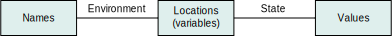
\includegraphics[width=.9\linewidth]{environment_state}
	\end{center}
\end{frame}

\begin{frame}[fragile]{Example of Environment and State}
	\begin{lstlisting}[style=lststyle-c]
	int i;         /* global i */
	...
	void f(...) {
	  int i;       /* local i */
	  ...
	  i = 3;       /* use of local i */
	  ...
	}
	...
	x = i + 1;     /* use of global i */
	\end{lstlisting}
	\vfill
	\begin{center}
	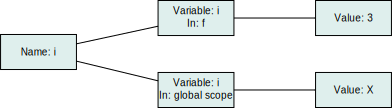
\includegraphics[width=.8\linewidth]{environment_state_example}
	\end{center}
\end{frame}

\subsubsection{Static or dynamic policy}
\begin{frame}{Static or Dynamic Policy}
	\alertbox{One of the most important issues when designing a compiler is related to the decisions the compiler make about the program}
	\vspace{1cm}
	\begin{definitionblock}{Static Policy}
	A program uses a policy that enables the compiler to decide an issue; \emph{the decision could be decided at compile time.}
	\end{definitionblock}
	\vspace{.5cm}
	\begin{definitionblock}{Dynamic Policy}
	The decision can be made when we execute the program; \emph{the decision is required at run time.}
	\end{definitionblock}
\end{frame}

\sidecite{Church.1941, Frege.1967, Wexelblat.1981}
\begin{frame}{Example: Declaration Scope}
	\begin{definitionblock}{Static Scope}
		A language uses a static scope if it is possible to determine the scope of a declaration by looking only at the program (C, Java\dots)
	\end{definitionblock}
	\vspace{1cm}
	\begin{definitionblock}{Dynamic Scope}
		With dynamic scope, as the program runs, the same use of a variable x could refer to any of several different declarations of x (Perl, PHP\dots)
	\end{definitionblock}
\end{frame}

\begin{frame}[background=6]{{``static'' Term Use} in Java}
	\begin{center}
		\code{public static int x = 1;}
	\end{center}
	\vfill
	\begin{itemize}
	\item Here \code{static} refers not to the scope of the variable, but rather to the ability of the compiler to determine the location in memory
	\vfill
	\item If \code{static} is omitted each object has this variable and the compiler cannot determine where it is in advance
	\end{itemize}
\end{frame}

\begin{frame}{{}{Are Environment and State Mappings Dynamic or Static?}}
	\alertbox*{Environment and state mappings are often dynamic}
	\vspace{.5cm}
	\begin{block}{Static or Dynamic Environment Mapping?}
	\begin{itemize}
	\item Most of binding names to locations are \emph{dynamic}
	\item Some declarations (e.g., global \id{i}) are determine at compile time; they are static
	\end{itemize}
	\end{block}
	\vspace{.5cm}
	\begin{block}{Static or Dynamic State Mapping?}
	\begin{itemize}
	\item Most of binding locations to values are \emph{dynamic} because it is impossible to determine the location until we run the program
	\item Declared constants are an exception
	\end{itemize}
	\end{block}
\end{frame}

\subsubsection{Parameter-passing mechanisms}

\begin{frame}{{Parameter-passing} Mechanisms}
	\alertbox*{All programming languages have the notion of procedur; but they can differ in how these procedures get their arguments}
	\vspace{1cm}
	\alertbox{How are the actual parameters (the parameters used in the call of a procedure) associated with the formal parameters (those used in the procedure definition)?}
	\vspace{1cm}
	\begin{columns}
		\begin{column}{.33\linewidth}
			\simplebox{\textcircled{1} Call-by-value}
		\end{column}
		\begin{column}{.33\linewidth}
			\simplebox{\textcircled{2} Call-by-reference}
		\end{column}
		\begin{column}{.33\linewidth}
			\simplebox{\textcircled{3} Call-by-name}
		\end{column}
	\end{columns}
\end{frame}

\begin{frame}[t]{\textcircled{1} Call-by-value}
	\begin{block}{Principle}
		\begin{itemize}
		\item Actual parameter is evaluated or copied
		\item Value is in the location of the formal parameter
		\end{itemize}
	\end{block}
	\begin{block}{Constraints}
		\begin{itemize}
			\item Changes to formal parameter is local to the procedure
			\item Actual parameters themselves cannot be changed
		\end{itemize}
	\end{block}
	\begin{example}
		Used in C and Java; and the default option in C++
	\end{example}
	\begin{alertblock}{Caution}
		In Java, all the object variables are references (or pointers) to the objects. Parameters are passed with the call-by-value policy, not the call-by-reference
	\end{alertblock}
\end{frame}

\begin{frame}{\textcircled{2} Call-by-reference}
	\begin{block}{Principle}
		\begin{itemize}
			\item Address of the actual parameter is passed to the callee as the value of the corresponding formal parameter
			\item Uses of the formal parameter are implemented by following the pointer to the location indicated by the caller
		\end{itemize}
	\end{block}
	\begin{block}{Constraints}
		\begin{itemize}
			\item Changes to the formal parameter thus appear as changes to the actual parameter
		\end{itemize}
	\end{block}
\end{frame}

\begin{frame}{\textcircled{3} Call-by-name}
	\begin{block}{Principle}
		\begin{itemize}
			\item It requires that the callee execute as if the actual parameter were substituted literally for the formal parameter in the code of the callee
			\item Uses of the formal parameter are implemented by following the pointer to the location indicated by the caller
		\end{itemize}
	\end{block}
	\vspace{1cm}
	\begin{example}
		Macro-functions in the C-family languages use this parameter passing mechanism
	\end{example}
\end{frame}


\section[Language processor]{What is a language processor?}

\sectiontableofcontentslide

\begin{frame}{{What is a} Compiler?}
	\begin{itemize}
	\item Read a program in one language --- the source language
	\item Translate it into an equivalent program in a \Emph{low-level language} --- the target language
	\vfill
	\item Report any errors in the source program that are detected during the translation process
	\end{itemize}
	\vfill
	\begin{center}
		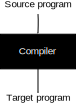
\includegraphics[width=.2\linewidth]{compiler_processor}
	\end{center}
\end{frame}

\begin{frame}{{What is a} Transpiler?}
	\begin{itemize}
		\item Read a program in one language --- the source language
		\item Translate it into an equivalent program in \Emph{another language that is not low-level} --- the target language
		\vfill
		\item Report any errors in the source program that are detected during the translation process
	\end{itemize}
	\vfill
	\begin{center}
		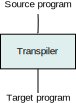
\includegraphics[width=.2\linewidth]{transpiler_processor}
	\end{center}
\end{frame}

\begin{frame}{Running the program}
	If the target program is an executable machine-language program, it can then be called by the user to process inputs and produce outputs
	\vfill
	\begin{center}
		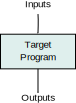
\includegraphics[width=.2\linewidth]{run_program}
	\end{center}
\end{frame}

\begin{frame}{{What is an} Interpreter?}
	\begin{itemize}
	\item A kind of language processor
	\item Does not produce a target program
	\item Directly execute the operations specified in the source program on inputs supplied by the user
	\end{itemize}
	\vfill
	\begin{center}
		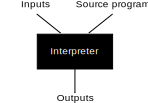
\includegraphics[width=.4\linewidth]{interpreter_processor}
	\end{center}
\end{frame}

\begin{frame}{{What is an} Hybrid Compiler?}
	\begin{itemize}
	\item Combine compilation and interpretation
	\item Generate intermediate program in a platform-independent language
	\item Execute the intermediate program in a platform-dependent virtual machine
	\end{itemize}
	\vfill
	\begin{center}
		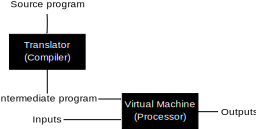
\includegraphics[width=.7\linewidth]{hybrid_processor}
	\end{center}
\end{frame}

\begin{frame}{Properties of the Language Processors}
	\begin{smaller}
	\begin{block}{Compiler v.s. Transpiler v.s. Interpreter}
	\begin{itemize}
	\item Compiler and transpiler is faster than interpreter at mapping inputs to outputs
	\item Interpreter gives better error diagnostics than compiler, because it execute the source program statement by statement (no code optimization)
	\end{itemize}
	\end{block}
	\vspace{1cm}
	\begin{block}{Hybrid Compiler}
	\begin{itemize}
	\item Compile on \emph{one machine}, execute the generated program on \emph{another machine}
	\item To be faster, use just-in-time compilers to translate intermediate programs into machine language and avoid the interpretation, e.g., the Oracle's Java Runtime Environment
	\end{itemize}
	\end{block}
	\end{smaller}
\end{frame}

\begin{frame}<1>[t]{Toolchain}
	\begin{itemize}
	\item Several other programs may be required to create an executable target program
	\item They compose the toolchain of the compiler
	\end{itemize}
	\putat(40,-150){\includeanimatedfigure[width=.8\linewidth]{toolchain}}
\end{frame}

\begin{frame}<2>[t]{Preprocessor in the Toolchain}
	\begin{smaller}
	\begin{block}{\smaller Goals}
	\begin{itemize}
	\item To collect the different files of the program's modules to compile
	\item To expand shorthands, macros into statements
	\end{itemize}
	\end{block}
	\end{smaller}
	\putat(40,-150){\includeanimatedfigure[width=.8\linewidth]{toolchain}}
\end{frame}

\begin{frame}<3>[t]{Compiler in the Toolchain}
	\begin{smaller}
	\begin{block}{\smaller Goals}
	\begin{itemize}
	\item To produce an assembly-language program from the modified source program
	\item Assembly-language is easier to produce and debug
	\end{itemize}
	\end{block}
	\end{smaller}
	\putat(40,-150){\includeanimatedfigure[width=.8\linewidth]{toolchain}}
\end{frame}

\begin{frame}<4>[t]{Assembler in the Toolchain}
	\begin{smaller}
	\begin{block}{\smaller Goals}
	\begin{itemize}
	\item To translate to a machine code that could be relocated in the code segment of the program
	\item Code segment: the part of the memory where machine code is store
	\end{itemize}
	\end{block}
	\end{smaller}
	\putat(40,-150){\includeanimatedfigure[width=.8\linewidth]{toolchain}}
\end{frame}

\begin{frame}<5>[t]{Linker in the Toolchain}
	\begin{smaller}
	\begin{block}{\smaller Goals}
	\begin{itemize}
	\item To resolve external memory addresses, where the code in one file (library or object) may refer to a location in another file (library or object)
	\end{itemize}
	\end{block}
	\end{smaller}
	\putat(40,-150){\includeanimatedfigure[width=.8\linewidth]{toolchain}}
\end{frame}

\section{Process of a compiler}

\sectiontableofcontentslide

\begin{frame}<9>{Process of a Compiler}
	\putat*(340,-197){\includeanimatedfigure[width=2.5cm]{compiler_structure}}
	\begin{minipage}{.8\linewidth}
	\begin{block}{Analysis}
	\begin{itemize}
	\item The \emph{analysis} breaks up the source program into constituent pieces and imposes a grammatical structure to them.
	\item It detects if the source program is ill formed or semantically unsound.
	\item It collects informations about the source program and stores it in a data structure called symbol table.
	\item This part is often called the \emph{front end of the compiler}.
	\end{itemize}
	\end{block}
	\end{minipage}
\end{frame}

\begin{frame}<10>{Process of a Compiler}
	\putat*(340,-197){\includeanimatedfigure[width=2.5cm]{compiler_structure}}
	\begin{minipage}{.8\linewidth}
	\begin{block}{Synthesis}
	\begin{itemize}
	\item The \emph{synthesis} constructs the desired target program from the intermediate representation and the information in the symbol table.
	\item This part is often called the \emph{back end of the compiler}.
	\end{itemize}
	\end{block}
	\end{minipage}
\end{frame}

\begin{frame}<2>{{Lexical Analysis} or Scanning}
	\putat*(340,-197){\includeanimatedfigure[width=2.5cm]{compiler_structure}}
	\begin{minipage}{.8\linewidth}
	\begin{itemize}
	\item Reads the stream of characters making up the source program
	\item Groups the characters into meaningful sequences called \emph{lexemes}
	\item Output for each lexeme:
		\begin{center}
			\ccode{token={\textless}token-name, attribute-value{\textgreater}}
		\end{center}
		\begin{itemize}
		\item \code{token-name}: the identifier of the token
		\item \code{attribute-value}: entry in the symbol table for this token
		\end{itemize}
		\end{itemize}
	\end{minipage}
\end{frame}

\begin{frame}<2>{Example of Scanning}
	\putat*(340,-197){\includeanimatedfigure[width=2.5cm]{compiler_structure}}
	\begin{small}
	\begin{minipage}{.8\linewidth}
	\begin{center}
		\code{position = initial + rate * 60}
	\end{center}
	\begin{tabularx}{\linewidth}{|l|X|}
		\hline
		\tabularheading\chead{Lexeme}&\chead{Token} \\
		\hline
		\code{position} & \ccode{{\textless}id,1{\textgreater}} 
			\begin{itemize}
				\item \ccode{id}: abstract symbol standing for ``identifier''
				\item ``\ccode{1}'': points to the symbol-table entry for position
			\end{itemize} \\
		\hline
		\code{=} & \ccode{{\textless}={\textgreater}} \\
		\hline
		\code{initial} & \ccode{{\textless}id,2{\textgreater}} \\
		\hline
		\code{+} & \ccode{{\textless}+{\textgreater}} \\
		\hline
		\code{rate} & \ccode{{\textless}id,3{\textgreater}} \\
		\hline
		\code{*} & \ccode{{\textless}*{\textgreater}} \\
		\hline
		\code{60} & \ccode{{\textless}number,60{\textgreater}} \\
		\hline
	\end{tabularx}
	\end{minipage}
	\end{small}
\end{frame}

\begin{frame}<2>{Example of Scanning}
	\putat*(340,-197){\includeanimatedfigure[width=2.5cm]{compiler_structure}}
	\putat(0,-120){\includeanimatedfigure[width=.65\linewidth]{compiler_cycle_example}}
\end{frame}

\begin{frame}{Symbol Table}
	\begin{definitionblock}{Symbol Table}
		Central data structure containing a record for each variable name, with record fields for the attributes associated to the name
	\end{definitionblock}
	\vspace{.5cm}
	\begin{definitionblock}{Record Attribute}
		Information about the storage allocated for a name: type, scope, number and types of the formal parameters, the method of passing each argument, and the type of the returned value
	\end{definitionblock}
	\vspace{.5cm}
	\begin{alertblock}{Caution}
		Should be designed to allow the compiler to find the record for each name quickly and to store or retrieve data from that record quickly
	\end{alertblock}
\end{frame}

\begin{frame}{Symbol Table and Scope}
	\alertbox*{Scopes are implemented by setting up a separate symbol table for each scope}
	\vspace{.25cm}
	\begin{block}{Principle}
		The \emph{most-closely nested rule for blocks} permits to define a data structure, which is based on \emph{chained symbol tables}.
	\end{block}
	\begin{center}
		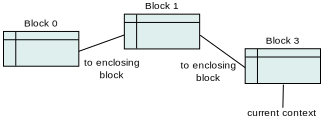
\includegraphics[width=.8\linewidth]{symbol_table_chain}
	\end{center}
\end{frame}

\begin{frame}[t,fragile]{{Simple Java Implementation} of the Symbol Table Chain}
	\begin{lstlisting}[style=lststyle-java]
/** Define the properties of a single symbol. */
public class Symbol {
 public final String lexeme;
 public Type type;
 public Address storagePosition;
 public Symbol(String lexeme) { this.lexeme = lexeme; }
}

/** Define a symbol table. */
public class SymbolTable {

 /** Collection of the symbol in the current context. */
 private final Map<String,Symbol> table = new TreeMap<String,Symbol>();

 /** Reference to the symbol table that is associated to the enclosing scope. */
 private final SymbolTable enclosingEnvironment;

 /** Constructor. */
 private SymbolTable(SymbolTable enclosingEnvironment) {
     this.enclosingEnvironment = enclosingEnvironment;
 }
 //....
	\end{lstlisting}
\end{frame}

\begin{frame}[t,fragile]{{Simple Java Implementation} of the Symbol Table Chain}
	\begin{lstlisting}[style=lststyle-java]
 /** Declare a symbol in the current context. */
 public void declare(String identifier, Symbol symbol) {
     this.table.put(identifier, symbol);
 }

 /** Get the definition of a symbol in the current context,
     or in an enclosing scope. */
 public Symbol get(String identifier) {
     SymbolTable e = this;
     Symbol symbol;
     while (e!=null) {
         symbol = e.table.get(identifier);
         if (symbol != null) {
             return symbol;
         }
         e = e.enclosingEnvironment;
     }
     return null;
 }
 //....
	\end{lstlisting}
\end{frame}

\begin{frame}[t,fragile]{{Simple Java Implementation} of the Symbol Table Chain}
	\begin{lstlisting}[style=lststyle-java]
 /** Reference to the current symbol table.
     The reference is initialized with the
     root context (or the global context). */
 private static SymbolTable current = new SymbolTable(null);

 /** Replies the symbol table of the current context. */
 public static SymbolTable getCurrent() {
     return current;
 }

 /** Open a new context and create the corresponding
     symbol table. */
 public static void openContext() {
     current = new SymbolTable(current);
 }
 /** Close the current context. */
 public static void closeContext() {
     if (current.enclosingEnvironment!=null) {
         current = current.enclosingEnvironment;
     }
 }
}
	\end{lstlisting}
\end{frame}

\begin{frame}<3>{Syntax Analysis}
	\putat*(340,-197){\includeanimatedfigure[width=2.5cm]{compiler_structure}}
	\begin{minipage}{.8\linewidth}
		\alertbox*{Uses the tokens produced by the lexical analyzer to create an intermediate representation}
		\vspace{.5cm}
		\begin{block}{Syntax Tree}
			A typical representation is a syntax tree: \begin{description}
			\item[node] operation in the program
			\item[children] parameters of the operation
			\end{description}
			\vspace{1em}
			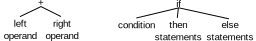
\includegraphics[width=\linewidth]{syntax_tree_example}
		\end{block}
	\end{minipage}
\end{frame}

\begin{frame}<3>{Example of Syntax Analysis}
	\putat*(340,-197){\includeanimatedfigure[width=2.5cm]{compiler_structure}}
	\putat(0,-120){\includeanimatedfigure[width=.65\linewidth]{compiler_cycle_example}}
\end{frame}

\begin{frame}<4>{Semantic Analysis}
	\putat*(340,-197){\includeanimatedfigure[width=2.5cm]{compiler_structure}}
	\begin{minipage}{.8\linewidth}
		\alertbox*{Uses the syntax tree and the information in the symbol table to check the source program for semantic consistency with the language definition}
		\vspace{.25cm}
		\begin{block}{Actions}
			\begin{itemize}
			\item Gathers type information and saves it in either the syntax tree and the symbol table
			\item Applies \emph{coercions}, or type conversions
			\end{itemize}
		\end{block}
		\vspace{.25cm}
		\begin{alertblock}{Type Checking}
			Important part of the semantic analyzer: the compiler checks that each operator has matching operands
		\end{alertblock}
	\end{minipage}
\end{frame}

\begin{frame}<4>{Example of Semantic Analysis}
	\putat*(340,-197){\includeanimatedfigure[width=2.5cm]{compiler_structure}}
	\putat(0,-120){\includeanimatedfigure[width=.65\linewidth]{compiler_cycle_example}}
\end{frame}

\begin{frame}<5>{{Intermediate Code} Generator}
	\putat*(340,-197){\includeanimatedfigure[width=2.5cm]{compiler_structure}}
	\begin{minipage}{.8\linewidth}
		\alertbox*{Many compilers generate an \emph{explicit low-level or machine-like intermediate representation}, which is a program for an abstract machine}
		\vspace{1cm}
		\begin{block}{Intermediate code}
			Two representations are generally used: \begin{itemize}
				\item Syntax tree
				\item Three-address code
			\end{itemize}
			that is easy to produce, and translate into the target machine
		\end{block}
	\end{minipage}
\end{frame}

\begin{frame}{{What is} Three-address Code?}
	\alertbox*{A sequence of assembly-like instructions with, at most, three operands per instruction. \\
		\ccode{{\textless}variable{\textgreater} = {\textless}operand1{\textgreater} {\textless}operator{\textgreater} {\textless}operand2{\textgreater}}}
	\begin{itemize}
	\item Each operand can act like a register
	\item The affectation operator is implicit and always present
	\end{itemize}
	\begin{alertblock}{Constraints}
		\begin{enumerate}
			\item At most one operator on the right side
			\item Temporary names are generated to hold the value computed by the three-address instruction
			\item Some instructions have fewer then three operands
		\end{enumerate}
	\end{alertblock}
\end{frame}

\begin{frame}<5>{Example of Intermediate Code Generation}
	\putat*(340,-197){\includeanimatedfigure[width=2.5cm]{compiler_structure}}
	\putat(0,-120){\includeanimatedfigure[width=.65\linewidth]{compiler_cycle_example}}
\end{frame}

\begin{frame}<6>{{Machine-Independent Code} Optimizer}
	\putat*(340,-197){\includeanimatedfigure[width=2.5cm]{compiler_structure}}
	\begin{minipage}{.8\linewidth}
		\alertbox*{Improves the intermediate code for better target code \\
			(faster, shorter, less power consumer\dots)}
		\vspace{.5cm}
		\begin{itemize}
		\item All the compilers include a machine-independent code optimizer
		\item Those that spent a large amount of time on this phase are named ``optimizing compilers''
		\end{itemize}
		\vspace{.5cm}
		\begin{block}{Note}
			Many of the simple optimizations permit to significantly improve the running time of the target program without too much time spent on this phase
		\end{block}
	\end{minipage}
\end{frame}

\figureslide{Example of Optimization}{intermediate_code_optim}

\begin{frame}<6>{Example of Machine-Independent Code Optimization}
	\putat*(340,-197){\includeanimatedfigure[width=2.5cm]{compiler_structure}}
	\putat(0,-120){\includeanimatedfigure[width=.65\linewidth]{compiler_cycle_example}}
\end{frame}

\begin{frame}<7>{Code Generator}
	\putat*(340,-197){\includeanimatedfigure[width=2.5cm]{compiler_structure}}
	\begin{minipage}{.8\linewidth}
		\alertbox*{Maps an intermediate representation into the target language}
		\vspace{.5cm}
		\begin{itemize}
		\item If the target language is machine code, registers or memory locations are selected for each variables used by the program
		\item Then, the intermediate instructions are translated into sequences of machine instructions that perform the same tasks
		\vspace{.5cm}
		\item A crucial aspect is the judicious assignment of registers to hold variables
		\end{itemize}
	\end{minipage}
\end{frame}

\begin{frame}{Example of Code Generation}
	\begin{itemize}
	\item Assumes that R1 and R2 are registers
	\item Variables are mapped to registers so that they can be easily used for the generation of the next instructions
	\end{itemize}
	\vspace{.25cm}
	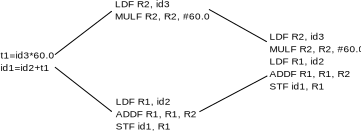
\includegraphics[width=\linewidth]{code_generator_example}
\end{frame}

\begin{frame}<7>{Example of Code Generation}
	\putat*(340,-197){\includeanimatedfigure[width=2.5cm]{compiler_structure}}
	\putat(0,-120){\includeanimatedfigure[width=.65\linewidth]{compiler_cycle_example}}
\end{frame}

\section{Tools to create a compiler}
\sectiontableofcontentslide

\begin{frame}{Tools to Create a Compiler}
	\alertbox*{Several tools are available to help the compiler writer to build his compiler}
	\vspace{.5cm}
	\fancybox{Scanner generators}{Lexical analyzers from a reg-ex description tokens \\
	(Flex, JFlex\dots)}{scanner-icon}{1}
	\hfill
	\fancybox{Parser generators}{Syntax analyzers from grammar \\
	(Yacc, JavaCC, Bison\dots)}{parser-icon}{2}
	\hfill
	\fancybox{Syntax-directed translation engines}{Parse-tree walkthrough routines for intermediate code generation}{assembly-icon}{3}
\end{frame}

\begin{frame}{Tools to Create a Compiler \insertcontinuationtext}
	\fancybox{Code-generator generators}{Procedures for generating target machine code from intermediate code}{machine-code-icon}{4}
	\hfill
	\fancybox{Data-flow analysis engines}{Help for management of value exchange between compiler components}{data-flow-icon}{5}
	\hfill
	\fancybox{Construction toolkits}{Include the other tools and IDE integration (Xtext\dots)}{toolkit-icon}{6}
\end{frame}

\section{Conclusion}
\sectiontableofcontentslide

\begin{frame}[t]{{Key Concepts} in the Chapter}
	\begin{description}
	\item[Language Processors] An integrated software development environment: compilers, interpreters, linkers, loaders, debuggers, profilers.
	\item[Compiler Phases] Sequence of phases, each of which transforms the source program from one intermediate representation to another.
	\item[Machine and Assembly Languages] Machine languages were the first-generation programming languages, followed by assembly languages.
	\item[Code Optimization] the science of improving the efficiency of code in both complex and very important. It is a major portion of the study of compilation.
	\item[Higher-Level Languages] Programming languages take on progressively more of the tasks that formerly were left to the programmer: memory management, type-consistency\dots
	\item[Environments] The association of names with locations in memory and then with values can be described in terms of environments.
	\item[Parameter Passing] Parameters are passed from a calling procedure to the callee either by value or by reference.
	\end{description}
\end{frame}

\begin{frame}[t]{{Key Concepts} in the Chapter \insertcontinuationtext}
	\begin{description}
		\item[Aliasing] When parameters are (effectively) passed by reference, two formal parameters can refer to the same object.
		\item[Compiler Front End] The part of the compiler that is dedicated to the analysis phases. The compiler front end takes the source program, breaks it to token, analyzes the grammar, detects errors and inconsistencies, and generate an intermediate representation.
		\item[Compiler Back End] The part of the compiler that is dedicated to the synthesis phases. The compiler back end takes the intermediate representation, generates assembly and machine code.
		\item[Lexical Analyzer] The lexical analyzer reads the input one character at a time and produces as output a stream of tokens. A token consists of a terminal symbol and attribute values.
		\item[Parsing] Parsing is the problem of figuring out how a string of terminals can be derived from the start symbol of the grammar by repeatedly replacing a nonterminal by the body of one of its productions.
	\end{description}
\end{frame}


\begin{frame}[t]{{Key Concepts} in the Chapter \insertcontinuationtext}
	\begin{description}
		\item[Parse Tree] A graphical tree representation of the productions that are matching a sequence of input tokens.
		\item[Intermediate Code] The result of the syntax analysis is a representation of the source program, called intermediate code. Two primary forms of intermediate code are illustrated: abstract syntax tree (similar to parse tree), and three-address code.
		\item[Symbol Table] A data structure that holds information about identifiers.
	\end{description}
\end{frame}

%allowframebreaks
\begin{frame}[t,fancyframetitle=false]{{\bibname} of the Chapter}%
	\tiny%
	\putbib[chapters/chapter1/biblio]%
\end{frame}%

\end{bibunit}
\end{graphicspathcontext}

%\part[author={\protect\insertauthor},label={chap:lexical_analysis}]{Lexical Analysis}

\begin{graphicspathcontext}{{./chapters/chapter1/imgs/auto/},{./chapters/chapter2/imgs/auto/},{./chapters/chapter2/imgs/raw/}}
\begin{bibunit}[apalike]
	
\tableofcontentslide

\section{Introduction}
\sectiontableofcontentslide

\subsection{General principles}

\begin{rightlawnframe}<2>{Lexical Analyser}{lexical-analyzer-introduction}
	\putat*(340,-197){\includeanimatedfigure[width=2.5cm]{compiler_structure}}
	The lexical analyzer reads source program and extract lexemes \\[1cm]
	Each lexeme is associated to a token: \\
	\ccode{{\textless}token-name, \\
	\ attribute-value{\textgreater}} \\[1cm]
	Outputs the tokens
\end{rightlawnframe}

\begin{frame}{{Process of the} Lexical Analyzer}
	\begin{columns}
		\begin{column}{.5\linewidth}
			\begin{rightanchorblock}{}{1}
				Discovering the tokens
			\end{rightanchorblock}
			\begin{rightanchorblock}{}{2}
				Stripping the blanks and the comments
			\end{rightanchorblock}
			\begin{rightanchorblock}{}{3}
				Correlating the error messages with the source program (line number tracking\dots)
			\end{rightanchorblock}
		\end{column}
		\begin{column}{.5\linewidth}
			\begin{block}{Cascading Process (most of the time)}
				\begin{enumerate}
					\item[Scanning] processes that do not require tokenization of the input, e.g. deletion of comments and compaction of consecutive white spaces
					\item[Lexical analysing] produces tokens from the output of the scanner
				\end{enumerate}
			\end{block}
		\end{column}
	\end{columns}
\end{frame}

\subsection{Definitions}
\subsectiontableofcontentslide

\begin{frame}{Lexeme}
	\begin{definition}
		A sequence of characters in the source program that is identified by the lexical analyzer as a lexical unit (element of the language)
	\end{definition}
	\vspace{1cm}
	\begin{example}
		\begin{itemize}
		\item Let the statement: \code{printf("Total = \%d\n", score);}
		\item Both \code{printf} and \code{score} are lexemes
		\item String of characters is a lexeme
		\item Parenthesis, coma and semicolumn characters are also lexemes
		\end{itemize}
	\end{example}
\end{frame}

\begin{frame}{Token}
	\begin{definition}
		A pair consisting of a token \emph{name} and an optional \emph{attribute value}
		\begin{itemize}
			\item name: abstract symbol representing a kind of lexical unit
			\item token names are the input symbols that the parser processes
			\item token name is written in \token{bold-face}
		\end{itemize}
	\end{definition}
	\vfill
	\begin{example}
		\begin{itemize}
		\item Let the statement: \code{printf("Total = \%d\n", score);}
		\item both \code{printf} and \code{score} are lexemes matching the pattern for token \token{id}
		\end{itemize}
	\end{example}
\end{frame}

\begin{frame}{Pattern}
	\begin{definition}
		A description of the form that the lexemes of a token may take
		\begin{itemize}
			\item For keyword: the pattern is a sequence of characters that form the keyword
			\item For identifier and some other token: the pattern is a more complex structure that is \emph{matched} by many strings
		\end{itemize}
	\end{definition}
	\vspace{1cm}
	\begin{example}
		\begin{itemize}
		\item Let the statement: \code{printf("Total = \%d\n", score);}
		\item both \id{printf} and \id{score} are described by the pattern \regex{[\_a-zA-Z][\_a-zA-Z]*} (regex)
		\end{itemize}
	\end{example}
\end{frame}

\begin{frame}{Classes of Tokens}
	In many programming languages, the following classes cover most or all of the tokens: \\[.5cm]
	\begin{tabularx}{\linewidth}{|l|X|}
		\hline
		\tabularheading\chead{Class} & \chead{Description} \\
		\hline
		\token{keyword} & Pattern is the name of the token itself \\
		\hline
		\token{operator} & Individually or in classes, e.g., class \token{comparison} \\
		\hline
		\token{identifier} & One token per identifier \\
		\hline
		\token{constant} & One token per type of constant, e.g. number or string literal \\
		\hline
		\token{punctuation} & One token per punctuation symbol, e.g. left and right parentheses, comma, and semicolon \\
		\hline
	\end{tabularx}
\end{frame}

\begin{frame}{Attribute of Token}
	\begin{definition}
		Additional information associated to a token, when more than one lexeme can match a pattern
	\end{definition}
	\vspace{.5cm}
	\begin{examples}
		\begin{itemize}
		\item value of the parsed number (lexeme) for token \token{number}
		\item position of the identifier into the symbol table for token \token{id}
		\end{itemize}
	\end{examples}
	\vspace{.5cm}
	\begin{alertblock}{Assumption}
		Usually, token has at most one associated attribute; but it could be a data structure
	\end{alertblock}
\end{frame}

\subsection{Separating the lexical analyzer and the parser}
\subsectiontableofcontentslide

\begin{frame}{Relation between the Lexical Analyzer and the Parser}
	\alertbox*{Lexical analyzer generally does not control the execution flow of the compiler}
	\vspace{.5cm}
	\begin{center}
		\pgfuseimage{lexical-parser-relation}
	\end{center}
	\vspace{.5cm}
	\begin{itemize}
	\item Lexical analyzer is invoked by the parser through a call to \code{getNextToken} function
	\item Then, lexical analyzer tries to discover and to reply a token
	\end{itemize}
\end{frame}

\begin{frame}{{Why Separating} Lexical Analyzer and Parser?}
	\fancybox{Design Simplicity}{Enable simplification of at least one of these tasks}{software-design}{1}
	\hfill
	\fancybox{Compiler Efficiency}{Enable application of specialized techniques}{software-efficiency}{2}
	\hfill
	\fancybox{Easier Portability}{Specific input devices supported by lexical analyzer}{software-portability}{3}
\end{frame}

\subsection{Lexical errors}
\subsectiontableofcontentslide

\begin{frame}[t]{Lexical Errors}
	\alertbox{It is hard for a lexical analyzer to tell that there is a source-code error}
	\vspace{.25cm}
	\begin{example}
		\code{fi ( a == f(x) ) ...}
	\end{example}
	\vspace{.25cm}
	\begin{alertblock}{Problems}
		\begin{itemize}
		\item Cannot tell whether \code{fi} is a misspelling of the keyword \code{if} or an undeclared function identifier
		\item Fails when none of the patterns for tokens matches any prefix of the remaining input
		\end{itemize}
	\end{alertblock}
	\vspace{.25cm}
	\alertbox*{If such an error is detected, lexical analyzer must output an error message \\
		and try to \emph{recover} a stable state}
\end{frame}

\begin{leftlawnframe}{{Recovery Strategy:} Panic Mode}{panic-mode}
	Successive characters are deleted from the remaining input, until the lexical analyzer can find a well-formed token at the beginning of input
\end{leftlawnframe}

\begin{gridframe}{{Other} Recovery Strategies}
	\cell2{delete-icon}{\small Delete character from input}
	\cell4{insert-icon}{\small Insert character into input}
	\cell7{replace-icon}{\small Replace character in input}
	\cell9{transpose-icon}{\small Transpose adjacent characters}
\end{gridframe}

\section{Input buffering}
\sectiontableofcontentslide

\begin{frame}{Reading the Source Program}
	\begin{rightarrowsequence}
		\arrow[decoration=icon-goal]{Reading input is key task that must be efficient}
		\arrow[bg=CIADmagenta, decoration=icon-problem]{Have to look one or more characters beyond the next lexeme to extract the right lexeme}
		\arrow[bg=CIADgreen, decoration=icon-solution]{Two-buffer scheme that handles large lookaheads safely}
	\end{rightarrowsequence}
	\vspace{.25cm}
	\begin{example}
		To be sure that a character is the last of an identifier, the next character must be read, and it is not part of the lexeme for \token{id}
	\end{example}
\end{frame}

\begin{frame}{Principles of the Two-Buffer Scheme}
	\alertbox*{Two buffers are read and used alternatively}
	\begin{center}
		{\pgfuseimage{buffer_pair_example}}
	\end{center}
	\vspace{.25cm}
	\begin{description}
		\item[Assumption] the larger lexeme has a size lower or equals to $N$
		\item $N$ is usually the size of the disk block
		\item \token{eof} character is put in the buffer when there is not enough characters in the input
	\end{description}
	\vspace{1cm}
	\simplebox{\Emph{How to be efficient?} By invoking the \code{read} system function for $N$ characters rather than a call per character}
\end{frame}

\begin{frame}[t]{{Two Reading} Pointers}
	\begin{center}
		{\pgfuseimage{buffer_pair_example1}}
	\end{center}
	\begin{itemize}
	\item \id{lexemeBegin}: the beginning of the current lexeme
	\item \id{forward}: the current character
	\end{itemize}
	\vspace{.25cm}
	\begin{block}{Algorithmic Principle}
		\begin{enumerate}
			\item \emph{If \id{forward} is outside a buffer}, the other buffer is reloaded from the input, and move \id{forward} to the beginning of the newly loaded buffer
			\item \emph{If character pointed by \id{forward} does not match a lexeme from \id{lexemeBegin}}:
				\begin{itemize}
					\item \emph{If is is a valid lexeme}, output the lexeme, move \id{lexemeBegin} to \id{foward}
					\item \emph{Else} generate an error
				\end{itemize}
			\item \emph{Else} move \id{forward} to the right
		\end{enumerate}
	\end{block}
\end{frame}

\begin{frame}{{Be More Efficient} with Sentinels}
	\begin{alertblock}{Problem of efficiency}
		For each character read, two tests: \begin{enumerate}
		\item one for the end of the buffer
		\item one to determine what character is read (usually with a multiway branch)
		\end{enumerate}
	\end{alertblock}
	\vspace{.5cm}
	$\Rightarrow$ To improve the speed of the treatment, we can combine the two tests by extending each buffer with a \emph{sentinel character} (usually \token{eof}) \\
	\vspace{.5cm}
	\begin{center}
		\pgfuseimage{buffer_pair_sentinel_example}
	\end{center}
\end{frame}

\begin{frame}{{Can We Run Out Of} Buffer Space?}
	\begin{rightarrowsequence}
		\arrow{
			In most modern languages, lexemes are short \\
			$N \ge 1000$ is ample
		}
		\arrow[bg=CIADmagenta, decoration=icon-problem]{
			Character strings can be very long (more than $N$)
		}
		\arrow[bg=CIADgreen, decoration=icon-solution]{
			Add a dynamic buffer scheme for large lexeme
		}
		\arrow[bg=CIADgreen, decoration=icon-solution]{
			Reply a sequence of \token{str} tokens, one for each of the shorter strings (see example)
		}
	\end{rightarrowsequence}
	\begin{example}
		Compile-time string concatenation in C: \code{"ABC" "DEF"}
	\end{example}
\end{frame}


\section[Token Recognition]{Specification and recognition of tokens}
\sectiontableofcontentslide

\subsection{Definitions and operations on languages}
\subsectiontableofcontentslide

\begin{frame}{Definitions of Alphabet, String and Language}
	\begin{definitionblock}{Alphabet}
		Any finite set of symbols; \inlineexample{$A = \left\{a,b,c,\delta\right\}$}
	\end{definitionblock}
	\vspace{.25cm}
	\begin{definitionblock}{String}
		A finite sequence $s$ of symbols drawn from an alphabet $A$. \\
		\inlineexample{$s \in S / S = \permut(\powerset(A)) \setminus \{\emptyset\} = \left\{a,b,c,\delta,ab,ac,a\delta,\dots\right\}$} \\
		$|s|$ is the size of $s$
	\end{definitionblock}
	\vspace{.25cm}
	\begin{definitionblock}{Language}
		Any countable set of strings over some fixed alphabet \\
		\inlineexample{$L \subseteq S = \left\{abc,\delta,b,bc\right\}$}
		%	\end{itemize}
	\end{definitionblock}
\end{frame}

\sidecite{Kleene.1956}
\begin{frame}{Operations on Languages}
	\alertbox*{The following operations are used for defining the pattern matchings for languages}
	\vspace{1cm}
	\begin{block}{Union of the languages $L$ and $M$}
		$L \cup M = \left\{s | s\in L \vee s \in M\right\}$
		\begin{tabularx}{\linewidth}{@{}lX@{}}
		\insertexamplelabel & Let $L = \left\{ a, b ,c \right\}$ and $M = \left\{ d, e \right\}$ \\
		& then $L \cup M = \left\{ a, b, c, d, e \right\}$
		\end{tabularx}
	\end{block}
	\vspace{.5cm}
	\begin{block}{Concatenation of the languages $L$ and $M$}
		$LM = \left\{st | s\in L, t \in M\right\}$
		\begin{tabularx}{\linewidth}{@{}lX@{}}
		\insertexamplelabel & Let $L = \left\{ a, b ,c \right\}$ and $M = \left\{ d, e \right\}$ \\
		& then $LM = \left\{ ad, ae, bd, be, cd, ce \right\}$
		\end{tabularx}
	\end{block}
\end{frame}

\sidecite{Kleene.1956}
\begin{frame}{Operations on Languages \insertcontinuationtext}
	\begin{block}{Self-concatenation of the language $L$}
		$L^i = \begin{cases}
			\{\epsilon\} & \text{if }i=0 \\
			L^{i-1}L & \text{if }i>0 \\
			\end{cases}$
		\begin{tabularx}{\linewidth}{@{}lX@{}}
		\insertexamplelabel & Let $M = \left\{ d, e \right\}$ \\
		& then $M^4 = \left\{ \begin{array}{l}
			\scriptstyle dddd, ddde, ddded, ddee, dedd, dede, \\
			\scriptstyle deded, deee, eddd, edde, edded, edee, \\
			\scriptstyle eedd, eede, eeded, eeee \end{array} \right\}$
		\end{tabularx}
	\end{block}
\end{frame}

\sidecite{Kleene.1956}
\begin{frame}[c]{Operations on Languages \insertcontinuationtext}
	\begin{block}{Kleene's Closure of the language $L$}
		$L^* = \bigcup^{\infty}_{i=0}L^i$
		\begin{tabularx}{\linewidth}{@{}lX@{}}
		\insertexamplelabel & Let $M = \left\{ d, e \right\}$ \\
		& then $M^* = \left\{ \begin{array}{l}
			\scriptstyle \epsilon, d, e, dd, de, ed, ee, ddd, dde, ded, dee, edd, ede, eed, \\
			\scriptstyle eee, dddd, ddde, dded, ddee, dedd, dede, deed, deee, \dots\end{array} \right\}$
		\end{tabularx}
	\end{block}
	\vspace{.5cm}
	\begin{block}{Positive Closure of the language $L$}
		$L^+ = \bigcup^{\infty}_{i=1}L^i$
		\begin{tabularx}{\linewidth}{@{}lX@{}}
		\insertexamplelabel & Let $M = \left\{ d, e \right\}$ \\
		& then $M^+ = \left\{ \begin{array}{l}
			\scriptstyle d, e, dd, de, ed, ee, ddd, dde, ded, dee, edd, ede, eed, \\
			\scriptstyle eee, dddd, ddde, dded, ddee, dedd, dede, deed, \dots\end{array} \right\}$
		\end{tabularx}
	\end{block}
\end{frame}

\subsection{Regular expressions}
\subsectiontableofcontentslide

\sidecite{Kleene.1956, Shannon.1956, Aho.1990, Aho.1988}
\begin{frame}{Regular Expressions}
	\begin{definitionblock}{Regular Expressions (shortened as regex, regexp or rational expression)}
		A sequence of characters that specifies a search pattern.
	\end{definitionblock}
	\vspace{.5cm}
	\begin{rightarrowsequence}
		\arrow{Usually used for describing all the languages that can be built from the operators previously defined}
		\arrow{
			Built recursively out of smaller regular expressions (see following slides). \\[.25cm]
			Each regular expression $r$ denotes a language $L(r)$, which is also defined recursively from the languages denoted by $r$'s expressions.
		}
	\end{rightarrowsequence}
\end{frame}

\begin{frame}{Basis of Regular Expressions}
	The rules that define the regular expressions over some alphabet $\Sigma$ and the languages that those expressions denote are:
	\vspace{.25cm}
	\begin{definition}[BASIS]
	There are two rules that form the basis: \begin{enumerate}
	\item $\epsilon$ is a regular expression, and $L(\epsilon)$ is $\{\epsilon\}$, that is, the language whose sole member is the empty string.
	\item If a is a symbol in $\Sigma$, then \regex{a} is a regular expression, and $L(\regex{a}) = \{a\}$, that is, the language with one string, of length one, with $a$ in its position.
	\end{enumerate}
	\end{definition}
	\vspace{.25cm}
	\begin{block}{\smaller Remark}\smaller 
		By convention, we use \textit{italics} for symbols, and \regex{boldface} for their corresponding regular expressions.
	\end{block}
\end{frame}

\begin{frame}{Induction with Regular Expressions}
	\begin{definition}[INDUCTION]
	There are four parts to the induction whereby larger regular expressions are built from smaller ones. Suppose $r$ and $s$ are regular expressions denoting languages $L(r)$ and $L(s)$, respectively.
	\begin{enumerate}
	\item $(r)|(s)$ is a regular expression denoting the language $L(r) \cup L(s)$
	\item $(r)(s)$ is a regular expression denoting the language $L(r)L(s)$
	\item $(r)*$ is a regular expression denoting the language $(L(r))^*$
	\item $(r)$ is a regular expression denoting $L(r)$
	\end{enumerate}
	\end{definition}
	This last rule says that we can add additional pairs of parentheses around expressions without changing the language they denote.
\end{frame}

\begin{frame}{Simplification Conventions for Induction}
	\alertbox*{Regular expressions often contain unnecessary pairs of parentheses}
	\vspace{1cm}
	\begin{block}{Simplification Rules}
		\begin{enumerate}[a)]
			\item The unary operator "$*$" has highest precedence and is left associative.
			\item Concatenation has second highest precedence and is left associative.
			\item "$|$" has lowest precedence and is left associative.
		\end{enumerate}
	\end{block}
\end{frame}

\begin{frame}{Regular Set}
	\begin{definitionblock}{Regular Set}
		A language that can be defined by a regular expression \\
		\smaller If two regular expressions $r$ and $s$ denote the same regular set, they are equivalent $r = s$
	\end{definitionblock}
	\vspace{.5cm}
	\begin{tabularx}{\linewidth}{|X|X|X|}
		\hline
		\tabularheading\chead{Law}&\chead{Description} \\
		\hline
		$r|s = s|r$ & $|$ is commutative \\
		\hline
		$r|(s|t) = (r|s)|t$ & $|$ is associative \\
		\hline
		$r(st) = (rs)t$ & Concatenation is associative \\
		\hline
		$r(s|t) = rs|rt$; $(s|t)r = st|tr$ & Concatenation distributes over $|$ \\
		\hline
		$\epsilon r = r\epsilon = r$ & $\epsilon$ is the identity for concatenation \\
		\hline
		$r* = (r|\epsilon)*$ & $\epsilon$ is guaranteed in a closure \\
		\hline
		$r** = r*$ & $*$ is idempotent \\
		\hline
	\end{tabularx}
\end{frame}

\subsection{Regular definitions}
\subsectiontableofcontentslide

\begin{frame}[t]{Regular Definitions}
	\alertbox{For notational convenience, we may wish to give names to certain regular expressions and use those names in subsequent expressions, as if the names were themselves symbols}
	\vspace{.25cm}
	\begin{definitionblock}{Regular definition}
		If $\Sigma$ is an alphabet of basic symbols, a regular definition is a sequence of definitions of the form: \\
		\centering\begin{tabular}{rcl}
			\regex{d\textdown{1}} & $\rightarrow$ & $r_1$ \\
			\regex{d\textdown{2}} & $\rightarrow$ & $r2$ \\
			& \dots &\\
			\regex{d\textdown{n}} & $\rightarrow$ & $r_n$ \\
		\end{tabular}
		\begin{itemize}
			\item \regex{d\textdown{i}} is a new symbol, not in and not the same as any other of the $d$'s
			\item $r_i$ is a regular expression over the alphabet $\Sigma\cup\{\regex{d\textdown{1}},\regex{d\textdown{2}},\dots,\regex{d\textdown{i-1}}\}$.
		\end{itemize}
	\end{definitionblock}
\end{frame}

\begin{frame}[background=8]{Well-known Regular Definitions}
	\centering
	\begin{tabular}{rcl}
		\regex{letter} & $\rightarrow$ & $A | B | \dots | Z | a | b | \dots | z$ \\[.2cm]
		\regex{letter\_} & $\rightarrow$ & $\regex{letter} | \_$ \\[.2cm]
		\regex{digit} & $\rightarrow$ & $0 | 1 | \dots | 9$ \\[.2cm]
		\regex{letters} & $\rightarrow$ & $\regex{letter}\ \regex{letter}*$ \\[.2cm]
		\regex{digits} & $\rightarrow$ & $\regex{digit}\ \regex{digit}*$ \\[.2cm]
		\regex{id} & $\rightarrow$ & $\regex{letter\_} ( \regex{letter\_} | \regex{digit} )*$ \\[.2cm]
		\regex{optFrac} & $\rightarrow$ & $.\ \regex{digits} | \epsilon$ \\[.2cm]
		\regex{optExp} & $\rightarrow$ & $( (E|e) (+|-|\epsilon) \regex{digits} ) | \epsilon$ \\[.2cm]
		\regex{number} & $\rightarrow$ & \regex{digits}\ \regex{optFrac}\ \regex{optExp} \\
	\end{tabular}
\end{frame}

\sidecite{Kleene.1956}
\begin{frame}[t]{Extension of the Regular Definitions}
	\alertbox*{Since \cite{Kleene.1956} introduced regular expressions with the basic operators in 1950s, many extensions have been added to enhance their ability to specify string patterns}
	\vspace{.25cm}
	\fancybox{One or more instances}{
		$L(r+) = (L(r))^+$ \\
		Same precedence and associativity as "$*$"}{rplus_regex}{1}
	\hfill
	\fancybox{Zero or one instance}{
		$L(r?) = L(r)\cup\{\epsilon\}$ \\
		Same precedence and associativity as "$*$"}{rquestionmark_regex}{2}
	\hfill
	\fancybox{Character classes}{
		$[ab{\ldots}z] = a|b|\ldots|z$ \\
		Consecutive symbols: $[a-z]$}{class_regex}{3}
\end{frame}

\begin{frame}[background=8]{Revision of the Regular Definitions}
	\centering
	\begin{tabular}{rcl}
		\regex{letter} & $\rightarrow$ & $[A-Za-z]$ \\[.2cm]
		\regex{letter\_} & $\rightarrow$ & $[A-Za-z\_]$ \\[.2cm]
		\regex{digit} & $\rightarrow$ & $[0-9]$ \\[.2cm]
		\regex{letters} & $\rightarrow$ & $\regex{letter}+$ \\[.2cm]
		\regex{digits} & $\rightarrow$ & $\regex{digit}+$ \\[.2cm]
		\regex{id} & $\rightarrow$ & $\regex{letter\_} ( \regex{letter\_} | \regex{digit} )*$ \\[.2cm]
		\regex{number} & $\rightarrow$ & $\regex{digits} (. \regex{digits})? ([Ee][+-]? \regex{digits})?$ \\
	\end{tabular}
	\[\begin{array}{@{}ll@{}}
		
	\end{array}\]
\end{frame}

\subsection{Recognition of tokens}

\subsubsection{Definition of the Lexeme-Token Pairs}
\subsubsectiontableofcontentslide*

\begin{frame}{Definition of our Illustrative Language}
	\alertbox*{We are able to express patterns using regular expressions \\
		How to regex patterns for all the tokens of our language?}
	\vspace{.5cm}
	\centering
	\begin{tabular}{rcl}
		\regex{term} & $\rightarrow$ & \regex{number} \\
		& $\rightarrow$ & \regex{id} \\[.2cm]
		\regex{expr} & $\rightarrow$ & \regex{term} \ccode{=} \regex{term} \\
		& $\rightarrow$ & \regex{term} \ccode{{\textless}{\textgreater}} \regex{term} \\
		& $\rightarrow$ & \regex{term} \ccode{\textless} \regex{term} \\
		& $\rightarrow$ & \regex{term} \ccode{\textgreater} \regex{term} \\
		& $\rightarrow$ & \regex{term} \ccode{\textless=} \regex{term} \\
		& $\rightarrow$ & \regex{term} \ccode{\textgreater=} \regex{term} \\[.2cm]
		\regex{statement} & $\rightarrow$ & \ccode{\kw{if}} \regex{expr} \ccode{\kw{then}} \regex{statement} \ccode{\kw{else}} \regex{statement} \\
		& $\rightarrow$ & \regex{term} \\
	\end{tabular}
\end{frame}

\begin{frame}{Definition of the Lexeme-Token Pairs}
	\begin{small}
	\begin{tabularx}{\linewidth}{|l|X|l|X|}
		\hline
		\tabularheading\chead{Lexeme}&\chead{Regular Expression}&\chead{Token}&\chead{Token Attributes} \\
		\hline
		ws & $[\ {\backslash}n{\backslash}t{\backslash}r]+$ & - & - \\
		\hline
		if & $if$ & \token{if} & - \\
		\hline
		then & $then$ & \token{then} & - \\
		\hline
		else & $else$ & \token{else} & - \\
		\hline
		id & $\regex{letter\_}\ (\regex{letter\_}|\regex{digit})*$ & \token{id} & pointer to symbol table's entry \\
		\hline
		number & $\regex{digits}(.\ \regex{digits})?$ & \token{number} & pointer to symbol table's entry \\
		\hline
		= & $=$ & \token{relop} & \ccode{EQ} \\
		\hline
		{\textless}{\textgreater} & $<>$ & \token{relop} & \ccode{NE} \\
		\hline
		{\textless} & $<$ & \token{relop} & \ccode{LT} \\
		\hline
		{\textgreater} & $>$ & \token{relop} & \ccode{GT} \\
		\hline
		{\textless}= & $<=$ & \token{relop} & \ccode{LE} \\
		\hline
		{\textgreater}= & $>=$ & \token{relop} & \code{GE} \\
		\hline
	\end{tabularx}
	\end{small}
\end{frame}

\subsubsection{Transition Diagram}
\subsubsectiontableofcontentslide

\begin{frame}[t]{Transition Diagram}
	As an intermediate step in the construction of a lexical analyzer, patterns are converted to flowcharts, called \emph{transition diagrams}.
	\vspace{.5cm}
	\begin{definition}[Transition Diagram]
	\begin{description} 
	\item[Diagram] composed of states and edges
	\item[State] a step in the scanning of a string, that also indicates if the input stream is validating the regular expression, or not
	\item[Edge] directed from one state to another. Each edge is labeled by a symbol or a set of symbols
	\end{description}
	\end{definition}
	\begin{alertblock}{Assumption}
	All transition diagrams are deterministic: never more than one edge out of a given state with a given symbol among its labels.
	\end{alertblock}
\end{frame}

\begin{frame}{Specific Notations}
	\begin{small}
		\begin{tabularx}{\linewidth}{|c|X|}
			\hline
			\tabularheading\chead{Notation}&\chead{Explanation} \\
			\hline
			\raisebox{-.7\height}{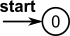
\includegraphics[width=4em]{transition_diagram_start}} &  The transition diagram always begins in the \emph{start state} before any input symbols have been read. \\
			\hline
			\raisebox{-.8\height}{
\includegraphics[width=5em]{transition_diagram_other}} &  The transition labelled with \textbf{other} is traversable when no other transition is traversable. \\
			\hline
			\raisebox{-.7\height}{
\includegraphics[width=1.7em]{transition_diagram_accept_state}} & The \emph{accepting state} (or final) indicates that a lexeme has been found (between pointers \code{lexemeBegin} and \code{forward}).
			\\
			\hline
			\raisebox{-\height}{
\includegraphics[width=2em]{transition_diagram_retract_state}} & If the lexeme does not include the symbol that got us to the accepting state, it is necessary to \emph{retract} the \code{forward} pointer by one position. \\
			\hline
		\end{tabularx}
	\end{small}
\end{frame}

\figureslide{Example of a Transition Diagram for \token{relop}}{transition_diagram_relop}

\begin{frame}{Problem with Identifiers and Keywords}
	\begin{itemize}
	\item The transition diagram that recognizes the identifiers is:
	\vfill
		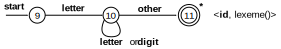
\includegraphics[width=\linewidth]{transition_diagram_identifier}
	\vfill
	\item \code{lexeme()} replies the current lexeme (between \code{lexemeBegin} and \code{forward} pointers).
	\end{itemize}
	\vfill
	\alertbox{Recognizing keywords and identifiers presents a specific problem:
keywords are not identifiers even though they look like identifiers.}
\end{frame}

\begin{frame}{{Solving the Problem} with Identifiers and Keywords}
	\simplebox{
		\raggedright\begin{tabularx}{\linewidth}{@{}lX}
		\textcircled{1} &
		Install all the keywords in the symbol table initially \newline
		A field of the symbol-table entry indicates that the string are never ordinary identifier
			\begin{itemize}
			\item \code{installID()} places the identifier in the symbol table if it is not already there and returns a pointer to the symbol-table entry.
			\item \code{getToken()} replies the token that is corresponding to the lexeme, or \token{id} otherwise.
			\end{itemize}
		\end{tabularx}
	}
	\vspace{.5cm}
	\pgfuseimage{transition_diagram_identifier_keyword}
\end{frame}

\begin{frame}{{Solving the Problem} with Identifiers and Keywords \insertcontinuationtext}
	\simplebox{
		\raggedright\begin{tabularx}{\linewidth}{@{}lX}
			\textcircled{2}&
			Create a separate transition diagram for each keyword
			\begin{itemize}
				\item tokens must be prioritized so that the reserved-word tokens are recognized in preference to \token{id}
				\item Approach less used than the previous approach when the lexical analyzer is written by hand
			\end{itemize}
		\end{tabularx}
	}
\end{frame}

\subsubsection{Implementation of a Lexical Analyzer based on Transition Diagrams}
\subsubsectiontableofcontentslide

\begin{frame}{Implementation of a Lexical Analyzer}
	\alertbox*{There are several ways that a collection of transition diagrams can be used to build a lexical analyzer}
	\begin{itemize}
	\item A variable state is holding the number of the current state for a transition diagram
	\vspace{.5cm}
	\item Each transition diagram is simulated by a piece of code inside a function
	\vspace{.5cm}
	\item The code of a state is itself a switch statement or a multiway branch that determines the next state by reading and examining the next input character.
	\end{itemize}
\end{frame}

\begin{frame}[t,fragile]{Example of Code for the Token \token{relop}}
	\begin{lstlisting}[style=lststyle-java]
Token getRelop() { /* return null on failure */
  char c;
  Token token = new Token(Tag.RELOP);

  while (true) { /* repeat until a return or failure */
    switch(state) {
    case 0: 
      c = nextChar();
      if (c=='<') state = 1;
      else if (c=='=') state = 5;
      else if (c=='>') state = 6;
      else return null; /* lexeme is not a relop */
      break;
    case 1: ...
    case 8:
      retract(); // move back the "forward" and "lexemeBegin" pointers
      token.attribute = "GT";
      return token;
    default: return null;
    }
  }
}
	\end{lstlisting}
\end{frame}

\begin{frame}{Combine Transition Diagrams}
	\alertbox*{To build the entire lexical analyzer, the codes for simulating the transition diagrams may be arranged in different ways}
	\vspace{.5cm}
	\simplebox{
		\raggedright\begin{tabularx}{\linewidth}{@{}lX}
			\textcircled{1} &
			Arrange for the transition diagrams for each token to be tried sequentially
			\begin{itemize}
				\item When the function is replying \code{null} (failure), the pointer \code{forward} is reset and the next transition diagram is started
				\item This approach allows us to use the \emph{transition diagrams for the individual keywords}
				\item We have only to use them \emph{before} we use the diagram for \token{id}, in order the keywords to be reserved words
			\end{itemize}
		\end{tabularx}
	}
\end{frame}

\begin{frame}{Combine Transition Diagrams \insertcontinuationtext}
	\simplebox{
		\raggedright\begin{tabularx}{\linewidth}{@{}lX}
			\textcircled{2} &
			Run the various transition diagrams ``in parallel''
			\begin{itemize}
				\item \emph{Caution:} be careful to resolve the case where one diagram finds a lexeme that matches its pattern, while one or more other diagrams are still able to process input
				\item \emph{Strategy:} take the longest prefix of the input that matches any pattern
			\end{itemize}
		\end{tabularx}
	}
\end{frame}

\begin{frame}{Combine Transition Diagrams \insertcontinuationtext}
	\simplebox{
		\raggedright\begin{tabularx}{\linewidth}{@{}lX}
			\textcircled{3} &
			Preferred approach: combine all the transition diagrams in one
			\begin{itemize}
				\item Transition diagram reads input until there is no possible next state
				\item Then, longest lexeme that matched any pattern is replied
			\end{itemize}
		\end{tabularx}
	}
	\vspace{.5cm}
	\alertbox{
		The problem of combining transition diagrams for several tokens is complex. \\
		The easiest way to solve this problem is to study how lexical-analyzer generators, such as Lex or Flex, are working
	}
\end{frame}

\section[Generators of lexical analyser]{Writing a lexical analyzer with Lex, Flex, JFlex, JavaCC}
\sectiontableofcontentslide

\sidecite{Lesk.1975}
\begin{frame}{Generators of Lexical Analyser}
	\alertbox*{Several tools allow to generate a lexical analyzer by specifying regular expressions to describe the patterns for the tokens}
	\begin{itemize}
	\item This section introduces the tool:
		\begin{itemize}
			\item Lex, and its more recent implementation Flex (dedicated to compilers written in C or C++)
			\item JavaCC (dedicated to compilers written in Java)
		\end{itemize} 
	\item The input notation is the Lex language
	\end{itemize}
	\vfill
	\pgfuseimage{lex_tool}
\end{frame}

\subsection{Lex Generator}

\subsubsection{Use of Lex}
\subsubsectiontableofcontentslide*

\figureslide{Process of Lex}{lex_process}

\begin{frame}[background=8]{{Key points} to Implement \ccode{main.c}}
	\begin{itemize}
		\item \emph{The lexical analyzer is a C function} that returns an integer, which is a code for one of the possible token names
		\vfill
		\item This \emph{subroutine} is called by the parser
		\vfill
		\item Attribute value (another numeric code) is a pointer to the symbol table, or nothing
		\item This value is placed in a global variable \code{yylval}
	\end{itemize}
\end{frame}

\subsubsection{Lex program}

\begin{frame}[t,fragile]{Structure of a Lex program}
	A Lex program has the following form:
		\begin{lstlisting}[language=python]
Declarations
%%
Translation rules
%%
Auxiliary functions
		\end{lstlisting}
	\only<1>{\begin{block}{Declarations}
		\begin{itemize}
		\item Declarations of variables (in C)
		\item Manifest constants: identifiers declared to stand for a constant, eg. the name of a token
		\item Regular definitions
		\end{itemize}
	\end{block}}
	\only<2>{\begin{block}{Translation rules}
		\begin{itemize}
		\item Have the form:
			\begin{center}
				\ccode{Pattern \{ Actions \}}
			\end{center}
		\item Pattern is a regex
		\item Actions are fragments of C code
		\item Evaluation order: first matching rule, first used
		\end{itemize}
	\end{block}}
	\only<3>{\begin{block}{Auxiliary functions}
		\begin{itemize}
		\item Holds whatever additional functions are used in the actions
		\end{itemize}
	\end{block}}
\end{frame}

\begin{frame}[fragile,background=9]{{Example of a Lex Program:} declarations}
	\begin{lstlisting}[style=lststyle-c]
%{
  /* definitions of manifest constants, if not already
     declared in the parser files (yacc) */
  enum { LT, LE, EQ, NE, GT, GE	} RelopId;
  enum { IF, THEN, ELSE, ID, NUMBER, RELOP } TokenName;
%}


/* regular expressions */
delim   [ \t\n]
ws      {delim}+
letter  [A-Za-z]
digit   [0-9]
id      {letter}({letter}|{digit})*
number  {digit}+(\.{digit}+)?([Ee][+-]?{digit}+)?

%%
	\end{lstlisting}
\end{frame}

\begin{frame}[fragile,background=6]{{Example of a Lex Program:} translation rules}
	\begin{lstlisting}[style=lststyle-c]
{ws}      { /* no action and no return */ }
if        { return IF; }
then      { return THEN; }
else      { return ELSE; }
{id}      { yylval = (int)installID(); return ID; }
{number}  { yylval = (int)installNumber(); return NUMBER; }
"<"       { yylval = LT; return RELOP; }
"<="      { yylval = LE; return RELOP; }
"="       { yylval = EQ; return RELOP; }
"<>"      { yylval = NE; return RELOP; }
">"       { yylval = GT; return RELOP; }
">="      { yylval = GE; return RELOP; }

%%
	\end{lstlisting}
\end{frame}

\begin{frame}[fragile,background={10}]{{Example of a Lex Program:} auxiliary functions}
	\begin{lstlisting}[style=lststyle-c]
int installID() {
  /* function to install the lexeme, whose first
     character is pointed to by yytext, and whose
     length is yyleng, into the symbol table and
     return a pointer thereto */
}

int installNumber() {
  /* similar to installID, but puts numerical.
     Constants into a separate table */
}
	\end{lstlisting}
\end{frame}

\begin{frame}{{Conflict Resolution} with Lex}
	\alertbox*{Two rules are used by Lex to decide on the proper lexeme to select, when several prefixes of the input match one or more patterns}
	\begin{center}
		\fancybox{Longuest Lexeme}{Always prefer a longer prefix to a shorter prefix}{longuer}{R1}
		\hspace{1cm}
		\fancybox{First in Lex}{If the longest possible prefix matches two or more patterns, prefer the pattern listed first}{first_in_list}{R2}
	\end{center}
\end{frame}

\begin{frame}[background=8]{Lookahead Operator}
	\begin{description}
	\item Lex automatically reads one character ahead of the last character that forms the selected lexeme, and then retracts the input so only the lexeme itself is consumed from the input
	\vfill
	\item[Problem] Sometimes, we want a certain pattern to be matched to the input only when it is followed by a certain other characters
	\vfill
	\item[Solution] use the character "\code{/}" in the pattern to indicate the end of the part of the pattern that matches the lexeme
		\begin{itemize}
		\item \code{a / b} means ``a followed by b'' (a and b are regular expressions) 
		\item The additional pattern (b) is not consumed from the input in the lexical analyzer point-of-view
		\end{itemize}
	\end{description}
\end{frame}

\subsection{Java generators}
\subsectiontableofcontentslide

\begin{frame}[fragile,background=6]{JLex}
	\begin{itemize}
	\item Several implementations of lexical-analyzer generators provides Java source code
	\vfill
	\item JLex is a lexical analyzer generator, written for Java, in Java
	\item JLex is based upon the Lex lexical analyzer generator model $\Rightarrow$ \alert{the input file is the similar as the one for Lex, but not the same}
		\begin{lstlisting}[language=Python]
User code
%%
JLex directives
%%
Translation rules
		\end{lstlisting}
	\end{itemize}
	\vfill
	\begin{center}
	\url{http://www.cs.princeton.edu/~appel/modern/java/JLex/}
	\end{center}
\end{frame}

\begin{frame}[fragile,background={10}]{JLex Program}
	\begin{description}
	\item[User code] copied verbatim into the lexical analyzer source file
	\item[JLex directives] explained in the online documentation
	\item[Translation rules] series of rules for breaking the input stream into tokens \\
		Each rule has three distinct parts: the optional state list, the regular expression, and the associated action:
		\begin{center}
			\ccode{[{\textless}states{\textgreater}] {\textless}expression{\textgreater} \{ {\textless}action{\textgreater} \}}
		\end{center}
	\end{description}
	\vfill
	\begin{lstlisting}[language=Python]
User code
%%
JLex directives
%%
Translation rules
	\end{lstlisting}
\end{frame}

\begin{frame}[background=9]{JLex $\rightarrow$ JFLex}
	\begin{itemize}
	\item JFLex  is a lexical analyzer generator, written for Java, in Java
	\vfill
	\item It is a rewrite of JLex with extended features (as for Flex/Lex implementations)
	\end{itemize}
	\vfill
	\begin{center}
	\url{http://www.jflex.de}
	\end{center}
\end{frame}

\begin{frame}[background=8]{JavaCC}
	\begin{itemize}
	\item Java Compiler Compiler (JavaCC) is one of the most popular parser generators for Java applications
	\vfill
	\item Even if \emph{JavaCC is a parser}, it includes a lexical analyzer in a transparent way
	\vfill
	\item Regex, strings, and the grammar specifications (the BNF) are both written together in the same file
	\vfill
	\item \emph{JavaCC is detailed in Chapter~\ref{chap:syntax_analysis}}
	\end{itemize}
	\vfill
	\begin{center}
	\url{http://javacc.java.net}
	\end{center}
\end{frame}

\section[Lexical analyzer by hand]{Writing a lexical analyzer by hand}
\sectiontableofcontentslide

\sidecite{Aho.1990, Hopcroft.2006}
\begin{frame}[background=6]{Lexical Analyzer by Hand}
	To go deeper in how a program like Lex turns its input program into a lexical analyzer, the formalism called ``\Emph{finite automata}'' is at the heart of this transition
\end{frame}

\subsection{Finite automata}
\subsectiontableofcontentslide

\sidecite{McCullough.1943}
\begin{frame}{Finite Automata}
	\begin{definitionblock}{Finite Automaton}
		Finite automaton is recognizer: it says ``yes'' or ``no'' about each possible input string
	\end{definitionblock}
	\begin{columns}
		\begin{column}[t]{.5\linewidth}
			\begin{block}{Deterministic finite automaton - DFA}
				DFA has, for each state, and for each symbol of its input alphabet exactly one edge with that symbol leaving that state
			\end{block}
		\end{column}
		\begin{column}[t]{.5\linewidth}
			\begin{block}{Nondeterministic finite automaton - NFA}
				NFA have no restrictions on the labels of their edges
			\end{block}
		\end{column}
	\end{columns}
	\vspace{.5cm}
	\simplebox{
		\begin{itemize}
		\item DFA and NFA are represented by \emph{transition graphes}
		\item \emph{Similar to transition diagram}, except the same label can be on edges from one state, and an edge may be labeled by $\epsilon$
		\end{itemize}
	}
\end{frame}

\subsubsection{Nondeterministic finite automata}
\subsubsectiontableofcontentslide

\begin{frame}{Nondeterministic Finite Automata}
	A nondeterministic finite automaton (NFA) is defined by:
		\[\langle S, \Sigma, move, s_0, F\rangle\]
	\begin{enumerate}
	\item Finite \emph{set of states $S$}
	\vfill
	\item Set of \emph{input symbols $\Sigma$}, the input alphabet, $\epsilon \notin \Sigma$ and $\Sigma_+ = \Sigma \cup \{\epsilon\}$
	\vfill
	\item \emph{Transition function $move$}: $S \times \Sigma_+ \rightarrow \powerset{S}$, gives from a state and symbol pair the next states
	\vfill
	\item \emph{Initial state $s_0$} $\in S$ that is the start state or initial state
	\vfill
	\item \emph{Set of states $F$} $\subseteq S$ that are the accepting states or final states
	\end{enumerate}
\end{frame}

\begin{frame}{Example of a NFA}
	\begin{center}
	The regular expression ``$(a|b)*abb$'' is described by the following NFA: \\[.25cm]
	\pgfuseimage{nfa_example}
	\end{center}
	\begin{columns}
		\begin{column}[t]{.4\linewidth}
			\begin{itemize}
				\item $S = \{0, 1, 2, 3\}$
				\item $\Sigma = \{a, b\}$
				\item $s_0 = 0$
				\item $F = \{3\}$
			\end{itemize}
		\end{column}
		\begin{column}[t]{.6\linewidth}
			\begin{itemize}
				\item $move=$ \begin{tabularx}{.8\linewidth}{|X|X|X|}
					\hline
					\tabularheading\chead{$S$} & \chead{$\Sigma_+$} & \chead{$S'$} \\
					\hline
					$0$ & $a$ & $0$ or $1$\\
					$0$ & $b$ & $0$ \\
					$1$ & $b$ & $2$ \\
					$2$ & $b$ & $3$ \\
					\hline
				\end{tabularx}
			\end{itemize}
		\end{column}
	\end{columns}
\end{frame}

\sidecite{Huffman.1954, Moore.1956, Thompson.1968}
\begin{frame}[t,fragile]{Algorithm for Executing a NFA}
	\begin{columns}
		\begin{column}[t]{.65\linewidth}
			\begin{myalgorithm}
				\smaller
				\SetKwFunction{epsilonclosure}{\ensuremath{\epsilon}-closure}
				\SetKwFunction{nextchar}{nextChar}
				\SetKwFunction{move}{move}
				\Inputs{An input string \code{x} terminated by \kw{eof} character. A NFA $N$ with start state $s_0$, accepting states $F$, and transition function \move}
				\Output{Answer ``yes'' if $N$ accepts \ccode{x}; ``no'' otherwise}
				\Behavior{The algorithm keeps a set of current states $S$, those that are reached from $s_0$ following a path labeled by the inputs read so far. If $c$ is the next input character, read by the function \nextchar, then we first compute \move($S$,$c$) and then close that set using \epsilonclosure}
				\BlankLine
				\Begin{
					$S$ \affect \epsilonclosure($s_0$)\;
					$c$ \affect \nextchar\;
					\While{$c\neq\kw{eof}$}{
						$S$ \affect \epsilonclosure(\move($S$,$c$))\;
						$c$ \affect \nextchar\;
					}
					\Return $S \cap F \neq \emptyset$\;
				}
			\end{myalgorithm}
		\end{column}
		\begin{column}[t]{.35\linewidth}
			\smaller
			\begin{tabularx}{\linewidth}{|l|X|}
				\hline
				\tabularheading\chead{Operation}&\chead{Description}\\
				\hline
				$\epsilon$-closure($s$) & States reachable from state $s$ on $\epsilon$-transitions \\
				\hline
				$\epsilon$-closure($T$) & States reachable from $\forall s \in T$ on $\epsilon$-transitions \\
				\hline
			\end{tabularx}
		\end{column}
	\end{columns}
\end{frame}

\begin{frame}[t,fragile]{Example of NFA Simulation}
	\only<1>{\putat(-30,80){\pgfuseimage{rightarrow-in-code}}}
	\only<2>{\putat(-30,67){\pgfuseimage{rightarrow-in-code}}}
	\only<3,5,7,9,11,13,15>{\putat(-30,48){\pgfuseimage{rightarrow-in-code}}}
	\only<4,6,8,10,12,14,16>{\putat(-30,35){\pgfuseimage{rightarrow-in-code}}}
	\only<17>{\putat(-30,12){\pgfuseimage{rightarrow-in-code}}}
	Let the input: "abababb"
	\begin{center}
	\pgfuseimage{nfa_example}
	\end{center}
	\begin{columns}
		\begin{column}[t]{.5\linewidth}
			\raisebox{-\height}{\begin{myalgorithm}\footnotesize
			\SetKwFunction{epsilonclosure}{\ensuremath{\epsilon}-closure}
			\SetKwFunction{nextchar}{nextChar}
			\SetKwFunction{move}{move}
			\Begin{
				$S$ \affect \epsilonclosure($s_0$)\;
				$c$ \affect \nextchar\;
				\While{$c\neq\kw{eof}$}{
					$S$ \affect \epsilonclosure(\move($S$,$c$))\;
					$c$ \affect \nextchar\;
				}
				\Return $S \cap F \neq \emptyset$\;
			}
			\end{myalgorithm}}
		\end{column}
		\begin{column}[t]{.5\linewidth}
			\begin{example}\smaller
			\only<1>{	$S = \{ 0 \}$\\
					foward: \texttt{abababb}}
			\only<2>{	$S = \{ 0 \}$\\
					$c = \texttt{a}$\\
					foward: \texttt{bababb}}
			\only<3>{	$S = \{ 0 \}$\\
					$c = \texttt{a}$\\
					move$(\{0\},\texttt{a})=\{0,1\}$\\
					$\epsilon$-closure$(\{0,1\}) = \{0,1\}$\\
					$S' = \{0,1\}$}
			\only<4>{	$S = \{0,1\}$\\
					$c = \texttt{b}$\\
					foward: \texttt{ababb}}
			\only<5>{	$S = \{0,1\}$\\
					$c = \texttt{b}$\\
					move$(\{0,1\},\texttt{b})=\{0,2\}$\\
					$\epsilon$-closure$(\{0,2\}) = \{0,2\}$\\
					$S' = \{0,2\}$}
			\only<6>{	$S = \{0,2\}$\\
					$c = \texttt{a}$\\
					foward: \texttt{babb}}
			\only<7>{	$S = \{0,2\}$\\
					$c = \texttt{a}$\\
					move$(\{0,2\},\texttt{a})=\{0\}$\\
					$\epsilon$-closure$(\{0\}) = \{0\}$\\
					$S' = \{0\}$}
			\only<8>{	$S = \{0\}$\\
					$c = \texttt{b}$\\
					foward: \texttt{abb}}
			\only<9>{	$S = \{0\}$\\
					$c = \texttt{b}$\\
					move$(\{0\},\texttt{b})=\{0\}$\\
					$\epsilon$-closure$(\{0\}) = \{0\}$\\
					$S' = \{0\}$}
			\only<10>{	$S = \{0\}$\\
					$c = \texttt{a}$\\
					foward: \texttt{bb}}
			\only<11>{	$S = \{0\}$\\
					$c = \texttt{a}$\\
					move$(\{0\},\texttt{a})=\{0,1\}$\\
					$\epsilon$-closure$(\{0,1\}) = \{0,1\}$\\
					$S' = \{0,1\}$}
			\only<12>{	$S = \{0,1\}$\\
					$c = \texttt{b}$\\
					foward: \texttt{b}}
			\only<13>{	$S = \{0,1\}$\\
					$c = \texttt{b}$\\
					move$(\{0,1\},\texttt{b})=\{0,2\}$\\
					$\epsilon$-closure$(\{0,2\}) = \{0,2\}$\\
					$S' = \{0,2\}$}
			\only<14>{	$S = \{0,2\}$\\
					$c = \texttt{b}$\\
					foward: \kw{eof}}
			\only<15>{	$S = \{0,2\}$\\
					$c = \texttt{b}$\\
					move$(\{0,2\},\texttt{b})=\{0,3\}$\\
					$\epsilon$-closure$(\{0,3\}) = \{0,3\}$\\
					$S' = \{0,3\}$}
			\only<16>{	$S = \{0,3\}$\\
					$c = \kw{eof}$}
			\only<17>{	$S = \{0,3\}$\\
					$F = \{3\}$\\
					$S \cap F = \{0,3\}\cap\{3\} = \{3\}$\\
					Return ``true''}
			\end{example}
		\end{column}
	\end{columns}
\end{frame}

\subsubsection{Deterministic finite automata}
\subsubsectiontableofcontentslide

\begin{frame}{Deterministic Finite Automata}
	\begin{definitionblock}{Deterministic Finite Automaton}
		A special case of an NFA where:
		\begin{enumerate}
		\item There are no moves on input $\epsilon$
		\item For each state $s$ and input symbol $a$, there is exactly one edge out of $s$ labeled with $a$
		\end{enumerate}
	\end{definitionblock}
	\vspace{.5cm}
	\begin{itemize}
	\item While the NFA is used to recognize the strings of a language, the DFA is a simple and concrete algorithm for recognizing strings
	\vfill
	\item Every regular expression and every NFA can be converted to a DFA accepting the same language
	\end{itemize}
	\vspace{.5cm}
	\alertbox{Lexical analyzers are built upon DFA}
\end{frame}

\begin{frame}{Example of a DFA}
	\begin{center}
		The regular expression ``$(a|b)*abb$'' is described by the following DFA: \\[.25cm]
		\pgfuseimage{dfa_example}
	\end{center}
	\begin{columns}
		\begin{column}[t]{.4\linewidth}
			\begin{itemize}
				\item $S = \{0, 1, 2, 3\}$
				\item $\Sigma = \{a, b\}$
				\item $s_0 = 0$
				\item $F = \{3\}$
			\end{itemize}
		\end{column}
		\begin{column}[t]{.6\linewidth}
			\begin{itemize}
				\item $move=$ \smaller\smaller\smaller\begin{tabularx}{.6\linewidth}{|X|X|X|}
					\hline
					\tabularheading\chead{$S$} & \chead{$\Sigma_+$} & \chead{$S'$} \\
					\hline
					$0$ & $a$ & $1$ \\
					$0$ & $b$ & $0$ \\
					$1$ & $a$ & $1$ \\
					$1$ & $b$ & $2$ \\
					$2$ & $a$ & $1$ \\
					$2$ & $b$ & $3$ \\
					$3$ & $a$ & $1$ \\
					$3$ & $b$ & $0$ \\
					\hline
				\end{tabularx}
			\end{itemize}
		\end{column}
	\end{columns}
\end{frame}

\begin{frame}[t,fragile]{Algorithm for Executing a DFA}
	\begin{myalgorithm}
	\SetKwFunction{nextChar}{nextChar}
	\SetKwFunction{move}{move}
	\Inputs{An input string \ccode{x} terminated by \kw{eof} character. A DFA $D$ with start state $s_0$, accepting states $F$, and transition function move.}
	\Output{Answer ``yes'' if $D$ accepts \ccode{x}; ``no'' otherwise.}
	\Behavior{Apply algorithm on \ccode{x}. The function \move($s$,$c$) gives the state to which there is an edge from state $s$ on input $c$. The function \nextchar returns the next character of the input string \ccode{x}}
	\BlankLine
	\Begin{
		$s$ \affect $s_0$\;
		$c$ \affect \nextChar\;
		\While{$c\neq\kw{eof}$}{
			$s$ \affect \move($s$,$c$)\;
			$c$ \affect \nextChar\;
		}
		\Return $s \in F$\;
	}
	\end{myalgorithm}
\end{frame}

\begin{frame}[t,fragile]{Example of DFA Simulation}
	\only<1>{\putat(-30,80){\pgfuseimage{rightarrow-in-code}}}
	\only<2>{\putat(-30,67){\pgfuseimage{rightarrow-in-code}}}
	\only<3,5,7,9,11,13,15>{\putat(-30,48){\pgfuseimage{rightarrow-in-code}}}
	\only<4,6,8,10,12,14,16>{\putat(-30,35){\pgfuseimage{rightarrow-in-code}}}
	\only<17>{\putat(-30,12){\pgfuseimage{rightarrow-in-code}}}
	Let the input: "abababb"
	\begin{center}
	\pgfuseimage{dfa_example}
	\end{center}
	\begin{columns}
		\begin{column}[t]{.5\linewidth}
			\raisebox{-\height}{\begin{myalgorithm}\footnotesize
			\SetKwFunction{nextchar}{nextChar}
			\SetKwFunction{move}{move}
			\Begin{
				$s$ \affect $s_0$\;
				$c$ \affect \nextchar\;
				\While{$c\neq\kw{eof}$}{
					$s$ \affect \move($s$,$c$)\;
					$c$ \affect \nextchar\;
				}
				\Return $s \in F$\;
			}
			\end{myalgorithm}}
		\end{column}
		\begin{column}[t]{.5\linewidth}
			\begin{example}\smaller
			\only<1>{	$s = 0$\\
					foward: \texttt{abababb}}
			\only<2>{	$s = 0$\\
					$c = \texttt{a}$\\
					foward: \texttt{bababb}}
			\only<3>{	$s = 0$\\
					$c = \texttt{a}$\\
					move$(0,\texttt{a}) = 1$\\
					$s' = 1$}
			\only<4>{	$s = 1$\\
					$c = \texttt{b}$\\
					foward: \texttt{ababb}}
			\only<5>{	$s = 1$\\
					$c = \texttt{b}$\\
					move$(1,\texttt{b}) = 2$\\
					$s' = 2$}
			\only<6>{	$s = 2$\\
					$c = \texttt{a}$\\
					foward: \texttt{babb}}
			\only<7>{	$s = 2$\\
					$c = \texttt{a}$\\
					move$(2,\texttt{a}) = 1$\\
					$s' = 1$}
			\only<8>{	$s = 1$\\
					$c = \texttt{b}$\\
					foward: \texttt{abb}}
			\only<9>{	$s = 1$\\
					$c = \texttt{b}$\\
					move$(1,\texttt{b}) = 2$\\
					$s' = 2$}
			\only<10>{	$s = 2$\\
					$c = \texttt{a}$\\
					foward: \texttt{bb}}
			\only<11>{	$s = 2$\\
					$c = \texttt{a}$\\
					move$(2,\texttt{a}) = 1$\\
					$s' = 1$}
			\only<12>{	$s = 1$\\
					$c = \texttt{b}$\\
					foward: \texttt{b}}
			\only<13>{	$s = 1$\\
					$c = \texttt{b}$\\
					move$(1,\texttt{b}) = 2$\\
					$s' = 2$}
			\only<14>{	$s = 2$\\
					$c = \texttt{b}$\\
					foward: \kw{eof}}
			\only<15>{	$s = 2$\\
					$c = \texttt{b}$\\
					move$(2,\texttt{b}) = 3$\\
					$s' = 3$}
			\only<16>{	$s = 3$\\
					$c = \kw{eof}$}
			\only<17>{	$s = 3$\\
					$F = \{3\}$\\
					Return ``true''}
			\end{example}
		\end{column}
	\end{columns}
\end{frame}

\subsubsection{From regular expression to NFA}
\subsubsectiontableofcontentslide

\sidecite{McNaughton.1960, Aho.1988, Thompson.1968}
\begin{frame}[t]{{Regex $\rightarrow$ NFA}: algorithm of McNaughton-Yamada-Thompson}
	\begin{myalgorithm}
		\SetKwInOut{BasisA}{Basis 1}
		\SetKwInOut{BasisB}{Basis 2}
		\Input{Regex $r$ over alphabet $S$}
		\Output{NFA $N$ accepting $L(r)$}
		\Behavior{Begin by parsing $r$ into its constituent subexpressions. The rules for constructing an NFA consist of \emph{basis rules} for handling subexpressions with no operators, and inductive rules for a constructing larger NFA from the NFAs for the immediate subexpressions of a given expression}
		\BasisA{
			For each $\epsilon$ in $r$, construct the following NFA: \raisebox{-.5\height}{\pgfuseimage{re_nfa_epsilon}}}
		\BasisB{For any subexpression $a$ in $\Sigma$, construct the following NFA: \raisebox{-.5\height}{\pgfuseimage{re_nfa_expr}}}
	\end{myalgorithm}
	\vspace{1cm}
	\alertbox*{Note that in both of the basis constructions, we construct a distinct NFA, with new states, for every occurrence of $\epsilon$ or some $a$ as a subexpression of $r$}
\end{frame}

\sidecite{McNaughton.1960, Aho.1988, Thompson.1968}
\begin{frame}[t]{{Regex $\rightarrow$ NFA}: algorithm of McNaughton-Yamada-Thompson \insertcontinuationtext}
	\begin{myalgorithm}
		\SetKwInOut{InductionA}{Induction 1}
		\SetKwInOut{InductionB}{Induction 2}
		\SetKwInOut{InductionC}{Induction 3}
		\SetKwInOut{InductionD}{Induction 4}
		\InductionA{
			Suppose $r = s|t$. Then $N(r)$ is: \raisebox{-.5\height}{\pgfuseimage{re_nfa_or}}
		}
		\InductionB{
			Suppose $r = st$. Then $N(r)$ is: \raisebox{-.5\height}{\pgfuseimage{re_nfa_seq}}
		}
		\InductionC{
			Suppose $r = s*$. Then $N(r)$ is:
			\raisebox{-.5\height}{\pgfuseimage{re_nfa_loop}}
		}
		\InductionD{Suppose $r = (s)$. Then $N(r)=N(s)$}
	\end{myalgorithm}
\end{frame}

\begin{frame}{Example of Conversion of $(a|b)*abb$}
	\centering\includeanimatedfigure[width=.85\linewidth]{re_nfa_example}
\end{frame}

\subsubsection{From NFA to DFA}
\subsubsectiontableofcontentslide

\begin{frame}{Converting NFA to DFA}
	\begin{rightarrowsequence}
		\arrow{Each state of the constructed DFA corresponds to a set of NFA states}
		\arrow[bg=CIADmagenta]{
			Number of DFA states may be exponential \\
			$\Rightarrow$ Difficulties to implement the DFA
		}
	\end{rightarrowsequence}
	\vspace{1cm}
	\alertbox*{The conversion algorithm is described on the following slides}
\end{frame}

\begin{frame}[fragile,background=6]{Algorithm for Converting NFA to DFA}
	\begin{myalgorithm}
		\Input{NFA $N$}
		\Output{DFA $D$ accepting the same language as $N$}
		\Behavior{\begin{enumerate}
			\item Algorithm constructs a transition table $Dtran$ from $D$. Each state of $D$ is a set of NFA states, and we construct $Dtran$ so that $D$ will simulate ``in parallel'' all the possible moves $N$ can make on a given input string
			\item NDA may be built from the table $Dtran$
			\end{enumerate}}
	\end{myalgorithm}
\end{frame}

\begin{frame}[t,fragile,background={10}]{Building the Table $Dtran$}
	\vspace{-.25cm}
	\begin{myalgorithm}
		\SetKwFunction{epsilonclosure}{\ensuremath{\epsilon}-closure}
		\SetKwFunction{move}{move}
		\Begin{
			$T$ \affect \epsilonclosure($s_0$)\;
			$Dstates$ \affect $\{ T \}$\;
			$Unmarked$ \affect $\{ T \}$\;
			\While{$\exists T \in Umarked$}{
				$Unmarked$ \affect $Unmarked \setminus \{T\}$\;
				\ForEach{input symbol $a$}{
					$U$ \affect \epsilonclosure(\move($T$,$a$))\;
					\If{$U \not\in DStates$}{
						$Dstates$ \affect $Dstates \cup \{U\}$\;
						$Unmarked$ \affect $Umarked \cup \{U\}$\;
					}
					$Dtran[T,a]$ \affect $U$\;
				}
			}
		}
	\end{myalgorithm}
\end{frame}

\begin{frame}[t]{Example of the Building of $Dtran$}\smaller
	Let consider the NFA for the regular expression $(a|b)*abb$.
	\begin{center}
		\pgfuseimage{nfa_full}
	\end{center}
	\begin{scriptsize}
	\begin{tabularx}{\linewidth}{|c|X|c|c|c|}
		\hline
		\tabularheading\chead{Label}&\chead{$Dstates$}&\chead{$\in Unmarked$}&\chead{\texttt{"a"}}&\chead{\texttt{"b"}}\\
		\hline
		A	& $\{1,3,5,7,8\}$
			& \only<1>{$\times$}
			& \only<2->{B}
			& \only<3->{C} \\
		\hline
		\only<2->{B}	& \only<2->{$\{1,2,3,5,6,8,9\}$}
						& \only<2-3>{$\times$}
						& \only<4->{B}
						& \only<5->{D} \\
		\hline
		\only<3->{C}	& \only<3->{$\{1,3,4,5,6,8\}$}
						& \only<3-5>{$\times$}
						& \only<6->{B}
						& \only<7->{C} \\
		\hline
		\only<5->{D}	& \only<5->{$\{1,3,4,5,6,8,10\}$}
						& \only<4-8>{$\times$}
						& \only<8->{B}
						& \only<9->{E} \\
		\hline
		\only<9->{E}	& \only<9->{$\{1,3,4,5,6,8,11\}$}
						& \only<9>{$\times$}
						& \only<10->{B}
						& \only<11>{C} \\
		\hline
	\end{tabularx}
	\begin{block}{Notes}
		\only<1>{
				$T = \epsilon$-closure$(s_0) = \epsilon$-closure$(7) = \{1,3,5,7,8\}$ \\
				\mbox{} \\
				\mbox{} \\
				\mbox{}
		}
		\only<2>{
				$T = \{1,3,5,7,8\}$ and unmark $T$ \\
				$a = \texttt{"a"}$ \\
				$U = \epsilon$-closure$($move$(T,a)) = \epsilon$-closure$(\{2,9\}) = \{1,2,3,5,6,8,9\}$ \\
				$U$ is a new state (B), and $Dtran[T,a] = $B
		}
		\only<3>{
				$T = \{1,3,5,7,8\}$ \\
				$a = \texttt{"b"}$ \\
				$U = \epsilon$-closure$($move$(T,a)) = \epsilon$-closure$(\{4\}) = \{1,3,4,5,6,8\}$ \\
				$U$ is a new state (C), and $Dtran[T,a] = $C
		}
		\only<4>{
				$T = \{1,2,3,5,6,8,9\}$ and unmark $T$ \\
				$a = \texttt{"a"}$ \\
				$U = \epsilon$-closure$($move$(T,a)) = \epsilon$-closure$(\{2,9\}) = \{1,2,3,5,6,8,9\}$ \\
				$U$ is B, $Dtran[T,a] = $B
		}
		\only<5>{
				$T = \{1,2,3,5,6,8,9\}$ \\
				$a = \texttt{"b"}$ \\
				$U = \epsilon$-closure$($move$(T,a)) = \epsilon$-closure$(\{4,10\}) = \{1,3,4,5,6,8,10\}$ \\
				$U$ is a new state (D), $Dtran[T,a] = $D
		}
		\only<6>{
				$T = \{1,3,4,5,6,8\}$ and unmark $T$ \\
				$a = \texttt{"a"}$ \\
				$U = \epsilon$-closure$($move$(T,a)) = \epsilon$-closure$(\{2,9\}) = \{1,2,3,5,6,8,9\}$ \\
				$U$ is B, $Dtran[T,a] = $B
		}
		\only<7>{
				$T = \{1,3,4,5,6,8\}$ \\
				$a = \texttt{"b"}$ \\
				$U = \epsilon$-closure$($move$(T,a)) = \epsilon$-closure$(\{4\}) = \{1,3,4,5,6,8\}$ \\
				$U$ is C, $Dtran[T,a] = $C
		}
		\only<8>{
				$T = \{1,3,4,5,6,8,10\}$ and unmark $T$ \\
				$a = \texttt{"a"}$ \\
				$U = \epsilon$-closure$($move$(T,a)) = \epsilon$-closure$(\{2,9\}) = \{1,2,3,5,6,8,9\}$ \\
				$U$ is B, $Dtran[T,a] = $B
		}
		\only<9>{
				$T = \{1,3,4,5,6,8,10\}$ \\
				$a = \texttt{"b"}$ \\
				$U = \epsilon$-closure$($move$(T,a)) = \epsilon$-closure$(\{4,11\}) = \{1,3,4,5,6,8,11\}$ \\
				$U$ is a new state (E), $Dtran[T,a] = $E
		}
		\only<10>{
				$T = \{1,3,4,5,6,8,11\}$ and unmark $T$ \\
				$a = \texttt{"a"}$ \\
				$U = \epsilon$-closure$($move$(T,a)) = \epsilon$-closure$(\{2,9\}) = \{1,2,3,5,6,8,9\}$ \\
				$U$ is B, $Dtran[T,a] = $B
		}
		\only<11>{
				$T = \{1,3,4,5,6,8,11\}$ \\
				$a = \texttt{"b"}$ \\
				$U = \epsilon$-closure$($move$(T,a)) = \epsilon$-closure$(\{4\}) = \{1,3,4,5,6,8\}$ \\
				$U$ is C, $Dtran[T,a] = $C
		}
	\end{block}
	\end{scriptsize}
\end{frame}

\begin{frame}{Building the DFA from the Table $Dtran$}
	\begin{scriptsize}
	\begin{tabularx}{\linewidth}{|c|X|c|c|c|c|}
		\hline
		\tabularheading\chead{Label}&\chead{$Dstates$}&\chead{Init.}&\chead{Final}&\chead{\texttt{"a"}}&\chead{\texttt{"b"}}\\
		\hline
		A & $\{1,3,5,7,8\}$ & yes & $\emptyset$ & B & C \\\hline
		B & $\{1,2,3,5,6,8,9\}$ & no & $\emptyset$ & B & D \\\hline
		C & $\{1,3,4,5,6,8\}$ & no & $\emptyset$ & B & C \\\hline
		D & $\{1,3,4,5,6,8,10\}$ & no & $\emptyset$ & B & E \\\hline
		E & $\{1,3,4,5,6,8,11\}$ & no & $\{11\}$ & B & C \\\hline
	\end{tabularx}
	\end{scriptsize}
	\vspace{.5cm}
	\centering\pgfuseimage{dfa_full}
\end{frame}

\subsection{Building a Lexical Analyzer}
\subsectiontableofcontentslide

\subsubsection{Pattern matching with NFA}
\subsubsectiontableofcontentslide*

\begin{frame}[fragile]{{Building Lexical Analyzer} with NFA}
	\begin{block}{Automaton based on NFA}
		\begin{itemize}
		\item Each regular-expression pattern is converted to an NFA
		\item Single global automaton combines all the NFA's in one
		\end{itemize}
	\end{block}
	\vspace{1cm}
	\begin{example}
		\begin{lstlisting}[language=C,basicstyle={\normalsize}]
		a        { do_Action1(); }
		abb      { do_Action2(); }
		a*b+     { do_Action3(); }
		\end{lstlisting}
	\end{example}
\end{frame}

\animatedfigureslide<2->{Example of the NFA Automaton}{complete_nfa_automaton}

\begin{frame}{Running the NFA Automaton}
	\begin{rightarrowsequence}
		\arrow{Lexical analyzer reads the input from \ccode{lexemeBegin}}
		\arrow{NFA is evaluated according to the input pointed by the \ccode{forward} pointer}
	\end{rightarrowsequence}
	\vspace{.5cm}
	When the NFA simulation does not find any more state, we could find the longest validated lexeme: \begin{itemize}
		\item Look backwards in the sequence of sets of states, until accepting states were found
		\item If found accepting states, replies the associated lexeme
		\item Otherwise, there is a syntax error
		\end{itemize}
\end{frame}

\begin{frame}[t]{Example of NFA Execution}
	Let consider the input: \texttt{aaba}
	\begin{center}
		\pgfuseimage{nfa_automaton_small}\\
		\includeanimatedfigure[width=.8\linewidth]{nfa_automaton_exec}%
	\end{center}
	\putat(0,17){\parbox[t]{.9\linewidth}{\normalsize\mdseries\normalcolor
		\begin{footnotesize}
		\only<1>{	Initially, the set of states contains the $\epsilon$-closure of the state $0$.}
		\only<2>{	Read \texttt{"a"} \\[-.5em]
				States: $\epsilon$-closure(move($\{0,1,3,7\}$, \texttt{"a"}))$ = \{ 2, 4, 7 \}$ \\[-.5em]
				State $2$ is a final state $\Rightarrow$ lexeme detected for pattern $a$
		}
		\only<3>{	Read \texttt{"a"} \\[-.5em]
				States: $\epsilon$-closure(move($\{2,4,7\}$, \texttt{"a"}))$ = \{ 7 \}$
		}
		\only<4>{	Read \texttt{"b"} \\[-.5em]
				States: $\epsilon$-closure(move($\{7\}$, \texttt{"b"}))$ = \{ 8 \}$ \\[-.5em]
				State $8$ is a final state $\Rightarrow$ lexeme detected for pattern $a*b+$
		}
		\only<5>{	Read \texttt{"a"} \\[-.5em]
				States: $\epsilon$-closure(move($\{8\}$, \texttt{"a"}))$ = \emptyset$ \\[-.5em]
				\emph{Simulation is done. Look backward.}
		}
		\end{footnotesize}
	}}
\end{frame}

\subsubsection{Pattern matching with DFA}
\subsubsectiontableofcontentslide

\begin{frame}[fragile]{{Building Lexical Analyzer} with DFA}
	\begin{block}{Automaton based on DFA}
		\begin{itemize}
		\item Each regular-expression pattern is converted to an DFA (directly or via a NFA)
		\item For each DFA state, if there is one accepting NFA state, use the first pattern in the Lex program associated to the NFA states
		\end{itemize}
	\end{block}
	\vspace{1cm}
	\begin{example}
		\begin{lstlisting}[language=C,basicstyle={\normalsize}]
		a        { do_Action1(); }
		abb      { do_Action2(); }
		a*b+     { do_Action3(); }
		\end{lstlisting}
	\end{example}
\end{frame}

\begin{frame}{Example of the DFA Automaton}
	\centering\pgfuseimage{complete_dfa_automaton} \\[.25cm]
	\begin{block}{\small Note}\small
	Both states $6$ and $8$ are final states for patterns ``$abb$'' and ``$a*b+$'', resp \\
	Only the first in the Lex program is considered by the NDA
	\end{block}
\end{frame}

\begin{frame}{Running the DFA Automaton}
	\begin{rightarrowsequence}
		\arrow{Lexical analyzer reads the input from \ccode{lexemeBegin}}
		\arrow{DFA is evaluated according to the input pointed by the \ccode{forward} pointer}
		\arrow{Run until no next state or next state is $\emptyset$}
		\arrow{Go back through the sequence of states}
		\arrow{When DFA state is encountered, positive stop}
	\end{rightarrowsequence}
\end{frame}

\begin{frame}[t]{Example of Simulation of DFA}
	Let consider the input: \texttt{aaba}
	\begin{center}
		\resizebox{.4\linewidth}{!}{\pgfuseimage{complete_dfa_automaton}}
		\includeanimatedfigure[width=.8\linewidth]{dfa_automaton_exec}%
	\end{center}
	\putat(0,25){\parbox[t]{.9\linewidth}{\normalsize\mdseries\normalcolor
		\only<1>{	
				\begin{footnotesize}
				Initially, the selected state is $(0137)$
				\end{footnotesize}
		}
		\only<2>{	
				\begin{footnotesize}
				Read \texttt{"a"} \\[-.5em]
				Pass the edge of the DFA, and update the current state \\[-.5em]
				Because the state $2$ is a final state in the NFA, the state \\[-.5em]
				$(247)$ is marked
				\end{footnotesize}
		}
		\only<3>{	
				\begin{footnotesize}
				Read \texttt{"a"}, and pass the edge
				\end{footnotesize}
		}
		\only<4>{	
				\begin{footnotesize}
				Read \texttt{"b"} \\[-.5em]
				Pass the edge of the DFA, and update the current state \\[-.5em]
				Because the state $8$ is a final state in the NFA, the state $(8)$ is marked
				\end{footnotesize}
		}
		\only<5>{	
				\begin{footnotesize}
				Read \texttt{"a"} \\[-.5em]
				No state is accessible \\[-.5em]
				\emph{Simulation is done. Look backward}
				\end{footnotesize}
		}
	}}
\end{frame}

\section{Conclusion}
\sectiontableofcontentslide

\begin{frame}{{Key Concepts} in the Chapter}
	\begin{description}
	\item[Tokens] The lexical analyzer scans the source program and produces as output a sequence of tokens, which are normally passed, one at a time to the parser.
	\item[Lexemes] Each time the lexical analyzer returns a token to the parser, is has an associated lexeme: the sequence of characters that the token represents.
	\item[Buffering] Because it is often necessary to scan ahead on the input in order to see where the next lexeme ends, it is necessary for the lexical analyzer to buffer the input.
	\item[Patterns] Each token has a pattern that describes which sequences of characters can form the lexemes corresponding to that token.
	\item[Regular Expressions] These expressions are commonly used to describe patterns. Regular expressions are built from single characters, using union, concatenation, and the Kleene closure.
	\end{description}
\end{frame}

\begin{frame}{{Key Concepts} in the Chapter \insertcontinuationtext}
	\begin{description}
	\item[Transition Diagram] The behavior of a lexical analyzer can be described with a transition diagram. The states of that diagram represent the history of the characters seen during the analysis. The edges between the states indicate the possible next characters.
	\item[Finite Automata] These are a formalization of transition diagrams. Accepting states indicates that a lexeme for a token has been found. Unlike transition diagrams, finite automata can make transitions on empty input as well as on input characters.
	\item[Deterministic Finite Automata] A DFA is a special kind of finite automata that has exactly one transition out from each state for each input symbol.
	\item[Nondeterministic Finite Automata] Automata that are not DFA are called nondeterministic.
	\end{description}
\end{frame}

\begin{frame}{{Key Concepts} in the Chapter \insertcontinuationtext}
\begin{description}
	\item[Conversion Among Pattern Representations] It is possible to convert any regular expression to NFA, and to convert any NFA to DFA.
	\item[Lex] Family of software systems that are able to generate lexical analyzers from input specifications.
	\end{description}
\end{frame}

\begin{frame}[t,fancyframetitle=false,allowframebreaks]{{\bibname} of the Chapter}%
	\tiny%
	\putbib[chapters/chapter2/biblio]%
\end{frame}%

\end{bibunit}
\end{graphicspathcontext}

\endinput


%\begin{bibunit}[apalike]

\part[author={Stéphane GALLAND},label={chap:syntax_analysis}]{Syntax Analysis}

\tableofcontentslide

\section{Introduction}

\tableofcontentslide[sectionstyle={show/shaded},subsectionstyle={show/show/hide},subsubsectionstyle={hide/hide/hide/hide}]

\subsection{General principles}

\sidecite{Chomsky.1956, Backus.1959, Naur.1963}
\begin{frame}{Syntax Analyzer or Parser}
	\begin{itemize}
	\item This chapter is devoted to the parsing methods that are typically used in compilers.
	\vfill
	\item By design, every programming language has precise rules that prescribe the syntactic structure of well-formed programs.
	\vfill
	\item The syntax of programming language constructs can be specified by \emph{context-free grammars} or \emph{BNF} (Backus-Naur Form.)
	\vfill
	\item \emph{The output of the syntax analyzer is a \Emph{parse tree} for the stream of tokens that comes from the lexical analyzer.}
	\end{itemize}
\end{frame}

\begin{frame}{What is a Grammar?}
	\begin{itemize}
	\item A grammar gives a precise, easy-to-understand, syntactic specification of a programming language.
	\vfill
	\item From certain classes of grammars, we can construct automatically an efficient parser that determine the syntactic structure of a source program.
	\vfill
	\item The structure imparted to a language by a properly designed grammar is useful for translating source programs into correct object code and for detecting errors.
	\vfill
	\item A grammar allows a language to be evolved or developed iteratively, by adding new constructs to perform new tasks.
	\end{itemize}
\end{frame}

\sidecite{Younger.1967, Kasami.1965, Earley.1970}
\begin{frame}[allowframebreaks]{Overview of Syntax Analyzers}
	\begin{itemize}
	\item The syntax analyzer, through the parser, generally controls a part of the execution flow of the compiler.
	\vfill
		\begin{center}
			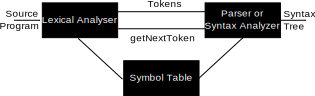
\includegraphics[width=.9\linewidth]{lexical_parser_relation}
		\end{center}
	\vfill
	\item There is three types of parsers for grammars: universal, top-down, bottom-up.
	\item But universal methods, such as the Cocke-Younger-Kasami algorithm and Earley's algorithm, are too inefficient.
	\item The most efficient top-down and bottom-up methods work only for subclasses of grammars: $LL$ and $LR$ grammars.
	\item But $LL$ and $LR$ grammars are expressive enough to describe most of the syntactic constructs in modern programming languages.
	\item $LL$ grammars are commonly used when writing a parser by hands
	\item $LR$ grammars are more complex and used in parser generators.
	\end{itemize}
\end{frame}

\subsection{Error recovery}

\sidecite{Dain.1991}
\begin{frame}{Handling of Syntax Errors}
	\begin{itemize}
	\item A compiler is expected to assist the programmer in locating and tracking down errors that inevitably creep into programs.
	\item Most programming language specifications do not describe how a compiler should respond to errors; error handling is left to the compiler designer.
	\vfill
	\item \alert{Why handling errors during the parsing?} \begin{itemize}
		\item $LL$ and $LR$ methods permits to detect errors efficiently and as soon as possible.
		\item Many errors appear syntactic, whatever they cause, and are exposed when parsing cannot continue.
		\end{itemize}
	\vfill
	\item \alert{The error handler must:} \begin{itemize}
		\item Report the presence of errors clearly and accurately.
		\item Recover from each error quickly to detect subsequent errors.
		\item Add minimal overhead to the processing of correct programs.
		\end{itemize}
	\end{itemize}
\end{frame}

\begin{frame}{Types of Programming Errors}
	\begin{description}
	\item[Lexical errors] they include misspellings of identifiers, keywords, or operators; and missing quotes around text intended as a string.
	\vfill
	\item[Syntactic errors] they include misplaced semicolons or extra or missing braces. Another example is a \kw{case} outside an enclosing \kw{switch} block.
	\vfill
	\item[Semantic errors] they include type mismatches between operators and operands.
	\vfill
	\item[Logical errors] they can be anything from incorrect reasoning on the part of the programmer to the use in a program. For example, the use of the operator \code{"="} in place of the operator \code{"=="}; or unreachable code.
	\end{description}
\end{frame}

\begin{frame}{Strategies for Error Recovery}
	\begin{small}
	\alertbox{Once an error is detected, how should the parser recover?}
	\vfill
	\begin{itemize}
	\item Although no strategy has proven itself universally acceptable.
	\vfill
	\item The simplest approach is for a parser to quit with an informative error message when it detects the first error; additional errors are uncovered.
	\vfill
	\item If errors pile up, it is better for the compiler to give up after exceeding some error limit than to produce an annoying avalanche of ``spurious'' errors.
	\vfill
	\item The rest of this section is devoted to the two major error-recovery strategies: \emph{panic mode}, and \emph{phrase-level recovery}.
	\end{itemize}
	\end{small}
\end{frame}

\begin{frame}{Panic Mode}
	\begin{itemize}
	\item The parser discards input symbols one at a time until one of a designated set of synchronizing tokens is found.
	\vfill
	\item The synchronizing tokens are usually delimiters, such as semicolons or closing braces, whose role in the source program is clear and unambiguous.
	\vfill
	\item This approach is simple to implement and it guarantees not to go into an infinite loop.
	\end{itemize}
\end{frame}

\begin{frame}{Phase-Level Recovery}
	\begin{itemize}
	\item On discovering an error, the parser may perform local correction on the remaining input:
		\begin{itemize}
		\item It may replace the prefix of the remaining input by some string that it allows the parser to continue; eg. replacing a coma by a semicolon, remove extraneous semicolon; or insert a missed semicolon
		\end{itemize}
	\vfill
	\item The choice of the correction is left to the compiler designer.
	\vfill
	\item The major drawback of the phrase-level recovery is the difficulty it has in coping with situations in which the actual error has occurred before the point of detection.
	\end{itemize}
\end{frame}

\begin{frame}{Error Productions}
	\begin{itemize}
	\item To anticipate the error detection, we can augment the grammar for the language at hand with productions that generate the erroneous constructs.
	\vfill
	\item A parser constructed from an augmented grammar detects the anticipated errors when an error production is used during parsing.
	\vfill
	\item The parser can then generate appropriate error diagnostics about the erroneous constructs that has been  recognized in the input.
	\end{itemize}
\end{frame}

\begin{frame}{Global Corrections}
	\begin{itemize}
	\item It would be helpful that a compiler makes few changes as possible in processing an incorrect input string.
	\vfill
	\item Given an incorrect input string \code{x} and grammar $G$, some algorithms find a parse tree for a related string \code{y}, such that the number of insertions, deletions, and changes of tokens required to transform \code{x} to \code{y} is as small as possible.
	\vfill
	\item \emph{Unfortunately, these methods are too costly in time and space.}
	\vfill
	\item Global corrections has been used to evaluate error-recovery algorithms and to find optimal replacement strings for phrase-level recovery.
	\end{itemize}
\end{frame}

\section{Context-free grammar}

\tableofcontentslide[sections={1-4},sectionstyle={show/shaded},subsectionstyle={show/show/hide},subsubsectionstyle={hide/hide/hide/hide}]

\subsection{Definition and notation}

\sidecite{Chomsky.1956, Backus.1959, Naur.1963, Ingerman.1967, Hopcroft.2006}
\begin{frame}[allowframebreaks]{What is a Context-Free Grammar?}
	\alertbox*{Grammars are systematically used to describe the syntax of programming language constructs.}
	\begin{itemize}
	\item A context-free grammar consists of \emph{terminals}, \emph{nonterminals}, a \emph{start symbol}, and \emph{productions}.
	\end{itemize}
	\begin{definition}[Terminal --- Token Name]
		The basic symbols from which strings are formed. \\
		It could be assimilated to a token, replied by the lexical analyzer (see Chapter~\ref{chap:lexical_analysis}).
	\end{definition}
	\begin{definition}[Nonterminals]
		Syntactic variables that denote sets of strings. \\
		The sets of strings denoted by nonterminals help to define the language generated by the grammar. Nonterminals impose a hierarchical structure on the language that is key to syntax analysis and translation.
	\end{definition}
	\begin{definition}[Production]
		The productions of a grammar specify the manner in which the terminals and nonterminals can be combined to form strings. Each production consists of: \begin{enumerate}
		\item A nonterminal called the \emph{head} or left side of the production; this production defines some of the strings denoted by the head.
		\item The symbol "$\rightarrow$" (or "\code{\string:\string:\string=}").
		\item A \emph{body}, or right side, consisting of zero or more terminals and nonterminals. The components of the body describe one way in which strings of the nonterminal at the head can be constructed.
		\end{enumerate}
	\end{definition}
	\begin{definition}[Start Symbol]
		In a grammar, one nonterminal is distinguished as the start symbol, and the set of strings it denotes is the language generated by the grammar. Conventionally, the productions for the start symbol are listed first.
	\end{definition}
\end{frame}

\begin{frame}{General Principles}
	\begin{enumerate}
	\item A grammar derives strings by beginning with the start symbol.
	\item It is repeatedly replacing a nonterminal by the body of a production for that nonterminal.
	\item The terminal strings, that can be derived, form the language defined by the grammar.
	\end{enumerate}
	\vfill
	\alertbox{Parsing is the problem of taking a string of terminals and figuring out how to derive it from the start symbol of the grammar. \\
		If the string cannot be derived, the parser reports a syntax error.}
\end{frame}

\begin{frame}[allowframebreaks]{Conventions on Notation}
	\begin{description}
	\item[These symbols are terminals]\begin{itemize}
		\item Lowercase letters early in the alphabet such as a, b, c, \dots
		\item Operator symbols, such as +, *, \dots
		\item Punctuation symbols, such as parentheses, commas, \dots
		\item The digits 0, \dots, 9.
		\item Boldface strings, such as \tok{id} or \tok{number}.
		\item Underlined strings, such as \underline{id} or \underline{number}.
		\end{itemize}
	\item[These symbols are nonterminals]\begin{itemize}
		\item Uppercase letters, such as A, B, C, \dots
		\item The letter \textit{S} which, when it appears, is usually the start symbol.
		\item Lowercase, italic names such as \textit{expression}, \textit{factor}, \dots
		\end{itemize}
	%
	\framebreak
	%
	\item[Productions] A set of productions $A \bnfbody a_1, A \bnfbody a_2, \dots, A \bnfbody a_k$ with a common head $A$ (call them $A$-productions), may be written $A \bnfbody a_1 \bnfor a_2 \bnfor \dots \bnfor a_k$ the alternatives of $A$.
	\item[Start Symbol] Unless stated otherwise, the head of the first production is the start symbol.
	\item[Others Notations]\begin{itemize}
		\item Uppercase letters late in the alphabet, such as X, Y, Z, represent grammar symbols that is, either nonterminals or terminals.
		\item Lowercase letters late in the alphabet, chiefly u, v, \dots, z, represent (possibly empty) strings of terminals.
		\item Lowercase Greek letters $\alpha$, $\beta$, \dots, represent (possibly empty) strings of grammar symbols.
		\end{itemize}
	\end{description}
\end{frame}

\begin{frame}[fragile]{Example of a Contect-Free Grammar}
	\begin{itemize}
	\item The arithmetic expressions are defined by the following grammar.
	\vfill
	\item The terminals are: \begin{description}
		\item[Operators] \code{+}, \code{-}, \code{*}, \code{/}, \code{(}, \code{)};
		\item[Numbers] \tok{number} stands for any number;
		\item[Identifier] \tok{id} stands for any variable's name.
		\end{description}
	\end{itemize}
	\vfill
	\begin{small}
	\begin{bnf}
	\p{ expression ::= expression \tok+ term}
	\p{            ::= expression \tok- term}
	\p{ term       ::= term \tok* factor}
	\p{            ::= term \tok/ factor}
	\p{            ::= factor}
	\p{ factor     ::= \tok( expression \tok)}
	\p{            ::= \tok{number}}
	\p{            ::= \tok{id}}
	\end{bnf}
	\end{small}
\end{frame}

\subsection{Derivations and Parse Tree}

\tableofcontentslide[sections={1-3},sectionstyle={show/shaded},subsectionstyle={show/shaded/hide},subsubsectionstyle={show/show/hide/hide}]

\subsubsection{Derivations}

\begin{frame}{Derivations}
	\begin{itemize}
	\item From the start symbol, each rewriting step replaces a nonterminal by the body of one of its productions.
	\vfill
	\item Let the example:
		\begin{center}\bnfstyle
			E \bnfbody E \tok+ E \bnfor E \tok* E \bnfor \tok- E \bnfor \tok( E \tok) \bnfor \tok{id}
		\end{center}
	\item The replacement of \textit{E} by \textit{\tok- E} will be described by writing:
		\begin{center}\bnfstyle
			E \deriv \tok- E
		\end{center}
	\item \emph{The symbol \deriv means ``derives in one step''.}
	\begin{example}
		\begin{itemize}
		\item Let a nonterminal \bnftext{A} in the middle of symbols: \bnftext{$\alpha$ A $\beta$}
		\item Let the production: \bnftext{A \bnfbody $\gamma$}
		\item Then: \bnftext{$\alpha$ A $\beta$ \deriv $\alpha$ $\gamma$ $\beta$}
		\end{itemize}
	\end{example}
	\end{itemize}
\end{frame}

\begin{frame}{Sequence of Derivations}
	\begin{definition}
		\begin{itemize}
		\item The sequence of derivations \bnftext{$a_1$ \deriv $a_2$ \deriv \dots \deriv $a_n$} rewrites $a_1$ to $a_n$.
		\item It may also be written: \bnftext{$a_1$ \seqderiv $a_n$}.
		\end{itemize}
	\end{definition}
	\begin{block}{Properties}
		\begin{enumerate}
		\item $\alpha\seqderiv\alpha$, for any string $\alpha$, and
		\item If $\alpha\seqderiv\beta$, and $\beta\deriv\gamma$, then $\alpha\seqderiv\gamma$.
		\end{enumerate}
	\end{block}
\end{frame}

\begin{frame}{Derivation as a Sentence of a Grammar}
	\begin{itemize}
	\item If \bnftext{S \seqderiv a}, where \bnftext{S} is the start symbol of a grammar $G$, we say that \bnftext{a} is a \emph{sentential form of $G$}.
	\vfill
	\item A sentence of $G$ is a sentential form, which is nonterminal.
	\vfill
	\item The language generated by $G$ is its set of sentences.
	\vfill
	\item A string of terminals \bnftext{w} is in $L(G)$ iff \bnftext{S \seqderiv w}. Thus $L(G)$ is said to be a context-free language.
	\end{itemize}
\end{frame}

\begin{frame}{Leftmost and Rightmost Derivations}
	\begin{itemize}
	\item At each step in a derivation, there are two choices to be made:
		\begin{enumerate}
		\item To choose which nonterminal to replace, and
		\item To pick a production with that nonterminal as head.
		\end{enumerate}
	\vfill
	\item To understand how parser work, we shall consider derivations in which the nonterminal to be replaced at each step is chosen as follows: \begin{description}
		\item[Leftmost derivation] the leftmost nonterminal in each sentential form is always chosen. If \bnftext{$\alpha$\deriv$\beta$} is a step in which the leftmost nonterminal in $\alpha$ is replaced, we write \bnftext{$\alpha$\derivlm$\beta$}.
		\item[Rightmost derivation] the rightmost nonterminal is always chosen, we write \bnftext{$\alpha$\derivrm$\beta$}.
		\end{description}
	\end{itemize}
\end{frame}

\begin{frame}[t]{Example of Leftmost Derivations}
	\begin{itemize}
	\item Let the grammar: \\
		\begin{small}
		\begin{bnf}
		\p{E ::= E \tok+ E}
		\p{  ::= E \tok* E}
		\p{  ::= \tok- E}
		\p{  ::= \tok( E \tok)}
		\p{  ::= \tok{id}}
		\end{bnf}
		\end{small}
	\item Let the input string: \texttt{2 + 4 * 6}
	\item Corresponding list of tokens: \tok{id}\tok+\tok{id}\tok*\tok{id}
	\item The leftmost derivations are:
	\end{itemize}
	\putat(160,-131){\mdseries\normalsize\normalcolor
		\begin{tabular}[t]{@{}p{1em}p{1em}l}
		\bnftext{E} & \derivlm & \bnftext{E \tok+ E} \\
		\only<2->{& \derivlm & \bnftext{\tok{id} \tok+ E} \\}
		\only<3->{& \derivlm & \bnftext{\tok{id} \tok+ E \tok* E} \\}
		\only<4->{& \derivlm & \bnftext{\tok{id} \tok+ \tok{id} \tok* E} \\}
		\only<5>{& \derivlm & \bnftext{\tok{id} \tok+ \tok{id} \tok* \tok{id}} \\}
		\end{tabular}
	}
\end{frame}

\begin{frame}[t]{Example of Rightmost Derivations}
	\begin{itemize}
	\item Let the grammar: \\
		\begin{small}
		\begin{bnf}
		\p{E ::= E \tok+ E}
		\p{  ::= E \tok* E}
		\p{  ::= \tok- E}
		\p{  ::= \tok( E \tok)}
		\p{  ::= \tok{id}}
		\end{bnf}
		\end{small}
	\item Let the input string: \texttt{2 + 4 * 6}
	\item Corresponding list of tokens: \tok{id}\tok+\tok{id}\tok*\tok{id}
	\item The leftmost derivations are:
	\end{itemize}
	\putat(160,-131){\mdseries\normalsize\normalcolor
		\begin{tabular}[t]{@{}p{1em}p{1em}l}
		\bnftext{E} & \derivrm & E \bnftext{\tok+ E} \\
		\only<2->{& \derivrm & \bnftext{E \tok+ E \tok* E} \\}
		\only<3->{& \derivrm & \bnftext{E \tok+ E \tok* \tok{id}} \\}
		\only<4->{& \derivrm & \bnftext{E \tok+ \tok{id} \tok* \tok{id}} \\}
		\only<5->{& \derivrm & \bnftext{\tok{id} \tok+ \tok{id} \tok* \tok{id}} \\}
		\end{tabular}
	}
\end{frame}

\subsubsection{Parse Tree}

\tableofcontentslide[sections={1-3},sectionstyle={show/shaded},subsectionstyle={show/shaded/hide},subsubsectionstyle={show/shaded/hide/hide}]

\begin{frame}{What is a Parse Tree?}
	\begin{small}
	\begin{definition}[Parse Tree]
	A parse tree shows how the start symbol of a grammar derives a string. It is a pictorial representation of the productions on an input string of tokens.
	\end{definition}
	\begin{block}{\small Building a Parse Tree}
		\begin{itemize}
		\item The root is labeled by the start symbol.
		\item Each leaf is labeled by a terminal or by $\epsilon$.
		\item Each interior node is labeled by a nonterminal.
		\item If $A$ is the nonterminal of some interior node and $X_1, X_2, \dots, X_n$ are the labels of the children of that node from left to right, then there must be a production $A \bnfbody X_1 X_2 \dots X_n$.
		\end{itemize}
	\end{block}
	\alertbox{Parsing is the process of building a parse tree.}
	\end{small}
\end{frame}

\begin{frame}{Example of a Parse Tree}
	\begin{columns}
		\begin{column}[t]{.5\linewidth}
			Let the string to parse:
				\begin{center}\texttt{9 - 5 + 2}\end{center}
			Let the grammar:\\[1em]
			\begin{scriptsize}
			\begin{bnf}
			\p{ expression ::= expression \tok+ term}
			\p{            ::= expression \tok- term}
			\p{ term       ::= term \tok* factor}
			\p{            ::= term \tok/ factor}
			\p{            ::= factor}
			\p{ factor     ::= \tok( expression \tok)}
			\p{            ::= \tok{number}}
			\p{            ::= \tok{id}}
			\end{bnf}
			\end{scriptsize}
		\end{column}
		\begin{column}[t]{.5\linewidth}
			The parse tree is:\\[1em]
			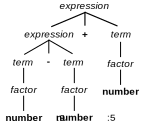
\includegraphics[width=.9\linewidth]{parse_tree_expr}
		\end{column}			
	\end{columns}
\end{frame}

\subsubsection{Building a Parse Tree with Derivations}

\tableofcontentslide[sections={1-3},sectionstyle={show/shaded},subsectionstyle={show/shaded/hide},subsubsectionstyle={show/shaded/hide/hide}]

\begin{frame}[b]{Algorithm to Build a Parse Tree with Derivations}
	\begin{scriptsize}
	\begin{myalgorithm}
	\SetKwFunction{node}{node}
	\SetKwFunction{nodelabel}{label}
	\SetKwFunction{nodechild}{addChild}
	\Input{A sequence of tokens $T$. A grammar $G$ with the start symbol $s_0$.}
	\Output{A parse tree that corresponds to $T$ and $G$.}
	\Begin{
		$r$ \affect \node($s_0$, $T$) ;	$L$ \affect $[r]$ ; $input[r]$ \affect $T$ \;
		\While(\tcc*[f]{Leftmost derivation}){$L = [n].L'$}{
			$L$ \affect $L'$ \;
			\If{$\exists (\nodelabel(n) \bnfbody b) \in G | input[n]$ matches $b$}{
				\ForEach{$\alpha s \beta = b$}{
					$m$ \affect $\omega \in T | (input[\alpha]\;\omega\;input[\beta]) = input[n]$ \;
					$c$ \affect \node($s$) \;
					\nodechild($n$,$c$) \;
					\If{$s$ is nonterminal}{
						$L$ \affect $L.[c]$ \;
						$input[c]$ \affect $m$ \;
					}
				}
			}
		}
		\Return $r$ \;
	}
	\end{myalgorithm}
	\end{scriptsize}
\end{frame}

\begin{frame}[t]{Example of Parse Tree Building}
	\begin{columns}
		\begin{column}[t]{.7\linewidth}
			Let the grammar: \\
			\begin{small}
			\begin{bnf}
			\p{E ::= E \tok+ E}
			\p{  ::= E \tok* E}
			\p{  ::= \tok- E}
			\p{  ::= \tok( E \tok)}
			\p{  ::= \tok{id}}
			\end{bnf}
			\end{small} \\[1em]
			Tokens: {\small \tok{id}\tok+\tok{id}\tok*\tok{id}} \\[1em]
			\begin{small}
			\only<1>{	$L = [E]$}
			\only<2>{	$L = [n].L' = [E]$ \\
					$input =$ \tok{id}\tok+\tok{id}\tok*\tok{id} \\
					$b =$ \bnftext{$E_0$ \tok+ $E_1$} \\
					$input_{E_0} =$ \tok{id} \\
					$input_{E_1} =$ \tok{id}\tok*\tok{id} \\
					$L = [E_0, E_1]$
			}
			\only<3,5>{	$L = [n].L' = [E, E]$ \\
					$input =$ \tok{id} \\
					$b =$ \tok{id} \\
					$L = [E]$
			}
			\only<4>{	$L = [n].L' = [E]$ \\
					$input =$ \tok{id}\tok*\tok{id} \\
					$b =$ \bnftext{$E_0$ \tok* $E_1$} \\
					$input_{E_0} =$ \tok{id} \\
					$input_{E_1} =$ \tok{id} \\
					$L = [E_0, E_1]$
			}
			\only<6>{	$L = [n].L' = [E]$ \\
					$input =$ \tok{id} \\
					$b =$ \tok{id} \\
					$L = []$
			}
			\end{small}
		\end{column}
		\begin{column}[t]{.3\linewidth}
			Parse tree is: \\[1em]
			\includeanimatedfigure[width=\linewidth]{parse_tree_example}
		\end{column}
	\end{columns}
\end{frame}

\subsection{Ambiguity of a grammar}

\tableofcontentslide[sections={1-4},sectionstyle={show/shaded},subsectionstyle={show/shaded/hide},subsubsectionstyle={show/show/hide/hide}]

\sidecite{Cantor.1962, Floyd.1962}
\begin{frame}{What is an Ambiguous Grammar?}
	\begin{small}
	\alertbox*{A grammar that produces more than one parse tree for some sentence is said to be ambiguous.}
	\begin{itemize}
	\item An ambiguous grammar is one that produces more than one leftmost derivation or more than one rightmost derivation for the same sentence.
	\end{itemize}
	\begin{example}
		Leftmost derivations for the arithmetic expression \tok{id}\tok+\tok{id}\tok*\tok{id}.
	\end{example}
	\end{small}
	\begin{tiny}
	\begin{tabular*}{\linewidth}{@{}c@{}|@{}c@{}}
		{\itshape	\begin{tabular}{lcl}
				E & \deriv & E \tok+ E \\
				  & \deriv & \tok{id} \tok+ E \\
				  & \deriv & \tok{id} \tok+ E \tok* E \\
				  & \deriv & \tok{id} \tok+ \tok{id} \tok* E \\
				  & \deriv & \tok{id} \tok+ \tok{id} \tok* \tok{id}
				\end{tabular}
				\raisebox{-.5\height}{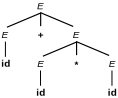
\includegraphics[width=.25\linewidth]{ambiguity_2}}
		}
	&
		{\itshape	\begin{tabular}{lcll}
				E & \deriv & E \tok* E \\
				  & \deriv & E \tok+ E \tok* E \\
				  & \deriv & \tok{id} \tok+ E \tok* E \\
				  & \deriv & \tok{id} \tok+ \tok{id} \tok* E \\
				  & \deriv & \tok{id} \tok+ \tok{id} \tok* \tok{id}
				\end{tabular}
				\raisebox{-.5\height}{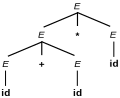
\includegraphics[width=.25\linewidth]{ambiguity_1}}
		}
	\end{tabular*}
	\end{tiny}
\end{frame}

\begin{frame}{Grammar Ambiguity is not Desirable}
	\begin{itemize}
	\item For parsers, it is desirable that the grammar be made unambiguous. Otherwise we cannot determine which parse tree to select for a sentence.
	\vfill
	\item Another way is to use carefully chosen ambiguous grammars, together with \emph{disambiguating rules} that discard undesirable parse trees, leaving only one tree for each sentence.
	\end{itemize}
\end{frame}

\subsection{Verifying the language supported by a grammar}

\tableofcontentslide[sections={1-4},sectionstyle={show/shaded},subsectionstyle={show/shaded/hide},subsubsectionstyle={show/show/hide/hide}]

\begin{frame}{Verifying the Language Supported by a Grammar}
	\begin{small}
	\begin{itemize}
	\item Even if compiler designers rarely do this task, it is useful to be able to verify if a language can be generated from a grammar.
	\vfill
	\item A proof that a grammar $G$ generates a language $L$ has two parts:
		\begin{enumerate}
		\item Show that every string generated by $G$ is in $L$.
		\item Show that every string in $L$ can be generated by $G$.
		\end{enumerate}
	\end{itemize}
	\begin{example}
		Considerer the following grammar:
		\begin{center}\bnfstyle S \bnfbody \tok( S \tok) S \bnfor \tok{e}\end{center}
		It may not be apparent, but this grammar generates all the strings of balanced parentheses, and only such strings.  That why, we need to proceed the two steps of the proof.
	\end{example}
	\end{small}
\end{frame}

\begin{frame}{Part 1: every string generated by $G$ is in $L$}
	\begin{description}
	\item[BASIS] The basis is $n=1$. The only string of terminals derivable from $S$ in one step is the empty string, which is balanced.
	\item[INDUCTION] Assume that all derivations of fewer than $n$ steps produce balanced sentences, and consider a leftmost derivation of exactly $n$ steps. Such a derivation must be of the form:
		\begin{center}\bnfstyle S \derivlm \tok( S \tok) S \derivlm \tok( x \tok) S \derivlm \tok( x \tok) y\end{center}
		The derivations of x and y from $S$ take fewer than $n$ steps, so by the inductive hypothesis $x$ and $y$ are balanced. Therefore, the string $\tok(x\tok)y$ must be balanced.
	\end{description}
\end{frame}

\begin{frame}{Part 2: every string in $L$ can be generated by $G$}
	\begin{description}
	\item[BASIS] If the string is length $0$, it must be $\epsilon$, which is balanced.
	\item[INDUCTION] Observe that every balanced string has even length. Assume that every balanced string of length less than $2n$ is derivable from $S$, and consider a balanced string $w$ of length $2n$, $n\ge1$. Surely $w$ begins with a left parenthesis. \\
		Let \bnftext{\tok(x\tok)} be the shortest nonempty prefix of $w$ having an equal number of left and right parentheses. \\
		Then $w$ can be written \bnftext{w = \tok(x\tok)y} where both $x$ and $y$ are balanced. Since $x$ and $y$ are of length less than $2n$, they are derivable from $S$ by the inductive hypothesis. Thus, we can find a derivation of the form:
			\begin{center}\bnfstyle S \deriv \tok( S \tok) S \seqderiv \tok( x \tok) S \seqderiv \tok( x \tok) y\end{center}
		proving that \bnftext{w = \tok(x\tok)y} is also derivable from $S$.
	\end{description}
\end{frame}

\subsection{Context-free grammar and regular expression}

\tableofcontentslide[sections={1-4},sectionstyle={show/shaded},subsectionstyle={show/shaded/hide},subsubsectionstyle={show/show/hide/hide}]

\begin{frame}{Context-Free Grammar \vs Regular Expression}
	\begin{itemize}
	\item \emph{Grammars are more powerful notation than regular expressions.}
	\item Every construct that can be described by a regular expression can be described by a grammar, but not vice-versa.
	\item For example the regular expression $(a|b)*abb$ and the following grammar describe the same language. \\
		\begin{bnf}
		\p{$A_0$ ::= \tok{a} $A_0$ \bnfor \tok{b} $A_0$ \bnfor \tok{a} $A_1$}
		\p{$A_1$ ::= \tok{b} $A_2$}
		\p{$A_2$ ::= \tok{b} $A_3$}
		\p{$A_3$ ::= $\epsilon$}
		\end{bnf}
	\item In the other hand, the language $L = { a^nb^n | n \ge 1 }$ is an example of a language that can be described by a grammar but not by a regular expression (except for Posix extension).
	\end{itemize}
\end{frame}

\begin{frame}{From Nondeterministic Finite Automaton to Grammar}
	\begin{itemize}
	\item It is possible to construct a grammar from a regular expression through the corresponding NFA.
	\vfill
	\item This mechanical transformation follows the steps below: \begin{enumerate}
		\item For each state $i$ of the NFA, create a nonterminal $A_i$.
		\item If state $i$ has a transition to state $j$ on input $a$, add the production \bnftext{$A_i$ \bnfbody a$A_j$}. If state $i$ goes to state $j$ on input $\epsilon$, add the production \bnftext{$A_i$ \bnfbody $A_j$}.
		\item If $i$ is an accepting state, add \bnftext{$A_i$ \bnfbody $\epsilon$}.
		\item If $i$ is the state state, make $A_i$ be the start symbol of the grammar.
		\end{enumerate}
	\end{itemize}
\end{frame}

\subsection{Guidelines for writing a grammar}

\subsubsection{General guidelines}

\tableofcontentslide[sectionstyle={show/shaded},subsectionstyle={show/shaded/hide},subsubsectionstyle={show/show/hide/hide}]

\begin{frame}[allowframebreaks]{General Guidelines for Writing a Grammar}
	\begin{itemize}
	\item Grammars are capable of describing most, but not all, of the syntax of programming languages.
		\begin{itemize}
		\item The requirement that identifiers be declared before they are used cannot be described in a grammar.
		\end{itemize}
	\item As seen previously, everything that can be described with a regular expression, can also be described y a grammar.
	\item Why use regular expressions to define the lexical syntax of a language?
		\begin{enumerate}
		\item Separating the syntactic structure of a language into lexical and non-lexical parts provides a better modularity.
		\item The lexical rules of a language are frequently quite simple, and to describe them we do not need a notation as complex as the grammars.
		\item Regular expressions generally provide a more concise and easier-to-understand notation for tokens than grammars.
		\item More efficient lexical analyzers can be constructed automatically from regular expressions than from arbitrary grammars.
		\end{enumerate}
	\item There a no firm guidelines as to what to put into the lexical rules, as opposed to the syntactic rules.
	\item Regular expressions are useful to describe constructs such as identifiers, numbers\dots
	\item Grammars are most useful for describing nested structures such as balanced parentheses, corresponding if-then-else\dots
	\end{itemize}
\end{frame}

\subsubsection{Eliminating the ambiguity}

\tableofcontentslide[sectionstyle={show/shaded},subsectionstyle={show/shaded/hide},subsubsectionstyle={show/shaded/hide/hide}]

\begin{frame}[t,allowframebreaks]{Example of Ambiguity Elimination: ``dangling else''}
	\begin{footnotesize}
	\alertbox{An ambiguous grammar can be rewritten to eliminate the ambiguity.}
	\begin{description}
	\item[Grammar]
			\begin{bnf}
			\p{statement ::= \tok{if} expression \tok{then} statement}
			\p{          ::= \tok{if} expression \tok{then} statement \tok{else} statement}
			\p{          ::= \tok{other}}
			\end{bnf}
	\item[Input] \tok{if} $E_1$ \tok{then} \tok{if} $E_2$ \tok{else} $S_1$ \tok{else} $S_2$
	\end{description}
	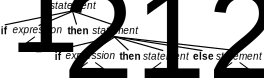
\includegraphics[width=.55\linewidth]{ambiguity_3}\hfill
	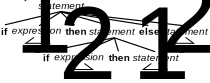
\includegraphics[width=.45\linewidth]{ambiguity_4}
	\begin{itemize}
	\item The first tree is preferred according to ``Match each \tok{else} with the closest unmatched \tok{then}.'' This rule is rarely built into productions.
	\end{itemize}
	\end{footnotesize}
	%
	\framebreak
	%
	\begin{footnotesize}
	The disambiguation of this ``if-then-else'' problem may be included into a new grammar.
	\begin{bnf}
	\p{statement ::= \tok{if} expression \tok{then} statement}
	\p{          ::= \tok{if} expression \tok{then} statement \tok{else} statement}
	\p{          ::= \tok{other}}
	\end{bnf}
	\begin{center}
\includegraphics[height=3em]{bottomarrow}\end{center}
	\begin{bnf}
	\p{statement ::= matched\_statement}%\tok{if} expression \tok{then} statement}
	\p{          ::= open\_statement}%
	\p{matched\_statement ::= \tok{if} expression \tok{then} matched\_statement \tok{else} matched\_statement}
	\p{                   ::= \tok{other}}
	\p{open\_statement ::= \tok{if} expression \tok{then} statement}
	\p{                ::= \tok{if} expression \tok{then} matched\_statement \tok{else} open\_statement}
	\end{bnf}
	\end{footnotesize}
\end{frame}

\subsubsection{Eliminating the left recursion}

\tableofcontentslide[sectionstyle={show/shaded},subsectionstyle={show/shaded/hide},subsubsectionstyle={show/shaded/hide/hide}]

\begin{frame}{Left Recursive Grammar}
	\begin{definition}[Left-Recursive Grammar]
		A grammar is left recursive if it has a nonterminal A such that there is a derivation $A \seqderivone A\alpha$ for some string $\alpha$.
	\end{definition}
	\alertbox{Top-down parsing methods cannot handler left-recursive grammars.}
	\begin{itemize}
	\vfill
	\item \emph{A transformation is needed to eliminate left recursion.}
	\vfill
	\item The algorithm to systematically eliminates left recursion from a grammar if the grammar has no cycle nor $\epsilon$-production: \begin{itemize}
		\item $\neg\left(A \seqderivone A\right)$ --- no cycle
		\item $\neg\left(A \bnfbody \epsilon\right)$ --- no $\epsilon$-production
		\end{itemize}
	\end{itemize}
\end{frame}

\begin{frame}{Eliminating Left Recursion}
	\begin{small}
	\begin{myalgorithm}
	\Input{Grammar $G$.}
	\Output{An equivalent grammar with no left recursion.}
	\Begin{
		\While{$\exists A | (A \bnfbody A\;\gamma) \in G$}{
			\ForEach{$p = (A \bnfbody b\;\delta) \in G | b \neq A$}{
				$G \affect G \setminus \{ p \}$ \;
				$G \affect G \cup \left\{ (R_A \bnfbody b\;\delta\;R_A) \right\}$ \;
			}
			$G = G \cup \left\{ (R_A \bnfbody \epsilon) \right\}$ \;
			\ForEach{$p = (A \bnfbody A\;\omega) \in G$}{
				$G \affect G \setminus \{ p \}$ \;
				$G \affect G \cup \left\{ (A \bnfbody \omega\;R_A) \right\}$ \;
			}
		}
	}
	\end{myalgorithm}
	\end{small}
\end{frame}

\begin{frame}{Example of Eliminating Left Recursion}
	\begin{tabularx}{\linewidth}{@{}XcX@{}}
		\begin{bnf}
		\p{E ::= E \tok+ E}
		\p{  ::= E \tok* E}
		\p{  ::= \tok- E}
		\p{  ::= \tok( E \tok)}
		\p{  ::= \tok{id}}
		\end{bnf}
	&
		
\includegraphics[width=3em]{rightarrow}
	&
		\begin{bnf}
		\p{E ::= \tok- E $R_E$}
		\p{  ::= \tok( E \tok) $R_E$}
		\p{  ::= \tok{id} $R_E$}
		\p{$R_E$ ::= \tok+ E $R_E$}
		\p{      ::= \tok* E $R_E$}
		\p{      ::= \ensuremath{\epsilon}}
		\end{bnf}
	\end{tabularx}
\end{frame}

\subsubsection{Left factoring}

\tableofcontentslide[sectionstyle={show/shaded},subsectionstyle={show/shaded/hide},subsubsectionstyle={show/shaded/hide/hide}]

\begin{frame}{Left Factoring}
	\begin{itemize}
	\item When the choice between two alternatives $A$-productions is not clear, we may be able to rewrite the productions to defer the decision until enough of the input has been seen that we can make the right choice.
	\end{itemize}
	\vfill
	\begin{small}\begin{center}
		\begin{bnf}[.9\linewidth]
		\p{statement ::= \tok{if} expression \tok{then} statement \tok{else} statement}
		\p{          ::= \tok{if} expression \tok{then} statement}
		\p{          ::= \tok{other}}
		\end{bnf}
	\end{center}\end{small}
	\vfill
	\alertbox*{Left factoring is a grammar transformation that is useful for producing a grammar suitable for predictive, or top-down, parsing.}
\end{frame}

\begin{frame}{Example of Left Factoring}
	\begin{small}\begin{center}
		\begin{bnf}[.9\linewidth]
		\p{statement ::= \tok{if} expression \tok{then} statement \tok{else} statement}
		\p{          ::= \tok{if} expression \tok{then} statement}
		\p{          ::= \tok{other}}
		\end{bnf} \\[1em]
		
\includegraphics[height=3em]{bottomarrow} \\[1em]
		\begin{bnf}[.95\linewidth]
		\p{statement ::= \tok{if} expression \tok{then} statement else\_statement}
		\p{          ::= \tok{other}}
		\p{else\_statement ::= \tok{else} statement}
		\p{                  ::= $\epsilon$}
		\end{bnf}
	\end{center}\end{small}
\end{frame}

\begin{frame}{Algorithm for Left Factoring}
	\begin{small}
	\begin{myalgorithm}
	\Input{Grammar $G$.}
	\Output{An equivalent left-factored grammar.}
	\BlankLine
	\Begin{
		\While{$\exists A  \in G | (A \bnfbody \alpha\;\gamma), (A \bnfbody \alpha\;\delta)$}{
			\ForEach{$p = (A \bnfbody \alpha\;\omega) \in G$}{
				$G \affect G \setminus \{ p \}$ \;
				\If{$\omega \neq \epsilon$}{
					$G \affect G \cup \left\{ (R_A \bnfbody \omega) \right\}$ \;
				}
			}
			$G \affect G \cup \left\{ (A \bnfbody \alpha\;R_A) \right\}$ \;
			$G \affect G \cup \left\{ (R_A \bnfbody \epsilon) \right\}$ \;
		}
	}
	\end{myalgorithm}
	\end{small}
\end{frame}

\section{Parsing with a grammar}

\tableofcontentslide[sectionstyle={show/shaded},subsectionstyle={show/show/hide},subsubsectionstyle={hide/hide/hide/hide}]

\subsection{Top-down parsing}

\tableofcontentslide[sectionstyle={show/shaded},subsectionstyle={show/shaded/hide},subsubsectionstyle={show/show/hide/hide}]

\subsubsection{Principles}

\begin{frame}{Top-Down Parsing}
	\begin{itemize}
	\item Top-down parsing can be viewed as the problem of constructing a parse tree for the input string, starting from the root and creating the nodes of the parse tree in preorder.
	\item Top-down parsing can be viewed as finding a leftmost derivation for an input string.
	\item The rest of this section uses the following grammar as illustration; and uses the input string \tok{id}\tok+\tok{id}\tok*\tok{id}.
	\end{itemize}
	\begin{small}
	\begin{center}
		\begin{bnf}[.4\linewidth]
		\p{E  ::= T E'}
		\p{E' ::= \tok+ T E'}
		\p{   ::= $\epsilon$}
		\p{T  ::= F T'}
		\p{T' ::= \tok* F T'}
		\p{   ::= $\epsilon$}
		\p{F  ::= \tok( E \tok)}
		\p{   ::= \tok{id}}
		\end{bnf}
	\end{center}
	\end{small}
\end{frame}

\begin{frame}{Types of Top-Down Parsing}
	\begin{itemize}
	\item Several top-down parsing methods exist, the two majors are:
		\begin{description}
		\vfill
		\item[Recursive-descent parsing] a general form, which may require backtracking to find the correct $A$-production to be applied.
		\vfill
		\item[Predictive parsing] a special case of recursive-descent parsing, where no backtracking is required. The $A$-production is chosen by looking ahead at the input a fixed number of symbols.
		\end{description}
	\vfill
	\item The class of grammars dedicated to the predictive parsers looking $k$ symbols ahead in the input is called $LL(k)$ class.
	\end{itemize}
\end{frame}

\subsubsection{Recursive-descent parsing}

\tableofcontentslide[sectionstyle={show/shaded},subsectionstyle={show/shaded/hide},subsubsectionstyle={show/shaded/hide/hide}]

\sidecite{Hoare.1962, Schorre.1964, McClure.1965}
\begin{frame}{Recursive-Descent Parsing}
	\begin{itemize}
	\item A recursive-descent parsing program consists of a set of procedures, one for each nonterminal.
	\vfill
	\item Execution begins with the procedure for the start symbol.
	\vfill
	\item The pseudo-code for each nonterminal is:
		\begin{scriptsize}
		\begin{myprocedure}{$A$}{}
		\SetKwFunction{call}{call}
		\Input{A production $A \bnfbody \alpha_1\dots\alpha_k$.}
		\Begin{
			\For{$i$ \affect $1$ \KwTo $k$}{
				\uIf{$\alpha_i$ is a nonterminal}{
					\call $\alpha_i$() \;
				}
				\uElseIf{$\alpha_i = $current input symbol $a$}{
					forward \affect forward + 1 \tcp*[f]{Move input pointer}\;
				}
				\Else{
					Report an error \;
				}
			}
		}
		\end{myprocedure}
		\end{scriptsize}
	\end{itemize}
\end{frame}

\begin{frame}{Problem of Infinite Loop}
	\begin{itemize}
	\item A left-recursive grammar can cause a recursive-descent parser to go into an infinite loop.
	\item That is, when we try to expand a nonterminal $A$, we may eventually find ourselves again trying to expand $A$ without having consumed input.
	\end{itemize}
	\vfill
	\begin{columns}
		\begin{column}{.5\linewidth}
			\begin{bnf}
			\p{E ::= E \tok+ E}
			\p{  ::= E \tok* E}
			\p{  ::= \tok- E}
			\p{  ::= \tok( E \tok)}
			\p{  ::= \tok{id}}
			\end{bnf}
		\end{column}
		\begin{column}{.5\linewidth}\bnfstyle
			\begin{tabular}{@{}ll@{}}
				E & \deriv E \tok+ E \\
				E & \deriv E \tok+ E \tok+ E \\
				E & \deriv E \tok+ E \tok+ E \tok+ E \\
				E & \deriv E \tok+ E \tok+ E \tok+ E \tok+ E \\
				& \deriv \dots
			\end{tabular}
		\end{column}
	\end{columns}	
\end{frame}

\subsubsection{FIRST and FOLLOW}

\tableofcontentslide[sectionstyle={show/shaded},subsectionstyle={show/shaded/hide},subsubsectionstyle={show/shaded/hide/hide}]

\begin{frame}{What are the Functions FIRST and FOLLOW?}
	\begin{itemize}
	\item The construction of both top-down and bottom-up parsers is aided by two functions associated with a grammar G:
		\begin{enumerate}
		\item FIRST
		\item FOLLOW
		\end{enumerate}
	\vfill
	\item These functions allow us to choose which production to apply, based on the next input symbol.
	\vfill
	\item During panic-mode error recovery the set of tokens replied by FOLLOW can be used as synchronizing tokens.
	\end{itemize}
\end{frame}

\begin{frame}{Definition of FIRST}
	\begin{itemize}
	\item Define FIRST($\alpha$), where $\alpha$ is any string of grammar symbols, to be the set of terminals that begin strings derived from $\alpha$.
	\item If $\alpha \seqderiv \epsilon$, then $\epsilon$ is also in FIRST($\alpha$).
	\end{itemize}
	\vfill
	\begin{example}\bnfstyle
		\begin{columns}
			\begin{column}[t]{.4\linewidth}
				$A \seqderiv c\;\gamma$ \\
				FIRST($A$) $ = \{ c \}$
			\end{column}
			\begin{column}[t]{.4\linewidth}
				\raisebox{-\height}{\includegraphicswtex[width=\linewidth]{example_FIRST}}
			\end{column}
		\end{columns}
	\end{example}
\end{frame}

\begin{frame}{Algorithm of FIRST}
	\begin{itemize}
	\item To compute FIRST($X$) for a grammar symbol $X$, apply the following rules until no more terminals or $\epsilon$ can be added to any FIRST set.
	\vfill
		\begin{enumerate}
		\item If $X$ is a terminal, then FIRST($X$) $= \{ X \}$.
		\item If $X$ is a nonterminal and $X \bnfbody Y_1\;Y_2 \dots Y_k$ is a production for some $k \ge 1$, then place $a$ in FIRST($X$) if for some $i$, $a$ is in FIRST($Y_i$), and $\epsilon$ is in all of FIRST($Y_1$), \dots, FIRST($Y_{k-1}$); that is, $Y_1\;Y_2 \dots Y_k \seqderiv \epsilon$. If $\epsilon$ is in FIRST($Y_j$) for all $j \in \{1, 2, \dots, k\}$, then add $\epsilon$ to FIRST($X$).
		\item If $X \bnfbody \epsilon$ is a production, then add $\epsilon$ to FIRST($X$).
		\end{enumerate}
	\vfill
	\item Add to FIRST($X_1\;X_2 \dots X_n$) all non-$\epsilon$ symbols of FIRST($X_i$) for $i \in \{1 \dots n\}$.
	\end{itemize}
\end{frame}

\begin{frame}{Definition of FOLLOW}
	\begin{scriptsize}
	\begin{itemize}
	\item Define FOLLOW($A$), where $A$ is a nonterminal, to be the set of terminals a that can appear immediately to the right of $A$ in some sentential form.
	\item The set of terminals a such that there exists a derivation of the form $S \seqderiv \alpha\;A\;a\;\beta$, for some $\alpha$ and $\beta$.
	\item Note that there may have been symbols between $A$ and $a$, at some time during the derivation, but if so, they derive $\epsilon$ and disappeared.
	\item If $A$ can be the rightmost symbol, then \tok{eof} (or usually \tok{\$}) is in FOLLOW($A$).
	\end{itemize}
	\end{scriptsize}
	\vfill
	\begin{small}
	\begin{example}\bnfstyle
		\begin{columns}
			\begin{column}[t]{.4\linewidth}
				$A \seqderiv c\;\gamma$ \\
				$a \in $FOLLOW($A$)
			\end{column}
			\begin{column}[t]{.4\linewidth}
				\raisebox{-\height}{\includegraphicswtex[width=\linewidth]{example_FIRST}}
			\end{column}
		\end{columns}
	\end{example}
	\end{small}
\end{frame}

\begin{frame}{Algorithm of FOLLOW}
	\begin{itemize}
	\item To compute FOLLOW($A$) for a nonterminal $A$, apply the following rules until nothing can be added to any FOLLOW set.
		\begin{enumerate}
		\vfill
		\item Place \tok{eof} in FOLLOW($S$), where $S$ is the start symbol, and \tok{eof} is the input right endmarker.
		\vfill
		\item If there is a production \bnftext{A \bnfbody $\alpha\;B\;\beta$}, then everything in FIRST($b$), except $\epsilon$ is in FOLLOW($B$).
		\vfill
		\item If there is a production \bnftext{A \bnfbody $\alpha\;B$}, or a production \bnftext{A \bnfbody $\alpha\;B\;\beta$}, where FIRST($\beta$) contains $\epsilon$, then everything in FOLLOW($A$) is in FOLLOW($B$).
		\end{enumerate}
	\end{itemize}
\end{frame}

\subsubsection{$LL(1)$ grammars}

\tableofcontentslide[sectionstyle={show/shaded},subsectionstyle={show/shaded/hide},subsubsectionstyle={show/shaded/hide/hide}]

\sidecite{Lewis.1968, Birman.1973}
\begin{frame}{$LL(1)$ Grammar}
	\begin{itemize}
	\item Predictive parsers, that is, recursive-descent parsers needing no backtracking, can be constructed for a class of grammars called $LL(1)$.
	\vfill
		\begin{itemize}
		\item \Emph{L}eft-to-right input scanning,
		\item \Emph{L}eftmost derivation,
		\item \Emph{1} input symbol is used for lookahead to make parsing action decisions.
		\end{itemize}
	\vfill
	\item The class of $LL(1)$ grammars is rich enough to cover most programming constructs, although care is needed in writing a suitable grammar for the source language \eg no left-recursive nor ambiguous grammar can be $LL(1)$.
	\end{itemize}
\end{frame}

\begin{frame}{Definition of a $LL(1)$ Grammar}
	\begin{itemize}
	\item A grammar $G$ is $LL(1)$ iff whenever \bnftext{A \bnfbody $\alpha$ \bnfor $\beta$} are two distinct productions of $G$, the following conditions hold:
		\begin{enumerate}
		\vfill
		\item For nonterminal $a$ do both $\alpha$ and $\beta$ derive strings beginning with $a$.
		\vfill
		\item At most one of $\alpha$ and $\beta$ can derive the empty string.
		\vfill
		\item If $\beta\seqderiv\epsilon$, then $\alpha$ does not derive any string beginning with a terminal in FOLLOW($A$). Likewise, if $\alpha\seqderiv\epsilon$, then $\beta$ does not derive any string beginning with a terminal in FOLLOW($A$).
		\end{enumerate}
	\end{itemize}
	\vfill
	\begin{small}
	\begin{bnf}
	\p{statement\_list ::= statement statement\_list}
	\p{                ::= $\epsilon$}
	\p{statement ::= \tok{if} \tok( expression \tok) statement \tok{else} statement}
	\p{          ::= \tok{while} \tok( expression \tok) statement}
	\p{          ::= \tok\{ statement\_list \tok\}}
	\end{bnf}
	\end{small}
\end{frame}

\begin{frame}{Parsing a $LL(1)$ Grammar}
	\alertbox{To parse an input string, a table should be build. It permits to determine the production to use from a given production and the input symbol.}
	\vfill
	\begin{itemize}
	\item The following algorithm permits to collects informations from FIRST and FOLLOW sets into a predictive parsing table $M[A,a]$, where $A$ is a nonterminal, and $a$ is a terminal or \tok{eof}.
	\end{itemize}
\end{frame}

\begin{frame}[allowframebreaks]{Algorithm for Building the Predicitve-Parsing Table}
	\vfill
	\begin{itemize}
	\item The algorithm is based on the idea:
		\begin{enumerate}
		\item The production \bnftext{A \bnfbody $\alpha$} is chosen if the next input symbol $a \in $FIRST($\alpha$).
		\item When $\alpha\seqderiv\epsilon$, we should again choose \bnftext{A \bnfbody $\alpha$}, of the current input symbol is in FOLLOW($A$), or if the \tok{eof} on the input has been reached and \tok{eof} is in FOLLOW($A$).
		\end{enumerate}
	\vfill
	\item If a cell of the predictive parsing table contains more than one information, then the grammar associated to the table is ambiguous.
	\end{itemize}
	\vfill
	%	
	\framebreak
	%
	\begin{description}
	\item[INPUT] Grammar $G$.
	\item[OUTPUT] Parsing table $M$.
	\item[METHOD] For each production \bnftext{A \bnfbody $\alpha$} of the grammar, do the following:
		\begin{itemize}
		\item For each terminal $a$ in FIRST($\alpha$), add \bnftext{A \bnfbody $\alpha$} to $M[A,a]$.
		\item If $\epsilon$ is in FIRST($\alpha$), then for each terminal $b$ in FOLLOW($A$), add \bnftext{A \bnfbody $\alpha$} to $M[A,b]$.
		\item If $\epsilon$ is in FIRST($\alpha$) and \tok{eof} is in FOLLOW($A$), add \bnftext{A \bnfbody $\alpha$} to $M[A,\tok{eof}]$ as well.
		\end{itemize}
		\vspace{1em}
		If, after performing the above, there is no production in $M[A,a]$, then set $M[A,a]$ to error (generally replaced by an empty string in the table).
	\end{description}
\end{frame}

\begin{frame}[t]{Example of Table Building}
	\begin{scriptsize}
	\begin{bnf}[.33\linewidth]
	\p[1]{E  ::= T E'}
	\p[2]{E' ::= \tok+ T E'}
	\p[3]{   ::= $\epsilon$}
	\p[4]{T  ::= F T'}
	\p[5]{T' ::= \tok* F T'}
	\p[6]{   ::= $\epsilon$}
	\p[7]{F  ::= \tok( E \tok)}
	\p[8]{   ::= \tok{id}}
	\end{bnf}
	\end{scriptsize} \\[1em]
	\begin{small}\bnfstyle
	\begin{tabularx}{\linewidth}{|c|X|X|X|X|X|X|}
		\hline
		\tabularheading&\chead{\tok{id}}&\chead{\tok+}&\chead{\tok*}&\chead{\tok(}&\chead{\tok)}&\chead{\tok{eof}} \\
		\hline
		E & \only<2->{\bnfmark{1}} & & & \only<2->{\bnfmark{1}} & & \\
		\hline
		E' & & \only<3->{\bnfmark{2}} & & & \only<4->{\bnfmark{3}} & \only<5->{\bnfmark{3}} \\
		\hline
		T & \only<6->{\bnfmark{4}} & & & \only<6->{\bnfmark{4}} & & \\
		\hline
		T' & & \only<8->{\bnfmark{6}} & \only<7->{\bnfmark{5}} & & \only<8->{\bnfmark{6}} & \only<8->{\bnfmark{6}} \\
		\hline
		F & \only<10->{\bnfmark{8}} & & & \only<9->{\bnfmark{7}} & & \\
		\hline
	\end{tabularx}
	\end{small}
	\begin{scriptsize}
	\putat(110,-10){\parbox[t]{.55\paperwidth}{\normalfont\normalcolor\small
		\only<1-2>{	\Emph{For production:} \bnfmark{1}~\bnftext{E \bnfbody T E'} \\
				FIRST($T E'$) = FIRST($T$) = FIRST($F$) = $\{ \tok(, \tok{id} \}$ \\
				\only<2>{Then put the production in $M[E,\tok(]$ and $M[E,\tok{id}]$; the rest of the line is \emph{error}}
		}
		\only<3>{	\Emph{For production:} \bnfmark{2}~\bnftext{E' \bnfbody \tok+ T E'} \\
				FIRST($\tok+ T E'$) = $\{ \tok+ \}$ \\
				Then put the production in $M[E',\tok+]$
		}
		\only<4,5>{	\Emph{For production:} \bnfmark{3}~\bnftext{E' \bnfbody $\epsilon$} \\
				FIRST($\epsilon$) = $\{ \epsilon \}$ \\
				FOLLOW($E'$) = $\{ \tok), \tok{eof} \}$ \\
				Put the production in $M[E',\tok)]$ (rule 2) \\
				\only<5>{Put the production in $M[E',\tok{eof}]$ (rule 3)}
		}
		\only<6>{	\Emph{For production:} \bnfmark{4}~\bnftext{T \bnfbody F T'} \\
				FIRST($F\;T'$) = FIRST($F$) = $\{ \tok(, \tok{id} \}$ \\
				Put the production in $M[T,\tok(]$ and $M[T,\tok{id}]$
		}
		\only<7>{	\Emph{For production:} \bnfmark{5}~\bnftext{T' \bnfbody \tok* F T'} \\
				FIRST($\tok*\;F\;T'$) = $\{ \tok* \}$ \\
				Put the production in $M[T',\tok*]$
		}
		\only<8>{	\Emph{For production:} \bnfmark{6}~\bnftext{T' \bnfbody $\epsilon$} \\
				FIRST($\epsilon$) = $\{ \epsilon \}$ \\
				FOLLOW($T'$) = $\{ \tok+, \tok), \tok{eof} \}$ \\
				Put the production in $M[T',\tok+]$ and $M[T,\tok)]$ (rule 2) \\
				Put the production in $M[T',\tok{eof}]$ (rule 3)
		}
		\only<9>{	\Emph{For production:} \bnfmark{7}~\bnftext{F \bnfbody \tok( E \tok)} \\
				FIRST($\tok(\;E\tok)$) = $\{ \tok( \}$ \\
				Put the production in $M[F,\tok(]$
		}
		\only<10>{	\Emph{For production:} \bnfmark{9}~\bnftext{F \bnfbody \tok{id}} \\
				FIRST(\tok{id}) = $\{ \tok{id} \}$ \\
				Put the production in $M[F,\tok{id}]$
		}
	}}
	\end{scriptsize}
\end{frame}

\subsubsection{Nonrecursive predictive parsing}

\tableofcontentslide[sectionstyle={show/shaded},subsectionstyle={show/shaded/hide},subsubsectionstyle={show/shaded/hide/hide}]

\begin{frame}{Nonrecursive Predictive Parsing}
	\begin{itemize}
	\item A nonrecursive predictive parser can be built by maintaining a stack explicitly, rather than implicitly via recursive calls.
	\item The parser mimics a leftmost derivation. If \code{w} is the input that has been matched so far, then the stack holds a sequence of grammar symbols a such that:
		\begin{center}
			$S \seqderiv w\;\alpha$
		\end{center}
	\item The table-driven parser has an \emph{input buffer}, a \emph{stack} containing a sequence of grammar symbols, a \emph{parsing table}, and an \emph{output stream}.
	\end{itemize}
	\begin{center}
		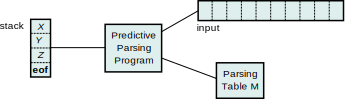
\includegraphics[width=.8\linewidth]{nonrecursive_predictive_parser}
	\end{center}
\end{frame}

\begin{frame}{Algorithm of the Nonrecursive Predictive Parsing}
	\begin{tiny}
	\begin{myalgorithm}
	\SetKwFunction{inputSymbol}{inputSymbol}
	\SetKwFunction{nextInputSymbol}{nextInputSymbol}
	\SetKwFunction{pop}{pop}
	\SetKwFunction{push}{push}
	\SetKwFunction{topOf}{topOf}
	\SetKwFunction{print}{print}
	\Input{A string \code{w}, a parsing table $M$ for grammar $G$, and a start symbol $s_0$.}
	\Output{If \code{w} is in $L(G)$, a lefmost derivation of \code{w}; otherwise, an error indication.}
	\Begin{
		$a$ \affect \inputSymbol()\;
		\push($S$, \tok{eof}) \;
		\push($S$, $s_0$) \;
		\While{$\topOf(S) \neq \tok{eof}$}{
			$X$ \affect \topOf($S$) \;
			\uIf{$X = a$}{
				\pop($S$); $a$ \affect \nextInputSymbol()\;
			}
			\uElseIf{$X$ is a terminal}{
				Report an error\;
			}
			\uElseIf{$M[X,a] = X \bnfbody Y_1 \dots Y_n$}{
				\print($X \bnfbody Y_1 \dots Y_n$)\;
				\pop($S$)\;
				\lFor{$i$ \affect $n$ \KwTo $1$}{\push($S, Y_i$)} \;
			}
			\Else{
				 Report an error\tcp*[f]{$M[X,a]$ is empty}\;
			}
		}
	}
	\end{myalgorithm}
	\end{tiny}
\end{frame}

\pgfdeclareimage[width=2em]{rightarrow_2em}{imgs/all/rightarrow}

\begin{frame}{Example of Nonrecursive Predictive Parsing}
	\only<1>{\putat(-30,-27){\pgfuseimage{rightarrow_2em}}}
	\only<2>{\putat(-30,-34){\pgfuseimage{rightarrow_2em}}}
	\only<3>{\putat(-30,-41){\pgfuseimage{rightarrow_2em}}}
	\only<4,8,12,16,18,22>{\putat(-30,-53){\pgfuseimage{rightarrow_2em}}}
	\only<5,9,13,19,23>{\putat(-30,-94){\pgfuseimage{rightarrow_2em}}}
	\only<6,10,14,20,24>{\putat(-30,-101){\pgfuseimage{rightarrow_2em}}}
	\only<7,11,15,21,25>{\putat(-30,-108){\pgfuseimage{rightarrow_2em}}}
	\only<17>{\putat(-30,-67){\pgfuseimage{rightarrow_2em}}}
	\begin{tiny}
	\begin{columns}
		\begin{column}{.5\linewidth}
		\begin{myalgorithm}
		\SetKwFunction{inputSymbol}{inputSymbol}
		\SetKwFunction{nextInputSymbol}{nextInputSymbol}
		\SetKwFunction{pop}{pop}
		\SetKwFunction{push}{push}
		\SetKwFunction{topOf}{topOf}
		\SetKwFunction{print}{print}
		\Begin{
			$a$ \affect \inputSymbol()\;
			\push($S$, \tok{eof}) \;
			\push($S$, $s_0$) \;
			\While{$\topOf(S) \neq \tok{eof}$}{
				$X$ \affect \topOf($S$) \;
				\uIf{$X = a$}{
					\pop($S$); $a$ \affect \nextInputSymbol()\;
				}
				\uElseIf{$X$ is a terminal}{
					Report an error\;
				}
				\uElseIf{$M[X,a] = X \bnfbody Y_1 \dots Y_n$}{
					\print($X \bnfbody Y_1 \dots Y_n$)\;
					\pop($S$)\;
					\lFor{$i$ \affect $n$ \KwTo $1$}{\push($S, Y_i$)} \;
				}
				\Else{
					 Report an error\;
				}
			}
		}
		\end{myalgorithm}
		\end{column}
		\begin{column}[t]{.5\linewidth}
			\raisebox{-.5\height}{\includeanimatedfigure[width=\linewidth]{nonrecursive_predictive_parsing_example}}
		\end{column}
	\end{columns}
	\vspace{-.5em}
	\begin{tabularx}{.6\linewidth}[t]{|c|X|X|X|X|X|X|}
		\hline
		\tabularheading&\chead{\tok{id}}&\chead{\tok+}&\chead{\tok*}&\chead{\tok(}&\chead{\tok)}&\chead{\tok{eof}} \\
		\hline
		E & \bnfmark{1} & & & \bnfmark{1} & & \\
		\hline
		E' & & \bnfmark{2} & & & \bnfmark{3} & \bnfmark{3} \\
		\hline
		T & \bnfmark{4} & & & \bnfmark{4} & & \\
		\hline
		T' & & \bnfmark{6} & \bnfmark{5} & & \bnfmark{6} & \bnfmark{6} \\
		\hline
		F & \bnfmark{8} & & & \bnfmark{7} & & \\
		\hline
	\end{tabularx}
	\hfill
	\raisebox{-\height}{\begin{bnf}[.33\linewidth]
	\p[1]{E  ::= T E'}
	\p[2]{E' ::= \tok+ T E'}
	\p[3]{   ::= $\epsilon$}
	\p[4]{T  ::= F T'}
	\p[5]{T' ::= \tok* F T'}
	\p[6]{   ::= $\epsilon$}
	\p[7]{F  ::= \tok( E \tok)}
	\p[8]{   ::= \tok{id}}
	\end{bnf}}
	\end{tiny}
\end{frame}

\subsubsection{Error recovery in predictive parsing}

\tableofcontentslide[sectionstyle={show/shaded},subsectionstyle={show/shaded/hide},subsubsectionstyle={show/shaded/hide/hide}]

\begin{frame}[allowframebreaks]{Panic Mode}
	\begin{itemize}
	\item \emph{Panic-mode error recovery is based on the idea of skipping over symbols on the input until a token in a selected set of synchronizing tokens appears.}
	\item Its effectiveness depends on the choice of synchronizing set.
	\item The sets should be chosen so that the parser recovers quickly from errors that are likely to occur in practice.
	\item Some heuristics are as follows:
		\begin{enumerate}
		\item As a starting point, place all symbols in FOLLOW($A$) into the synchronizing set for nonterminal $A$. If we skip tokens until an element of FOLLOW($A$) is seen and pop $A$ from the stack, it is likely that parsing can continue.
		\item It is not enough to use FOLLOW($A$) as the synchronizing set for $A$. We can add to the set of a lower-level construct the symbols that begin higher-level constructs. For example, we might add keywords that begin statements to the synchronizing sets for the nonterminals generating expressions.
		\item If we add symbols in FIRST($A$) to the synchronizing set for nonterminal $A$, then it may be possible to resume parsing according to $A$ if a symbol in FIRST($A$) appears in the input.
		\item If a nonterminal can generate the empty string, then the production deriving $\epsilon$ can be used as a default. Doing so may postpone some error detection, but cannot cause an error to be missed. This approach reduces the number of nonterminals that have to be considered during error recovery.
		\item If a terminal on top of the stack cannot be matched, a simple idea is to pop the terminal, issue a message saying that the terminal was inserted, and continue parsing. In effect, this approach takes the synchronizing set of a token to consist of all other tokens.
		\end{enumerate}
	\end{itemize}
\end{frame}

\subsection{Bottom-up parsing}

\tableofcontentslide[sectionstyle={show/shaded},subsectionstyle={show/shaded/hide},subsubsectionstyle={show/show/hide/hide}]

\sidecite{Knuth.1965, Korenjak.1969}
\begin{frame}{Bottom-Up Parsing}
	\begin{itemize}
	\item A bottom-up parsing corresponds to the construction of a parse tree for an input string beginning at the leaves (the bottom) and working up towards the root.
	\vfill
	\item This section introduces a general style bottom-up parsing known as \emph{shift-reduce parsing}, which is attached the class of the $LR$ grammars.
	\vfill
	\item \emph{$LR$ parsers are too difficult to be written by hand. We prefer to use automatic parser generators in place.}
	\end{itemize}
\end{frame}

\subsubsection{Reductions}

\tableofcontentslide[sectionstyle={show/shaded},subsectionstyle={show/shaded/hide},subsubsectionstyle={show/shaded/hide/hide}]

\begin{frame}{Principle of Reduction}
	\begin{itemize}
	\item The bottom-up parsing is the process of ``reducing'' a string w to the start symbol of the grammar.
	\vfill
	\item At each reduction step, a specific substring matching the body of a production is replaced by the nonterminal at the head of that production.
	\vfill
	\item The key decisions during bottom-up parsing are about when to reduce and about what production to apply, as the parse proceeds.
	\vfill
	\item By definition, a reduction is the reverse of a step in a derivation. \emph{The goal of the bottom-up parsing is therefore to construct a derivation in reverse.}
	\end{itemize}
\end{frame}

\begin{frame}[t]{Example of Reductions}
	\begin{small}
	\begin{itemize}
	\item Let the grammar:
		\raisebox{-.75\height}{
		\begin{scriptsize}
		\begin{bnf}[.33\linewidth]
		\p{E  ::= T E'}
		\p{E' ::= \tok+ T E'}
		\p{   ::= $\epsilon$}
		\p{T  ::= F T'}
		\p{T' ::= \tok* F T'}
		\p{   ::= $\epsilon$}
		\p{F  ::= \tok( E \tok)}
		\p{   ::= \tok{id}}
		\end{bnf}
		\end{scriptsize}}
	\item A possible sequence of reductions is: \\
		\bnftext{\only<1->{\tok{id}~\tok*~\tok{id}
				\reduce~F~\tok*~\tok{id}
				\reduce~F~\tok*~F
				\reduce~F~\tok*~F~$\epsilon$
				\reduce~F~\tok*~F~T'
				\reduce~F~T'} \\
			\only<2>{\reduce~T
				\reduce~T~$\epsilon$
				\reduce~T~E'
				\reduce~E}
		}
	\end{itemize}
	\end{small}
	\vfill
	\begin{center}
	\includeanimatedfigure[height=.25\paperheight]{reduction_example}
	\end{center}
\end{frame}

\begin{frame}{How to Find the Best Reductions?}
	\alertbox{What is the best sequence of reductions to build the parse tree?}
	\vspace{4em}
	\begin{itemize}
	\item One method is to use the \emph{shift-reduce parsing} method.
	\vspace{2em}
	\item The shift-reduce method is based on the \emph{handle pruning}.
	\end{itemize}
\end{frame}

\subsubsection{Handle pruning}

\tableofcontentslide[sectionstyle={show/shaded},subsectionstyle={show/shaded/hide},subsubsectionstyle={show/shaded/hide/hide}]

\begin{frame}{Definition of a Handle}
	\begin{itemize}
	\item Informally, a \emph{handle} is a substring that matches the body of a production, and whose reduction represents one step along the reverse of a rightmost derivation.
	\item If $S \seqderivrm \alpha\;A\;\omega \derivrm \alpha\;\beta\;\omega$, then production \bnftext{A \bnfbody $\beta$} in the position following $\alpha$ is a handle of $\alpha\beta\omega$.
		\begin{center}
		\includegraphicswtex[width=.4\linewidth]{handle_definition}
		\end{center}
	\item A handle of a right-sentential form $\gamma$ is a production \bnftext{A \bnfbody $\beta$} and a position of $\gamma$ where the string $\beta$ may be found, such that replacing $\beta$ at that position by $A$ produces the previous right-sentential form in a rightmost derivation of $\gamma$.
	\item \emph{Note that $\omega$ must contain only terminal symbols.}
	\end{itemize}
\end{frame}

\begin{frame}[t]{Algorithm of Handle Pruning}
	\begin{scriptsize}
	\begin{myalgorithm}
	\SetKwInOut{hypothesis}{Hypothesis}
	\Input{A string of terminals $\omega$. A grammar $G$.}
	\Output{A sequence of reductions of $\omega$, or an error if no sequence was found.}
	\hypothesis{$w = \gamma_n$, where $\gamma_n$ is the n\textup{th} right-sentential form of some, \Emph{yet unknown}, rightmost derivation: $S = \gamma_0 \derivrm \gamma_1 \derivrm \gamma_2 \seqderivrm \gamma_{n-1} \derivrm \gamma_n = \omega$}
	\Begin{
		$d \affect []$; $f \affect \omega$\;
		\While{$f \neq S$}{
			\uIf{$\exists h \in f | f = \alpha\;h\;\beta\;;\,\beta$ contains only terminals}{
				\uIf{$\exists p \in G | p = (A \bnfbody h)$}{
					$f \affect \alpha\;p\;\beta$\;
					$d \affect [(\alpha\;h\;\beta)].d$\;
				}
				\Else{
					\throw{\str{"Cannot find a production for reduction"}}\;
				}
			}
			\Else{
				\throw{\str{"Cannot find a handle"}}\;
			}
		}
		\Return $d$\;
	}
	\end{myalgorithm}
	\end{scriptsize}
\end{frame}

\subsubsection{Shift-reduce parsing}

\tableofcontentslide[sectionstyle={show/shaded},subsectionstyle={show/shaded/hide},subsubsectionstyle={show/shaded/hide/hide}]

\begin{frame}{Shift-Reduce Parsing}
	\begin{itemize}
	\item Shift-reduce parsing is a form of bottom-up parsing in which a \emph{stack holds grammar symbols} and an \emph{input buffer holds the rest of the string} to be parsed.
	\item The handle always appears at the top of the stack just before it is identified as the handle.
	\vfill
	\item The four operations available during shift-reduce parsing are:
		\begin{description}
		\item[Shift] Shift the next input symbol onto the top of the stack.
		\item[Reduce] The right end of the string to be reduced must be at the top of the stack. Locate the left end of the string within the stack and decide with what nonterminal to replace the string.
		\item[Accept] Announce successful completion of parsing.
		\item[Error] Discover a syntax error and call an error recovery routine.
		\end{description}
	\end{itemize}
\end{frame}

\begin{frame}{Example of Shift-Reduce Parsing}
	\begin{footnotesize}
	\raisebox{-\height}{\begin{bnf}[.33\linewidth]
	\p{E  ::= T E'}
	\p{E' ::= \tok+ T E'}
	\p{   ::= $\epsilon$}
	\p{T  ::= F T'}
	\p{T' ::= \tok* F T'}
	\p{   ::= $\epsilon$}
	\p{F  ::= \tok( E \tok)}
	\p{   ::= \tok{id}}
	\end{bnf}}
	\end{footnotesize}
	\hfill
	\raisebox{-.5\height}{\includeanimatedfigure[width=.65\linewidth]{shift_reduce_parsing_example}}
\end{frame}

\subsubsection{Conflicts during shift-reduce parsing}

\begin{frame}{Conflicts During Shift-Reduce Parsing}
	\begin{itemize}
	\item There are context-free grammars for which shift-reduce parsing cannot be used.
	\vfill
	\item Every shift-reduce parser for such a grammar can reach a configuration in which the parser, knowing the entire stack and also the next $k$ input symbols,
		\begin{itemize}
		\item cannot decide whether to shift or to reduce (\emph{shift/reduce conflict}), or
		\item cannot decide which of several reductions to make (\emph{reduce/reduce conflict}).
		\end{itemize}
	\vfill
	\item The grammars that cause these conflicts are generally non-LR grammars: they are not in the $LR(k)$ class of grammars.
	\end{itemize}
\end{frame}

\begin{frame}{Example of Shift-Reduce Conflict}	
	\begin{itemize}
	\item Consider the grammar: \\
		\begin{footnotesize}\begin{bnf}
		\p{statement ::= \tok{if} expression \tok{then} statement}
		\p{          ::= \tok{if} expression \tok{then} statement \tok{else} statement}
		\p{          ::= \tok{other}}
		\end{bnf}\end{footnotesize}
	\item Consider the stack : \bnftext{\tok{eof} \dots \tok{if} expression \tok{then} statement}
	\item Consider the input : \bnftext{\tok{else} \dots \tok{eof}}
	\vfill
	\item We cannot tell whether \bnftext{\tok{if} expression \tok{then} statement} is the handle, no matter what appears below it on the stack. There is a shift/reduce conflict.
	\item Depending on what follows the \tok{else} on the input, it might be correct to reduce if-then to \bnftext{statement}, or it might be correct to shift \tok{else} and then to look for another \bnftext{statement} to complete the if-then-else.
	\end{itemize}
\end{frame}

\begin{frame}{Example of Reduce-Reduce Conflict}	
	\begin{itemize}
	\item Consider the grammar with array indexes between parenthesis: \\
		\begin{footnotesize}\begin{bnf}
		\p{statement   ::= \tok{id} \tok( parameters \tok)}
		\p{            ::= \tok{id} \tok{:=} expression}
		\p{parameters  ::= parameters \tok, \tok{id}}
		\p{            ::= \tok{id}}
		\p{expression  ::= \tok{id} \tok( expressions \tok)}
		\p{            ::= \tok{number}}
		\p{expressions ::= expressions \tok, expression}
		\p{            ::= expression}
		\end{bnf}\end{footnotesize}
	\item Consider the stack : \bnftext{\tok{eof} \dots \tok{id} \tok( \tok{id} \tok)}
	\item Consider the input : \bnftext{\tok, \tok{id} \tok) \dots \tok{eof}}
	\vfill
	\item It is evident that the \tok{id} on top of the stack should be reduced, but by which production?
		\begin{enumerate}
		\item \bnftext{parameters \bnfbody \tok{id}} if $p$ is a procedure, or
		\item \bnftext{expressions \bnfbody \tok{id}} if $p$ is an array.
		\end{enumerate}
	\end{itemize}
\end{frame}

\subsection{$LR$ parsing}

\tableofcontentslide[sectionstyle={show/shaded},subsectionstyle={show/shaded/hide},subsubsectionstyle={show/show/hide/hide}]

\subsubsection{Principles}

\sidecite{DeRemer.1971}
\begin{frame}{Simple $LR$ Parsing}
	\begin{itemize}
	\item This section introduces a simple $LR$ (or $SLR$) parsing based on the concepts previously presented.
	\vfill
	\item The most prevalent type of bottom-up parser is based on $LR(k)$ parsing:
		\begin{itemize}
		\item \Emph{L}eft-to-right input scanning,
		\item \Emph{R}ightmost derivation in reverse,
		\item \Emph{k} input symbols are used for lookahead to make parsing action decisions.
		\end{itemize}
	\vfill
	\item In this chapter, only the cases of $k=0$ or $k=1$ are considered.
	\end{itemize}
\end{frame}

\begin{frame}[allowframebreaks]{Why $LR$ Parsers?}
	\begin{itemize}
	\item $LR$ Parsers are table-driven, much like the nonrecursive LL parsers.
	\item $LR$ parser is attractive for:
		\begin{enumerate}
		\item $LR$ parsers can be constructed to recognize virtually all programming language constructs for which context-free grammars can be written. \\
			Non-$LR$ context-free grammars exist, but these can generally be avoided for typical programming-language constructs.
		\item The $LR$-parsing method is the most general nonbacktracking shift-reduce parsing method. \\
			It can be implemented as efficiently as other, more primitive shift-reduce methods.
		\item An $LR$ parser can detect a syntactic error as soon as it is possible to do so on a left-to-right scan of the input.
		\item The class of grammars that can be parsed using $LR$ methods is a proper subset of the class of grammars that can be parsed with predictive or $LL$ methods. \\
			For a grammar to be $LR(k)$, we must be able to recognize the occurrence of the right side of a production in a right-sentential form, with $k$ input symbols of lookahead. \\
			This requirement is far less stringent than that for $LL(k)$ grammars where we must be able to recognize the use of a production seeing only the first $k$ symbols of what its right side derives. \\
			Thus, it should not be surprising that $LR$ grammars can describe more languages than $LL$ grammars.
		\end{enumerate}
	\end{itemize}
\end{frame}

\subsubsection{$LR(0)$ automaton}

\tableofcontentslide[sectionstyle={show/shaded},subsectionstyle={show/shaded/hide},subsubsectionstyle={show/shaded/hide/hide}]

\begin{frame}{Why $LR(0)$ Automaton?}
	\begin{itemize}
	\item \Emph{The LR(0) automaton helps with shift-reduce decisions.}
	\vfill
	\item Suppose that the string $\gamma$ of grammar symbols takes the $LR(0)$ automaton from the start state $I_0$ to some state $I_j$.
	\vfill
	\item Then, shift on the next input symbol $a$ if state $I_j$ has a transition on $a$.
	\vfill
	\item Otherwise, we choose to reduce; the items in state $I_j$ will tell us which production to use.
	\end{itemize}
\end{frame}

\begin{frame}{Definition of Item}
	\begin{itemize}
	\item An $LR$ parser makes shift-reduce decisions by maintaining states to keep track of where we are in a parse.
	\item States represent sets of ``items.''
	\end{itemize}
	\begin{definition}[Item]
		An $LR(0)$ item (or item) of a grammar $G$ is a production of $G$ with a dot at some position of the body.
	\end{definition}
	\begin{itemize}
	\item The production \bnftext{A \bnfbody XYZ} yields the four items:
		\begin{center}\footnotesize\begin{bnf}[.4\linewidth]
		\p{A ::= \bnfindex X Y Z}
		\p{A ::= X \bnfindex Y Z}
		\p{A ::= X Y \bnfindex Z}
		\p{A ::= X Y Z \bnfindex}
		\end{bnf}\end{center}
	\item The production \bnftext{A \bnfbody $\epsilon$} generates only one item, \bnftext{A \bnfbody \bnfindex}.
	\end{itemize}
\end{frame}

\begin{frame}{Informal Definition of Item}
	\begin{itemize}
	\item Intuitively, an item indicates how much of a production we have seen at a given point in the parsing process.
	\vfill
	\item For examples:
		\begin{enumerate}
		\item The item \bnftext{A \bnfbody \bnfindex X Y Z} indicates that we hope to see a string derivable from \bnftext{XYZ} next on the input.
		\item The item \bnftext{A \bnfbody X \bnfindex Y Z} indicates that we have just seen on the input a string derivable from \bnftext{X} and that we hope next to see a string derivable from \bnftext{YZ}.
		\item The item \bnftext{A \bnfbody X Y Z \bnfindex} indicates that we have seen the body \bnftext{XYZ} and that it may be time to reduce \bnftext{XYZ} to \bnftext{A}.
		\end{enumerate}
	\end{itemize}
\end{frame}

\begin{frame}{Kernel Item and Nonkernel Item}
	\begin{description}
	\item[Kernel items] The initial item, \bnftext{S' \bnfbody S}, and all items whose dots are not at the left end.
	\vspace{4em}
	\item[Nonkernel items] All items with their dots at the left end, except for \bnftext{S' \bnfbody S}.
	\end{description}
\end{frame}

\begin{frame}{Set of Items}
	\begin{itemize}
	\item One collection of sets of $LR(0)$ items, called the canonical $LR(0)$ collection, provides the basis for constructing a deterministic finite automaton that is used to make parsing decisions.
	\item Each state of the $LR(0)$ automaton represents a set of items in the canonical $LR(0)$ collection.
	\vfill
	\item To construct the canonical $LR(0)$ collection for a grammar, we define:
		\begin{enumerate}
		\item an \emph{augmented grammar}, and
		\item Two functions, \emph{CLOSURE} and \emph{GOTO}.
		\end{enumerate}
	\end{itemize}
\end{frame}

\begin{frame}{Augmented Grammar}
	\begin{itemize}
	\item If $G$ is a grammar with the start symbol $S$,
	\vfill
	\item Then $G'$, the augmented grammar of $G$, is $G$ with a new start symbol $S'$ and production \bnftext{S' \bnfbody S}.
	\vfill
	\item The purpose of this new starting production is to indicate to the parser when it should stop parsing and announce acceptance of the input.
	\vfill
	\item That is, acceptance occurs when and only when the parser is about to reduce by \bnftext{S' \bnfbody S}.
	\end{itemize}
\end{frame}

\begin{frame}{CLOSURE: Closure of Item Sets}
	If $I$ is a set of items for a grammar $G$, then CLOSURE($I$) is the set of items constructed from $I$ by the two rules:
	\begin{enumerate}
	\vfill
	\item Initially, add every item in $I$ to CLOSURE($I$)
	\vfill
	\item If \bnftext{A \bnfbody $\alpha$ \bnfindex B $\beta$} is in CLOSURE($I$) and \bnftext{B \bnfbody $\gamma$} is a production, then add the item \bnftext{B \bnfbody \bnfindex $\gamma$} to CLOSURE($I$), if it not already there. Apply this rule until no more new items can be added to CLOSURE($I$).
	\end{enumerate}
\end{frame}

\pgfdeclareimage[width=2em]{bnfindexrightarrow}{imgs/all/rightarrow}

\begin{frame}[t]{Example of CLOSURE}
	\begin{center}\scriptsize
		\begin{bnf}[.4\linewidth]
		\p{E' ::= E}
		\p{E  ::= E \tok+ T}
		\p{   ::= T}
		\p{T  ::= T \tok* F}
		\p{   ::= F}
		\p{F  ::= \tok( E \tok)}
		\p{   ::= \tok{id}}
		\end{bnf}
	\end{center}
	\begin{scriptsize}
	\only<1->{
		\begin{tabular}[t]{|c|}
			\hline
			$I_0$ \\
			\hline
			\bnftext{E' \bnfbody \bnfindex E} \\
			\hline
		\end{tabular}
	}
	\only<2->{
		\raisebox{-\height}{\pgfuseimage{bnfindexrightarrow}}
		\begin{tabular}[t]{|c|}
			\hline
			$I_0$ \\
			\hline
			\bnftext{E' \bnfbody \bnfindex E} \\
			\bnftext{E \bnfbody \bnfindex E \tok+ T} \\
			\bnftext{E \bnfbody \bnfindex T} \\
			\hline
		\end{tabular}
	}
	\only<3>{
		\raisebox{-\height}{\pgfuseimage{bnfindexrightarrow}}
		\begin{tabular}[t]{|c|}
			\hline
			$I_0$ \\
			\hline
			\bnftext{E' \bnfbody \bnfindex E} \\
			\bnftext{E \bnfbody \bnfindex E \tok+ T} \\
			\bnftext{E \bnfbody \bnfindex T} \\
			\bnftext{T \bnfbody \bnfindex T \tok* F} \\
			\bnftext{T \bnfbody \bnfindex F} \\
			\hline
		\end{tabular}
		\raisebox{-1em}{\Huge\dots}
	} \\[1em]
	\end{scriptsize}
	\small
	\only<1>{$I = \{ (E' \bnfbody \bnfindex E) \}$ and CLOSURE($I$) $= I_0$. \\}
	\only<2>{Consider $E$-productions because $E$ is on the right of the dot. Add \bnftext{E \bnfbody \bnfindex E \tok+ T} and \bnftext{E \bnfbody \bnfindex T} to $I_0$. \\}
	\only<3>{Consider $E$-productions and $T$-productions because they are both on the right of the dot. Items for $E$-productions are already inside $I_0$, but not items for $T$-productions. \\}
\end{frame}

\begin{frame}{GOTO}
	\begin{definition}[GOTO Function]
	The closure of the set of all item \bnftext{A \bnfbody $\alpha$ X \bnfindex $\beta$} such that \bnftext{A \bnfbody $\alpha$ \bnfindex X $\beta$} is in $I$. \\
	Where $I$ is a set of items, and $X$ is a grammar symbol.
	\end{definition}
	\vfill
	\begin{itemize}
	\item Intuitively, the GOTO function is used to define the transitions in the $LR(0)$ automaton for a grammar.
	\item The states of the automaton corresponds to sets of items, and GOTO($I,X$) specified the transition from the state $I$ under input $X$.
	\end{itemize}
\end{frame}

\begin{frame}{Example of GOTO}
	\begin{center}\scriptsize
		\begin{bnf}[.4\linewidth]
		\p{E' ::= E}
		\p{E  ::= E \tok+ T}
		\p{   ::= T}
		\p{T  ::= T \tok* F}
		\p{   ::= F}
		\p{F  ::= \tok( E \tok)}
		\p{   ::= \tok{id}}
		\end{bnf}
	\end{center}
	\begin{itemize}
	\item If $I$ is the set of two items $\{ (E' \bnfbody E\bnfindex), (E \bnfbody E \bnfindex \tok+ T) \}$
	\item Then, GOTO($I,\tok+$) = CLOSURE( $\{ (E \bnfbody E \tok+ \bnfindex T) \}$ is \\
		\begin{center}
		\begin{scriptsize}
		\begin{tabular}[t]{|c|}
			\hline
			\bnftext{E \bnfbody E \tok+ \bnfindex T} \\
			\bnftext{T \bnfbody \bnfindex T \tok* F} \\
			\bnftext{T \bnfbody \bnfindex F} \\
			\bnftext{F \bnfbody \bnfindex \tok( E \tok)} \\
			\bnftext{T \bnfbody \bnfindex \tok{id}} \\
			\hline
		\end{tabular}
		\end{scriptsize}
		\end{center}
	\end{itemize}
\end{frame}

\begin{frame}{$LR(0)$ Automaton}
	\begin{itemize}
	\item The Simple $LR$ (or $SLR$) parsing constructs the $LR(0)$ automaton from the grammar.
	\item The states of this automaton are the sets of the items from the \emph{canonical $LR(0)$ collection}, and the transitions are given by the GOTO function.
	\vfill
	\item In the following slide, there is an example of $LR(0)$ automaton.
		\begin{itemize}
		\item Kernel items are in the light-yellow part of the box.
		\item Nonkernel items are in the dark-yellow part of the box.
		\item Egde represents the transitions given by the function GOTO, where the label is the token name.
		\end{itemize}
	\end{itemize}
\end{frame}

\figureslide{Example of $LR(0)$ Automaton}{lr0_automaton}

\begin{frame}{Algorithm to Compute the Canonical $LR(0)$ Collection}
	\begin{scriptsize}
	\begin{myalgorithm}
	\Input{An augmented grammar $G'$.}
	\Begin{
		$C$ \affect CLOSURE( $\{ (S' \bnfbody \bnfindex S) \}$ )\;
		\Repeat{no new sets of items are added to $C$ on a round}{
			\ForEach{set of items $I \in C$}{
				\ForEach{grammar symbol in $X$}{
					\If{GOTO($I,X$) is not empty and not in $C$}{
						$C$ \affect $C \cup$ GOTO($I, X$)\;
					}
				}
			}
		}
		\Return $C$\;
	}
	\end{myalgorithm}
	\end{scriptsize}
\end{frame}

\subsubsection{$LR$ parsing algorithm}

\tableofcontentslide[sectionstyle={show/shaded},subsectionstyle={show/shaded/hide},subsubsectionstyle={show/shaded/hide/hide}]

\pgfdeclareimage[width=.6\linewidth]{lr_parser}{imgs/chapter3/lr_parser}

\begin{frame}[t]{Algorithm for $LR$-Parsing \insertcontinuationwith{1}}
	\begin{itemize}
	\item A $LR$ parser consists of an input, an output, a stack, a driver program, and a parsing table that has two parts: ACTION and GOTO.
	\item Only the parsing table change from one parser to another.
	\item The parsing program reads characters from an input buffer one at a time.
	\item It shifts a state; not a symbol. This is a major difference between a $LR$ parser and a shift-reduce parser.
	\end{itemize}
	\putat(60,-200){\pgfuseimage{lr_parser}}
\end{frame}

\begin{frame}[t]{Algorithm for $LR$-Parsing \insertcontinuationwith{2}}
	\begin{small}
	\begin{itemize}
	\item The stack holds a sequence of states, $s_0\;s_1 \dots s_m$, where $s_m$ is on top. In $SLR$ method, the stack holds the states from the $LR(0)$ automaton; the canonical $LR$ and $LALR$ methods are similar.
	\item All the transition that are entering in a state are labeled with the same symbol. So that, a state may be associated to one symbol and only one, except for the start state.
	\end{itemize}
	\end{small}
	\putat(60,-200){\pgfuseimage{lr_parser}}
\end{frame}

\begin{frame}{ACTION in the $LR$-Parsing Table}
	\begin{itemize}
	\item This function takes as arguments a state $s_i$ and a terminal \tok{a} (or \tok{eof}).
	\vfill
	\item The value of ACTION$[i,a]$ can have one of the four forms:
		\begin{enumerate}
		\item Shift $j$, where $s_j$ is a state. The action taken by the parser effectively shifts input a to the stack, but uses state $s_j$ to represent $a$.
		\item Reduce \bnftext{A \bnfbody $\beta$}. The action of the parser effectively reduces $\beta$ on the top of the stack to head $A$.
		\item Accept. The parser accepts the input and terminates.
		\item Error. The parser discovers an error and takes some corrective action.
		\end{enumerate}
	\end{itemize}
\end{frame}

\begin{frame}{GOTO in the $LR$-Parsing Table}
	\begin{itemize}
	\item The GOTO function, defined on sets of items, is extended to states.
	\vfill
	\item If GOTO[$I_i,A$] $= I_j$, then GOTO also maps a state $I_i$ and a nonterminal $A$ to state $I_j$.
	\end{itemize}
\end{frame}

\begin{frame}{Algorithm for $LR$-Parsing}
	\begin{scriptsize}
	\begin{myalgorithm}
	\SetKwFunction{inputSymbol}{inputSymbol}
	\SetKwFunction{push}{push}
	\SetKwFunction{pop}{pop}
	\SetKwFunction{topOf}{topOf}
	\SetKwFunction{Shift}{Shift}
	\SetKwFunction{Reduce}{Reduce}
	\SetKwFunction{Accept}{Accept}
	\SetKwFunction{print}{print}
	\Input{An input string $w$ and an $LR$-parsing table with functions ACTION and GOTO for a grammar $G$.}
	\Output{If $w$ is in $L(G)$, the reduction steps of a bottom-up parse for $w$; otherwise, an error indication.}
	\Begin{
		$S$ \affect $[ s_0 ]$; $a$ \affect \inputSymbol(); $stopParser$ \affect \tok{false}\;
		\While{$\neg stopParser$}{
			$s$ \affect \topOf($S$)\;
			\uIf{ACTION[$s,a$] = \Shift($t$)}{
				\push($S, t$); $a$ \affect \inputSymbol()\;
			}
			\uIf{ACTION[$s,a$] = \Reduce($A \bnfbody \beta$)}{
				\pop($S, \beta$); $t$ \affect \topOf($S$); \push($S$, GOTO($t,A$))\;
				\print( $A \bnfbody \beta$)\;
			}
			\uIf{ACTION[$s,a$] = \Accept}{
				$stopParser$ \affect \tok{true}\;
			}
			\Else{
				\throw~\str{"No production found"}\;
			}
		}
	}
	\end{myalgorithm}
	\end{scriptsize}
\end{frame}

\subsubsection{Building $SLR$-parsing table}

\tableofcontentslide[sectionstyle={show/shaded},subsectionstyle={show/shaded/hide},subsubsectionstyle={show/shaded/hide/hide}]

\begin{frame}{Building the $SLR$-Parsing Table}
	\begin{itemize}
	\item The $SLR$ method refers to the parsing table, the SLR table.
	\vfill
	\item The $SLR$ method begins with $LR(0)$ items and $LR(0)$ automata:
		\begin{enumerate}
		\item Given a grammar $G$, we augment $G$ to produce $G'$, with a new start symbol $S'$.
		\item From $G'$, we construct $C$, the canonical collection of sets of items for $G'$ together with the GOTO function.
		\item The ACTION and GOTO entries in the parsing table are then constructed using the algorithm in the following slides.
		\item This algorithm requires us to know FOLLOW(A) for each nonterminal $A$ of the grammar.
		\end{enumerate}
	\end{itemize}
\end{frame}

\begin{frame}[allowframebreaks]{Algorithm for Building the $SLR$-Parsing Table}
	\begin{description}
	\item[INPUT] An augmented grammar $G'$.
	\item[OUTPUT] The $SLR$-parsing table functions ACTION and GOTO for $G'$.
	\item[METHOD]
	\end{description}
	\begin{enumerate}
	\item\label{slrtablerulea}Construct $C = \{ I_0, I_1, \dots , I_n \}$, the collection of sets of $LR(0)$ items for $G'$.
	\item\label{slrtableruleb}State $s_i$ is constructed from $I_i$. The parsing actions for state si are determined as follows:
		\begin{itemize}
		\item If \bnftext{A \bnfbody $\alpha \bnfindex \alpha \beta$} is in $I_i$ and GOTO($I_i,a$) = $I_j$, then set ACTION[$i,a$] to ``Shift $j$.'' Here $a$ must be a terminal.
		\item If \bnftext{A \bnfbody $\alpha \bnfindex \alpha$} is in $I_i$, then set ACTION[$i,a$] to ``Reduce \bnftext{A \bnfbody $\alpha$}'' for all a in FOLLOW($A$); here $A$ may not be $S'$.
		\item If \bnftext{S' \bnfbody $S \bnfindex$} is in $I_i$, then set ACTION[$i,a$] to ``Accept.''
		\end{itemize}
		If any conflicting actions result from the above rules, we say that grammar is not $SLR(1)$. The algorithm fails to produce a parser in this case.
	\item\label{slrtablerulec}The goto transitions from state $s_i$ are constructed for all nonterminals $A$ using the rule: \tok{If} GOTO($I_i,A$) = $I_j$, then GOTO($s_i,A$) = $s_j$.
	\item All entries not defined by rules (\ref{slrtableruleb}) and (\ref{slrtablerulec}) are made ``error.''
	\item The initial state of the parser is the one constructed form the set of items containing \bnftext{S' \bnfbody $S \bnfindex$}.
	\end{enumerate}
\end{frame}

\subsubsection{$LALR$ parsing}

\tableofcontentslide[sectionstyle={show/shaded},subsectionstyle={show/shaded/hide},subsubsectionstyle={show/shaded/hide/hide}]

\sidecite{DeRemer.1969}
\begin{frame}[allowframebreaks]{$LALR$ Parsing}
	\begin{itemize}
	\item The $LALR$ parsing, or LookAhead $LR$ parsing, if often used in practice.
	\item This section briefly describes the $LALR$ parsing without going deep in details. For details the reader should consult the list of books of this chapter.
	\item The tables obtained by $LALR$ methods are significantly smaller than the tables obtained by canonical $LR$ methods.
	\item The same is true for $SLR$ method, but $SLR$ methods cannot handle conveniently all the programming language constructs.
	\item $LALR$ parsers offer many of the advantages of $SLR$ and canonical-$LR$ parsers.
	\item They combine the states that have the same kernels (sets of items, ignoring the associated lookahead sets).
	\item Thus, the number of states is the same as that of the $SLR$ parser, but some parsing-action conflicts present in the $SLR$ parser may be removed in the $LALR$ parser.
	\item $LALR$ parsers have become the method of choice in practice.
	\end{itemize}
\end{frame}

\section[Parser Generators]{Generate a syntactic parser with Yacc or JavaCC}

\tableofcontentslide[sectionstyle={show/shaded},subsectionstyle={show/show/hide},subsubsectionstyle={hide/hide/hide/hide}]

\subsection{Overview}

\sidecite{Johnson.1975}
\begin{frame}{Parser Generators}
	\begin{itemize}
	\item Parser generators such as Yacc and its more recent implementation Bison,  are generally LALR parser generators.
	\item They permit to facilitate the creation of the front-end of a compiler by generating the source code from a grammar and a lexical analyzer specification.
	\vfill
	\item This section describes two parsers generators:
		\begin{itemize}
		\item Yacc, or Bison, that generates C and C++ parsers.
		\item JavaCC, that generates Java parsers.
		\end{itemize}
	\end{itemize}
	\begin{center}
		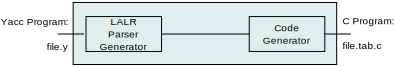
\includegraphics[width=.8\linewidth]{parser_tool}
	\end{center}
\end{frame}

\subsection{Yacc/Bison}

\tableofcontentslide[sectionstyle={show/shaded},subsectionstyle={show/shaded/hide},subsubsectionstyle={show/show/hide/hide}]

\subsubsection{Using Yacc/Bison}

\figureslide{Process of Yacc}{yacc_process}

\begin{frame}[t,fragile]{Structure of a Yacc Program}
	\begin{itemize}
	\item A Yacc program has the following form:
		\begin{lstlisting}[language=C]
		Declarations
		%%
		Translation rules
		%%
		Auxiliary functions
		\end{lstlisting}
	\end{itemize}
	\begin{small}
	\only<1>{\begin{block}{Declarations}
		\begin{itemize}
		\item C ordinary declarations, between \code{\%\{} and \code{\%\}}.
		\item Declarations of tokens with the command \code{\%token}.
		\end{itemize}
	\end{block}}
	\only<2>{\begin{block}{Translation rules}
		Each rule consists of a grammar production and the associated action (note the final semicolon).
		\begin{tabular}{@{}lcl@{}}
		{\textless}head{\textgreater}&:&{\textless}body$_1${\textgreater} \{ {\textless}action$_1${\textgreater} \} \\
		&$|$&{\textless}body$_2${\textgreater} \{ {\textless}action$_2${\textgreater} \} \\
		&&\dots \\
		&$|$&{\textless}body$_n${\textgreater} \{ {\textless}action$_n${\textgreater} \} \\
		&;&
		\end{tabular}
	\end{block}}
	\only<3>{\begin{block}{Auxiliary functions}
		\begin{itemize}
		\item Auxiliary functions are the section where additional C routines should be put.
		\item Note that you must provide the function \code{yylex()}, which is invoking the lexical analyzer (explained later).
		\end{itemize}
	\end{block}}
	\end{small}
\end{frame}

\begin{frame}[fragile]{Example of a Yacc Program}
	\begin{lstlisting}[language=C]
	%{
	    #include <ctype.h>
	%}
	%token DIGIT
	%%
	line   :   expr '\n'        { printf("%d\n", $1); }
	         ;
	expr   :   expr '+' term    { $$ = $1 + $3; }
	         | term
	         ;
	term   :   term '*' factor  { $$ = $1 * $3; }
	         | factor
	         ;
	factor :   '(' expr ')'     { $$ = $2; }
	         | DIGIT
	         ;
	%%
	int yylex() {
	   int c;
	   c = getchar();
	   if (isdigit(c)) {
	      yylval = c - '0'; /* convert char to int */
	      return DIGIT;
	   }
	   return c;
	}
	\end{lstlisting}
\end{frame}

\subsubsection{Ambiguous grammar}

\tableofcontentslide[sectionstyle={show/shaded},subsectionstyle={show/shaded/hide},subsubsectionstyle={show/shaded/hide/hide}]

\begin{frame}{Special Yacc Operators}
	\begin{itemize}
	\item Yacc provides a set of declarations that may be used to remove grammar ambiguity.
	\vfill
	\item Associativity and Precedence:
		\begin{description}
		\item[Left associativity] \%left {\textless}op1{\textgreater} {\textless}op2{\textgreater}\dots
		\item[Right associativity] \%right {\textless}op3{\textgreater} {\textless}op4{\textgreater}\dots
		\item[No associativity] \%nonassoc {\textless}op5{\textgreater} {\textless}op6{\textgreater}\dots
		\item The tokens are given precedences in the order in which they appear in  the declaration part, lower first.
		\item Tokens in the same declaration have the same precedence.
		\end{description}
	\end{itemize}
\end{frame}

\subsubsection{Connecting to Lex}

\tableofcontentslide[sectionstyle={show/shaded},subsectionstyle={show/shaded/hide},subsubsectionstyle={show/shaded/hide/hide}]

\begin{frame}{Use Lex in Conjonction with Yacc}
	\begin{itemize}
	\item Lex was designed to produce lexical analyzers that could be used with Yacc.
	\vfill
	\item The Lex library provides a driver program named \code{yylex()}.
	\vfill
	\item To use Lex in Yacc, you must remove any definition of \code{yylex() }in the Yacc specification; and replace this definition by:
		\begin{center}
		\texttt{\#include \str{"lex.yy.c"}}
		\end{center}
	\vfill
	\item All the tokens defined in the Yacc declaractions are directly available in the Lex program.
	\end{itemize}
\end{frame}

\subsubsection{Error recovery}

\tableofcontentslide[sectionstyle={show/shaded},subsectionstyle={show/shaded/hide},subsubsectionstyle={show/shaded/hide/hide}]

\begin{frame}{Error Production}
	\begin{itemize}
	\item In Yacc, error recovery uses a form of error productions.
	\item First, you must decides what ``major'' nonterminals will have error recovery associated to them.
	\item Typical choices are some subset of the nonterminals generating expressions, statements, blocks, and functions.
%	\item You then add to the grammar error productions of the form: \bnftext{A \bnfbody \tok{error} $\alpha$}, where $A$ is a major nonterminal and $\alpha$ is a string of grammar symbols, perhaps the empty string.
%	\item \tok{error} is a reserved word of Yacc.
	\end{itemize}
%	\begin{example}
%	The following production means that the parser skips just beyond the next semicolon on seeing an error.\\
%	\bnftext{stmt \bnfbody \tok{error}}
%	\end{example}
\end{frame}

\begin{frame}[fragile]{Error Recovery Functions}
	\begin{itemize}
	\item \code{yyerror()} reports an error.
	\item \code{yyerrok()} resets the parser to its normal mode of operation.
	\vfill
	\item \small Here, the error production causes the program to suspend normal parsing when a syntax error is found on an input line.
	\item \small On encountering the error, the parser in the program starts popping symbols from its stack until it encounters a statethat as a shift action on the token error. Then the input is read until the new-line character is read. Then the parser reduces error '{\textbackslash}n' to lines, and emits the diagnotic message ``error message.''
	\end{itemize}
	\begin{lstlisting}[language=C]
	line   :   lines expr '\n'  { printf("%g\n", $2); }
	         | lines '\n'
	         | /* empty or epsilon */
	         | error '\n'       { yyerror("error message");
                                      yyerrok(); }
	\end{lstlisting}
\end{frame}

\subsection{JavaCC}

\tableofcontentslide[sectionstyle={show/shaded},subsectionstyle={show/shaded/hide},subsubsectionstyle={show/show/hide/hide}]

\subsubsection{Using to JavaCC}

\figureslide{Process of JavaCC}{javacc_process}

\begin{frame}[t,fragile]{Structure of a JavaCC Program}
	\begin{itemize}
	\item A JavaCC program has the following form:
		\begin{lstlisting}[language=Java]
		JavaCC options
		PARSER_BEGIN(<parserName>)
		Java compilation unit
		PARSER_END(<parserName>)
		Translation rules
		\end{lstlisting}
	\end{itemize}
	\begin{small}
	\only<1>{\begin{block}{Parser Definition}
		\begin{itemize}
		\item The name that follows ``PARSER\_BEGIN'' and ``PARSER\_END'' must be the same and this identifies the name of the generated parser.
		\end{itemize}
	\end{block}}
	\only<2>{\begin{block}{Options}
		\begin{itemize}
		\item JavaCC options permits to control the behavior of the parser.
		\end{itemize}
	\end{block}}
	\only<3>{\begin{block}{Translation rules}
		The Java compilation unit is a Java code that must contain at least the declaration of the class of the parser: \\
		\dots \\
		\code{\tok{public} \tok{class} {\textless}parser\_name{\textgreater} \{} \\
		\dots \\
		\code{\}} \\
		\dots
	\end{block}}
	\only<4>{\begin{block}{Predefined functions}
		Two functions are automatically generated inside the parser class:
		\begin{itemize}
		\item \code{Token getNextToken()}: returns the next available token.
		\item \code{Token getToken(\tok{int} index)}: returns the ith token ahead.
		\end{itemize}
	\end{block}}
	\only<5>{\begin{block}{Translation rules}
		\begin{itemize}
		\item Java code production (see error recovery for an example),
		\item Regular expression production,
		\item BNF production, or
		\item Token manager declarations (not treated in this lecture).
		\end{itemize}
	\end{block}}
	\end{small}
\end{frame}

\begin{frame}{Define the Regular Expression Productions}
	\begin{definition}
		\code{[{\textless}state\_list{\textgreater}] {\textless}kind{\textgreater} [\tok{IGNORE\_CASE}] \tok{:}} \\
		\code{\{ {\textless}regexpr{\textgreater} $|$ {\textless}regexpr{\textgreater} $|$ \dots \}}
	\end{definition}
	\begin{itemize}
	\item \code{{\textless}state\_list{\textgreater}} specifies the lexer states in which the rule is enabled (default is \code{DEFAULT}).
	\item \tok{IGNORE\_CASE} specifies, by its presence, that if the regular expression is case sensitive or case insensitive.
	\item The regular definitions are defined and used as follows, respectively (The \code{"\#"} before the id indicates that this definition exists solely for the purpose of defining other tokens): \\
		\tok{\textless} [\tok{\#}]id \tok{:} regexpr \tok{\textgreater} \\
		\tok{\textless}id\tok{\textgreater}
	\end{itemize}
\end{frame}

\begin{frame}{Types of Regular Expression Productions \code{{\textless}kind{\textgreater}}}
	\begin{enumerate}
	\item[TOKEN] describes tokens in the grammar. The token manager creates a Token object for each match of such a regular expression and returns it to the parser.
	\vfill
	\item[SPECIAL\_TOKEN] like tokens, except that they do not have significance during parsing, ie. the BNF productions ignore them.
	\vfill
	\item[SKIP] simply skipped (ignored) by the token manager.
	\vfill
	\item[MORE] Sometimes it is useful to gradually build up a token to be passed on to the parser. Matches to this kind of regular expression are stored in a buffer until the next \tok{TOKEN} or \tok{SPECIAL\_TOKEN} match.
	\end{enumerate}
\end{frame}

\begin{frame}{Attributes of the Predefined \code{Token} Class}
	\begin{itemize}
	\item \code{\tok{int} kind} \\
		This is the index for this kind of token in the internal representation scheme of JavaCC. It may be replaced by a constant.
	\vfill
	\item \code{\tok{int} beginLine, beginColumn, endLine, endColumn} \\
		The beginning and ending positions of the token as it appeared in the input stream.
	\vfill
	\item \code{\tok{String} image} \\
		The image of the token as it appeared in the input stream.
	\vfill
	\item \code{\tok{Token} next} \\
		A reference to the next regular (non-special) token from the input stream.
	\end{itemize}
\end{frame}

\begin{frame}{Methods of the Predefined \code{Token} Class}
	\begin{itemize}
	\item \code{\tok{Object} getValue()} \\
		An optional attribute value of the \code{Token}. Tokens which are not used as syntactic sugar will often contain meaningful values that will be used later on by the compiler or interpreter. This attribute value is often different from the image. Any subclass of Token that actually wants to return a non-null value can override this method as appropriate.
	\vfill
	\item \code{\tok{static} \tok{final} Token newToken(\tok{int} ofKind)} \\
		\code{\tok{static} \tok{final} Token newToken(\tok{int} ofKind, \tok{String} image)} \\
		Returns a new token object as its default behavior.
	\end{itemize}
\end{frame}

\begin{frame}[t]{BNF Productions}
	\begin{definition}\small
		\code{{\textless}access\_modifier{\textgreater} {\textless}return\_type{\textgreater}} \\
		\code{{\textless}identifier{\textgreater} \tok( {\textless}parameters{\textgreater} \tok) \tok:} \\
		\code{{\textless}java\_block{\textgreater}} \\
		\code{\tok\{ {\textless}expansion\_choices{\textgreater} \tok\}}
	\end{definition}
	\begin{itemize}
	\item The name of the non-terminal is the name of the method, and the parameters and return value declared are the means to pass values up and down the parse tree.
	\item Non-terminals on the right hand sides of productions are written as method calls, so the passing of values up and down the tree are done using exactly the same paradigm as method call and return.
	\item The default access modifier for BNF productions is public.
	\end{itemize}
\end{frame}

\begin{frame}[t]{Heads of the Productions}
	\begin{definition}\small
		\code{{\textless}access\_modifier{\textgreater} {\textless}return\_type{\textgreater}} \\
		\code{{\textless}identifier{\textgreater} \tok( {\textless}parameters{\textgreater} \tok) \tok:} \\
		\code{{\textless}java\_block{\textgreater}} \\
		\code{\tok\{ {\textless}expansion\_choices{\textgreater} \tok\}}
	\end{definition}
	\begin{itemize}
	\item The name of the non-terminal is the name of the method, and the parameters and return value declared are the means to pass values up and down the parse tree.
	\item Non-terminals on the right hand sides of productions are written as method calls, so the passing of values up and down the tree are done using exactly the same paradigm as method call and return.
	\item The default access modifier for BNF productions is public.
	\end{itemize}
\end{frame}

\begin{frame}[t]{Bodies of the Productions}
	\begin{definition}\small
		\code{{\textless}access\_modifier{\textgreater} {\textless}return\_type{\textgreater}} \\
		\code{{\textless}identifier{\textgreater} \tok( {\textless}parameters{\textgreater} \tok) \tok:} \\
		\code{{\textless}java\_block{\textgreater}} \\
		\code{\tok\{ {\textless}expansion\_choices{\textgreater} \tok\}}
	\end{definition}
	\begin{description}
	\item[Java block] arbitrary Java declarations and code put at the beginning of the method generated for the Java non-terminal.
	\item[Expansion choices] a sequence of expansion units. Each nonterminal is written as a function call. Semantic actions are Java blocks inside this part of the BNF production.
	\end{description}
\end{frame}

\begin{frame}[fragile]{Example of JavaCC File \insertcontinuationwith{1}}
	\begin{lstlisting}{language=Java}
	PARSER_BEGIN(CalculatorParser)
	    public class CalculatorParser {
	    }
	PARSER_END(CalculatorParser)

	SKIP: {
	       " "
	    |  "\t"
	    |  "\n"
	    |  "\r"
	}

	TOKEN :
	{
	     <DIGIT : [0-9]>
	}
	\end{lstlisting}
\end{frame}

\begin{frame}[fragile]{Example of JavaCC File \insertcontinuationwith{2}}
	\begin{lstlisting}{language=Java}
	private void line() :
	{
	    int e;
	}
	{ e = expr()       { System.out.println(e); }
	}

	private int expr() :
	{
	    int e, t;
	}
	{ e = expr() "+" t = term()   { return e+t; }
	  | t = term()                { return v; }
	}
	\end{lstlisting}
\end{frame}

\begin{frame}[fragile]{Example of JavaCC File \insertcontinuationwith{3}}
	\begin{lstlisting}{language=Java}
	private int term() :
	{
	    int t, f;
	}
	{ t = term() "*" f = factor()   { return t*f; }
	  | f = factor()                { return f; }
	}

	private int factor() :
	{
	    int e, d;
	}
	{ "(" e = expr() ")"            { return e; }
	  | d = <DIGIT>                 { return Integer.parseInt(d.image); }
	}
	\end{lstlisting}
\end{frame}

\subsubsection{Error recovery}

\tableofcontentslide[sectionstyle={show/shaded},subsectionstyle={show/shaded/hide},subsubsectionstyle={show/shaded/hide/hide}]

\begin{frame}{Error Reporting with JavaCC}
	\begin{itemize}
	\item Simply modify the file \texttt{ParseException.java} to do what you want it to do. Typically, you would modify the \code{getMessage} method to do your own customized error reporting.
	\item All information regarding these methods can be obtained from the comments in the generated files \texttt{ParseException.java} and \texttt{TokenMgrError.java}.
	\vfill
	\item There is a method in the generated parser called \code{generateParseException()}.
	\item You can call this method anytime you wish to generate an object of type \code{ParseException}. This object will contain all the choices that the parser has attempted since the last successfully consumed token.
	\end{itemize}
\end{frame}

\begin{frame}{Error Recovery with JavaCC}
	JavaCC offers two kinds of error recovery:
	\vfill
	\begin{enumerate}
	\item[Shallow recovery] recovers if none of the current choices have succeeded in being selected.
	\vfill
	\item[Deep recovery] is when a choice is selected, but then an error happens sometime during the parsing of this choice.
	\end{enumerate}
\end{frame}

\begin{frame}[fragile]{Shallow Error Recovery}
	When no token found, we want to skip until the next given symbol (semi-column). \\
	\begin{lstlisting}{language=Java}
	TOKEN : { <SEMICOLON: ";"> }
	private void stm() :
	{}
	{ ifStm()
	  | whileStm()
	}
	\end{lstlisting}
	\begin{center}
\includegraphics[height=2em]{bottomarrow}\end{center}
	\begin{lstlisting}{language=Java}
	TOKEN : { <SEMICOLON: ";"> }
	private void stm() :
	{}
	{ ifStm()
	  | whileStm()
	  | whileStm()
	  | error_skipto(SEMICOLON)
	}
	\end{lstlisting}
\end{frame}

\begin{frame}[fragile]{Definition of the function \code{error\_skipto()}}
	\begin{itemize}
	\item \code{error\_skipto()} is a nonterminal that must be define prior to its first usage.
	\item To do so, we must use the following JAVACODE rule.
	\end{itemize}
	\begin{lstlisting}{language=Java}
	JAVACODE
	void error_skipto(int kind) {
	    ParseException e = generateParseException()
	    System.err.println(e);
	    Token t;
	    do {
	        t = getNextToken();
	    }
	    while (t.kind != kind);
	}
	\end{lstlisting}
\end{frame}

\begin{frame}[fragile]{Deep Error Recovery}
	When error occured (even deeper in the parse tree), we want to recover. \\
	\begin{lstlisting}{language=Java}
	TOKEN : { <SEMICOLON: ";"> }
	private void stm() :
	{}
	{ ifStm()
	  | whileStm()
	}
	\end{lstlisting}
	\mbox{}\hfill
\includegraphics[height=2em]{bottomarrow}\hfill\mbox{}
	\begin{lstlisting}{language=Java}
	TOKEN : { <SEMICOLON: ";"> }
	private void stm() :
	{}
	{ try {
	      ifStm()
	      | whileStm()
	      | whileStm()
	  } catch(ParseException e) {
	      error_skipto(e, SEMICOLON);
	  }
	}
	\end{lstlisting}
\end{frame}

\begin{frame}[fragile]{Definition of the function \code{error\_skipto()}}
	\begin{lstlisting}{language=Java}
	JAVACODE
	void error_skipto(ParseException e, int kind) {
	    System.out.println(e);
	    Token t;
	    do {
	        t = getNextToken();
	    }
	    while (t.kind != kind);
	}
	\end{lstlisting}
\end{frame}

\section{Conclusion}

\tableofcontentslide[sectionstyle={show/shaded},subsectionstyle={hide/hide/hide},subsubsectionstyle={hide/hide/hide/hide}]

\begin{frame}[t,allowframebreaks]{Key Concepts in the Chapter}
	\begin{small}
	\begin{description}
	\item[Parsers] A parser takes as input tokens from the lexical analyzer and treats the token names as terminal symbols of a context-free grammar. The parser then constructs a parse tree for its input sequence of tokens; the parse tree may be constructed figuratively or literally.
	\item[Context-Free Grammars] A grammar specifies a set of terminal symbols (inputs), another set of nonterminals (symbols representing syntactic constructs), and a set of productions, each of which gives a way in which strings represented by one nonterminal can be constructed from terminal symbols and strings represented by certain other nonterminals. A production consists of a head (the nonterminal to be replaced) and a body (the replacing string of grammar symbols).
	\item[Derivations] The process of starting with the start-nonterminal of a grammar and successively replacing it by the body of one its productions is called derivation. If the leftmost (or rightmost) nonterminal is always replaced, then the derivation is called leftmost (resp. rightmost.)
	\item[Parse Trees] A parse tree is a picture of a derivation, in which there is a node for each nonterminal that appears in the derivation. The children of a node are the symbols by which that nonterminal is replaced in the derivation. There is a one-to-one correspondence between parse trees, leftmost derivation, and rightmost derivations of the same terminal string.
	\item[Ambiguity] A grammar for which some terminal string has two or more different parse tree is said to be ambiguous.
	\item[Top-Down and Bottom-Up Parsing] Parsers are generally distinguished by whether they work top-down or bottom-up. Top-down parsers include recursive-descent and LL parsers, while the most common forms of bottom-up parsers are LR parsers.
	\item[Design of Grammars] Grammars suitable for top-down parsing often are harder to design than those used by bottom-up parsers. It is necessary to eliminate left-recursion. We also must left-factor/group productions for the same nonterminal that have a common prefix in the body.
	\item[Recursive-Descent Parsers] These parsers use a procedure for each nonterminal.
	\item[$LL(1)$ Parsers] A grammar such that it is possible to choose the correct production with which to expand a given nonterminal, looking only at the next input symbol, is called $LL(1)$. These grammars allow us to construct a predictive parsing table that gives, for each nonterminal and each lookahead symbol, the correct choice of production.
	\item[Shift-Reduce Parsing] Bottom-up parsers generally operate by choosing on the basis of the next input symbol and the contents of the stack, whether to shift the next input onto the stack, or to reduce some symbols at the top of the stack. A reduce takes a production body at the top of the stack and replaces it by the head of the production.
	\item[Viable Prefixes] In shift-reduce parsing, the stack contents are always a viable prefix, ie. a prefix of some right-sentential form that ends no further right than the end of the handle of that right-sentential form. The handler is the substring that was introduced in the last step of the rightmost derivation of that sentential form.
	\item[Valid Items] An item is a production with a dot somewhere in the body. An item is valid for a viable prefix if the production of that item is used to generate the handler, and the viable prefix includes all those symbols to the left of the dot.
	\item[$LR$ Parsers] Each of the several kinds of LR parsers operate by first constructing the sets of valid items (called LR states) for all possible viable prefixes, and keeping track of the state for each prefix on the stack. The set of valid items guide the shift-reduce parsing decision.
	\item[Simple $LR$ Parsers] In an $SLR$ parser, we perform a reduction implied by a valid item with a dot at the right end, provided the lookahead symbol can follow the head of that production in some sentential form.
	\item[Canonical-$LR$ Parsers] This more complex form of $LR$ parser uses items that are augmented by the set of lookahead symbols that can follow the use of the underlying production. A canonical-$LR$ parser can avoid some of the parsing-action conflicts that are present in $SLR$ parsers, but often has many more states than the $SLR$ parser for the same grammar.
	\end{description}
	\end{small}
\end{frame}

\begin{frame}[t,allowframebreaks]{\bibname\ of the Chapter}%
	\tiny%
	\putbib[bibliographies/chapter3]%
\end{frame}%

\end{bibunit}


%\setbeamertemplate{headline text style}{\Tiny}%

\begin{bibunit}[apalike]

\part[author={Stéphane GALLAND},label={chap:intermediate_code_generation}]{Intermediate Code Generation}

\tableofcontentslide

\section{Introduction}

\begin{frame}{Introduction}
	\vfill
	\begin{itemize}
	\item This chapter develops two major points:
		\vfill
		\begin{enumerate}
		\item The translation of languages guided by context-free grammars.
		\vfill
		\item These translation techniques are applied to type checking and intermediate code generation.
		\end{enumerate}
	\end{itemize}
	\vfill
	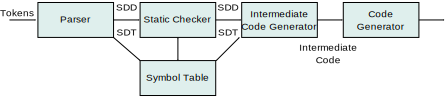
\includegraphics[width=\linewidth]{parser_toolchain}
\end{frame}

\sidecite{Samelson.1960, Brooker.1962}
\begin{frame}{Syntax-Directed Translation}
	\begin{itemize}
	\item A \emph{syntax-directed translation} specifies the values of attributes, attached to the grammar symbols, by associating semantic rules with the grammar productions.
		\begin{sdd}
		\p{expr ::= expr \tok+ term}{head.t = expr.t \concat term.t \concat '+'}
		\p{     ::= expr \tok- term}{head.t = expr.t \concat term.t \concat '-'}
		\p{     ::= term}{head.t = term.t}
		\p{term ::= \tok0}{head.t = '0'}
		\p{     ::= \tok1}{head.t = '1'}
		\pdots
		\p{     ::= \tok9}{head.t = '9'}
		\end{sdd}
	\vspace{1em}
	\item A Syntax-directed translation scheme embeds program fragments (or semantic actions, between braces) inside the semantic rules.
	\end{itemize}
\end{frame}

\begin{frame}{Two Types of Syntax-Directed Translation}
	\begin{itemize}
	\item The most general approach to syntax-directed translation is:
		\begin{itemize}
		\item to construct a parse tree, and
		\item then to compute the values of the attributes at the nodes of the tree by visiting the nodes.
		\end{itemize}
	\vfill
	\item In many cases, translation can be done during parsing, without building an explicit tree.
	\vfill
	\item Two classes of syntax-directed translation are presented:
		\begin{itemize}
		\item \emph{L-attributed translations} (L=left)
		\item \emph{S-attributed translations} (S=synthesized)
		\end{itemize}
	\end{itemize}
\end{frame}

\begin{frame}{Program Checking}
	\begin{itemize}
	\item Static checking includes \emph{type checking}, which ensures that operators are applied to compatible operands.
	\vspace{4em}
	\item It also includes any \emph{syntactic checks} that remain after parsing.
	\end{itemize}
\end{frame}

\begin{frame}{Intermediate Representation}
	\begin{itemize}
	\item In the process of translating a program in a given source language into code for a given target machine, a compiler may construct a sequence of intermediate representations. \\
	\vfill
		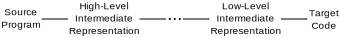
\includegraphics[width=\linewidth]{intermediate_representations}
	\vfill
	\item High-level representation is close to the source language \eg syntax tree.
	\item Low-level representation are close to the target machine \eg three-address code.
	\end{itemize}
\end{frame}

\section{Translation scheme}

\tableofcontentslide[sections={1-4},sectionstyle={show/shaded},subsectionstyle={show/show/hide},subsubsectionstyle={hide/hide/hide/hide}]

\subsection{Syntax-directed translation}

\sidecite{Paakki.1995}
\begin{frame}{Syntax-Directed Translation}
	\begin{definition}
		Syntax-directed translation is done by attaching rules or program fragments to productions in a grammar.
	\end{definition}
	\begin{itemize}
	\item The rules or program fragments are named ``semantic rules.''
	\item Each of these semantic rules permits to translate the source program into the target program. \\
		\inlineexample{Translate infix arithmetic expressions into postfix arithmetic expressions.}
	\end{itemize}
	\vfill
	\alertbox{Two concepts are related to syntax-directed translation: \emph{attributes} and \emph{translation schemes}}
\end{frame}

\subsection{Syntax-directed definition}

\tableofcontentslide[sections={1-4},sectionstyle={show/shaded},subsectionstyle={show/shaded/hide},subsubsectionstyle={show/show/hide/hide}]

\begin{frame}{Syntax-Directed Definition}
	\begin{definition}[Syntax-Directed Definition --- SDD]
		A context-free grammar together with attributes and rules.
	\end{definition}
	\begin{itemize}
	\item Attributes are associated with grammar symbols.
	\item Rules are associated with productions.
	\end{itemize}
	\vfill
	\begin{sdd}
	\ptitle{Productions}{Semantic Rules}
	\p{expr ::= expr \tok+ term}{head.t = expr.t \concat term.t \concat '+'}
	\p{     ::= expr \tok- term}{head.t = expr.t \concat term.t \concat '-'}
	\p{     ::= term}{head.t = term.t}
	\p{term ::= \tok0}{head.t = '0'}
	\p{     ::= \tok1}{head.t = '1'}
	\pdots
	\p{     ::= \tok9}{head.t = '9'}
	\end{sdd}
\end{frame}

\begin{frame}{Two Notations for Syntax-Directed Definition}
	\begin{itemize}
	\item Notation during the lectures:
		\begin{sdd}
		\ptitle{Productions}{Semantic Rules}
		\p{A ::= B C}{First part of Rule 1}
		\pcont{D E}{Second part of Rule 1}
		\p{  ::= F}{Rule 2}
		\p{G ::= H I J}{Rule 3}
		\end{sdd}
	\vfill
	\item Notation during the tutorial sessions and labworks:
		\begin{tabularx}{\linewidth}{|lcX|}
		\hline
		{\bnfstyle A} & $\rightarrow$ & {\bnfstyle B C} \texttt{\{ First part of Rule 1 \}} {\bnfstyle D E} \texttt{\{ Second part of Rule 1 \}} \\
		& $|$ & {\bnfstyle F} \texttt{\{ Rule 2 \}} \\
		{\bnfstyle G} & $\rightarrow$ & {\bnfstyle H I J} \texttt{\{ Rule 3 \}} \\
		\hline
		\end{tabularx}
	\end{itemize}
\end{frame}

\subsection{Attributes of the productions}

\tableofcontentslide[sections={1-4},sectionstyle={show/shaded},subsectionstyle={show/shaded/hide},subsubsectionstyle={show/show/hide/hide}]

\begin{frame}{Attributes}
	\begin{itemize}
	\item An \emph{attribute} is any quantity associated with a programming construct.
	\vfill
	\item \inlineexamples{data types, number of instructions, line of the first occurrence of an identifier\dots}
	\vfill
	\item Since we use grammar symbols (terminals and nonterminals) to represent programming constructs, we extend the notion of attributes from constructs to the symbols that represent them.
	\end{itemize}
\end{frame}

\begin{frame}{Notation for Attributes}
	\begin{itemize}
	\item In this lecture, the attributes are written as one of:
		\begin{itemize}
		\item \texttt{{\textless}terminal{\textgreater}.{\textless}attribute name{\textgreater}}; or
		\item \texttt{{\textless}nonterminal{\textgreater}.{\textless}attribute name{\textgreater}}.
		\end{itemize}
	\item The keyword \texttt{head} represents the nonterminal in the head of the rule.
	\item If the same nonterminal is present many times in the same rule body, the attribute prefix is indexed by the position of the nonterminal in this body.
	\end{itemize}
	\vfill
	\begin{sdd}
	\p{\protect\textcolor{IRTESmagenta}{expr} ::= expr \tok+ expr}{\textcolor{IRTESmagenta}{head.t} = expr$_1$.t \concat expr$_2$.t \concat '+'}
	\p{     ::= \textcolor{IRTESgreen}{expr} \tok- expr}{head.t = \textcolor{IRTESgreen}{expr$_1$.t} \concat expr$_2$.t \concat '-'}
	\p{     ::= \textcolor{IRTESblue}{term}}{head.t = \textcolor{IRTESblue}{term.t}}
	\p{term ::= \tok0}{head.t = '0'}
	\p{     ::= \tok1}{head.t = '1'}
	\pdots
	\p{     ::= \tok9}{head.t = '9'}
	\end{sdd}
\end{frame}

\begin{frame}{Synthetized Attribute}
	\begin{definition}
		A \emph{synthesized attribute} for a nonterminal $A$ at a parse-tree node $N$ is defined by a semantic rule associated with the production at $N$.
	\end{definition}
	\vfill
	\begin{itemize}
	\item Note that the production must have $A$ as its head.
	\vfill
	\item A synthesized attribute at node $N$ is defined only in terms of attribute values at the children of $N$ and at $N$ itself.
	\end{itemize}
\end{frame}

\sidecite{Knuth.1968}
\begin{frame}{Inherited Attribute}
	\begin{definition}
		An \emph{inherited attribute} for a nonterminal $B$ at a parse-tree node $N$ is defined by a semantic rule associated with the production at the parent of $N$.
	\end{definition}
	\vfill
	\begin{itemize}
	\item Note that the production must have $B$ as a symbol in its body. 
	\vfill
	\item An inherited attribute at node $N$ is defined only in terms of attribute values at $N$'s parent, $N$ itself, and $N$'s siblings.
	\end{itemize}
\end{frame}

\subsection{Evaluating a SDD with a parse tree}

\tableofcontentslide[sections={1-4},sectionstyle={show/shaded},subsectionstyle={show/shaded/hide},subsubsectionstyle={show/show/hide/hide}]

\begin{frame}{Evaluating a SDD with a Parse Tree}
	\alertbox*{To visualize the translation specified by an SDD, it helps to work with parse trees}
	\vfill
	\begin{itemize}
	\item A parse tree, showing the value(s) of its attribute(s) is called an \emph{annotated parse tree}.
	\vfill
	\item Before we can evaluate an attribute at a node of a parse tree, we must evaluate all the attributes upon which its value depends.
	\vfill
	\item With synthesized attributes, we can evaluate attributes in any bottom-up order, such that of a postorder traversal of the parse tree.
	\end{itemize}
\end{frame}

\pgfdeclareimage[width=3em]{leftarrow}{imgs/all/leftarrow}

\begin{frame}[t]{Example of Evaluation}
	\begin{center}
		\begin{small}
		\begin{sdd}[.7\linewidth]
		\p{T  ::= F T'}{	T'.lval = F.val \newl
					head.val = T'.val}
		\p{T' ::= \tok* F T'}{	T'.lval = head.lval * F.val \newl
					head.val = T'.val}
		\p{   ::= $\epsilon$}{	head.val = head.lval}
		\p{F  ::= \tok{digit}}{	head.val = \tok{digit}.lexval}
		\end{sdd}
		\end{small} \\[1em]
		Input: \texttt{3 * 5}
	\end{center}
	\putat(50,-215){\includeanimatedfigure[height=.4\paperheight]{sdd_evaluation}}
	\only<5,10>{\putat(245,-89){\pgfuseimage{leftarrow}}}
	\only<6>{\putat(228,-40){\pgfuseimage{leftarrow}}}
	\only<11>{\putat(258,-60){\pgfuseimage{leftarrow}}}
	\only<12>{\putat(245,-79){\pgfuseimage{leftarrow}}}
	\only<13>{\putat(245,-70){\pgfuseimage{leftarrow}}}
	\only<14>{\putat(235,-50){\pgfuseimage{leftarrow}}}
\end{frame}

\begin{frame}{Problem of the Evaluation Order}
	\alertbox{How to determine the correct sequence of evaluations of the semantic rules' lines?}
	\vspace{4em}
	\alertbox*{Introduction of a \Emph{graph of dependencies} between the attributes.}
\end{frame}

\subsection{Dependency graph}

\tableofcontentslide[sections={1-4},sectionstyle={show/shaded},subsectionstyle={show/shaded/hide},subsubsectionstyle={show/show/hide/hide}]

\sidecite{Knuth.1968}
\begin{frame}{Dependency Graph}
	\begin{definition}
		A \emph{dependency graph} depicts the flow of information among the attribute instances in a particular parse tree.
	\end{definition}
	\vfill
	\begin{description}
	\item[Node] For each parse-tree node, say a node labeled by grammar symbol $X$, the dependency graph has a node for each attribute associated with $X$.
	\item[Edge] Between two attribute instances. Means that the value of the first is needed to compute the second.
	\end{description}
\end{frame}

\begin{frame}[t]{Examples of Atomic Dependency Graphs}
	\begin{center}
		\begin{small}
		\begin{sdd}[.7\linewidth]
		\p{T  ::= F T'}{	T'.lval = F.val \newl
					head.val = T'.val}
		\p{T' ::= \tok* F T'}{	T'.lval = head.lval * F.val \newl
					head.val = T'.val}
		\p{   ::= $\epsilon$}{	head.val = head.lval}
		\p{F  ::= \tok{digit}}{	head.val = \tok{digit}.lexval}
		\end{sdd}
		\end{small}
	\end{center}
	\putat(0,-160){\includeanimatedfigure[width=\linewidth]{dependency_graph_example}}
\end{frame}

\begin{frame}[t]{Examples of Dependency Graph on Input}
	\begin{center}
		\begin{small}
		\begin{sdd}[.7\linewidth]
		\p{T  ::= F T'}{	T'.lval = F.val \newl
					head.val = T'.val}
		\p{T' ::= \tok* F T'}{	T'.lval = head.lval * F.val \newl
					head.val = T'.val}
		\p{   ::= $\epsilon$}{	head.val = head.lval}
		\p{F  ::= \tok{digit}}{	head.val = \tok{digit}.lexval}
		\end{sdd}
		\end{small} \\[1em]
		Input: \texttt{3 * 5}
	\end{center}
	\putat(80,-210){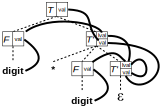
\includegraphics[width=.5\linewidth]{dependency_graph_example2}}
\end{frame}

\sidecite{Knuth.1968}
\begin{frame}{Order of the Attributes}
	\begin{itemize}
	\item The dependency graph characterizes the possible orders in which we can evaluate the attributes at the various nodes of a parse tree.
	\vfill
	\item If the dependency graph has an edge from node $M$ to node $N$, then the attribute corresponding to $M$ must be evaluated before the attribute of $N$.
	\vfill
	\item The only allowable orders of evaluation are those sequences of nodes $N_1, N_2, \dots, N_k$ such that if there is an edge of the dependency graph from $N_i$ to $N_j$, then $i<j$.
	\vfill
	\item Such an ordering embeds a directed graph into a linear order, and is called a topological sort of the graph.
	\end{itemize}
\end{frame}

\sidecite{Knuth.1968, Jazayeri.1975}
\begin{frame}{Problem to Determine the Order of the Attributes}
	\alertbox{If there is any cycle in the graph, then there are no topological sorts; ie. there is no way to evaluate the SDD on the parse tree.}
	\vfill
	\alertbox{Given a SDD, it is very hard to tell whether there exist any parse trees whose dependency graphs have cycles.}
	\vfill
	\begin{itemize}
	\item Translations can be implemented using classes of SDD that guarantee an evaluation order, ie. without cycle.
	\vfill
	\item Two possible approaches to solve this problem:
		\begin{enumerate}
		\item  S-attributed definition.
		\item L-attributed definition.
		\end{enumerate}
	\end{itemize}
\end{frame}

\subsection{S-attributed definition}

\tableofcontentslide[sections={1-4},sectionstyle={show/shaded},subsectionstyle={show/shaded/hide},subsubsectionstyle={show/show/hide/hide}]

\sidecite{Irons.1961}
\begin{frame}{S-Attributed Definition}
	\begin{definition}
		An S-attributed definition is an SDD in which all the attributes are synthesized.
	\end{definition}
	\vspace{4em}
	\begin{itemize}
	\item S-attributed definitions can be implemented during bottom-up parsing, since a bottom-up parse corresponds to a postorder traversal of the parse tree.
	\end{itemize}
\end{frame}

\subsection{L-attributed definition}

\tableofcontentslide[sections={1-4},sectionstyle={show/shaded},subsectionstyle={show/shaded/hide},subsubsectionstyle={show/show/hide/hide}]

\sidecite{Lewis.1974}
\begin{frame}{L-Attributed Definition}
	\begin{footnotesize}
	\begin{definition}
		An L-attributed definition is an SDD in which, between the attributes associated with a production body, dependency-graph edges can go from left to right, but not from right to left.
	\end{definition}
	Each attribute must be:
	\begin{itemize}
	\item Synthesized, or
	\item Inherited, with the rules limited as follows. \\
		Suppose a production \bnftext{A \bnfbody $X_1 X_2 \dots X_n$}, and an inherited attribute $X_i.a$. The rule may uses only:
		\begin{enumerate}[a)]\footnotesize
		\item Inherited attributes associated with the head $A$.
		\item Either inherited or synthesized attributes associated with the occurrences of symbols $X_1 X_2 \dots X_{i-1}$ located to the left of $X_i$.
		\item Inherited or synthesized attributes associated with this occurrence of $X_i$ itself, but only in such a way that there are no cycles in a graph dependency formed by the attributes of this $X$.
		\end{enumerate}
	\end{itemize}
	\end{footnotesize}
\end{frame}

\section{Syntax tree and graph}

\tableofcontentslide[sections={1-6},sectionstyle={show/shaded},subsectionstyle={show/show/hide},subsubsectionstyle={hide/hide/hide/hide}]

\subsection{Syntax tree}

\subsubsection{Definition}

\tableofcontentslide[sections={1-5},sectionstyle={show/shaded},subsectionstyle={show/shaded/hide},subsubsectionstyle={show/show/hide/hide}]

\begin{frame}{Syntax Tree as Intermediate Representation}
	\begin{itemize}
	\item Since some compilers use \emph{syntax tree as an intermediate representation}, a common form of SDD turns its input string into a tree.
	\vfill
	\item To complete the translation to intermediate code, the compiler may then walk the syntax tree, using another set of rules that are in effect an SDD on the syntax tree rather than the parse tree.
	\vfill
	\item Two SDD are considered in this section to build a syntax tree:
		\begin{itemize}
		\item S-attributed definition (bottom-up), and
		\item L-attributed definition (top-down).
		\end{itemize}
	\end{itemize}
\end{frame}

\begin{frame}{Syntax Tree}
	\begin{itemize}
	\item \Emph{Each node in a syntax tree represents a language construct.}
	\item The children of the node represent the meaningful components of the construct.
	\vfill
	\item We shall implement the nodes of a syntax tree by objects with a suitable number of fields.
	\vfill
	\item Each object will have an operator field that is the label of the node, and the following additional fields:
		\begin{itemize}
		\item If the node is a leaf, the lexical value for the leaf.
		\item If the node is an interior node, all the children are stored in individual fields.
		\end{itemize}
	\end{itemize}
\end{frame}

\begin{frame}{Example of a Syntax Tree}
	\begin{center}
		This is the syntax tree for the statement: \\
			\texttt{a := 3 + ( 6 * 7 )} \\[2em]
		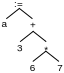
\includegraphics[width=.2\linewidth]{syntax_tree_example2}
	\end{center}
\end{frame}

\subsubsection{Building from S-attributed definition}

\tableofcontentslide[sections={1-5},sectionstyle={show/shaded},subsectionstyle={show/shaded/hide},subsubsectionstyle={show/shaded/hide/hide}]

\begin{frame}[t]{S-Attributed Definition for Building a Syntax Tree}
	\begin{small}
	\begin{center}
		\begin{sdd}[.9\linewidth]
		\p{E ::= E \tok+ T}{head.node = \kw{new} Node(\str{"+"}, E.node, T.node)}
		\p{  ::= E \tok- T}{head.node = \kw{new} Node(\str{"-"}, E.node, T.node)}
		\p{  ::= T}{head.node = T.node}
		\p{T ::= \tok( E \tok)}{head.node = E.node}
		\p{  ::= \tok{id}}{head.node = \kw{new} Leaf(\tok{id}, \tok{id}.lexeme)}
		\p{  ::= \tok{num}}{head.node = \kw{new} Leaf(\tok{num}, \tok{num}.value)}
		\end{sdd}
	\end{center}
	\vspace{2em}
	\begin{itemize}
	\item The semantic rules contain the creation of the syntax tree nodes, with the description of the node and/or the children as parameters. The root of the syntax tree becomes \texttt{E.node}.
	\item Note that the annotated parse tree is implicitly defined by the grammar rules and not directly built by the compiler.
	\end{itemize}
	\end{small}
\end{frame}

\begin{frame}[t]{Example of Syntax Tree Building}
	\begin{small}
	\begin{center}
		\begin{sdd}[.9\linewidth]
		\p{E ::= E \tok+ T}{head.node = \kw{new} Node(\str{"+"}, E.node, T.node)}
		\p{  ::= E \tok- T}{head.node = \kw{new} Node(\str{"-"}, E.node, T.node)}
		\p{  ::= T}{head.node = T.node}
		\p{T ::= \tok( E \tok)}{head.node = E.node}
		\p{  ::= \tok{id}}{head.node = \kw{new} Leaf(\tok{id}, \tok{id}.lexeme)}
		\p{  ::= \tok{num}}{head.node = \kw{new} Leaf(\tok{num}, \tok{num}.value)}
		\end{sdd} \\[1em]
		Input: \texttt{a - 4 + c}
	\end{center}
	\end{small}
	\putat(10,-215){\includeanimatedfigure[height=.4\paperheight]{syntax_tree_sattr}}
	\only<9>{\putat(290,-40){\pgfuseimage{leftarrow}}}
	\only<7>{\putat(290,-50){\pgfuseimage{leftarrow}}}
	\only<5>{\putat(280,-58){\pgfuseimage{leftarrow}}}
	\only<3-4,8>{\putat(270,-79){\pgfuseimage{leftarrow}}}
	\only<6>{\putat(270,-89){\pgfuseimage{leftarrow}}}
\end{frame}

\subsubsection{Building from L-attributed definition}

\tableofcontentslide[sections={1-5},sectionstyle={show/shaded},subsectionstyle={show/shaded/hide},subsubsectionstyle={show/shaded/hide/hide}]

\begin{frame}[t]{L-Attributed Definition for Building a Syntax Tree}
	\begin{small}
	\begin{center}
		\begin{scriptsize}
		\begin{sdd}[.7\linewidth]
		\p{E  ::= T E'}{E'.left = T.node \newl
					head.node = E'.node}
		\p{E' ::= \tok+ T E'}{E'.parent = \kw{new} Node(\str{"+"}, head.left, T.node) \newl
					head.node = E'.node}
		\p{   ::= \tok- T E'}{E'.parent = \kw{new} Node(\str{"-"}, head.left, T.node) \newl
					head.node = E'.node}
		\p{   ::= $\epsilon$}{head.node = head.left}
		\p{T  ::= \tok( E \tok)}{head.node = E.node}
		\p{   ::= \tok{id}}{head.node = \kw{new} Leaf(\tok{id}, \tok{id}.lexeme)}
		\p{   ::= \tok{num}}{head.node = \kw{new} Leaf(\tok{num}, \tok{num}.value)}
		\end{sdd}
		\end{scriptsize}
	\end{center}
	\vspace{2em}
	\begin{itemize}
	\item Note that the annotated parse tree is implicitly defined by the grammar rules and not directly built by the compiler.
	\end{itemize}
	\end{small}
\end{frame}

\begin{frame}[t]{Example of Syntax Tree Building}
	\begin{small}
	\begin{center}
		\begin{scriptsize}
		\begin{sdd}[.7\linewidth]
		\p{E  ::= T E'}{E'.left = T.node \newl
					head.node = E'.node}
		\p{E' ::= \tok+ T E'}{E'.parent = \kw{new} Node(\str{"+"}, head.left, T.node) \newl
					head.node = E'.node}
		\p{   ::= \tok- T E'}{E'.parent = \kw{new} Node(\str{"-"}, head.left, T.node) \newl
					head.node = E'.node}
		\p{   ::= $\epsilon$}{head.node = head.left}
		\p{T  ::= \tok( E \tok)}{head.node = E.node}
		\p{   ::= \tok{id}}{head.node = \kw{new} Leaf(\tok{id}, \tok{id}.lexeme)}
		\p{   ::= \tok{num}}{head.node = \kw{new} Leaf(\tok{num}, \tok{num}.value)}
		\end{sdd}
		\end{scriptsize}\\[1em]
		Input: \texttt{a - 4 + c}
	\end{center}
	\end{small}
	\putat(-10,-215){\includeanimatedfigure[height=.35\paperheight]{syntax_tree_lattr}}
	\only<5>{\putat(258,-39){\pgfuseimage{leftarrow}}}
	\only<13>{\putat(258,-46){\pgfuseimage{leftarrow}}}
	\only<9>{\putat(258,-53){\pgfuseimage{leftarrow}}}
	\only<11>{\putat(258,-59){\pgfuseimage{leftarrow}}}
	\only<7>{\putat(258,-67){\pgfuseimage{leftarrow}}}
	\only<12>{\putat(258,-73){\pgfuseimage{leftarrow}}}
	\only<10>{\putat(258,-81){\pgfuseimage{leftarrow}}}
	\only<4,8>{\putat(258,-94){\pgfuseimage{leftarrow}}}
	\only<6>{\putat(258,-102){\pgfuseimage{leftarrow}}}
\end{frame}

\subsection{Directed acyclic graph}

\tableofcontentslide[sections={1-6},sectionstyle={show/shaded},subsectionstyle={show/shaded/hide},subsubsectionstyle={show/show/hide/hide}]

\begin{frame}{Directed Acyclic Graph}
	\begin{itemize}
	\item Nodes in a syntax tree represent language constructs in the source program; the children of a node represent the meaningful components of a construct.
	\end{itemize}
	\vfill
	\begin{definition}[Directed Acyclic Graph]
		A directed acyclic graph (DAG) represent the language constructs un the source program.
		It ensures that a construct is present only one time in the DAG.
	\end{definition}
	\vfill
	\begin{itemize}
	\item The difference between syntax tree and DAG is that the DAG node may have more than one parent.
	\item Consequently, a subexpression is repeated in a tree; and shared in a DAG.
	\end{itemize}
\end{frame}

\begin{frame}{Example of Directed Acyclic Graph}
	\begin{center}
		$a \tok+ a \tok* \tok( b \tok- c \tok) \tok+ \tok( b \tok- c \tok) \tok* d$
	\end{center}
	\vspace{2em}
	\includeanimatedfigure[width=\linewidth]{dag_example}
\end{frame}

\begin{frame}[fragile]{Value-Number Representation for the DAG}
	\begin{footnotesize}
	\begin{itemize}
	\item Often, the nodes of a DAG are stored in an array of records (also true for a syntax tree).
	\end{itemize}
	\begin{columns}
		\begin{column}{.2\linewidth}
			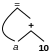
\includegraphics[width=\linewidth]{simple_dag}
		\end{column}
		\begin{column}{.4\linewidth}
			\begin{scriptsize}
			\begin{tabularx}{\linewidth}{|c|X|X|X|}
				\hline
				1 & \tok{id} & \multicolumn{2}{l|}{to symbol $a$} \\
				\hline
				2 & \tok{num} & \multicolumn{2}{l|}{10} \\
				\hline
				3 & \tok+ & 1 & 2 \\
				\hline
				4 & \tok= & 1 & 3 \\
				\hline
			\end{tabularx}
			\end{scriptsize}
		\end{column}
		\begin{column}{.4\linewidth}
			\begin{scriptsize}
			\begin{lstlisting}[language=C]
			struct {
			   int token_id;
			   union {
			      unsigned int symbol_index;
			      double fvalue;
			      long lvalue;
			      struct {
			         unsigned int left;
			         unsigned int right;
			      } operands;
			   } attr;
			} Record;
			\end{lstlisting}
			\end{scriptsize}
		\end{column}
	\end{columns}
	\begin{itemize}
	\item Each node of the DAG is referred by its index in the table; its \emph{value number}.
	\item Let the signature of an interior node be the triple $\langle op,l,r \rangle$, where $op$ is the label, $l$ its left child's value number, and $r$ its right child's value number. $l$ and $r$ are set to $0$ when there is no child.
	\end{itemize}
	\end{footnotesize}
\end{frame}

\begin{frame}[fragile]{Building a DAG}
	\begin{description}
	\item[INPUT] Label $op$, node $l$, and node $r$.
	\item[OUTPUT] The value number of a node in the array with signature $\langle op,l,r \rangle$.
	\vfill
	\item[METHOD] Search the array for a node $M$ with label $op$, left child $l$, and right child $r$. If there is such a node return the value number of $M$. If not, create in the array a new node $N$ with label $op$, left child $l$, right child $r$, and return its value number.
	\vfill
	\item[NOTE] This approach is searching the entire array every time; it is not efficient. A more efficient approach is to use a hash table, in which the nodes are put into ``buckets,'' each of which typically will have only few nodes.
	\end{description}
\end{frame}

\section{Three-address code}

\tableofcontentslide[sections={1-5},sectionstyle={show/shaded},subsectionstyle={show/show/hide},subsubsectionstyle={hide/hide/hide/hide}]

\sidecite{Strong.1958, Wirth.1971, Johnson.1979, Ritchie.1979}
\begin{frame}{Level of Intermediate Representation}
	\alertbox*{The syntax tree is a \Emph{high-level} intermediate representation of the source program.}
	\vspace{2em}
	\alertbox{To make easier the generation of low-level code, a low-level intermediate representation is useful.}
	\vspace{2em}
	\alertbox*{The \Emph{three-address code} is a form of low-level intermediate representation that is close to the assembler languages.}
	\begin{tiny}
		\alert{Note:} The rest of this lecture focuses on the generation of code with three-address code. The syntax tree may be also used as a basis of the generation (see the supervised tutorials).
	\end{tiny}
\end{frame}

\sidecite{Strong.1958, Gosling.1995}
\begin{frame}{What is Three-Address Code?}
	\begin{itemize}
	\item In three-address code, there is at most one operator on the right side of an instruction.
		\begin{center}
			\begin{tac}[.3\linewidth]
				\a{\t1}{y * z}
				\a{\t2}{x + \t2}
			\end{tac}
		\end{center}
	\item where \tactext{\t1} and \tactext{\t2} are  compiler-generated temporary names.
	\end{itemize}
	\begin{columns}
		\begin{column}{.3\linewidth}
			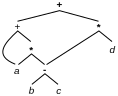
\includegraphics[width=\linewidth]{dag_alone_example}
		\end{column}
		\begin{column}{.5\linewidth}
			\begin{tac}[\linewidth]
				\a{\t1}{b - c}
				\a{\t2}{a * \t1}
				\a{\t3}{a + \t2}
				\a{\t4}{\t1 * d}
				\a{\t5}{\t3 + \t4}
			\end{tac}
		\end{column}
	\end{columns}
\end{frame}

\subsection{Language basics}

\begin{frame}{Address}
	An address can be one of the following:
	\begin{enumerate}
	\item[Name] For convenience, we allow source-program names to appear as addresses in three-address code. In an implementation, a source name is replaced by a pointer to its symbol-table entry, where all information about the name is kept.
	\vfill
	\item[Constant] A compiler must deal with many different types of constants and variables.
	\vfill
	\item[Compiler-generated temporary Name] It is useful, especially in optimizing compilers, to create a distinct name each time a temporary is needed. These temporaries can be combined, if possible, when registers are allocated to variables.
	\end{enumerate}
\end{frame}

\begin{frame}{Label}
	\begin{itemize}
	\item A symbolic label represents the index of a three-address instruction in the sequence of instructions.
	\item Numeric positions can be substituted for the labels, either by making a separate pass or by ``backpatching.''
	\end{itemize}
	\begin{columns}
		\begin{column}{.4\linewidth}
			\begin{center}
			\begin{tac}[\linewidth]
				\a[L]{\t1}{i + 1}
				\a{i}{\t1}
				\a{\t2}{i * 8}
				\a{\t3}{a [ \t2 ]}
				\ifgoto{\t3 $<$ v}{L}
			\end{tac} \\[1em]
			\emph{Symbolic Label}
			\end{center}
		\end{column}
		\begin{column}{.5\linewidth}
			\begin{center}
			\begin{tac}[\linewidth]
				\a[103]{\t1}{i + 1}
				\a[104]{i}{\t1}
				\a[105]{\t2}{i * 8}
				\a[106]{\t3}{a [ \t2 ]}
				\ifgoto[107]{\t3 $<$ v}{103}
			\end{tac} \\[1em]
			\emph{Numeric Position}
			\end{center}
		\end{column}
	\end{columns}
\end{frame}

\begin{frame}{Assignment Instruction}
	\begin{itemize}
	\item Assignment instruction of the form \emph{\tactext{x = y {\textless}op{\textgreater} z}}, where \tactext{{\textless}op{\textgreater}} is a binary arithmetic or logical operation, and \tactext{x}, \tactext{y}, and \tactext{z} are addresses.
	\vfill
	\item Assignment instruction of the form \emph{\tactext{x = {\textless}op{\textgreater} y}}, where \tactext{{\textless}op{\textgreater}} is an unary operation. Essential unary operations include unary minus, logical negation, and conversion operators.
	\vfill
	\item Copy instruction of the form \emph{\tactext{x = y}}, where \tactext{x} is assigned the value of \tactext{y}.
	\end{itemize}
\end{frame}

\begin{frame}{Jumping Instruction}
	\begin{itemize}
	\item An unconditional jump \emph{\tactext{\kw{goto} L}}. The three-address instruction with label \tactext{L} is the next executed.
	\vfill
	\item Conditional jumps of the form \emph{\tactext{\kw{if} x \kw{goto} L}}, and \emph{\tactext{\kw{ifFalse} x \kw{goto} L}}. These instructions execute the instruction with label \tactext{L} next if \tactext{x} is true and false, respectively. Otherwise, the following three-address instruction in sequence is executed next, as usual.
	\vfill
	\item Conditional jumps such as \emph{\tactext{\kw{if} x {\textless}relop{\textgreater} y \kw{goto} L}}, which apply a relational operator ($<$, $<=$, $>$\dots) to \tactext{x} and \tactext{y}, and execute the instruction with label \tactext{L} next if \tactext{x} stands in relation \tactext{{\textless}relop{\textgreater}} to \tactext{y}. If not, the following three-address instruction in sequence is executed next.
	\end{itemize}
\end{frame}

\begin{frame}{Procedure Call Instruction}
	\begin{columns}
		\begin{column}{.8\linewidth}
		\begin{small}
		Procedure calls and returns are implemented using the following instructions:
		\vfill
		\begin{itemize}
		\item \tactext{\kw{param} x} for passing values as parameters
		\vfill
		\item \tactext{\kw{call} p,n} for the procedure call
		\vfill
		\item \tactext{y = \kw{call} p,n} for the function call
		\vfill
		\item \tactext{\kw{return} y} for returning a value.
		\end{itemize}
		\vfill
		where \tactext{x} and \tactext{y} are addresses, \tactext{p} is the name of the subroutine, \tactext{n} is the number of parameters to pass to the subroutine.
		\end{small}
		\end{column}
		\begin{column}{.2\linewidth}
			\begin{tac}[\linewidth]
				\param{x$_1$}
				\param{x$_2$}
				\tacdots
				\param{x$_n$}
				\callproc{p,n}
			\end{tac}
		\end{column}
	\end{columns}
	\vfill
	\alertbox{Procedures and their implementation are detailled in Chapter~\ref{chap:runtime_environments}.}
\end{frame}

\begin{frame}{Index Copy Instruction}
	\begin{itemize}
	\item Indexed copy instruction has one of the forms:
		\begin{itemize}
		\item \emph{\tactext{x = y[i]}}
		\item \emph{\tactext{x[i] = y}}
		\end{itemize}
	\vfill
	\item The first instruction form sets \tactext{x} to the value of the i$^{\text{th}}$ memory unit beyond \tactext{y}.
	\vfill
	\item The second instruction form sets the contents of the i$^{\text{th}}$ unit beyond \tactext{x} to the value of \tactext{y}.
	\end{itemize}
\end{frame}

\begin{frame}{Address and Pointer Assignment Instruction}
	Address and pointer assignment has one of the forms:
	\vfill
	\begin{itemize}
	\item \emph{\tactext{x = \&y}}: sets \tactext{x} to the location of \tactext{y}.
	\vfill
	\item \emph{\tactext{x = *y}}: sets \tactext{x} to the value of the variable at the memory address \tactext{y}.
	\vfill
	\item \emph{\tactext{*x = y}}: sets the variable at the memory address \tactext{x} to the value of \tactext{y}.
	\end{itemize}
\end{frame}

\begin{frame}{Example of Three-Adress Code}
	\begin{itemize}
	\item Consider the statement:
		\begin{center}
			\code{\kw{do} i = i + 1; \kw{while} (a[i] $<$ v);}
		\end{center}
	\item The translation is three-address code is the following, assuming that the type of the elements of "a" takes 8 units of memory each.
	\end{itemize}
	\begin{center}
	\begin{tac}[.5\linewidth]
		\a[L]{\t1}{i + 1}
		\a{i}{\t1}
		\a{\t2}{i * 8}
		\a{\t3}{a[\t1]}
		\ifgoto{\t2 $<$ v}{L}
	\end{tac}
	\end{center}
\end{frame}

\begin{frame}{Other Three-Address Operations?}
	\begin{itemize}
	\item The choice of allowable operators is an important issue in the design of an intermediate form.
	\vfill
	\item The operator set clearly must be rich enough to implement  the operations from the source language.
	\vfill
	\item Operators that are close to machine instructions make it easier to implement the intermediate form on a target machine.
	\vfill
	\item However, if the front end must generate long sequences of instructions for some source-language operations, then the optimizer and code generator may have to work harder to rediscover the structure and generate good code for these operations.
	\end{itemize}
\end{frame}

\begin{frame}{Implementation of Three-Address Code}
	\alertbox*{Three-address instructions could be implemented in a compiler as objects or as records.}
	\vspace{3em}
	\alertbox{Three representations are commonly used: \\ quadruple, triples, and indirect triples.}
\end{frame}

\subsection{Quadruple form}

\tableofcontentslide[sections={1-5},sectionstyle={show/shaded},subsectionstyle={show/shaded/hide},subsubsectionstyle={show/show/hide/hide}]

\begin{frame}{Quadruple Form}
	\begin{itemize}
	\item A quadruple has four fields: 
		\begin{center}
			\tactext{{\textless}op{\textgreater} {\textless}arg$_1${\textgreater} {\textless}arg$_2${\textgreater} {\textless}result{\textgreater}}
		\end{center}
	\vfill
	\item \tactext{{\textless}op{\textgreater}}: this field contains an internal code for the operator.
	\item \tactext{{\textless}arg$_1${\textgreater}} and \tactext{{\textless}arg$_2${\textgreater}}: they are the arguments of the operator.
	\item \tactext{{\textless}result{\textgreater}}: it contains the result value computed by the operator.
	\end{itemize}
\end{frame}

\begin{frame}{Example of Quadruples}
	\begin{columns}
		\begin{column}{.5\linewidth}
			\begin{tac}[\linewidth]
				\a{\t1}{minus c}
				\a{\t2}{b * \t1}
				\a{\t3}{minus c}
				\a{\t4}{b * \t3}
				\a{\t5}{\t2 + \t4}
				\a{a}{\t5}
			\end{tac}
		\end{column}
		\begin{column}{.5\linewidth}
			\begin{tabularx}{\linewidth}{|X|X|X|X|}
			\hline
			\tabularheading\chead{op}&\chead{arg$_1$}&\chead{arg$_2$}&\chead{result}\\
			\hline
			minus & c & & \tactext{t$_1$} \\
			\hline
			* & b & \tactext{t$_1$} & \tactext{t$_2$} \\
			\hline
			minus & c & & \tactext{t$_3$} \\
			\hline
			* & b & \tactext{t$_3$} & \tactext{t$_4$} \\
			\hline
			+ & \tactext{t$_2$} & \tactext{t$_4$} & \tactext{t$_5$} \\
			\hline
			= & \tactext{t$_5$} & & \tactext{a} \\
			\hline
			\end{tabularx}
		\end{column}
	\end{columns}
\end{frame}

\begin{frame}[fragile]{Example of Implementation in C}
	\begin{lstlisting}[language=C,basicstyle=\scriptsize]
	/* Operations supported by the three-address code */
	typedef enum { MULTIPLY, ADD, MINUS, ...} Operator;

	/* Definition of a parameter or a return value */
	typedef union { 
	   unsigned long address; /* address of a variable */
	   long integer_value;    /* integer constant */
	   double float_value;    /* floating-point constant */
	} Value;

	/* Definition of a single quadruple */
	typedef struct {
	   Operator operator;
	   Value arg1;
	   Value arg2;
	   Value result;
	} Quadruple;
	\end{lstlisting}
\end{frame}

\subsection{Triple form}

\tableofcontentslide[sections={1-5},sectionstyle={show/shaded},subsectionstyle={show/shaded/hide},subsubsectionstyle={show/show/hide/hide}]

\begin{frame}{Triple Form}
	\begin{itemize}
	\item A triple has only three fields:
		\begin{center}
			\tactext{{\textless}op{\textgreater} {\textless}arg$_1${\textgreater} {\textless}arg$_2${\textgreater}}
		\end{center}
	\vfill
	\item Note that result in quadruples is primarily used for temporary names. 
	\item The result of an operation \tactext{x {\textless}op{\textgreater} y} is refered by its position, rather than by an explicit temporary name.
	\item Thus instead of the temporary \tactext{t$_1$} in the previous example, a triple representation would refer to position \tactext{(0)}.
	\item Parenthesized numbers represent points into the triple structure itself.
	\end{itemize}
\end{frame}

\begin{frame}{Example of Triples}
	\begin{columns}
		\begin{column}{.5\linewidth}
			\begin{tac}[\linewidth]
				\a{\t1}{minus c}
				\a{\t2}{b * \t1}
				\a{\t3}{minus c}
				\a{\t4}{b * \t3}
				\a{\t5}{\t2 + \t4}
				\a{a}{\t5}
			\end{tac}
		\end{column}
		\begin{column}{.5\linewidth}
			\begin{tabularx}{\linewidth}{|c|X|X|X|}
			\hline
			\tabularheading&\chead{op}&\chead{arg$_1$}&\chead{arg$_2$}\\
			\hline
			0 & minus & c & \\
			\hline
			1 & * & b & (0) \\
			\hline
			2 & minus & c & \\
			\hline
			3 & * & b & (2) \\
			\hline
			4 & + & (1) & (3) \\
			\hline
			5 & = & \tactext{a} & (4) \\
			\hline
			\end{tabularx}
		\end{column}
	\end{columns}
\end{frame}

\begin{frame}[fragile]{Example of Implementation in C}
	\begin{lstlisting}[language=C,basicstyle=\scriptsize]
	/* Operations supported by the three-address code */
	typedef enum { MULTIPLY, ADD, MINUS, ...} Operator;

	/* Definition of a parameter or a return value */
	typedef union { 
	   unsigned long address; /* address of a variable */
	   long integer_value;    /* integer constant */
	   double float_value;    /* floating-point constant */
	} Value;

	/* Definition of a single triple */
	typedef struct {
	   Operator operator;
	   Value arg1;
	   Value arg2;
	} Triple;
	\end{lstlisting}
\end{frame}


\begin{frame}{Why Quadruple or Triple?}
	\begin{itemize}
	\item A benefit of quadruples over triples can be seen in an optimizing compiler, where instructions are often moved around.
	\vfill
	\item With quadruples, if we move an instruction that computes a temporary \tactext{t}, then the instructions that use \tactext{t} require no change.
	\vfill
	\item With triples, the result of an operation is referred to by its position, so moving an instruction may require us to change all references to that result.
	\end{itemize}
	\vfill
	\alertbox*{This problem does not occur with indirect triples.}
\end{frame}

\begin{frame}{Indirect Triple}
	\begin{small}
	\begin{itemize}
	\item Indirect triples consist of a listing of points to triples, rather than a listing of triples themselves.
	\item With indirect triples, an optimizing compiler can move an instruction by reordering the instruction list, without affecting the triples themselves.
	\end{itemize}
	\begin{columns}
		\begin{column}{.5\linewidth}
			\begin{center}
			\begin{tabular}{|c|c|}
			\hline
			35 & (0) \\
			36 & (1) \\
			37 & (2) \\
			38 & (3) \\
			39 & (4) \\
			40 & (5) \\
			\hline
			\end{tabular}
			\end{center}
		\end{column}
		\begin{column}{.5\linewidth}
			\begin{tabularx}{\linewidth}{|c|X|X|X|}
			\hline
			\tabularheading&\chead{op}&\chead{arg$_1$}&\chead{arg$_2$}\\
			\hline
			0 & minus & c & \\
			\hline
			1 & * & b & (0) \\
			\hline
			2 & minus & c & \\
			\hline
			3 & * & b & (2) \\
			\hline
			4 & + & (1) & (3) \\
			\hline
			5 & = & \tactext{a} & (4) \\
			\hline
			\end{tabularx}
		\end{column}
	\end{columns}
	\begin{itemize}
	\item When implemented in Java, an array of instruction objects is analogous to an indirect triple representation, since Java treats the array elements as references to objects.
	\end{itemize}
	\end{small}
\end{frame}

\subsection{Static single-assignment form}

\tableofcontentslide[sections={1-5},sectionstyle={show/shaded},subsectionstyle={show/shaded/hide},subsubsectionstyle={show/show/hide/hide}]

\begin{frame}{Static-Single Assignement Form}
	\begin{definition}
		Static single-assignment form (SSA) is an intermediate representation that facilitates certain code optimizations.
	\end{definition}
	\vspace{3em}
	Two distinctive aspects distinguish SSA from the standard form of the three-address code.
	\begin{enumerate}
	\item All assignments in SSA are to variables with distinct names.
	\item Introduction of the $\phi$-function.
	\end{enumerate}
\end{frame}

\begin{frame}{Distinct Assignements in SSA}
	\begin{itemize}
	\item All assignments in SSA are to variables with distinct names.
	\end{itemize}
	\vspace{2em}
	\begin{columns}
		\begin{column}{.5\linewidth}
			\begin{center}
			\begin{tac}[\linewidth]
				\a{p}{a + b}
				\a{q}{p - c}
				\a{p}{q * d}
				\a{p}{e - p}
				\a{q}{p + q}
			\end{tac}
			\vspace{1em}
			Standard Form
			\end{center}
		\end{column}
		\begin{column}{.5\linewidth}
			\begin{center}
			\begin{tac}[\linewidth]
				\a{p$_1$}{a + b}
				\a{q$_1$}{p$_1$ - c}
				\a{p$_2$}{q$_1$ * d}
				\a{p$_3$}{e - p$_2$}
				\a{q$_2$}{p$_3$ + q$_1$}
			\end{tac}
			\vspace{1em}
			SSA Form
			\end{center}
		\end{column}
	\end{columns}
\end{frame}

\begin{frame}{$\phi$-Function}
	\begin{itemize}
	\item A notational convention, called $\phi$-function, is introduced to combine two definitions of the same variable in parallel control-flow paths.
	\item For example, the source program:
		\begin{myalgorithm}
			\lIf{flag}{x = -1}\;
			\lElse{x = 1}\;
			y = x * a\;
		\end{myalgorithm}
	\item has two control-flow paths in which the variable \tactext{x} is defined. It is impossible to known which of the two \tactext{x} is used in \tactext{x * a}.
	\item We introduce the $\phi$-function that replies the ``defined'' value:
		\begin{myalgorithm}
			\lIf{flag}{x$_1$ = -1}\;
			\lElse{x$_2$ = 1}\;
			y = $\phi$(x$_1$, x$_2$) * a\;
		\end{myalgorithm}
	\end{itemize}
\end{frame}

\section[Generation of variables]{Code generation of variables}

\tableofcontentslide[sections={2-6},sectionstyle={show/shaded},subsectionstyle={show/show/hide},subsubsectionstyle={hide/hide/hide/hide}]

\subsection{Types and declarations}

\subsubsection{Introduction}

\tableofcontentslide[sections={2-6},sectionstyle={show/shaded},subsectionstyle={show/shaded/hide},subsubsectionstyle={show/show/hide/hide}]

\begin{frame}{Types and Declarations}
	The application of types can be grouped as follows:
	\vfill
	\begin{enumerate}
	\item[Type checking] It uses logical rules to reason about the behavior of a program at runtime. Specifically, it ensures that the types of the operands match the type expected by an operator.
	\vfill
	\item[Translation applications] From the type of a name, a compiler can determine the storage that will be needed for that name at runtime. Type information is also needed to calculate the address denoted by an array reference, to insert explicit type conversions, and to choose the right version of an arithmetic operator\dots
	\end{enumerate}
\end{frame}

\subsubsection{Type descriptions}

\tableofcontentslide[sections={3-6},sectionstyle={show/shaded},subsectionstyle={show/shaded/hide},subsubsectionstyle={show/shaded/hide/hide}]

\begin{frame}{Type Expressions}
	\begin{itemize}
	\item \emph{Types have structure represented by the type expressions.}
	\vfill
	\item A type expression is either a basic type or is formed by applying an operator called a type constructor to a type expression.
	\vfill
	\item The set of basic types and constructors depend on the language to be checked.
	\end{itemize}
\end{frame}

\begin{frame}{What is a Type Expression?}
	\begin{enumerate}
	\item \emph{Basic type}: \kw{boolean}, \kw{char}, \kw{integer}, \kw{float}, \kw{void}.
	\item \emph{Type name}.
	\item Expression built with the \emph{array type constructor}.
	\item \emph{Record}: data structure with named fields.
	\item \emph{Function prototype}: by using the function prototype constructor $inputType \rightarrow outputType$.
	\item \emph{Cartesian product} of two type expressions: if $s$ and $t$ are type expressions, then $s \times t$ is a type expression.
	\end{enumerate}
\end{frame}

\subsubsection{Type equivalence}

\tableofcontentslide[sections={3-6},sectionstyle={show/shaded},subsectionstyle={show/shaded/hide},subsubsectionstyle={show/shaded/hide/hide}]

\begin{frame}[b]{Type Equivalence}
	\begin{footnotesize}
	\alertbox{We must define how to convert a value from one type to others. Many type-checking rules have the form, ``if two type expressions are equal then return a certain type else error.''}
	\begin{definition}[Type Equivalence]\small
		Two types are structurally equivalent when:
		\begin{enumerate}
		\item\label{def:type:equivalence:a}They are the same basic type.
		\item\label{def:type:equivalence:b}They are formed by applying the same constructor to structurally equivalent types.
		\item One is a type name that denotes the other.
		\end{enumerate}
	\end{definition}
	\begin{itemize}
	\item Points \ref{def:type:equivalence:a} and \ref{def:type:equivalence:b} are used to defined the equivalence between two type names, ie. the name equivalence.
	\end{itemize}
	\end{footnotesize}
\end{frame}

\subsubsection{Declarations}

\tableofcontentslide[sections={3-6},sectionstyle={show/shaded},subsectionstyle={show/shaded/hide},subsubsectionstyle={show/shaded/hide/hide}]

\begin{frame}{Declarations}
	\begin{itemize}
	\item Declaration of types is handled by a grammar like:
		\begin{center}
		\begin{bnf}[.6\linewidth]
		\p{D ::= T \tok{id} \tok; D}
		\p{  ::= $\epsilon$}
		\p{T ::= B C}
		\p{  ::= \tok{record} \tok\{ D \tok\}}
		\p{B ::= \tok{int} \bnfor \tok{float}}
		\p{C ::= \tok[ \tok{num} \tok] C}
		\p{  ::= $\epsilon$}
		\end{bnf}
		\end{center}
	\item This grammar supports basic types, arrays and records.
		\begin{itemize}
		\item \kw{float};
		\item \kw{int}[3][4];
		\item \kw{record} \{ \kw{float} name1; \kw{record} \{ \kw{int} name2; \} \}
		\end{itemize}
	\end{itemize}
\end{frame}

\subsubsection{Storage layout for local names}

\tableofcontentslide[sections={3-6},sectionstyle={show/shaded},subsectionstyle={show/shaded/hide},subsubsectionstyle={show/shaded/hide/hide}]

\begin{frame}{Storage Layout for the Local Names}
	\begin{itemize}
	\item \emph{From the type of a name, we can determine the amount of storage that will be needed for the name at runtime.}
	\vfill
	\item At compile time, we can use these amounts to assign each name a relative address.
	\vfill
	\item Both the type and relative address are saved in the symbol table.
	\vfill
	\item Data of varying length (string, dynamic array\dots) is handled by reserving a known fixed amount of storage for a pointer to the data.
	\item Runtime storage management is not discussed in this chapter, but in the chapter~\ref{chap:runtime_environments}.
	\end{itemize}
\end{frame}

\begin{frame}{Size of the Names}
	\begin{itemize}
	\item Data of varying length (string, dynamic array\dots) is handled by reserving a known fixed amount of storage for a pointer to the data.
	\vfill
	\item The \emph{width of a type} (and not of a variable) is the number of storage units (usually bytes) needed for objects of that type.
	\vfill
	\item A basic type requires an integral number of storage units.
	\vfill
	\item For easy access, storage for aggregates such as arrays and classes is allocated in one contiguous block of storage units.
	\end{itemize}
\end{frame}

\begin{frame}[b]{Address Alignement}
	\begin{footnotesize}
	\alertbox{The storage layout for data objects is strongly influenced by the addressing constraints of the target machine.}
	\begin{examples}
		\begin{itemize}
		\item Instructions to add integers may expect integers to be aligned, ie. placed at certain positions in memory such as an address divisible by 4.
		\item An array of ten characters needs only enough bytes to hold ten characters, a compiler may therefore allocate 12 bytes (the next multiple of 4).
		\end{itemize}
	\end{examples}
	\begin{itemize}
	\item  Space left unused due to alignment considerations is referred to as padding.
	\item \emph{A compiler may pack data so that no padding is left}; additional instructions may then need to be executed at runtime to position packed data so that it can be operated on as if it were properly assigned.
	\end{itemize}
	\end{footnotesize}
\end{frame}

\begin{frame}{Determine the Type and its Width}
	\begin{itemize}
	\item The SDT below computes types and their widths for basic and array types. Records will be discussed later.
		\begin{sdd}[\linewidth]
		\p{T ::= B}{t = B.type; w = B.width}
		\p{  ::= C}{T.type = C.type; T.width = C.width}
		\p{B ::= \tok{int}}{B.type = integer; B.width = 4}
		\p{  ::= \tok{float}}{ B.type = float; B.width = 8}
		\p{C ::= \tok{[} \tok{num} \tok{]} C}{head.type = \kw{array}(num.value,C.type); \newl
						  head.width = num.value * C.width;}
		\p{  ::= $\epsilon$}{head.type = t; head.width = w;}
		\end{sdd}
		\vfill
	\item The SDT uses synthesized attributes type and width for each nonterminal and two variable $t$ and $w$ to pass type and width information from a $B$ node in a parse tree to the node for the production \bnftext{C \bnfbody $\epsilon$}.
	\item In a syntax-directed definition, $t$ and $w$ would be inherited attributes for $C$.
	\end{itemize}
\end{frame}

\subsubsection{Sequence of declarations}

\tableofcontentslide[sections={3-6},sectionstyle={show/shaded},subsectionstyle={show/shaded/hide},subsubsectionstyle={show/shaded/hide/hide}]

\begin{frame}{Sequence of Declarations}
	\begin{itemize}
	\item Modern languages allow all the declarations in a single procedure to be processed as a group.
	\vfill
	\item The declarations may be distributed within a procedure \eg in Java, but they can still be processed when the procedure is analyzed.
	\vfill
	\item We use a variable, say offset, to keep track of the next available relative address.
	\end{itemize}
\end{frame}

\begin{frame}{Definition of a Sequence of Declarations}
	\begin{itemize}
	\item The following SDT illustrates the use of \emph{offset}:
		\begin{sdd}
		\p{P ::=}{offset = 0}
		\pcont{D}{}
		\p{D ::= T \tok{id}}{	s = \kw{new} Symbol(\tok{id}.lexeme) \newl
					s.offset = offset ; s.type = T.type \newl
					SymbolTable.getCurrent().declare(\tok{id}.lexeme, s) \newl
					offset = offset + T.width;}
		\pcont{D}{}
		\p{  ::= $\epsilon$}{}
		\end{sdd}
		\vfill
	\item The semantic action associated to the head $D$ creates a symbol table entry.
	\item The symbol table takes the name of the variable (its lexeme), the type of the variable, and the position of the variable in the storage.
	\end{itemize}
\end{frame}

\subsubsection{Fields in record or class}

\tableofcontentslide[sections={3-6},sectionstyle={show/shaded},subsectionstyle={show/shaded/hide},subsubsectionstyle={show/shaded/hide/hide}]

\begin{frame}{Definition of Records or Classes}
	\begin{itemize}
	\item The previous sequence of declarations may be used to define the fields in records and classes.
	\item We may extend the previous grammar with the $T$-production.
		\begin{sdd}
		\p{T ::= B}{t = B.type, w = B.width}
		\pcont{C}{T.type = C.type; T.width = C.width}
		\p{  ::= \tok{record} \tok{\{} T \tok{\}}}{}
		\p{B ::= \tok{int}}{B.type = integer; B.width = 4}
		\p{  ::= \tok{float}}{B.type = float; B.width = 8}
		\p{C ::= \tok{[} \tok{num} \tok{]} C}{head.type = \kw{array}(num.value,C.type) \newl
				head.width = num.value * C.width}
		\p{  ::= $\epsilon$}{head.type = t; head.width = w}
		\end{sdd}
		\vfill
	\item The field names in a record must be distinct.
	\item The offset or relative address for a field name is relative to the data area for that record.
	\end{itemize}
\end{frame}

\begin{frame}{Define an Environment for Each Record}
	\begin{itemize}
	\item For convenience, the record is defined with a specific symbol table, or environment.
		\begin{sdd}
		\p{T ::= \tok{record} \tok{\{}}{
					SymbolTable.getCurrent().offset = offset; \newl
					SymbolTable.openContext(); \newl
					offset = 0;}
		\pcont{T \tok{\}}}{	T.type = \kw{record}(SymbolTable.getCurrent()); \newl
					T.width = offset; \newl
					SymbolTable.closeContext(); \newl
					offset = SymbolTable.getCurrent().offset;}
		\end{sdd}
		\vfill
	\item The SDT may be updated as above, where \code{SymbolTable} is defined in chapter~\ref{chap:overview}.
	\item \emph{Classes are stored as records, since no storage is reserved for methods.}
	\end{itemize}
\end{frame}

\subsection{Expressions}

\subsubsection{Introduction}

\tableofcontentslide[sections={3-6},sectionstyle={show/shaded},subsectionstyle={show/shaded/hide},subsubsectionstyle={show/show/hide/hide}]

\begin{frame}{Translation of Expressions}
	\begin{itemize}
	\item \emph{This section describes how the expressions are translated into three-address code.}
	\vfill
	\item An expression with more than one operator, like \code{a+b*c}, will translate into instructions with at most one operator per instruction.
	\item An array reference $A[i][j]$ will expand into a sequence of three-address instructions that calculate an address for the reference.
	\vfill
	\item The translation function may be placed in two locations:
		\begin{enumerate}
		\item inside the semantic actions themselves; or
		\item inside a dedicated method, usually called \texttt{generate()}, of the syntax tree.
		\end{enumerate}
	\end{itemize}
\end{frame}

\subsubsection{Operations within expressions}

\tableofcontentslide[sections={3-6},sectionstyle={show/shaded},subsectionstyle={show/shaded/hide},subsubsectionstyle={show/shaded/hide/hide}]

\begin{frame}[t]{Translation of the Expressions}
	\begin{itemize}
	\item Each operation in the expression are translated to its equivalent three-address code.
	\item The SDT below builds up the three-address code for the assignment and several arithmetic operations.
	\end{itemize}
	\putat(-10,-150){\parbox{.9\paperwidth}{\mdseries\normalcolor\footnotesize
	\begin{sdd}
	\p{S ::= \tok{id} \tok= E \tok;}{head.code = E.code \concat quadruple(\str{'='}, E.addr, \newl \hspace{1em}$\emptyset$, SymbolTable.getCurrent().get(\tok{id}.lexeme))}
	\p{E ::= E \tok+ E}{head.addr = \kw{new} TemporaryVariable(); \newl head.code = E$_1$.code \concat E$_2$.code \concat \newl quadruple(\str{'+'}, E$_1$.addr, E$_2$.addr, head.addr)}
	\p{E ::= \tok- E}{head.addr = \kw{new} TemporaryVariable(); \newl head.code = E.code \concat \newl quadruple(\str{'minus'}, E.addr, $\emptyset$, head.addr)}
	\p{  ::= \tok( E \tok)}{head.addr = E.addr; head.code = E.code}
	\p{  ::= \tok{id}}{head.addr = SymbolTable.getCurrent().get(\tok{id}.lexeme) \newl head.code = ''}
	\end{sdd}
	}}
\end{frame}

\begin{frame}[t]{Concatenation Operator}
	\begin{itemize}
	\item The operator \emph{\code{\concat}} denotes the concatenation of strings of characters.
	\end{itemize}
	\putat(-10,-150){\parbox{.9\paperwidth}{\mdseries\normalcolor\footnotesize
	\begin{sdd}
	\p{S ::= \tok{id} \tok= E \tok;}{head.code = E.code \alertconcat quadruple(\str{'='}, E.addr, \newl \hspace{1em}$\emptyset$, SymbolTable.getCurrent().get(\tok{id}.lexeme))}
	\p{E ::= E \tok+ E}{head.addr = \kw{new} TemporaryVariable(); \newl head.code = E$_1$.code \alertconcat E$_2$.code \alertconcat \newl quadruple(\str{'+'}, E$_1$.addr, E$_2$.addr, head.addr)}
	\p{E ::= \tok- E}{head.addr = \kw{new} TemporaryVariable(); \newl head.code = E.code \alertconcat \newl quadruple(\str{'minus'}, E.addr, $\emptyset$, head.addr)}
	\p{  ::= \tok( E \tok)}{head.addr = E.addr; head.code = E.code}
	\p{  ::= \tok{id}}{head.addr = SymbolTable.getCurrent().get(\tok{id}.lexeme) \newl head.code = ''}
	\end{sdd}
	}}
\end{frame}

\begin{frame}[t]{Generating Three-Address Code}
	\begin{itemize}
	\item \code{quadruple(op, arg$_1$, arg$_2$, result)} generates a quadruple form of three-address code.
	\end{itemize}
	\putat(-10,-150){\parbox{.9\paperwidth}{\mdseries\normalcolor\footnotesize
	\begin{sdd}
	\p{S ::= \tok{id} \tok= E \tok;}{head.code = E.code \concat \alert{quadruple(\str{'='}, E.addr,} \newl \alert{\hspace{1em}$\emptyset$, SymbolTable.getCurrent().get(\tok{id}.lexeme))}}
	\p{E ::= E \tok+ E}{head.addr = \kw{new} TemporaryVariable(); \newl head.code = E$_1$.code \concat E$_2$.code \concat \newl \alert{quadruple(\str{'+'}, E$_1$.addr, E$_2$.addr, head.addr)}}
	\p{E ::= \tok- E}{head.addr = \kw{new} TemporaryVariable(); \newl head.code = E.code \concat \newl \alert{quadruple(\str{'minus'}, E.addr, $\emptyset$, head.addr)}}
	\p{  ::= \tok( E \tok)}{head.addr = E.addr; head.code = E.code}
	\p{  ::= \tok{id}}{head.addr = SymbolTable.getCurrent().get(\tok{id}.lexeme) \newl head.code = ''}
	\end{sdd}
	}}
\end{frame}

\begin{frame}[t]{Attribute for the Three-Address Code}
	\begin{itemize}
	\item The attribute \emph{\code{code}} represents the generated three-address code for each nonterminal.
	\end{itemize}
	\putat(-10,-150){\parbox{.9\paperwidth}{\mdseries\normalcolor\footnotesize
	\begin{sdd}
	\p{S ::= \tok{id} \tok= E \tok;}{head.\alert{code} = E.\alert{code} \concat quadruple(\str{'='}, E.addr, \newl \hspace{1em}$\emptyset$, SymbolTable.getCurrent().get(\tok{id}.lexeme))}
	\p{E ::= E \tok+ E}{head.addr = \kw{new} TemporaryVariable(); \newl head.\alert{code} = E$_1$.\alert{code} \concat E$_2$.\alert{code} \concat \newl quadruple(\str{'+'}, E$_1$.addr, E$_2$.addr, head.addr)}
	\p{E ::= \tok- E}{head.addr = \kw{new} TemporaryVariable(); \newl head.\alert{code} = E.\alert{code} \concat \newl quadruple(\str{'minus'}, E.addr, $\emptyset$, head.addr)}
	\p{  ::= \tok( E \tok)}{head.addr = E.addr; head.\alert{code} = E.\alert{code}}
	\p{  ::= \tok{id}}{head.addr = SymbolTable.getCurrent().get(\tok{id}.lexeme) \newl head.\alert{code} = ''}
	\end{sdd}
	}}
\end{frame}

\begin{frame}[t]{Creating Temporary Variables}
	\begin{itemize}
	\item Because the three-address code must use temporary variables, we must create these variables by invoking the constructor of the class TemporaryVariable.
	\end{itemize}
	\putat(-10,-150){\parbox{.9\paperwidth}{\mdseries\normalcolor\footnotesize
	\begin{sdd}
	\p{S ::= \tok{id} \tok= E \tok;}{head.code = E.code \concat quadruple(\str{'='}, E.addr, \newl \hspace{1em}$\emptyset$, SymbolTable.getCurrent().get(\tok{id}.lexeme))}
	\p{E ::= E \tok+ E}{head.addr = \alert{\kw{new} TemporaryVariable()}; \newl head.code = E$_1$.code \concat E$_2$.code \concat \newl quadruple(\str{'+'}, E$_1$.addr, E$_2$.addr, head.addr)}
	\p{E ::= \tok- E}{head.addr = \alert{\kw{new} TemporaryVariable()}; \newl head.code = E.code \concat \newl quadruple(\str{'minus'}, E.addr, $\emptyset$, head.addr)}
	\p{  ::= \tok( E \tok)}{head.addr = E.addr; head.code = E.code}
	\p{  ::= \tok{id}}{head.addr = SymbolTable.getCurrent().get(\tok{id}.lexeme) \newl head.code = ''}
	\end{sdd}
	}}
\end{frame}

\begin{frame}[t]{Attribute for the Address of a Value}
	\begin{itemize}
	\item The attribute \emph{\code{address}} denotes the address that will hold the value of the expression associated to the symbol.
	\end{itemize}
	\putat(-10,-150){\parbox{.9\paperwidth}{\mdseries\normalcolor\footnotesize
	\begin{sdd}
	\p{S ::= \tok{id} \tok= E \tok;}{head.code = E.code \concat quadruple(\str{'='}, E.\alert{addr}, \newl \hspace{1em}$\emptyset$, SymbolTable.getCurrent().get(\tok{id}.lexeme))}
	\p{E ::= E \tok+ E}{head.\alert{addr} = \kw{new} TemporaryVariable(); \newl head.code = E$_1$.code \concat E$_2$.code \concat \newl quadruple(\str{'+'}, E$_1$.\alert{addr}, E$_2$.\alert{addr}, head.\alert{addr})}
	\p{E ::= \tok- E}{head.\alert{addr} = \kw{new} TemporaryVariable(); \newl head.code = E.code \concat \newl quadruple(\str{'minus'}, E.\alert{addr}, $\emptyset$, head.\alert{addr})}
	\p{  ::= \tok( E \tok)}{head.\alert{addr} = E.\alert{addr}; head.code = E.code}
	\p{  ::= \tok{id}}{head.\alert{addr} = SymbolTable.getCurrent().get(\tok{id}.lexeme) \newl head.code = ''}
	\end{sdd}
	}}
\end{frame}

\begin{frame}[t]{Example of Translation of an Expression}
	\begin{scriptsize}
	\begin{sdd}
	\p{S ::= \tok{id} \tok= E \tok;}{head.code = E.code \concat quadruple(\str{'='}, E.addr, \newl \hspace{1em}$\emptyset$, SymbolTable.getCurrent().get(\tok{id}.lexeme))}
	\p{E ::= E \tok+ E}{head.addr = \kw{new} TemporaryVariable(); \newl head.code = E$_1$.code \concat E$_2$.code \concat \newl quadruple(\str{'+'}, E$_1$.addr, E$_2$.addr, head.addr)}
	\p{E ::= \tok- E}{head.addr = \kw{new} TemporaryVariable(); \newl head.code = E.code \concat \newl quadruple(\str{'minus'}, E.addr, $\emptyset$, head.addr)}
	\p{  ::= \tok( E \tok)}{head.addr = E.addr; head.code = E.code}
	\p{  ::= \tok{id}}{head.addr = SymbolTable.getCurrent().get(\tok{id}.lexeme) \newl head.code = ''}
	\end{sdd}
	\end{scriptsize}
	\begin{center}\footnotesize
		Input: \texttt{a = b + - c} \\
		\includeanimatedfigure[height=.4\paperheight]{evaluation_generation}
	\end{center}
	\only<7>{\putat(305,-27){\pgfuseimage{leftarrow}}}
	\only<6>{\putat(305,-41){\pgfuseimage{leftarrow}}}
	\only<5>{\putat(305,-65){\pgfuseimage{leftarrow}}}
	\only<3-4>{\putat(305,-90){\pgfuseimage{leftarrow}}}
\end{frame}

\subsubsection{Incremental translation}

\tableofcontentslide[sections={3-6},sectionstyle={show/shaded},subsectionstyle={show/shaded/hide},subsubsectionstyle={show/shaded/hide/hide}]

\begin{frame}{Incremental Translation}
	\alertbox{Code attributes can be long string, so they are usually generated incrementally.}
	\begin{itemize}
	\item Instead of building up \bnftext{E.code} as previously, we can modify \code{quadruple} to output the new three-address instructions in a external data structure.
	\end{itemize}
	\vfill
	\begin{footnotesize}
	\begin{sdd}
	\p{S ::= \tok{id} \tok= E \tok;}{quadruple(\str{'='}, E.addr, $\emptyset$, \newl \hspace{1em}SymbolTable.getCurrent().get(\tok{id}.lexeme))}
	\p{E ::= E \tok+ E}{head.addr = \kw{new} TemporaryVariable(); \newl quadruple(\str{'+'}, E$_1$.addr, E$_2$.addr, head.addr)}
	\p{E ::= \tok- E}{head.addr = \kw{new} TemporaryVariable(); \newl quadruple(\str{'minus'}, E.addr, $\emptyset$, head.addr)}
	\p{  ::= \tok( E \tok)}{head.addr = E.addr}
	\p{  ::= \tok{id}}{head.addr = SymbolTable.getCurrent().get(\tok{id}.lexeme)}
	\end{sdd}
	\end{footnotesize}
\end{frame}

\subsubsection{Translation of array elements}

\tableofcontentslide[sections={3-6},sectionstyle={show/shaded},subsectionstyle={show/shaded/hide},subsubsectionstyle={show/shaded/hide/hide}]

\begin{frame}{Addresses of Array Elements}
	\begin{itemize}
	\item Array elements can be accessed quickly if they are stored in a block of consecutive locations.
	\item If the width of each array element is $w$, then the i$^{\text{th}}$ element of array $A$ begins in location:
		\[ base + ( i - 1 ) \times w \]
		where base is the relative address of the storage allocated for the array.
	\item In $k$ dimensions, let $s_j$ the number of cells at the j$^{\text{th}}$ dimension.
	\item The formula is:
		\[ base + w \times \sum_{1 \le j \le k} \left[ \left( i_j -1 \right) \prod_{j \le o < k} w_o \right] \]
	\end{itemize}
\end{frame}

\begin{frame}{Translation of Array References}
	\alertbox{The major problem in generating code for array references is to relate the address-calculation formulas to a grammar for array references.}
	\vfill
	\begin{itemize}
	\item Let nonterminal $L$ generate an array name followed by a sequence of index expressions
		\begin{center}
			\bnftext{L \bnfbody L \tok[ E \tok] \bnfor \tok{id} \tok[ E \tok]}
		\end{center}
	\vfill
	\item Assume that the lowest-numbered array element is $0$.
	\end{itemize}
\end{frame}

\begin{frame}{Translation for 1-Dimension Array}
	\begin{description}
	\item A one-dimension-array reference is translated as follows:
		\begin{footnotesize}
		\begin{sdd}
		\p{L ::= \tok{id} \tok[ E \tok]}{head.base = SymbolTable.getCurrent() \newl \hspace{1em}.get(\tok{id}.lexeme) \newl
					  head.type = head.base.elementType \newl
					  head.addr = \kw{new} TemporaryVariable() \newl
					  quadruple(\str{'*'}, E.addr, head.type.width, head.addr)}
		\end{sdd}
		\end{footnotesize}
	\vfill
	\item[Attribute "base"] the symbol of the array.
	\item[Attribute "type"] the type of the elements of the array (given by the symbol table entry).
	\item[Attribute "addr"] the address of the element in the storage from the beginning of the array.
	\end{description}
\end{frame}

\begin{frame}{Translation for $n$-Dimension Array}
	\begin{description}
	\item A $n$-dimension-array reference is translated as follows:
		\begin{footnotesize}
		\begin{sdd}
		\p{L ::= L \tok[ E \tok]}{head.base = L.base \newl
					  head.type = L.type.elementType \newl
					  t = \kw{new} TemporaryVariable() \newl
					  head.addr = \kw{new} TemporaryVariable() \newl
					  quadruple(\str{'*'}, E.addr, head.type.width, t) \newl
					  quadruple(\str{'+'}, L.addr, t, head.addr)}
		\end{sdd}
		\end{footnotesize}
	\vfill
	\item[Attribute "base"] the symbol of the array.
	\item[Attribute "type"] the type of the elements of the array (given by the symbol table entry).
	\item[Attribute "addr"] the address of the element in the storage from the beginning of the array.
	\end{description}
\end{frame}

\begin{frame}{Introducing Array References into the Grammar}
	\begin{description}
	\item The array-reference productions are referred as:
		\begin{footnotesize}
		\begin{sdd}
		\p{S ::= L \tok= E \tok;}{	quadruple(\str{'[]='}, L.addr, E.addr, L.base)}
		\p{E ::= L}{	head.addr = \kw{new} TempraryVariable() \newl
				quadruple(\str{'=[]'}, L.base, L.addr, head.addr)}
		\end{sdd}
		\end{footnotesize}
	\vfill
	\item[Attribute "base"] the symbol of the array.
	\item[Attribute "addr"] the address of the element in the storage from the beginning of the array; or the address of a temporary variable.
	\end{description}
\end{frame}

\begin{frame}[t]{Example of Translation of an Expression}
	\begin{center}\footnotesize Input: \texttt{c + a[i][j]}\end{center}
	\putat(0,-200){\includeanimatedfigure[height=.6\paperheight]{array_example}}
	\only<3,4,6>{\putat(100,-200){\mdseries\normalcolor\scriptsize
		\begin{sdd}[35em]
		\p{E ::= \tok{id}}{head.addr = SymbolTable.getCurrent().get(\tok{id}.lexeme)}
		\end{sdd}
	}}
	\only<5>{\putat(100,-195){\mdseries\normalcolor\Tiny
		\begin{sdd}[35em]
		\p{L ::= \tok{id} \tok[ E \tok]}{head.base = SymbolTable.getCurrent().get(\tok{id}.lexeme) \newl
					  head.type = head.base.elementType \newl
					  head.addr = \kw{new} TemporaryVariable() \newl
					  quadruple(\str{'*'}, E.addr, head.type.width, head.addr)}
		\end{sdd}
	}}
	\only<7>{\putat(100,-195){\mdseries\normalcolor\Tiny
		\begin{sdd}[35em]
		\p{L ::= L \tok[ E \tok]}{head.base = L.base \newl
					  head.type = L.type.elementType \newl
					  t = \kw{new} TemporaryVariable() \newl
					  head.addr = \kw{new} TemporaryVariable() \newl
					  quadruple(\str{'*'}, E.addr, head.type.width, t) \newl
					  quadruple(\str{'+'}, L.addr, t, head.addr)}
		\end{sdd}
	}}
	\only<8>{\putat(130,-195){\mdseries\normalcolor\Tiny
		\begin{sdd}[30em]
		\p{E ::= L}{head.addr = \kw{new} TempraryVariable() \newl quadruple(\str{'=[]'}, L.base, L.addr, head.addr)}
		\end{sdd}
	}}
	\only<9>{\putat(100,-195){\mdseries\normalcolor\Tiny
		\begin{sdd}[35em]
		\p{E ::= E \tok+ E}{head.addr = \kw{new} TemporaryVariable(); \newl quadruple(\str{'+'}, E$_1$.addr, E$_2$.addr, head.addr)}
		\end{sdd}
	}}
\end{frame}

\subsection{Type checking}

\tableofcontentslide[sections={3-6},sectionstyle={show/shaded},subsectionstyle={show/shaded/hide},subsubsectionstyle={show/show/hide/hide}]

\subsubsection{Introduction}

\sidecite{Pierce.2002, Milner.1978}
\begin{frame}[allowframebreaks]{Type Checking}
	\alertbox{The compiler must determine if the types of the variables are consistent according to a collection of logical rules that is called the type system.}
	\vspace{1em}
	\begin{description}
	\item To do type checking a compiler needs to assign a type expression to each component of the source program.
	\item Type checking enables to catch errors in programs.
	\item \emph{Type checking has two forms: synthesis and inference.}
	\vspace{1em}
	\item[Note] In this section, we consider only the type checking of expressions. The rules for checking statements are similar.
	\end{description}
	%
	\framebreak
	%
	\begin{description}
	\item[Dynamic Type Checking] Any check can be done dynamically, \emph{if the target code carries the type of an element} along with the value of the element.
	\vspace{.5em}
	\item[Static Type Checking] A \emph{sound type system} eliminates the need for dynamic checking for type errors. It allows us to determine statically that these errors cannot occur when the target program runs.
	\vspace{.5em}
	\item[Strongly Typed Language] An implementation of a language is \emph{strongly typed} if a compiler guarantees that the programs will run without type errors.
	\end{description}
	\vspace{.5em}
	\alertbox*{We recommend to use a sound type system, when possible.}
\end{frame}

\subsubsection{Forms of Type Checking}

\tableofcontentslide[sections={3-6},sectionstyle={show/shaded},subsectionstyle={show/shaded/hide},subsubsectionstyle={show/shaded/hide/hide}]

\begin{frame}{First Form: Type Synthesis}
	\begin{definition}
		Type synthesis builds up the type of an expression from the types of its subexpressions.
	\end{definition}
	\begin{itemize}
	\item It requires names, and their types, to be declared before they are used.
	\end{itemize}
	\vfill
	\begin{example}
		\begin{itemize}
		\item The type of \bnftext{E$_1$ \tok+ E$_2$} is defined according to the types of \bnftext{E$_1$} and \bnftext{E$_2$}.
		\item \bnftext{E$_1$} is \kw{int} and \bnftext{E$_2$} is \kw{float} then \bnftext{E$_1$ \tok+ E$_2$} is \kw{float}.
		\end{itemize}
	\end{example}
\end{frame}

\begin{frame}{Second Form: Type Inference}
	\begin{definition}
		Type inference determines the type of a language construct from the way it is used.
	\end{definition}
	\begin{itemize}
	\item Type inference is needed for languages like ML, which check types, but do not require names to be declared.
	\end{itemize}
	\vfill
	\begin{example}
		\begin{itemize}
		\item Let the PHP code: \code{\{ \$a = 14; \$b = \str{"a"} . \$a; \$c = 1 + \$a; \}}
		\item \code{\$a} is used as a string for \code{\$b}'s expression, and used as an integer for \code{\$c}'s expression.
		\end{itemize}
	\end{example}
\end{frame}

\subsubsection{Type conversion}

\tableofcontentslide[sections={3-6},sectionstyle={show/shaded},subsectionstyle={show/shaded/hide},subsubsectionstyle={show/shaded/hide/hide}]

\begin{frame}{Why Type Conversion?}
	\begin{description}
	\item Consider expressions like \code{x + i}, where \code{x} is of type \kw{float} and \code{i} is of type \kw{integer}.
	\item Since the representations of floating-point numbers and integers are different, and different machine instructions are used for operations on integers and floats, the compiler may need to convert one of the operands to ensure that both operands are of the same type when the operator is applied.
			\begin{tac}[.5\linewidth]
			\a{\t1}{(float) 2}
			\a{\t2}{\t1 * 3.14}
			\end{tac}
	\vspace{2em}
	\item[Note] Type conversion rules vary from language to language.
	\end{description}
\end{frame}

\begin{frame}{Widening and Narrowing Conversions}
	\begin{description}
	\item[Widening conversion] preserve information between the value before the conversion and the value after the conversion.
	\item[Narrowing conversion] can lose information.
	\end{description}
	\begin{center}
		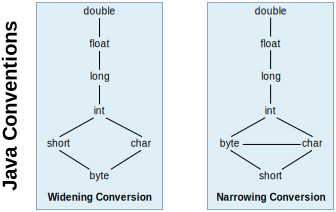
\includegraphics[width=.7\linewidth]{java_type_conversion}
	\end{center}
\end{frame}

\begin{frame}{Implicit and Explicit Type Conversions}
	\begin{description}
	\item[Implicit conversion] conversions automatically done by the compiler, with a possible warning message in the case of narrowing conversion.
		\begin{itemize}
		\item Implicit conversion is also called \emph{coercion}.
		\item Many languages limit the implicit conversions to \emph{widening conversions}.
		\end{itemize}
	\vfill
	\item[Explicit conversion] conversions written in the source code by the programmer.
		\begin{itemize}
		\item Explicit conversion is also called \emph{cast}.
		\end{itemize}
	\end{description}
\end{frame}

\begin{frame}{Function \code{maxType(t$_1$, t$_2$)}}
	\begin{definition}
		$\begin{array}{r@{}l}
			maxType : \mathbb{T} \times \mathbb{T} \rightarrow & \mathbb{T} \\
			(t_1, t_2) \mapsto & \text{maximum or least upper bounds of }t_1\text{ and }t_2 \\
			& \text{in the widening hierarchy. Otherwise error.} \\
		\end{array}$
	\end{definition}
	\begin{example}
		\code{maxType(\kw{short}, \kw{char})} $\rightarrow$ \kw{int}
		\hspace{2em}
		\raisebox{-.9\height}{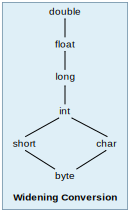
\includegraphics[width=.2\linewidth]{widening_type_conversion}}
	\end{example}
\end{frame}

\begin{frame}{Function \code{widenVar(a, t$_{out}$, t$_{in}$)}}
	\begin{definition}
		$\begin{array}{r@{}l}
			widenVar : \mathbb{A} \times \mathbb{T} \times \mathbb{T} \rightarrow & \mathbb{A} \\
			(a, t_{out}, t_{in}) \mapsto & \text{generates the code that widens the} \\
			& \text{value pointed by }a\text{ to the type }t_{out}\text{,} \\
			& \text{assuming that }a\text{ is of type }t_{in}\text{. This} \\
			& \text{conversion is done only if it is required.} \\
			& \text{Returns the address were the result} \\
			& \text{of the is available.} \\
		\end{array}$
	\end{definition}
\end{frame}

\begin{frame}{Example of Function \code{widenVar(a, t$_{out}$, t$_{in}$)}}
	Assume a language with only the two types \kw{int} and \kw{float}. \\
	\vspace{1em}
	\begin{myfunction}{widenVar}{a : $\mathbb{A}$, t$_{out}$ : $\mathbb{T}$, t$_{in}$ : $\mathbb{T}$}{$\mathbb{A}$}
		\Begin{
			\uIf{t$_{out}$ = t$_{in}$}{
				\Return a;
			}
			\uElseIf{t$_{in}$ = \kw{int} and t$_{out}$ = \kw{float}}{
				t \affect \kw{new} TemporaryVariable()\;
				quadruple(\str{'(float)'}, a, $\emptyset$, t)\;
				\Return t\;
			}
			\Else{
				\throw~\str{"Cannot widen the variable"}\;
			}
		}
	\end{myfunction}
\end{frame}

\begin{frame}{Function \code{narrowVar(a, t$_{out}$, t$_{in}$)}}
	\begin{definition}
		$\begin{array}{r@{}l}
			narrowVar : \mathbb{A} \times \mathbb{T} \times \mathbb{T} \rightarrow & \mathbb{A} \\
			(a, t_{out}, t_{in}) \mapsto & \text{generates the code that narrows the} \\
			& \text{value pointed by }a\text{ to the type }t_{out}\text{,} \\
			& \text{assuming that }a\text{ is of type }t_{in}\text{. This} \\
			& \text{conversion is done only if it is required.} \\
			& \text{Returns the address were the result} \\
			& \text{of the is available.} \\
		\end{array}$
	\end{definition}
\end{frame}

\begin{frame}{Example of Function \code{narrowVar(a, t$_{out}$, t$_{in}$)}}
	Assume a language with only the two types \kw{int} and \kw{float}. \\
	\vspace{1em}
	\begin{myfunction}{narrowVar}{a : $\mathbb{A}$, t$_{out}$ : $\mathbb{T}$, t$_{in}$ : $\mathbb{T}$}{$\mathbb{A}$}
		\Begin{
			\uIf{t$_{out}$ $\neq$ \kw{int} or t$_{in}$ $\neq$ \kw{float}}{
				\throw~\str{"Cannot narrow the variable"}\;
			}
			\uElseIf{t$_{out}$ = \kw{int} and t$_{in}$ = \kw{float}}{
				t \affect \kw{new} TemporaryVariable()\;
				quadruple(\str{'(float)'}, a, $\emptyset$, t)\;
				\Return t\;
			}
			\Else{
				\Return a\;
			}
		}
	\end{myfunction}
\end{frame}

\begin{frame}{Example of Type Conversions in SDD}
	The attribute "\code{type}" is added to store the type of an expression. \\
	The SDD is updated to check the types: \\
	\vspace{1em}
	\begin{sdd}
	\p{E ::= E \tok+ E}{	head.type = \alert{maxType}(E$_1$.type, E$_2$.type) \newl
				o1 = \alert{widenVar}(E$_1$.addr, E$_1$.type, head.type) \newl
				o2 = \alert{widenVar}(E$_2$.addr, E$_2$.type, head.type) \newl
				head.addr = \kw{new} TemporaryVariable() \newl
				quadruple( \str{'+'}, o1, o2, head.addr)}
	\p{E ::= \tok{id} \tok= E}{	head.addr = SymbolTable.getCurrent().get(\tok{id}.lexeme) \newl
					head.type = v.type \newl
					w = \alert{narrowVar}(E.addr, E.type, head.type) \newl
					\kw{if} (w $\neq$ E.addr) \newl
					\hspace{2em}\kw{warning}~\str{"May loose information"} \newl
					\kw{else} \newl
					\hspace{2em}w = \alert{widenVar}(E.addr, E.type, head.type) \newl
					quadruple(\str{'='}, w, $\emptyset$, head.addr)}
	\end{sdd}
\end{frame}

\subsubsection{Overloaded and polymorphic functions}

\tableofcontentslide[sections={3-6},sectionstyle={show/shaded},subsectionstyle={show/shaded/hide},subsubsectionstyle={show/shaded/hide/hide}]

\begin{frame}{Overloading of a Function}
	\begin{definition}
		Allows creating several functions with the same name, which differ from each other in the type of the input and the output of the function.
	\end{definition}
	\begin{itemize}
	\item Depending on the context, the overloading may be for a function, a procedure, a method, or an operator.
	\item \emph{The symbol table must contains all the signatures of the functions (in the context, which is using the symbol table).}
	\item A signature consists of:
		\begin{enumerate}
		\item the function name,
		\item the list of the types of the arguments of the function.
		\end{enumerate}
	\end{itemize}
\end{frame}

\begin{frame}{Polymorphic Function}
	\begin{definition}
			The term ``polymorphic'' refers to any code fragment that can be executed with arguments of different types.
	\end{definition}
	\vspace{2em}
	\begin{itemize}
	\item In this section, we consider the \emph{parametric polymorphism}, where the polymorphism is characterized by parameters or type variables.
	\end{itemize}
\end{frame}

\begin{frame}[fragile]{Example of Polymorphic Function}
	\begin{itemize}
	\item Consider the following definition in ML language:
		\begin{lstlisting}[language=ml]
		fun length(x) = if null(x) then 0 else length( tl(x) ) + 1;
		\end{lstlisting}
	\vfill
	\item Consider the following statement in ML language:
		\begin{lstlisting}[language=ml]
		length( ["sun", "mon", "tue"] ) + length( [10, 9, 8, 7] )
		\end{lstlisting}
	\vfill
	\item The same function \code{length()} is invoked on an array of strings and on an array of integers.
	\vfill
	\item The result of the ML statement is: \code{3 + 4 = 7}
	\end{itemize}
\end{frame}

\begin{frame}{Type of a Polymorphic Function}
	\begin{itemize}
	\item Using the symbol $\forall$ and the type constructor \kw{list}, the type of the function length can be written as:
		\begin{center}
			$\forall a.\kw{list}(a) \rightarrow \kw{int}$
		\end{center}
	\vfill
	\item The $\forall$ symbol is the universal quantifier, and the type variable to which it is applied is said to be bound by it.
	\item A type expression with a $\forall$ symbol in it will be referred as a ``polymorphic type.''
	\vfill
	\item Each time a polymorphic function is applied, its bound type variables (a\dots) can denote a different type.
	\end{itemize}
\end{frame}

\begin{frame}{Determining the Type of a Polymorphic Function}
	\alertbox{How to determine the types in the signature of a polymorphic function?}
	\vspace{1em}
	\alertbox*{We must infer the types by exploring the syntax tree of the function and applying the substitution and unification operations.}
	\begin{description}
	\item[Substitution] A mapping from type variables to type expressions. \inlineexample{\kw{list}(\kw{int}) is an instance of \kw{list}($\alpha$), since it is the result of substituting \kw{int} for $\alpha$ in \kw{list}($\alpha$).}
	\item[Unification] Determine whether type variables $s$ and $t$ are structurally equivalent by substituing the type variables in $s$ and $t$ by type expressions.
	\end{description}
\end{frame}

\begin{frame}[t,fragile]{Example of Type Inference on Polymorphic Function}
	\begin{columns}
		\begin{column}{.4\linewidth}
			\begin{small}
			\begin{lstlisting}[language=ml]
			fun length(x) =
			    if null(x) then 0
			    else length( tl(x) ) + 1;
			\end{lstlisting}
			\end{small}
		\end{column}
		\begin{column}{.6\linewidth}
			\begin{scriptsize}
			\begin{tabularx}{\linewidth}{|X|X|X|}
				\hline
				\tabularheading\chead{Expression}&\chead{Type}&\chead{Unification} \\
				\hline
				\only<1>{	& & \\ \hline}
				\only<2->{	length & $\beta \rightarrow \gamma$ & \\ \hline
						x & $\beta$ & \\ \hline}
				\only<3->{	\kw{if} & $\mathbb{B} \times \alpha \times \alpha \rightarrow \alpha$ & $\alpha = \gamma$\\ \hline}
				\only<4->{	null & $\kw{list}(\omega_n)\rightarrow\mathbb{B}$ & \\ \hline}
				\only<5->{	null(x) & $\mathbb{B}$ & $\kw{list}(\omega_n) = \beta$ \\ \hline}
				\only<6->{	0 & \kw{int} & $\alpha = \kw{int}$ \\ \hline}
				\only<7->{	\kw{+} & $\phi\times\phi\rightarrow\phi$ & $\phi = \alpha$ \\ \hline}
			\end{tabularx}
			\end{scriptsize}
		\end{column}
	\end{columns}
	\putat(-20,-200){\includeanimatedfigure[width=.4\paperwidth]{unification_example}}
	\only<8>{\putat(130,-125){\parbox{20em}{\mdseries\normalcolor\normalsize
		The type of the function "\code{length}" is: \\
		\code{length} : \kw{list}($\omega_n$) $\rightarrow$ \kw{int}
	}}}
\end{frame}

\section[Generation of statements]{Code generation of statements}

\tableofcontentslide[sections={3-},sectionstyle={show/shaded},subsectionstyle={show/show/hide},subsubsectionstyle={hide/hide/hide/hide}]

\subsection{Control flow}

\subsubsection{Introduction}

\tableofcontentslide[sections={3-},sectionstyle={show/shaded},subsectionstyle={show/shaded/hide},subsubsectionstyle={show/show/hide/hide}]

\begin{frame}{Control Flow}
	\begin{itemize}
	\item The translation of statements such as if-else-statements and while-statements is tied to the translation of boolean expressions.
	\item In programming languages, boolean expressions are often used to:
		\begin{enumerate}
		\item Alter the flow of control.
		\item Compute logical values.
		\end{enumerate}
	\item The intended use of boolean expressions is determined by its syntactic context.
	\item To support this distinction, we may:
		\begin{enumerate}
		\item Use two different nonterminals,
		\item Use inherited attributes,
		\item Use a set of flags during the parsing, or
		\item Build a syntax tree and invoke different procedures for the two different uses.
		\end{enumerate}
	\end{itemize}
\end{frame}

\begin{frame}[fragile]{Short-Circuit Code}
	\begin{itemize}
	\item In short-circuit code, the boolean operators translate into \emph{jumps}.
	\item The operators themselves do not appear in the code.
	\item Instead, the value of a boolean expression is represented by a position in the code sequence.
	\end{itemize}
	\begin{example}
		\begin{lstlisting}[linewidth=.6\linewidth,language=Java]
		if ( x < 100 || x > 200 && x != y ) x = 0;
		\end{lstlisting}
		\begin{tac}[.6\linewidth]
		\ifgoto{$x < 100$}{L1}
		\ifnotgoto{$x > 200$}{L2}
		\ifnotgoto{$x \neq y$}{L2}
		\a[L1]{$x$}{$0$}
		\tacdots[L2]
		\end{tac}
	\end{example}
\end{frame}

\subsubsection{Translate the control flow statements}

\tableofcontentslide[sections={3-},sectionstyle={show/shaded},subsectionstyle={show/shaded/hide},subsubsectionstyle={show/shaded/hide/hide}]

\begin{frame}{Statements for Control Flow}
	\begin{itemize}
	\item Consider the grammar:
		\raisebox{-.5\height}{
		\begin{footnotesize}
		\begin{bnf}[.5\linewidth]
		\p{S ::= \tok{if} \tok( B \tok) S}
		\p{  ::= \tok{if} \tok( B \tok) S \tok{else} S}
		\p{  ::= \tok{while} \tok( B \tok) S}
		\end{bnf}
		\end{footnotesize}}
	\vfill
	\item We introduce the attributes:
		\begin{itemize}
		\item \tactext{B.code} and \tactext{S.code}: synthesized attributes; three-address code of the nonterminals.
		\item \tactext{B.true}: inherited attribute; the label of the code associated to the then-statements.
		\item \tactext{B.false}: inherited attribute; the label of the code associated to the else-statements.
		\item \tactext{B.next}: inherited attribute; the label of the code just after the current if-then-else statements.
		\end{itemize}
	\end{itemize}
\end{frame}

\begin{frame}{Statement \kw{if}-\kw{then}}
	\begin{columns}
		\begin{column}{.4\linewidth}
			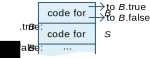
\includegraphics[width=\linewidth]{statement_if}
		\end{column}
		\begin{column}{.6\linewidth}
			\begin{footnotesize}
			\begin{sdd}
			\p{S ::= \tok{if} \tok(}{	B.true = newlabel() \newl
							B.false = head.next}
			\pcont{B \tok)}{		S.next = head.next \newl
							label(B.true)}
			\pcont{S}{}
			\end{sdd}
			\end{footnotesize}
		\end{column}
	\end{columns}
	\begin{itemize}
	\vfill
	\item The nontemirnal for the condition is no more $E$, but $B$.
	\item The function \tactext{newlabel()} creates a new label each time it is called.
	\item The function \tactext{label(L)} attaches label \tactext{L} to the next three-address instruction to be generated.
	\end{itemize}
\end{frame}

\begin{frame}{Statement \kw{if}-\kw{then}-\kw{else}}
	\begin{columns}
		\begin{column}{.4\linewidth}
			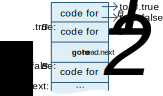
\includegraphics[width=\linewidth]{statement_if_else}
		\end{column}
		\begin{column}{.6\linewidth}
			\begin{footnotesize}
			\begin{sdd}
			\p{S ::= \tok{if} \tok(}{	B.true = newlabel() \newl
							B.false = newlabel()}
			\pcont{B \tok)}{		S$_1$.next = head.next \newl
							label(B.true)}
			\pcont{S \tok{else}}{		quadruple(\str{'goto'}, \newl
							\hspace{1em}head.next, \newl
							\hspace{1em}$\emptyset$, $\emptyset$) \newl
							S$_2$.next = head.next \newl
							label(B.false)}
			\pcont{S}{}
			\end{sdd}
			\end{footnotesize}
		\end{column}
	\end{columns}
\end{frame}

\begin{frame}{Statement \kw{while}}
	\begin{columns}
		\begin{column}{.4\linewidth}
			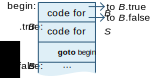
\includegraphics[width=\linewidth]{statement_while}
		\end{column}
		\begin{column}{.6\linewidth}
			\begin{footnotesize}
			\begin{sdd}
			\p{S ::= \tok{while} \tok(}{	begin = newlabel() \newl
							B.true = newlabel() \newl
							B.false = head.next}
			\pcont{B \tok)}{		S.next = begin \newl
							label(B.true)}
			\pcont{S}{			quadruple(\str{'goto'}, \newl
							\hspace{1em}begin, \newl
							\hspace{1em}$\emptyset$, $\emptyset$)}
			\end{sdd}
			\end{footnotesize}
		\end{column}
	\end{columns}
\end{frame}

\subsubsection{Boolean expressions for Control Flow}

\tableofcontentslide[sections={3-},sectionstyle={show/shaded},subsectionstyle={show/shaded/hide},subsubsectionstyle={show/shaded/hide/hide}]

\begin{frame}{Boolean Constants in the Control Flow}
	\begin{itemize}
	\item Boolean expressions dedicated to control flow need dedicated semantic rules.
	\item Remember that the boolean expressions used in control-flow statements must be translated into jumping three-address code.
	\end{itemize}
	\begin{sdd}
	\p{B ::= \tok{true}}{quadruple(\str{'goto'}, head.true, $\emptyset$, $\emptyset$)}
	\p{B ::= \tok{false}}{quadruple(\str{'goto'}, head.false, $\emptyset$, $\emptyset$)}
	\end{sdd}
\end{frame}

\begin{frame}{Boolean Operator NOT}
	\begin{columns}
		\begin{column}{.4\linewidth}
			\begin{center}
			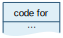
\includegraphics[width=.5\linewidth]{statement_not}
			\end{center}
		\end{column}
		\begin{column}{.6\linewidth}
			\begin{footnotesize}
			\begin{sdd}
			\p{B ::= \tok{\string!} B}{	B.true = head.false \newl
							B.false = head.true}
			\end{sdd}
			\end{footnotesize}
		\end{column}
	\end{columns}
	\vfill
	\begin{itemize}
	\item No code is needed for an expression of the form \tactext{\tok{\string!}B}.
	\item Just interchange the \tactext{true} and \tactext{false} attributes of the head to set the \tactext{true} and \tactext{false} attributes of $B$.
	\end{itemize}
\end{frame}

\begin{frame}{Boolean Operator OR}
	\begin{columns}
		\begin{column}{.45\linewidth}
			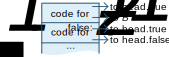
\includegraphics[width=\linewidth]{statement_or}
		\end{column}
		\begin{column}{.55\linewidth}
			\begin{footnotesize}
			\begin{sdd}
			\p{B ::=}{	B$_1$.true = head.true \newl
					B$_1$.false = newlabel()}
			\pcont{B}{	B$_2$.true = head.true \newl
					B$_2$.false = head.false}
			\pcont{\tok{\textbar\textbar} B}{}
			\end{sdd}
			\end{footnotesize}
		\end{column}
	\end{columns}
	\vfill
	\begin{itemize}
	\item If \bnftext{B$_1$} is true, the head is true.
	\item If \bnftext{B$_1$} is false, evaluate \bnftext{B$_2$}.
	\item So \bnftext{B$_1$.false} is the label of the first instruction of \bnftext{B$_2$}.
	\item The value of the head becomes the same as the value of \bnftext{B$_2$}.
	\end{itemize}
\end{frame}

\begin{frame}{Boolean Operator AND}
	\begin{columns}
		\begin{column}{.45\linewidth}
			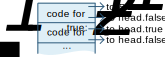
\includegraphics[width=\linewidth]{statement_and}
		\end{column}
		\begin{column}{.55\linewidth}
			\begin{footnotesize}
			\begin{sdd}
			\p{B ::=}{	B$_1$.true = newlabel() \newl
					B$_1$.false = head.false}
			\pcont{B}{	B$_2$.true = head.true \newl
					B$_2$.false = head.false}
			\pcont{\tok{\&\&} B}{}
			\end{sdd}
			\end{footnotesize}
		\end{column}
	\end{columns}
	\vfill
	\begin{itemize}
	\item If \bnftext{B$_1$} is false, the head is false.
	\item If \bnftext{B$_1$} is true, evaluate \bnftext{B$_2$}.
	\item So \bnftext{B$_1$.true} is the label of the first instruction of \bnftext{B$_2$}.
	\item The value of the head becomes the same as the value of \bnftext{B$_2$}.
	\end{itemize}
\end{frame}

\begin{frame}{Operators of Comparison}
	\begin{columns}
		\begin{column}{.3\linewidth}
			\begin{center}
			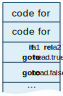
\includegraphics[width=.7\linewidth]{statement_rel}
			\end{center}
		\end{column}
		\begin{column}{.7\linewidth}
			\begin{footnotesize}
			\begin{sdd}
			\p{B ::= E \tok{rel} E}{	t = \kw{new} TemporaryVariable() \newl
							quadruple(\tok{rel}.operator, \newl
							\hspace{1em}E$_1$.addr, E$_2$.addr, t) \newl
							quadruple(\str{'if'}, t, \newl
							\hspace{1em}head.true, $\emptyset$) \newl
							quadruple(\str{'goto'}, head.false, \newl
							\hspace{1em}$\emptyset$, $\emptyset$)}
			\end{sdd}
			\end{footnotesize}
		\end{column}
	\end{columns}
	\vfill
	\begin{itemize}
	\item The form $a<b$ translates into: \\
		\tactext{t = ($a<b$)} \\
		\tactext{\kw{if} t \tok{then} \kw{goto} B.true} \\
		\tactext{\kw{goto} B.false} \\
	\end{itemize}
\end{frame}

\begin{frame}[fragile]{Example of Translation}
	\begin{lstlisting}[language=Java]
		if ( x < 100 || x > 200 && x != y ) x = 0;
	\end{lstlisting}
	\vfill
	\begin{tac}
	\a{\t1}{$x < 100$}
	\ifgoto{\t1}{L2}
	\goto{L3}
	\a[L3]{\t1}{$x > 200$}
	\ifgoto{$x > 200$}{L4}
	\goto{L1}
	\a[L4]{\t1}{$x \neq y$}
	\ifgoto{\t1}{L2}
	\goto{L1}
	\a[L2]{x}{0}
	\tacdots[L1]
	\end{tac}
\end{frame}

\subsubsection{Avoid redundant goto}

\tableofcontentslide[sections={3-},sectionstyle={show/shaded},subsectionstyle={show/shaded/hide},subsubsectionstyle={show/shaded/hide/hide}]

\begin{frame}{Redundant Goto Statements}
	\begin{small}
	\alertbox{The semantic rules described in the previous slides may generate more goto instructions than strictly necessary.}
	\begin{example}
		\begin{tac}
		\a[L3]{\t1}{$x>200$}
		\ifgoto{\t1}{L4}
		\goto{L1}
		\tacdots[L4]
		\tacdots[L1]
		\end{tac}
	\end{example}
	\begin{block}{Best Practice}
		\begin{tac}
		\a[L3]{\t1}{$x>200$}
		\ifnotgoto{\t1}{L1}
		\tacdots
		\tacdots[L1]
		\end{tac}
	\end{block}
	\end{small}
\end{frame}

\begin{frame}{Remove Redundant Gotos}
	\begin{itemize}
	\item Avoiding redundant gotos is done by introducing a constant for the value of the labels: \tactext{fall}.
	\item This constant means ``don't generate any jump.'', or ``fall in the next available instruction.''
	\vfill
	\item We can adapt the semantic rules of the boolean expressions. \bnftext{S \bnfbody \tok{if} \tok( B \tok) S}.
	\end{itemize}
	\begin{tabularx}{\linewidth}{@{}XcX@{}}
		\begin{scriptsize}
		\begin{sdd}
		\p{S ::= \tok{if} \tok(}{	B.true = newlabel() \newl
						B.false = head.next}
		\pcont{B \tok)}{		S.next = head.next \newl
						label(B.true)}
		\pcont{S}{}
		\end{sdd}
		\end{scriptsize}
		& \pgfuseimage{rightarrow}
		&
		\begin{scriptsize}
		\begin{sdd}
		\p{S ::= \tok{if} \tok(}{	B.true = \tok{fall} \newl
						B.false = head.next}
		\pcont{B \tok)}{		S.next = head.next}
		\pcont{S}{}
		\end{sdd}
		\end{scriptsize}
	\end{tabularx}
\end{frame}

\pgfdeclareimage[height=2em]{bottomarrow}{imgs/all/bottomarrow}

\begin{frame}{Remove Redundant Gotos of the OR Operator}
	\begin{center}
		\begin{footnotesize}
		\begin{sdd}[.7\linewidth]
		\p{B ::=}{	B$_1$.true = head.true \newl
				B$_1$.false = newlabel()}
		\pcont{B}{	B$_2$.true = head.true \newl
				B$_2$.false = head.false}
		\pcont{\tok{\textbar\textbar} B}{}
		\end{sdd}
		\end{footnotesize} \\[1em]
		\pgfuseimage{bottomarrow} \\[1em]
		\begin{footnotesize}
		\begin{sdd}[.7\linewidth]
		\p{B ::=}{	\kw{if} head.true = \kw{fall} \newl
				\hspace{1em}B$_1$.true = newlabel() \newl
				\kw{else} \newl
				\hspace{1em}B$_1$.true = head.true \newl
				B$_1$.false = \kw{fall}}
		\pcont{B}{	B$_2$.true = head.true \newl
				B$_2$.false = head.false}
		\pcont{\tok{\textbar\textbar} B}{
				\kw{if} head.true = \kw{fall} \newl
				\hspace{1em}label(B$_1$.true)}
		\end{sdd}
		\end{footnotesize}
	\end{center}
\end{frame}

\subsection{Backpatching}

\subsubsection{Introduction}

\tableofcontentslide[sections={3-},sectionstyle={show/shaded},subsectionstyle={show/shaded/hide},subsubsectionstyle={show/show/hide/hide}]

\begin{frame}[allowframebreaks]{Problem with Jumps}
	\alertbox{A key problem is the matching of a jump instruction with the target address of the jump.}
	\vspace{1em}
	\begin{example}
		\begin{itemize}
		\item Consider the statement \bnftext{\tok{if} \tok( B \tok) S}.
		\item In a \emph{one-pass translation}, $B$ must be translated before $S$ is examined.
		\item \emph{What is the address of the label that permits to go over the code for $S$?}
		\end{itemize}
	\end{example}
	%
	\framebreak
	%
	\begin{block}{Solution 1}
		\begin{itemize}
		\item In the previous slides, we solve this problem by using inherited attributes "\texttt{next}".
		\item \alert{But a separate pass is then needed to bind labels to addresses.}
		\end{itemize}
	\end{block}
	\vspace{1em}
	\begin{block}{Solution 2}
		\begin{itemize}
		\item \emph{Backpatching} can be used to generate code for boolean expressions and flow-of-control statements in one pass.
		\item This approach is detailled in the following slides.
		\end{itemize}
	\end{block}
\end{frame}

\begin{frame}{General Principle of Backpatching}
	\begin{itemize}
	\item When the jump target is after the current instruction, the address of the current instruction is added into a list.
	\vspace{2em}
	\item When the address of the target instruction is known, the instructions in the list are updated.
	\end{itemize}
\end{frame}

\begin{frame}{New attributes for the Backpatching}
	\begin{itemize}
	\item Introduction of synthesized attributes: \emph{bptruelist} and \emph{bpfalselist} of the nonterminal $B$ are used to manage labels in jumping code for \emph{boolean expressions}.
	\vfill
		\begin{description}
		\item[B.bptruelist] list of jump or conditional jump instructions into which we must insert the label to which control goes if $B$ is true.
	\vfill
		\item[B.bpfalselist] list of instructions that eventually get the label to which control goes when $B$ is false.
		\end{description}
	\vfill
	\item Similarly, the other productions, such as $S$, must be updated in a simular way with synthesized attributes.
	\end{itemize}
\end{frame}

\begin{frame}{Tools for the Backpatching}
	\begin{description}
	\item[makebplist(adr)] creates a new list containing only $adr$, an index into the array of instructions.
	\vfill
	\item[mergebplists(lst1,lst2)] concatenates the lists pointed by $lst1$ and $lst2$, and returns a pointer to the result.
	\vfill
	\item[backpatch(lst,adr)] inserts $adr$ as the target label for each of the instructions on the list pointed to by $lst$.
	\vfill
	\item[instadr()] replies the address of the instruction that will be generated by the \Emph{next} call to \tactext{quadruple()}.
	\vfill
	\item[Unknown address] The keyword \kw{?} represents an unkwown address.
	\end{description}
\end{frame}

\begin{frame}{Backpatching of the Boolean Control-Flow Rules}
	\begin{sdd}
	\p{B ::= \tok{true}}{	\emph{head.bptruelist = makebplist(instadr())} \newl
				quadruple(\str{'goto'}, \emph{\kw{?}}, $\emptyset$, $\emptyset$)}
	\hline
	\p{B ::= \tok{false}}{	\emph{head.bpfalselist = makebplist(instadr())} \newl
				quadruple(\str{'goto'}, \emph{\kw{?}}, $\emptyset$, $\emptyset$)}
	\hline
	\p{B ::= E \tok{rel} E}{	t = \kw{new} TemporaryVariable() \newl
					quadruple(\tok{rel}.operator, E$_1$.addr, E$_2$.addr, t) \newl
					\emph{head.bptruelist = makebplist(instadr())} \newl
					quadruple(\str{'if'}, t, \emph{\tok{?}}, $\emptyset$) \newl
					\emph{head.bpfalselist = makebplist(instadr())} \newl
					quadruple(\str{'goto'}, \emph{\tok{?}}, $\emptyset$, $\emptyset$)}
	\hline
	\p{B ::= B \tok{\textbar\textbar}}{	\emph{backpatch(B$_1$.bpfalselist, instadr())}}
	\pcont{B}{				\emph{head.bptruelist = mergbplists(} \newl
						\hspace{1em}\emph{B$_1$.bptruelist, B$_2$.bptruelist)} \newl
						\emph{head.bpfalselist = B$_2$.bpfalselist}}
	\end{sdd}
\end{frame}

\begin{frame}{Backpatching of the Control-Flow Statements}
	\begin{small}
	\begin{sdd}
	\p{S ::= \tok{if} \tok( B \tok)}{	backpatch(B.bptruelist, instadr())}
	\pcont{S}{				head.\emph{bpnextlist} = mergebplists(B.bpfalselist, S.\emph{bpnextlist})}
	\hline
	\p{S ::= \tok{if} \tok( B \tok)}{	backpatch(B.bptruelist, instadr())}
	\pcont{S \tok{else}}{			backpatch(B.bpfalselist, instadr())}
	\pcont{S}{				head.\emph{bpnextlist} = mergebplists(S$_1$.\emph{bpnextlist}, S$_2$.\emph{bpnextlist})}
	\hline
	\p{S ::= \tok{while}}{		a = instadr()}
	\pcont{\tok( B \tok)}{		backpatch(B.bptruelist, instadr())}
	\pcont{S}{			backpatch(S.\emph{bpnextlist}, a) \newl
					quadruple(\str{'goto'}, a, $\emptyset$, $\emptyset$) \newl
					head.\emph{bpnextlist} = B.bpfalselist}
	\end{sdd}
	\vfill
	The attribute \tactext{bpnextlist} is the list of the addresses of the instructions that are refering the ``next instruction.''
	\end{small}
\end{frame}

\begin{frame}{Algorithm of \code{backpatch()}}
	\begin{scriptsize}
	\begin{myprocedure}{backpatch}{list, address}
	\Input{$\mathbb{Q}$ is the global list of the generated quadruples.}
	\Begin{
		\ForEach{$a \in list$}{
			q \affect $\mathbb{Q}[a]$\;
			\uIf{q.op = \str{'goto'}}{
				\lIf{q.arg$_1$ $\neq$ \kw{?}}{\throw~\str{"Cannot backpatch"}}\;
				q.arg$_1$ \affect address\;
			}
			\uElseIf{q.op = \str{'if'}}{
				\lIf{q.arg$_2$ $\neq$ \kw{?}}{\throw~\str{"Cannot backpatch"}}\;
				q.arg$_2$ \affect address\;
			}
			\uElseIf{q.op = \str{'ifFalse'}}{
				\lIf{q.arg$_2$ $\neq$ \kw{?}}{\throw~\str{"Cannot backpatch"}}\;
				q.arg$_2$ \affect address\;
			}
			\Else{
				\throw~\str{"Instruction to backpatch not found"}\;
			}
		}
	}
	\end{myprocedure}
	\end{scriptsize}
\end{frame}

\section{Conclusion}

\tableofcontentslide[sectionstyle={show/shaded},subsectionstyle={hide/hide/hide},subsubsectionstyle={hide/hide/hide/hide}]

\begin{frame}[t,allowframebreaks]{Key Concepts in the Chapter}
	\begin{description}
	\item[Inherited and synthesized attributes] Syntax-directed definitions may use two kinds of attributes. A synthesized attribute at a parse-tree node is computed from attributes at its children. An inherited attribute at a node is computed from attributes at its parent and/or siblings.
	\item[Dependency graphs] Given a parse tree and an SDD, we draw edges among the attribute instances associated with each parse-tree node to denote that the value of the attribute at the head of the edge is computed in terms of the value of the attribute at the tail of the edge.
	\item[S-Attributed definitions] In a S-attributed SDD, all attributes are synthesized.
	\item[L-Attributed definitions] In a L-attributed SDD, attributes may be inherited or synthesized. However, inherited attributes at a parse-tree node may depend only on inherited attributes of its parent and on (any) attributes of siblings to its left.
Syntax trees: Each node in a syntax tree represents a construct; the children of the node represent the meaningful components of the construct.
	\item[Intermediate representation] An intermediate representation is typically some combination of a graphical notation and three-address code. As in syntax, a node in a graphical notation represents a construct; the children of a node represent its subconstructs. Three address code takes its name from instructions of the form \tactext{x = y \kw{op} z}, with at most one operator per instruction. There are additional instructions for control flow.
	\item[Translate expressions] Expressions with built-up operations can be unwound into a sequence of individual operations by attaching actions to each production of the form \bnftext{E \bnfbody E$_1$ \tok{op} E$_2$}. The action either creates a node for \bnftext{E} with the nodes for \bnftext{E$_1$} and \bnftext{E$_2$} as children, or it generates a three-address instruction that applies op to the addresses for \bnftext{E$_1$} and \bnftext{E$_2$} and puts the result into a new temporary name, which becomes the address of \bnftext{E}.
	\item[Check types] The type of an expression \tactext{E$_1$ \kw{op} E$_1$} is determined by the operator \kw{op} and the types of \tactext{E$_1$} and \tactext{E$_2$}. A coercion is an implicit type conversion. Intermediate code contains explicit type conversions to ensure an exact match between operand types and the types expected by an operator.
	\item[Generate jumping code for boolean expression] In short-circuit or jumping code, the value of a boolean expression is implicit in the position reached in the code. Jumping code is useful because a boolean expression $B$ is typically used to \tactext{t=true} or \tactext{t=false}, as appropriate, where \tactext{t} is a temporary name. Using labels for jumps, a boolean expression can be translated by inheriting labels corresponding to its true and false exits attributes. The constants \kw{true} and \kw{false} translate into a jump to the true and false attributes, respectively.
	\item[Implement statements using control flow] Statements can be translated by inheriting a label next, where next marks the first instruction after the code for this statement. The conditional \bnftext{S \bnfbody \tok{if} \tok( B \tok) S} can be translated by attaching a new label marking the beginning of the code for \bnftext{S} and passing the new label and \tactext{S.next} for the true and false attributes, respectively, of $B$.
	\item[Alternatively, use backpatching] Backpatching is a technique for generating code for boolean expressions and statements in one pass. The idea is to maintain lists of incomplete jumps, where all the jump instructions on a list have the same target. When the target becomes known, all the instructions on its list are completed by filling in the target.
	\item[Implement records] Field names in a record or class can be treated as a sequence of declarations. A record type encodes the types and relative addresses of the fields. A symbol table object can be used for this purpose.
	\end{description}
\end{frame}

\begin{frame}[t,allowframebreaks]{\bibname\ of the Chapter}%
	\tiny%
	\putbib[bibliographies/chapter4]%
\end{frame}%

\end{bibunit}

% Reset the style of the navigation box
\setbeamertemplate{headline text style}{}



%\begin{bibunit}[apalike]

\part[author={Stéphane GALLAND},label={chap:runtime_environments}]{Run-time Environments}

\tableofcontentslide

\section{Introduction}

\begin{frame}{Introduction}
	\begin{itemize}
	\item A compiler must implement the abstractions embodied in the source-language definition.
	\vfill
	\item \emph{The compiler must cooperate with the operating system and other systems software to support these abstracts on the target machine.}
	\vfill
	\item To do so, the compiler creates and manages a \Emph{run-time environment} in which it assumes its target programs are being executed.
	\vfill
	\item \alert{This chapter presents the key points of the run-time environment:}
		\begin{enumerate}
		\item Management of the Heap,
		\item Management of the Stack,
		\item Dynamic Memory Deallocation.
		\end{enumerate}
	\end{itemize}
\end{frame}

\section{Data Storage}

\tableofcontentslide[sectionstyle={show/shaded},subsectionstyle={show/show/hide},subsubsectionstyle={hide/hide/hide/hide}]

\begin{frame}{Storage Organization}
	\begin{itemize}
	\item The target program runs in its own \emph{logical address space} in which each value has a location.
	\item The organization and management of this logical address space is shared between: \begin{itemize}
		\item the compiler,
		\item the operating system,
		\item the target machine.
		\end{itemize}
	\vfill
	\item The operating system maps the logical addresses into physical addresses.
	\item When defined, a \emph{virtual machine} is a program that is representing the operating system and the target machine into an abstract and platform-independent machine.
	\end{itemize}
\end{frame}

\sidecite{Randell.1964}
\begin{frame}[t]{Structure of the Logicial Address Space}
	\begin{itemize}
	\item In the run-time environment, the logical address space has a structure; typically:
	\end{itemize}
	\vfill
	\begin{columns}
		\begin{column}{.3\linewidth}
			\raisebox{-.5\height}{\includeanimatedfigure[width=\linewidth]{address_space_structure}}
		\end{column}
		\begin{column}{.7\linewidth}\begin{small}
			\only<2>{\begin{itemize}
				\item The compiler can place the executable target code in a statically determined area, named Code.
				\item This area contains the binary representations of the instructions to execute.
				\item The format of the code depends on the target machine: Intel binary assembler, byte code\dots
				\end{itemize}}
			\only<3>{\begin{itemize}
				\item Similarly, the size of some program data may be known at compile time.
				\item The area where these data are stored in named Static area, usually put just after the Code area.
				\item \inlineexamples{string literals, global constants and variables, information related to garbage collection\dots}
				\item The addresses of the static data are directly put in the code.
				\end{itemize}}
			\only<4>{\begin{itemize}
				\item The stack is used to store data structures called activation records.
				\item Activation records are generated during the procedure/function calls (explained later).
				\item Basically, each record contains the status of the machine: ordinal counter, machine registers, and data whose lifetimes are the same as the activation time (usually local variables).
				\end{itemize}}
			\only<5>{\begin{itemize}
				\item Many languages allow the programmer to allocate and deallocate data under program control (malloc, new\dots)
				\item The heap is used to manage this kind of long-lived data.
				\end{itemize}}
			\only<6>{\begin{itemize}
				\item The heap and the stack are growing up and consume the free memory space between them.
				\item When the stack cannot grow up, the classical ``stack overflow'' error is fired.
				\item When the heap cannot grow up, the classical ``out of memory'' error is fired.
				\end{itemize}}
			\end{small}
		\end{column}
	\end{columns}
\end{frame}

\begin{frame}{Static vs. Dynamic Storage Allocation}
	The layout and allocation of data to memory locations in the run-time environment are key issues in storage management.
	\vfill
	\begin{block}{Static Storage Allocation}
		It is made \emph{by the compiler} looking only at the text of the program, not at what the program does when it executes.
	\end{block}
	\vfill
	\begin{block}{Dynamic Storage Allocation}
		\begin{itemize}
		\item It is made only \emph{while the program is running}.
		\item Many compilers use a combination of the strategies explained in the following slide for dynamic storage allocation.
		\end{itemize}
	\end{block}
\end{frame}

\sidecite{Randell.1964}
\begin{frame}{Strategies for Dynamic Storage Allocation}
	\begin{block}{Stack Storage}
		\begin{itemize}
		\item Names local to a procedure are allocated space \emph{on a stack}.
		\item The stack supports the normal call/return policy for procedures.
		\end{itemize}
	\end{block}
	\vfill
	\begin{block}{Heap Storage}
		\begin{description}
		\item Data that may outlive the call to the procedure that created it is usually allocated \emph{on a ``heap''} of reusable storage.
		\item The heap is an area of virtual memory that allows data to obtain and release storage.
		\item[Garbage collection] the run-time environment detects useless data in heap and releases them.
		\end{description}
	\end{block}
\end{frame}

\section{Stack management}

\tableofcontentslide[sectionstyle={show/shaded},subsectionstyle={show/show/hide},subsubsectionstyle={hide/hide/hide/hide}]

\subsection{Stack allocation}

\subsubsection{Introduction}

\tableofcontentslide[sections={1-4},sectionstyle={show/shaded},subsectionstyle={show/shaded/hide},subsubsectionstyle={show/show/hide/hide}]

\sidecite{Randell.1964}
\begin{frame}{Stack Allocation}
	\begin{description}
	\item Compilers that use procedures, functions, or methods as units manage a part of their run-time memory as a stack.
	\item[Note] procedure will be used as a generic term for procedure, function and method.
	\vfill
	\item Each time a procedure is called:
		\begin{itemize}
		\item space for its local variables is pushed into a stack.
		\end{itemize}
	\item When the procedure terminates:
		\begin{itemize}
		\item space is popped off the stack.
		\end{itemize}
	\vfill
	\item The activation of procedure $\equiv$ the call to the procedure.
	\end{description}
\end{frame}

\begin{frame}[fragile]{Nested Activation in Time}
	\begin{small}
	\alertbox{Stack allocation would not be feasible if procedure calls did not nest in time.}
	\begin{columns}
		\begin{column}{.5\linewidth}
			\begin{itemize}
			\item If an activation of procedure \code{p} calls procedure \code{q}, then that activation of \code{q} must end before the activation of \code{p} can end.
			\end{itemize}
			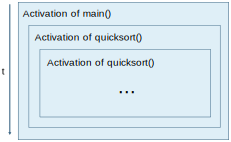
\includegraphics[width=\linewidth]{nested_activation}
		\end{column}
		\begin{column}{.5\linewidth}
			\begin{lstlisting}[language=C,basicstyle=\Tiny]
			int a[11];
			void readArray() {
			    int i; // read and fill a
			}
			int partition(int m, int n) {
			    // let v, a[m..p-1] < v, a[p]=v, a[p+1..n] >= v
			    // return p
			}
			void quicksort(int m, int n) {
			    int i;
			    if (n>m) {
			        i = partition(m,n);
			        quicksort(m,i-1);
			        quicksort(i+1,n);
			    }
			}
			main() {
			    readArray();
			    a[0] = -9999;
			    a[11] = 9999;
			    quicksort(1,9);
			}
			\end{lstlisting}
		\end{column}
	\end{columns}
	\end{small}
\end{frame}

\begin{frame}[allowframebreaks]{Termination of Nested Activation}
	Three common cases when \code{p} calls \code{q}:
	\vspace{1em}
	\begin{enumerate}
	\item[Normal] The activation of \code{q} terminates normally. Then in essentially any language, control resumes just after the point of \code{p} at which the call to \code{q} was made.
	\vspace{1em}
	\item[Abort] The activation of \code{q}, or some procedure called by \code{q}, either directly or indirectly, aborts.
\code{p} ends simultaneously with \code{q}.
	\item[Exception] The activation of \code{q} terminates because of an exception that \code{q} cannot handle. \\
		Procedure \code{p} may handle the exception: the activation of \code{q} has terminated but \code{p} continues (not necessary where \code{q} was called). \\
		If \code{p} cannot handle the exception, then this activation of \code{p} terminates at the same time as the activation of \code{q}, and presumably, the exception will be handled by some other open activation of a procedure.
	\end{enumerate}
\end{frame}

\subsubsection{Activation tree}

\tableofcontentslide[sections={1-4},sectionstyle={show/shaded},subsectionstyle={show/shaded/hide},subsubsectionstyle={show/shaded/hide/hide}]

\begin{frame}{Activation Tree}
	The activations of procedures during the running of an entire program is represented by a tree, named \emph{activation tree}.
	\vfill
	\begin{description}
	\item[Node] an activation;
	\vfill
	\item[Root Node] the root is the activation of the ``main'' procedure that initiates the execution of the program.
	\vfill
	\item[Child Node] activations of the procedures called by the activation represented by the parent node. The order of the children (from left to right) is the order of the activations.
	\end{description}
\end{frame}

\figureslide{Example of Activation Tree}{activation_tree_example}

\subsubsection{Control Stack and Activation record}

\tableofcontentslide[sections={1-4},sectionstyle={show/shaded},subsectionstyle={show/shaded/hide},subsubsectionstyle={show/shaded/hide/hide}]

\begin{frame}{Control Stack and Activation Record}
	\begin{itemize}
	\item Procedure calls and returns are usually managed by a run-time stack called the \emph{control stack}.
	\vfill
	\item Each live activation has an \emph{activation record} (or frame) on the control stack.
	\vfill
	\item The entire sequence of activation records on the stack corresponding to the path in the activation tree to the activation where control currently resides.
	\vfill
	\item \emph{The latter activation has its record at the top of the stack.}
	\end{itemize}
\end{frame}

\figureslide{Example of Control Stack}{control_stack_example}

\begin{frame}[t]{Structure of the Activation Record}
	\begin{itemize}
	\item The contents of activation records vary with the language being implemented; typically:
	\end{itemize}
	\vfill
	\begin{columns}
		\begin{column}{.3\linewidth}
			\raisebox{-.5\height}{\includeanimatedfigure[width=\linewidth]{activation_record_structure}}
		\end{column}
		\begin{column}{.7\linewidth}\begin{small}
			\only<2>{\begin{itemize}
				\item Temporary values, such as those arising from the evaluation of expressions, in cases where the temporaries cannot be held in registers.
				\end{itemize}}
			\only<3>{\begin{itemize}
				\item Local data belonging to the procedure whose activation record this is.
				\end{itemize}}
			\only<4>{\begin{itemize}
				\item Information about the state of the machine just before the call to the procedure.
				\item It typically includes:
					\begin{description}
					\item[return address] the value of the ordinal counter to which the called procedure must return.
					\item[Registers] The contents of registers that were used by the calling procedure and that must be restored when the return occurs.
					\end{description}
				\end{itemize}}
			\only<5>{\begin{itemize}
				\item An ``access link'' may be needed to locate data needed by the called procedure but found elsewhere (in another activation record\dots)
				\end{itemize}}
			\only<6>{\begin{itemize}
				\item A ``control link'' is pointing to the activation record of the caller.
				\end{itemize}}
			\only<7>{\begin{itemize}
				\item Space for the return value of the called function, if any.
				\item Not all called procedures return a value.
				\item We may prefer to place that value in a register for efficiency.
				\end{itemize}}
			\only<8>{\begin{itemize}
				\item The actual parameters are given by the caller and used by the callee procedure.
				\item Commonly, these values are not placed in the activation record but rather in registers, when possible.
				\end{itemize}}
			\end{small}
		\end{column}
	\end{columns}
\end{frame}

\subsubsection{Calling sequence}

\tableofcontentslide[sections={1-4},sectionstyle={show/shaded},subsectionstyle={show/shaded/hide},subsubsectionstyle={show/shaded/hide/hide}]

\sidecite{Johnson.1981}
\begin{frame}{Calling and Return Sequence}
	\begin{definition}[Calling Sequence]
		A calling sequence is a \code{code} that allocates an activation record on the stack and enters information into its fields.
	\end{definition}
	\begin{definition}[Return Sequence]
		A return sequence is a \code{code} that deallocates an activation record from the stack and restores the state of the machine.
	\end{definition}
	\vfill
	\alertbox{Calling sequences and the layout of activation records may differ greatly, even among implementations of the same language.}
	\vfill
	\begin{itemize}
	\item The calling sequence is composed of: \begin{itemize}
		\item Calling procedure (the ``caller''),
		\item Called procedure (the ``callee'').
		\end{itemize}
	\end{itemize}
\end{frame}

\sidecite{Randell.1964}
\begin{frame}[t]{Principles of the Calling Sequences}
	\putat(180,-200){\includeanimatedfigure[width=.4\paperwidth]{calling_sequence_principles}}
	When designing calling sequences and the layout of the activation records, the following principles are used:
	\only<1>{\begin{enumerate}
		\item \emph{Values communicated between caller and callee are generally placed at the beginning of the callee activation record.}
		\end{enumerate}}
	\only<2>{\begin{enumerate}
		\setcounter{enumi}{1}
		\item \emph{Fixed-length items are placed in the middle of the record.}
		\end{enumerate}}
	\only<3>{\begin{enumerate}
		\setcounter{enumi}{2}
		\item \emph{Items whose size may not be known early enough are placed at the end of the activation record.}
		\end{enumerate}}
	\only<4>{\begin{enumerate}
		\setcounter{enumi}{3}
		\item \emph{We must locate the ``top-of-stack'' pointer judiciously.}
		\end{enumerate}}
	\vspace{1em}
	\hspace{2em}\begin{minipage}{.5\linewidth}
		\only<1>{	\small
				\nohyphens{The caller can compute the actual parameters and put them at the top of the stack, without the necessity to create the entire record of the callee, and knowing how the callee's record layout is.}
				\par
				\nohyphens{The caller knows where to put the return value, relative to its own record.}
		}
		\only<2>{	\small
				\nohyphens{If machine status are standardized, then programs such as debuggers will have an easier time deciphering the stack contents if an error occurs.}
		}
		\only<3>{	\small
				\nohyphens{Most of the variables have a size that can be determined by the compiler. But some cannot (dynamic arrays\dots)}
				\par
				\nohyphens{The amount of space needed for temporaries is not known during the first phase of the intermediate code generation.}
		}
		\only<4>{	\small
				\nohyphens{Commonly, it points to the end of the fixed-length fields in the activation record.}
				\par
				\nohyphens{The control link points to the ``top-of-stack'' of the previous record.}
				\par
				\nohyphens{Fixed-length data can then be accessed by fixed negative offset, and variable-length with a run-time positive offset.}
		}
	\end{minipage}
\end{frame}

\begin{frame}{Typical Calling Sequence}
	\begin{enumerate}
	\item The caller evaluates and stores the actual parameters
	\item The caller stores a return address. \\
		It stores the old value of the \code{top\_sp} into the callee's activation record. \\
		It increments \code{top\_sp} to point to the callee activation record.
	\item The callee saves the register values and other status information.
	\item The callee initializes its local data and begins execution.
	\end{enumerate}
	\putat(-20,-175){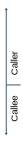
\includegraphics[width=2em]{caller_callee}}
\end{frame}

\begin{frame}{Typical Return Sequence}
	\begin{enumerate}
	\item The callee places the return value next to the parameters.
	\item Using information in the machine-status fields, the callee restores \code{top\_sp} and other registers. \\
		It branches to the return address that the caller placed in the status field.
	\item Although \code{top\_sp} has been decremented, the caller knows where the return value is, relative to the current value of \code{top\_sp}. \\
		The caller may use that value.
	\end{enumerate}
	\putat(-20,-172){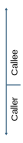
\includegraphics[width=2em]{callee_caller}}
\end{frame}

\subsubsection{Variable-length data on the stack}

\tableofcontentslide[sections={1-4},sectionstyle={show/shaded},subsectionstyle={show/shaded/hide},subsubsectionstyle={show/shaded/hide/hide}]

\begin{frame}{Variable-length Data}
	\begin{itemize}
	\item Programs contain a lot of data whose \Emph{sizes are known at run-time}; but which are local to a procedure.
	\item Because \Emph{they are local to the procedure}, they may be allocated on the stack.
	\vfill
	\item In most of the modern languages, these objects are allocated in the \emph{heap}.
	\item However, it is also possible to allocate objects, arrays, or other data structures of unknown size on the \emph{stack}.
	\end{itemize}
	\vfill
	\begin{block}{Why on the stack?}
		Avoiding the expense of garbage collecting the space allocated for the variable-length data.
	\end{block}
\end{frame}

\pgfdeclareimage[width=.3\paperwidth]{stack_allocation_strategy}{imgs/chapter5/stack_allocation_strategy}

\begin{frame}[fragile]{Allocation Strategy}
	\putat(180,-140){\pgfuseimage{stack_allocation_strategy}}
	\begin{itemize}
	\item Below, the example of programs in C99 and C\# in which a local array is declared. Its size depends on the value of the procedure parameter.
	\end{itemize}
	\begin{minipage}{.5\linewidth}
	\begin{itemize}
	\item The common strategy is to:
		\begin{enumerate}
		\item Allocate the arrays at the end of the record.
		\item Put pointers to the allocated regions in the local data.
		\end{enumerate}
	\end{itemize}
	\end{minipage} \\
	\vspace{2em}
	\begin{columns}
		\begin{column}{.5\linewidth}
			\begin{lstlisting}[language=c]
			/* C99 */
			void myFunction(int n) {
			   float localArray[n];
			   /* Do something with array */
			}
			\end{lstlisting}
		\end{column}
		\begin{column}{.5\linewidth}
			\begin{lstlisting}[language=c]
			/* C# */
			unsafe void myFunction(int n) {
			   int* localArray = stackalloc int[size];
			   /* Do something with array */
			}
			\end{lstlisting}
		\end{column}
	\end{columns}
\end{frame}

\begin{frame}{Pointers \code{top} and \code{top\_sp}}
	\begin{itemize}
	\item Two pointers are used:
		\begin{description}
		\item[top] marks the actual top of the stack. It points to the position at which the next activation record will begin.
		\item[top\_sp] is used to find local, fixed-length fields of the top activation record.
		\end{description}
	\vfill
	\item When returning from a call: \\
		\code{top $\leftarrow$ top\_sp - length(fixed\_record\_part)}
	\end{itemize}
	\vfill
	\begin{center}
		\pgfuseimage{stack_allocation_strategy}
	\end{center}
\end{frame}

\subsection{Access to nonlocal data on the stack}

\subsubsection{Introduction}

\tableofcontentslide[sections={1-4},sectionstyle={show/shaded},subsectionstyle={show/shaded/hide},subsubsectionstyle={show/show/hide/hide}]

\begin{frame}{Access to Nonlocal Data on the Stack}
	\begin{itemize}
	\item This section is devoted to the mechanisms of the procedures to access to their data.
	\item Focusing on the mechanisms for finding data used within a procedure p but that does not belong to p.
	\vfill
	\item First, we study the cases of programs without nested functions.
	\item Second, we introduces an algorithmic languages that permits to declare nested functions.
	\end{itemize}
\end{frame}

\subsubsection{Data access without nested procedure}

\tableofcontentslide[sections={1-4},sectionstyle={show/shaded},subsectionstyle={show/shaded/hide},subsubsectionstyle={show/shaded/hide/hide}]

\begin{frame}{Data Access Without Nested Procedures}
	\begin{itemize}
	\item In languages similar to C, variables are declared:
		\begin{itemize}
		\item inside a single function, or
		\item outside any function (``globally'')
		\end{itemize}
	\vfill
	\item It is impossible to declare a procedure inside the scope of another procedures.
	\vfill
	\item In such languages, allocation of storage for, and access to variables is simple:
		\begin{itemize}
		\item \emph{Global variables are allocated in the static storage.} The locations remain fixed and are known at compile time.
		\item \emph{Any other name must be local to the activation at the top of the stack.} The locations are relative to the \code{top\_sp} pointer of the stack.
		\end{itemize}
	\end{itemize}
\end{frame}

\subsubsection{Issues with nested procedures}

\tableofcontentslide[sections={1-4},sectionstyle={show/shaded},subsectionstyle={show/shaded/hide},subsubsectionstyle={show/shaded/hide/hide}]

\begin{frame}[fragile]{Language with Nested Procedure Declarations}
	\begin{itemize}
	\item Many languages enable to declare procedures inside the scope of another procedure (Algol60, Pascal, ML, LISP).
	\item LISP is a functional language: variables, after initialized cannot change.
	\end{itemize}
	\vfill
	\begin{columns}
		\begin{column}{.4\linewidth}
			Factorial Function, non-tail-recursion algorithm. \\
			\vspace{3em}
			Factorial Function, tail-recursion algorithm.
		\end{column}
		\begin{column}{.6\linewidth}
			\begin{lstlisting}[language=lisp,basicstyle=\footnotesize]
			(deffun factorial (n)
				(if (<= n 1)
				    1
				    (* n factorial (- n 1))))

			(deffun factorial (n)
				(let ((deffun fact (n,acc)
					      (if (<= n 1) acc
					          (fact (- n 1) (* n acc))))
				     (fact n 1)))
			\end{lstlisting}
		\end{column}
	\end{columns}
\end{frame}

\begin{frame}{Issue with Nested Procedures}
	\begin{footnotesize}
	\alertbox{With nested procedure declaration, it is far more complicated to determine the addresses of the names used in the procedure.}
	\vfill
	\begin{example}
		\begin{columns}
			\begin{column}[t]{.6\linewidth}
				\begin{itemize}
				\item Let the procedure \code{g} declared inside the scope of the procedure \code{p}.
				\item \code{g} is accessing to the variable \code{a}, locally declared in \code{p}.
				\item It is difficult to determine at compile time where is the variable \code{a} in the stack, because of the recursive calls.
				\item The address of \code{a} in the stack can be determined only at run-time.
				\end{itemize}
			\end{column}
			\begin{column}[t]{.4\linewidth}
				\begin{scriptsize}
				\begin{myprocedure}{p}{n}
				\Begin{
					\KwSty{Declare} a \affect n/2\;
					\KwSty{Procedure} {g()} \\
					\Begin{
						\lIf{$n>1$}{p(n-1)\;}
						\lElseIf{$n=1$}{p(a/2)\;}
					}
					g() \;
				}
				\end{myprocedure}
				\end{scriptsize}
			\end{column}
		\end{columns}
	\end{example}
	\end{footnotesize}
\end{frame}

\figureslide{Example of the Issue}{nested_procedure_issue}

\subsubsection{Nesting depth}

\tableofcontentslide[sections={1-4},sectionstyle={show/shaded},subsectionstyle={show/shaded/hide},subsubsectionstyle={show/shaded/hide/hide}]

\begin{frame}{Informal Definition of Nesting Depth}
	\begin{itemize}
	\item Let nesting depth $1$ the declaration of a procedure outside another procedure.
	\item Let nesting depth $2$ the declaration of a procedure inside one other procedure of nesting depth $1$.
	\item Let nesting depth $n$ the declaration of a procedure inside one other procedure of nesting depth $n-1$.
	\end{itemize}
	\begin{columns}
		\begin{column}{.3\linewidth}
			\begin{scriptsize}
			\begin{myprocedure}{p}{n}
			\Begin{
				\KwSty{Declare} a \affect n/2\;
				\KwSty{Procedure} {g()} \\
				\Begin{
					\lIf{$n>1$}{p(n-1)\;}
					\lElseIf{$n=1$}{p(a/2)\;}
				}
				g() \;
			}
			\end{myprocedure}
			\end{scriptsize}
		\end{column}
		\begin{column}{.35\linewidth}
			\begin{small}
			\code{p} has nesting depth $1$. \\
			\vspace{2em}
			\code{g} has nesting depth $2$.
			\end{small}
		\end{column}
	\end{columns}
\end{frame}

\subsubsection{Access links}

\tableofcontentslide[sections={1-4},sectionstyle={show/shaded},subsectionstyle={show/shaded/hide},subsubsectionstyle={show/shaded/hide/hide}]

\begin{frame}{Access Link}
	\begin{small}
	\begin{definition}
		Access links provide a mean for the implementation of the static scope rule for nested functions.
	\end{definition}
	\begin{description}
	\item If procedure \code{g} is immediately nested in procedure \code{p}; then the access link in any activation of \code{g} points to the most recent activation of \code{p}.
	\item[Note] nesting depth of \code{p} must be exactly one less than the nesting depth of \code{g}.
	\end{description}
	\end{small}
	\begin{columns}
		\begin{column}{.5\linewidth}
			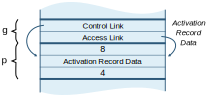
\includegraphics[width=\linewidth]{access_link}
		\end{column}
		\begin{column}{.3\linewidth}
			\begin{tiny}
			\begin{myprocedure}{p}{n}
			\Begin{
				\KwSty{Declare} a \affect n/2\;
				\KwSty{Procedure} {g()} \\
				\Begin{
					\lIf{$n>1$}{p(n-1)\;}
					\lElseIf{$n=1$}{p(a/2)\;}
				}
				g() \;
			}
			\end{myprocedure}
			\end{tiny}
		\end{column}
	\end{columns}
\end{frame}

\begin{frame}{Chain of Access Links}
	\begin{itemize}
	\item Access links form a chain from the activation record at the top of the stack to a sequence of activations at progressively lower nesting depths.
	\vfill
	\item Along this chain are all the activations whose data and procedures are accessible to the currently executing procedure.
	\end{itemize}
\end{frame}

\begin{frame}{Example of Access Links}
	\putat(160,-75){\parbox{.5\linewidth}{\normalcolor\mdseries
		\begin{tiny}
		\begin{myprocedure}{sqrt}{q}
		\Begin{
			\KwSty{Procedure} {babylonian\_algo(a,n)} \\
			\Begin{
				\KwSty{Declare} {a}\;
				b \affect (a + q/a) / 2\;
				\uIf{n {\textgreater} 0}{
					\Return {b}\;
				}
				\Else{
					\Return {babylonian\_algo(a,n-1)}\;
				}
			}
			\Return{babylonian\_algo(q/2, 10)}\;
		}
		sqrt(5)\;
		\end{myprocedure}
		\end{tiny}
	}}
	\putat(160,-170){\only<4>{\parbox{.5\linewidth}{\normalcolor\mdseries
		\small\nohyphens{To access to the value of \code{q}, we know at compile time, that it is reachable after one dereferencing in the access link pointer chain.}
	}}}
	\putat(-20,-190){\includeanimatedfigure[width=.5\paperwidth]{access_link_example}}
\end{frame}

\begin{frame}[t]{Determining the Access Link Target}
	\begin{small}
	\begin{itemize}
	\item Let the procedure \code{q} calling \code{p}.
	\item Let $N_\alpha$ the nesting depth of $\alpha$.
	\item Let $D_\beta$ the set of the nesting procedures in which $\beta$ is defined.
	\end{itemize}
	\end{small}
	\begin{block}{First Case}
		\[ \left( N_p > N_q \right) \Rightarrow \left( q \in D_p \wedge N_p = N_q + 1 \right) \]
		Then the access link from \code{p} leads to \code{q}.
	\end{block}
\end{frame}

\begin{frame}[t]{Determining the Access Link Target}
	\begin{small}
	\begin{itemize}
	\item Let the procedure \code{q} calling \code{p}.
	\item Let $N_\alpha$ the nesting depth of $\alpha$.
	\item Let $D_\beta$ the set of the nesting procedures in which $\beta$ is defined.
	\end{itemize}
	\end{small}
	\begin{block}{Second Case}
		\[ \left( N_p \le N_q \right) \Rightarrow \left( \exists r \; \bigg| \; \begin{pmatrix}
			r \in D_p \wedge N_p = N_r + 1 \wedge \\
			r \in D_q \wedge N_r > N_q
			\end{pmatrix} \right) \]
		Then \begin{itemize}
			\item The access link from \code{p} leads to \code{r}.
			\item There is $N_q - N_p + 1$ access links from \code{q} to \code{r}.
			\item Include recursive calls, where \code{p} = \code{q}.
			\end{itemize}
	\end{block}
\end{frame}

\begin{frame}[t]{Passing a Procedure as Parameter}
	\begin{itemize}
	\item A procedure \code{p} is passed to another procedure \code{q} as a parameter; \code{q} calls its parameter.
	\end{itemize}
	\begin{alertblock}{Problem}
		\begin{itemize}
		\item If \code{q} does not know the context in which \code{p} appears in the program;
		\item it is impossible for \code{q} to know how to set the access link for \code{p}.
		\end{itemize}
	\end{alertblock}
	\begin{block}{Solution}
		\begin{itemize}
		\item The caller of a procedure with a procedure as parameter must also pass the proper access link to the parameter
		\item ie. the caller must pass the name and the access link as parameters.
		\end{itemize}
	\end{block}
\end{frame}

\begin{frame}[fragile]{Example of a Procedure Passing as Parameter}
	\putat(172,-74){\parbox{.5\linewidth}{\normalcolor\mdseries
		\begin{tiny}
			{{\def\dash{\raise2.1pt\hbox{\rule{1pt}{0.3pt}}\hspace{1pt}}\begin{tabbing}
			({\textbf{defun}}\ a(x)\\
			\makebox[16pt][l]{}\makebox[16pt][l]{({\textbf{let}}\ (}({\textbf{defun}}\ b(f)\\
			\makebox[16pt][l]{}\makebox[16pt][l]{}\makebox[16pt][l]{}(\dots\ f\ \dots)\\
			\makebox[16pt][l]{}\makebox[16pt][l]{})\\
			\makebox[16pt][l]{}\makebox[16pt][l]{}({\textbf{defun}}\ c(y)\\
			\makebox[16pt][l]{}\makebox[16pt][l]{}\makebox[16pt][l]{}\makebox[16pt][l]{({\textbf{let}}\ (}({\textbf{defun}}\ d(z)\ (\dots))\ )\\
			\makebox[16pt][l]{}\makebox[16pt][l]{}\makebox[16pt][l]{}\ \ \ \ \ \ (\dots\ (b\ d)\ \dots)\\
			\makebox[16pt][l]{}\makebox[16pt][l]{}\makebox[16pt][l]{})\\
			\makebox[16pt][l]{}\makebox[16pt][l]{})\\
			\makebox[16pt][l]{}\ \ \ \ \ )\\
			\makebox[16pt][l]{}\ \ \ \ \ (\dots\ (c\ 1)\ \dots)\\
			\makebox[16pt][l]{})\\
			)
			\end{tabbing}}}
		\end{tiny}
	}}
	\only<1>{\putat(160,-170){\parbox{.5\linewidth}{\normalcolor\mdseries\small\nohyphens{Function \code{a} is called.}}}}
	\only<2>{\putat(160,-170){\parbox{.5\linewidth}{\normalcolor\mdseries\small\nohyphens{Function \code{c} is called.\\According to the first case, access link leads to \code{a}.}}}}
	\only<3>{\putat(160,-170){\parbox{.5\linewidth}{\normalcolor\mdseries\small\nohyphens{Function \code{b} is called with the procedure \code{d} as parameter.\\According to the second case, access link leads to \code{a}.\\The context of \code{d} is also passed as parameter.}}}}
	\only<4>{\putat(160,-170){\parbox{.5\linewidth}{\normalcolor\mdseries\small\nohyphens{Function \code{d} is called through the parameter \code{f}. The access link is directly taken from the context \textcircledP.}}}}
	\putat(-20,-190){\includeanimatedfigure[width=.5\paperwidth]{procedure_as_parameter_example}}
\end{frame}

\subsubsection{Displays}

\tableofcontentslide[sections={1-4},sectionstyle={show/shaded},subsectionstyle={show/shaded/hide},subsubsectionstyle={show/shaded/hide/hide}]

\begin{frame}{Problem with Access Links}
	\alertbox{If the nesting depth gets large, we may have to follow long chains of links to reach the data we need.}
\end{frame}

\sidecite{Dijkstra.1960}
\begin{frame}{The Display: a Solution to the Access Link Problem}
	\alertbox*{Use of an auxiliary array \code{d}, called the \emph{display}.}
	\vfill
	\begin{itemize}
	\item A display is a collection (an array) of pointers, one for each nesting depth.
	\vfill
	\item At all times, \code{d[i]} is a pointer to the highest activation record on the stack for any procedure at nesting depth \code{i}.
	\end{itemize}
\end{frame}

\begin{frame}{Why Displays?}
	\begin{itemize}
	\item If procedure \code{p} is executing, and it needs to access element \code{x} belonging to some procedure \code{q}, we need to look only in \code{d[i]}, where \code{i} is the nesting depth of \code{q}.
	\vfill
	\item The compiler knows what \code{i} is, so it can generate code to access \code{x} using \code{d[i]} and the offset of \code{x} from the top of the activation record for \code{q}.
	\vfill
	\item The code never needs to follow a long chain of access links.
	\end{itemize}
\end{frame}

\begin{frame}{Maintaining the Displays when Creating Records}
	\begin{itemize}
	\item Each time a record is added in the stack, we need to save previous values of display entries.
	\vfill
	\item \Emph{If} procedure \code{p} at depth $N_p$ is called, \Emph{and}
	\item the activation record of \code{p} is not the first on the stack for a procedure at depth $N_p$, \Emph{then}
	\vfill
	\item Put the value of \code{d[$N_p$]} in the activation record of \code{p}.
	\item Set \code{d[$N_p$]} to the activation record of \code{p}.
	\end{itemize}
\end{frame}

\begin{frame}{Maintaining the Displays when Returning from Records}
	\begin{itemize}
	\item Each time a record returns, we need to restore previous values of display entries.
	\vfill
	\item Set \code{d[$N_p$]} to the value previously stored in the activation record of \code{p}.
	\end{itemize}
\end{frame}

\begin{frame}[fragile]{Example of Displays}
	\putat(172,-74){\parbox{.5\linewidth}{\normalcolor\mdseries
		\begin{tiny}
			{{\def\dash{\raise2.1pt\hbox{\rule{1pt}{0.3pt}}\hspace{1pt}}\begin{tabbing}
			({\textbf{defun}}\ a(x)\\
			\makebox[16pt][l]{}\makebox[16pt][l]{({\textbf{let}}\ (}({\textbf{defun}}\ b(f)\\
			\makebox[16pt][l]{}\makebox[16pt][l]{}\makebox[16pt][l]{}(\dots\ f\ \dots)\\
			\makebox[16pt][l]{}\makebox[16pt][l]{})\\
			\makebox[16pt][l]{}\makebox[16pt][l]{}({\textbf{defun}}\ c(y)\\
			\makebox[16pt][l]{}\makebox[16pt][l]{}\makebox[16pt][l]{}\makebox[16pt][l]{({\textbf{let}}\ (}({\textbf{defun}}\ d(z)\ (\dots))\ )\\
			\makebox[16pt][l]{}\makebox[16pt][l]{}\makebox[16pt][l]{}\ \ \ \ \ \ (\dots\ (b\ d)\ \dots)\\
			\makebox[16pt][l]{}\makebox[16pt][l]{}\makebox[16pt][l]{})\\
			\makebox[16pt][l]{}\makebox[16pt][l]{})\\
			\makebox[16pt][l]{}\ \ \ \ \ )\\
			\makebox[16pt][l]{}\ \ \ \ \ (\dots\ (c\ 1)\ \dots)\\
			\makebox[16pt][l]{})\\
			)
			\end{tabbing}}}
		\end{tiny}
	}}
	
	\only<1>{\putat(170,-170){\parbox{.5\linewidth}{\normalcolor\mdseries\small\nohyphens{
				The displays are pointing somewhere in the stack. \\
				Function \code{a} is called. \\
				Create the record. \\
				Save \code{d[1]}, which is pointing on a lower activation record.}}}}
	\only<2>{\putat(170,-170){\parbox{.5\linewidth}{\normalcolor\mdseries\small\nohyphens{
				Because \code{d[1]} is not pointing to the record of \code{a}, change \code{d[1]}.}}}}
	\only<3>{\putat(170,-170){\parbox{.5\linewidth}{\normalcolor\mdseries\small\nohyphens{
				The function \code{c} is called. \\
				Its record is created. \\
				The previous value of \code{d[2]} is saved.}}}}
	\only<4>{\putat(170,-170){\parbox{.5\linewidth}{\normalcolor\mdseries\small\nohyphens{
				Because the record of \code{c} is not the one pointed by \code{d[2]}, set \code{d[2]} to leads to \code{c}.}}}}
	\only<5>{\putat(170,-170){\parbox{.5\linewidth}{\normalcolor\mdseries\small\nohyphens{
				The function \code{b} is called. \\
				Save the \code{d[2]}, and set its value to leads to \code{b}.}}}}
	\only<6>{\putat(170,-170){\parbox{.5\linewidth}{\normalcolor\mdseries\small\nohyphens{
				The function \code{d} is called through the parameter \code{f}. \\
				The displays are updated.}}}}
	\only<7>{\putat(170,-170){\parbox{.5\linewidth}{\normalcolor\mdseries\small\nohyphens{
					To obtain the value of \code{x}:
					\begin{itemize}\normalcolor\mdseries\small
					\item Because \code{x} is at nesting depth 1, follows \code{d[1]} to reach the right record.
					\item Read the value of \code{x} in the record.
					\end{itemize}}}}}
	\putat(-20,-190){\includeanimatedfigure[width=.5\paperwidth]{display_example}}
\end{frame}

\section{Heap management}

\tableofcontentslide[sections={1-5},sectionstyle={show/shaded},subsectionstyle={show/show/hide},subsubsectionstyle={hide/hide/hide/hide}]

\subsection{Introduction}

\begin{frame}{What is the Heap?}
	\begin{itemize}
	\item The heap is the portion of the store that is used for data that lives indefinitely, or until the program explicitly deletes it.
	\vfill
	\item Modern languages provides dedicated operators for the allocation and deallocation in the heap. For example, \kw{new} and \kw{delete} in C++.
	\end{itemize}
\end{frame}

\begin{frame}{Heap Management}
	\begin{itemize}
	\item This section describes the \emph{memory manager}, the subsystem that allocates and deallocates space within the heap.
	\vfill
	\item The memory manager is the interface between the application program and the operating system.
	\vfill
	\item \emph{Garbage collection} is the process of finding spaces within the heap that are no longer used by the program and can be reallocated. The \emph{garbage collector} is an important subcomponent of the memory manager.
	\end{itemize}
\end{frame}

\subsection{Memory manager}

\tableofcontentslide[sections={1-5},sectionstyle={show/shaded},subsectionstyle={show/shaded/hide},subsubsectionstyle={hide/hide/hide/hide}]

\begin{frame}{Memory Manager}
	\begin{itemize}
	\item The memory manager keeps track of all the free space in heap storage at all times.
	\vfill
	\item Its two basic functions are:
		\begin{enumerate}
		\item allocation,
		\item deallocation.
		\end{enumerate}
	\end{itemize}
\end{frame}

\begin{frame}{Allocation by the Memory Manager}
	\begin{itemize}
	\item Produces a chunk of contiguous memory for each variable or object associated to the allocation request.
	\vfill
	\item If not enough contiguous space is available for a chunk, it seeks to increase the heap storage space by requesting memory to the operating system.
	\vfill
	\item The defragmentation of the heap is generally not implemented.
	\end{itemize}
\end{frame}

\begin{frame}{Deallocation by the Memory Manager}
	\begin{itemize}
	\item Returns deallocated space to the pool of free space.
	\vfill
	\item The deallocation space may be reused for future allocations.
	\vfill
	\item Typically, the memory manager does not return memory to the operating system, even if the program's heap usage drops.
	\end{itemize}
\end{frame}

\begin{frame}{Space Efficiency of the Memory Manager}
	\begin{block}{Property: Space Efficiency}
		\begin{itemize}
		\item A memory manager should minimize the total heap space need by a program.
		\item Space efficiency is achieved by minimizing the ``fragmentation'' (discussed later).
		\end{itemize}
	\end{block}
\end{frame}

\begin{frame}{Program Efficiency of the Memory Manager}
	\begin{block}{Property: Program Efficiency}
		\begin{itemize}
		\item A memory manager should make good use of the memory subsystem to allow programs to run faster.
		\item The time taken to execute an instruction can vary widely depending on where objects are placed in memory.
		\item Programs tends to exhibit ``locality'' (discussed later), which refers to the nonrandom clustered way in which typical programs access memory.
		\item By attention to the placement of objects in memory, the memory manager can make better use of space, and make the program run faster.
		\end{itemize}
	\end{block}
\end{frame}

\begin{frame}{Low Overhead of the Memory Manager}
	\begin{block}{Property: Low Overhead}
		\begin{itemize}
		\item Because memory allocations and deallocations are frequent operations in many programs (such as ones written in Java), it is important that these operations be as efficient as possible.
		\item We wish to minimize the overhead, the fraction of execution time spent performing allocation and deallocation.
		\end{itemize}
	\end{block}
	\vspace{1em}
	\begin{description}
	\item[Note] the overhead of allocation is dominated by a large amount of small requests; the overhead of managing large objects is less important.
	\end{description}
\end{frame}

\begin{frame}{Efficiency of a Program}
	\begin{itemize}
	\item The efficiency of a program is determined by:
		\begin{enumerate}
		\item the number of instructions executed, and
		\item the time taken to execute each of these instructions.
		\end{enumerate}
	\vfill
	\item Data-intensive programs can therefore benefit significantly from optimizations that make good use of the memory subsystem.
	\vfill
	\item \emph{The run-time environment should prefer to use the memory storages close to the processor.}
	\vfill
	\item The concept of ``locality'' will help us to improve the use of the memory subsystem.
	\end{itemize}
\end{frame}

\subsection{Locality in programs}

\tableofcontentslide[sections={1-5},sectionstyle={show/shaded},subsectionstyle={show/shaded/hide},subsubsectionstyle={hide/hide/hide/hide}]

\begin{frame}{Concept of Locality}
	\begin{small}
	\begin{block}{\small Hypothesis}
		The conventional wisdom is that programs spend 90\% of their time executing 10\% of the code.
	\end{block}
	In other words: they spend most of their time executing a relatively small fraction of the code and touching only a small fraction of the data.
	\begin{definition}[Temporal Locality]
		The memory locations, which are accessed by the program, are likely to be accessed again within a short period of time.
	\end{definition}
	\begin{definition}[Spatial Locality]
		The memory locations close to the accessed location are likely also to be accessed within a short period of time.
	\end{definition}
	\end{small}
\end{frame}

\begin{frame}{Consequences of the Locality}
	\begin{enumerate}
	\item Programs often contains many instructions that are never executed.
	\vfill
	\item After evolution, legacy systems contain many instructions that are no longer used.
	\vfill
	\item Only a small fraction of the code that could be invoked is actually executed in a typical run of the program.
	\vfill
	\item The typical program spends most of its time executing innermost loops and tight recursive cycles in a program.
	\end{enumerate}
\end{frame}

\begin{frame}{Memory Hierarchy}
	\begin{itemize}
	\item Memory manager (and compiler optimizer) must be aware of how the operating system is managing its memory.
	\item In modern systems, the memory is composed of several layers:
	\end{itemize}
	\vspace{1em}
	\begin{center}
	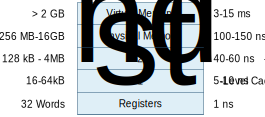
\includegraphics[width=.8\linewidth]{memory_hierarchy}
	\end{center}
\end{frame}

\begin{frame}{Locality and Memory Hierarchy}
	\begin{itemize}
	\item Locality permits to take advantage of the memory hierarchy.
	\vfill
	\item By placing the most common instructions and data in the fast-but-small storage, 
	\vfill
	\item While leaving the rest in the slow-but-large storage, we can lower the average memory-access time.
	\end{itemize}
\end{frame}

\begin{frame}{Optimization Policy}
	\begin{small}
	\begin{itemize}
	\item Put the most-recent-used instruction in the fastest memory (example of spatial locality).
	\item Put together in the same memory page/block the instructions that may be always executed together (example of spatial locality).
	\item Temporal and spatial locality of data be improved by changing:
		\begin{itemize}
		\item the data layout, or
		\item the order of the computations.
		\end{itemize}
	\end{itemize}
	\begin{example}
		\begin{itemize}
		\item For example, visiting a large amount of data and performing small operations on is not a good approach.
		\item Preferably, we should push down smaller data set into a faster memory level, and perform the computations on them.
		\end{itemize}
	\end{example}
	\end{small}
\end{frame}

\subsection{Reduction of the fragmentation}

\tableofcontentslide[sections={1-5},sectionstyle={show/shaded},subsectionstyle={show/shaded/hide},subsubsectionstyle={hide/hide/hide/hide}]

\begin{frame}{Holes in the Heap}
	\begin{itemize}
	\item At the beginning of the program, the heap is one contiguous unit of free space.
	\vfill
	\item As the program allocates and deallocates memory, this space is broken up into free and used chunks.
	\vfill
	\item The free chunks need not reside in a contiguous area of the heap.
	\vfill
	\item \emph{The free chunks are named holes.}
	\vfill
	\item Alternating chunks and holes is named the \emph{fragmentation} of the heap.
	\end{itemize}
\end{frame}

\begin{frame}{Object Placement for Minimizing the Defragmentation}
	\begin{itemize}
	\item We reduce fragmentation by controlling how the memory manager places new objects in the heap.
	\vfill
	\item Several approaches/strategies may be used:
		\vfill
		\begin{enumerate}
		\item[Best-Fit Object Placement] Allocate the requested memory in the smallest available hole that is large enough. Not good for spatial locality.
		\vfill
		\item[First-Fit Object Placement] Allocate the requested memory in the first hole, which is able to contains the requested chunk. Less efficient than the previous one.
		\vfill
		\item[Next-Fit Object Placement] When no hole of the exact size was found, allocate the in the lastly split hole. Good for spatial locality and efficient.
		\end{enumerate}
	\end{itemize}
\end{frame}

\begin{frame}{Bins in the Best-Fit Implementation}
	\begin{itemize}
	\item To improve the implementation of the best-fit approach, we introduces the \emph{bins}.
	\item \emph{Free space chunks are grouped into bins}, according to their sizes.
	\item Many bins for the smaller sizes, because there are usually many more small objects.
	\end{itemize}
	\begin{block}{\small Lea Memory Manager (GNU C compiler)}\small 
		\begin{itemize}
		\item Bins of every multiple of 8 bytes until 512 bytes.
		\item Larger-sized bins are logarithmically spaced.
		\item Within the bins the chunks are ordered by their sizes.
		\item Wilderness chunk: the largest bin because its size may be extended after requesting more memory to OS.
		\end{itemize}
	\end{block}
\end{frame}

\begin{frame}{Allocation of a Chunk}
	Let a requested chunk \code{c} to be allocated.
	\begin{enumerate}
	\item If there is a bin for chunks of the size of \code{c}, we take any free space chunk from that bin.
	\vfill
	\item\label{allocation_chunk_b} If there is no bin for chunks of the size of \code{c}, we take the smallest bin that may include the requested size. \\
		Within that bin, we can use either a first-fit or a best-fit strategy. \\
		The remainder space of the selected chunk will generally be placed in a bin with smaller size.
	\vfill
	\item If there is no more free chunk in a bin, we repeat the point \ref{allocation_chunk_b} on a bin for a larger size; or we reach the wilderness chunk, which surely provide enough space.
	\end{enumerate}
\end{frame}

\begin{frame}{Managing and Coalescing Free Space}
	\begin{itemize}
	\item When an object is deallocated, the memory manager make its chunk free.
	\item In some circumstances, it may also be possible to combine (coalesce) that freed chunk with adjacent chunks.
	\vfill
	\item Two majors data structures are basically used for supporting coalescing of adjacent free blocks:
		\begin{enumerate}
		\item \emph{Boundary Tags},
		\item \emph{Doubly Linked Free List}, Embedded Free List.
		\end{enumerate}
	\end{itemize}
\end{frame}

\sidecite{Knuth.1968}
\begin{frame}{Boundary Tags}
	\sidenote{The order of the boundary tags depends on the run-time environment}
	\begin{itemize}
	\item At both the low and high ends of a chunk, whether free or allocated, we keep vital information.
	\vfill
	\item \Emph{At both ends}, we put:
		\begin{enumerate}
		\item a bit that indicates if the chunk is free or allocated.
		\item a count of the total number of bytes in the chunk.
		\end{enumerate}
	\end{itemize}
	\vfill
	\begin{center}
		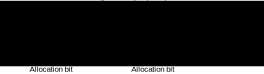
\includegraphics[width=.8\linewidth]{boundary_tags}
	\end{center}
\end{frame}

\begin{frame}{Doubly Linked Free List}
	\sidenote{The order of the boundary tags depends on the run-time environment}
	\begin{itemize}
	\item The free chunks (but not the allocated ones) are linked in a doubly linked list.
	\vfill
	\item In addition to the boundary tags, a pointer to the next and to the following free space chunks are added at the both ends of the chunk.
	\vfill
	\item Does not need to allocate more space for these pointers: the pointers takes the unused bytes of the free chunks.
	\item For the smaller chunks, they are expanded to allow to contain the pointers.
	\end{itemize}
	\vfill
	\begin{center}
		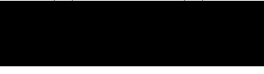
\includegraphics[width=.8\linewidth]{doubly_linked_list}
	\end{center}
\end{frame}

\subsection{Manual Deallocation}

\tableofcontentslide[sections={1-5},sectionstyle={show/shaded},subsectionstyle={show/shaded/hide},subsubsectionstyle={hide/hide/hide/hide}]

\begin{frame}{Manual Deallocation}
	\begin{itemize}
	\item This subsection is devoted to the manual deallocation requests, such as in C and C++ languages.
	\vfill
	\item Ideally, any storage that will no longer be accessed should be deleted.
	\vfill
	\item Conversely, any storage that may be referenced must not be deleted.
	\vfill
	\item It is hard to enforce these properties.
	\end{itemize}
\end{frame}

\begin{frame}{Main Problems with Manual Deallocations}
	Two common errors may occurs in manual memory management:
	\begin{enumerate}
	\vfill
	\item[Memory Leak] failing ever to delete data that cannot be referenced.
	\vfill
	\item[Dangling-pointer reference] referencing deleted data.
	\end{enumerate}
\end{frame}

\begin{frame}{Problem of Memory Leak}
	\begin{small}
	\begin{block}{\small Observation}
		\begin{itemize}
		\item It is hard for a developer to tell if a program will never refer to some storage in the future.
		\item The common mistake is not deleting storage that will never be referenced.
		\end{itemize}
	\end{block}
	\begin{alertblock}{\small Problem}
		May slow down the execution of the program due to increased memory usage.
	\end{alertblock}
	\begin{block}{\small Remarks}
		\begin{itemize}
		\item Correctness of the program is not changed.
		\item Many programs may tolerate leaks but not the long-time and the critical ones (operating systems, server code\dots)
		\end{itemize}
	\end{block}
	\end{small}
\end{frame}

\begin{frame}{Solving the Memory Leak Problem}
	\begin{enumerate}
	\item \emph{Automatic garbage collection gets rid of memory leaks by deallocating all the garbage.}\\
		Even with a garbage collector, programs may still use more memory than necessary.
	\vfill
	\item \emph{A programmer may know that an object will never be referenced.} \\
		He must deliberately remove the references to objects that will never be referenced, so the objects can be deallocated automatically.
	\end{enumerate}
\end{frame}

\begin{frame}{Problem of Dangling-Pointer Reference}
	\begin{small}
	\begin{block}{\small Observation}
		\begin{itemize}
		\item Deletion of a storage, and then referencing the deleted storage.
		\item These pointers are named ``dangling pointers.''
		\end{itemize}
	\end{block}
	\begin{alertblock}{\small Problem}
		\begin{itemize}
		\item When the storage has been reallocated, it produces random effects on the program.
		\item Writing through a dangling pointer changes an other variable than the one expecting by the dangling pointer.
		\end{itemize}
	\end{alertblock}
	\begin{block}{\small Remarks}
		Read, write or deallocate a pointer is named ``dereferencing the pointer.''
	\end{block}
	\end{small}
\end{frame}

\begin{frame}{Solving the Dangling-Pointer-Reference Problem}
	\alertbox{Unfortunately, there is no turnkey solution.}
	\begin{enumerate}
	\item \emph{The programmer must be aware and may pay attention to his uses of the pointers.}
	\vfill
	\item \emph{The dangling-pointer-dereference error does not occurs in run-time environments that has an \Emph{automatic garbage collector}.}
	\end{enumerate}
\end{frame}

\begin{frame}{Illegal Address Error}
	\begin{definition}
		This error occurs when the address to dereference is null or outside the bounds of any allocated memory (including the bounds of the memory space of the process).
	\end{definition}
	\vfill
	\begin{itemize}
	\item The illegal address error is related to the dangling-pointer-dereference error.
	\item This error is at the origin of many security violations from hackers.
	\item One solution is that the compiler inserts checks with every access, to make sure it is within the bounds.
	\item The compiler optimizer may remove several of these checks when they are detected as not necessary.
	\end{itemize}
\end{frame}

\begin{frame}[allowframebreaks]{Programming Conventions and Tools}
	\begin{block}{Object Ownership}
	\begin{itemize}
	\item Associate an owner with each object at all times.
	\item The owner is usually a function.
	\item The owner is responsible for either deleting the object or for passing the object to another owner.
	\item Non-owning points may reference the object, but the object must never be deallocated through them.
	\item This convention eliminates memory leaks, and the deletion of the same object twice.
	\item This convention does not solve the dangling-point-reference problem.
	\end{itemize}
	\end{block}
	%
	\framebreak
	%
	\begin{block}{Reference Counting}
	\begin{itemize}
	\item Associate a count with each dynamically allocated object.
	\item Whenever the reference to the object is created, the counter is incremented.
	\item Whenever the reference to the object is deleted, the counter is decremented.
	\item The storage for the object is released when the counter is zero.
	\item Expensive operation.
	\item Do not work with inaccessible circular data structures.
	\end{itemize}
	\end{block}
	%
	\framebreak
	%
	\begin{block}{Region-Based Allocation}
	\begin{itemize}
	\item When objects are created to be used only within some step of a computation, we can allocate all such objects in the same region.
	\item We then delete the entire region once that computation step completes.
	\item Limited applicability.
	\item Very efficient.
	\end{itemize}
	\end{block}
\end{frame}

\section{Garbage collection}

\tableofcontentslide[sections={2-6},sectionstyle={show/shaded},subsectionstyle={show/show/hide},subsubsectionstyle={hide/hide/hide/hide}]

\subsection{Introduction}

\sidecite{Wilson.1994}
\begin{frame}{Introduction to Garbage Collection}
	\begin{itemize}
	\item Data that cannot be referenced as named garbage.
	\item \Emph{Many high-level programming languages remove the burden of manual memory management from the programmer by offering automatic garbage collection.}
	\item The garbage collection (GC) is the process to deallocate no-more referenced storages from the heap.
	\vfill
	\item The first garbage collection dates from the initial implementation of LISP in 1958.
	\item Other languages provide natively a GC: Java, Perl, ML, Modula-3, Prolog, Smalltalk, C\#, Ruby, Python\dots
	\end{itemize}
\end{frame}

\begin{frame}{Hypothesis for Garbage Collection}
	\begin{itemize}
	\item The garbage collector must know the type of the objects at run-time. This type permits to determine:
		\begin{enumerate}
		\item the size of the object in bytes.
		\item its components that are references to other objects.
		\end{enumerate}
	\vfill
	\item The references to the objects are always to the address of the beginning of these objects.
	\item All the references to the same object have the same value and may be identified easily.
	\end{itemize}
\end{frame}

\begin{frame}{Mutator and Garbage Collection}
	\begin{definition}[Mutator]
		The mutator, the user program, modifies the collection of objects in the heap
	\end{definition}
	\vfill
	\begin{itemize}
	\item The mutator creates objects by acquiring space from the memory manager.
	\item The mutator may introduce and drop references to existing objects.
	\item Objects become garbage when the mutator program cannot ``reach'' them.
	\item The GC finds the unreachable objects and reclaims their space by handling them to the memory manager.
	\end{itemize}
\end{frame}

\subsection{Properties of a garbage collector}

\tableofcontentslide[sections={2-6},sectionstyle={show/shaded},subsectionstyle={show/shaded/hide},subsubsectionstyle={hide/hide/hide/hide}]

\begin{frame}{Type Safety}
	\begin{itemize}
	\item For a GC to work, \emph{the language must be type safe}. \\[.5em]
		The type of the data may be determined at compile or run-time.
	\vfill
	\item GC must be able to tell whether any given data element or component of a data element is, could be used as, a pointer to a chunk.
	\vfill
	\item Two family of type-safe languages:
		\begin{enumerate}
		\item[Statically typed languages] the types are determined at compile time (ML\dots)
		\item[Dynamically typed languages] the types are determined at run-time (Java\dots)
		\end{enumerate}
	\end{itemize}
\end{frame}

\begin{frame}{Unsafe Language}
	\begin{itemize}
	\item \Emph{Unsafe languages (C, C++\dots) are bad candidate for GC.}
	\vfill
	\item In unsafe languages, memory addresses can be manipulated arbitrarily (pointer arithmetic\dots)
	\vfill
	\item Thus programs can refer to any location in memory at any time.
	\vfill
	\item Consequently, no memory location can be considered to be inaccessible, and no storage can ever be reclaimed safely.
	\end{itemize}
\end{frame}

\begin{frame}{Performance Metrics}
	\begin{footnotesize}
	\begin{description}
	\item[Overall Execution Time] It is important that GC is not significantly increase the total run time of an application.
	\vfill
	\item[Space Usage] The GC must avoid fragmentation and make the best use of the available memory.
	\vfill
	\item[Pause Time] Simple GC causes the mutator to pause suddenly for an extremely long time. \\
		The maximum pause time must be minimized.
	\vfill
	\item[Program Locality] \begin{itemize}
		\item The speed of the GC cannot be evaluated solely by its running time.
		\item The GC controls the placement of data and thus influences the data locality of the mutator program.
		\item GC can improve the mutator's temporal locality by freeing the space and reusing it.
		\item It can improve the mutator's spatial locality by relocating data used together in the same cache or pages.
		\end{itemize}
	\end{description}
	\end{footnotesize}
\end{frame}

\subsection{Reachability of data}

\tableofcontentslide[sections={2-6},sectionstyle={show/shaded},subsectionstyle={show/shaded/hide},subsubsectionstyle={hide/hide/hide/hide}]

\begin{frame}{Root Set}
	\begin{definition}
		It refer to all the data that can be accessed directly by a program, without having to dereference any pointer.
	\end{definition}
	\vfill
	\begin{example}
		In Java, the root set is composed of all the static fields and all the variables in the stack.
	\end{example}
	\vfill
	\begin{description}
	\item A program can \emph{reach} any member of its root set at any time.
	\item Recursively, any object with a reference that is stored in the field members or array elements of any reachable object is itself reachable.
	\item[Note] when an object becomes unreachable, it will never be reachable again.
	\end{description}
\end{frame}

\begin{frame}[allowframebreaks]{Basic Operations to Change the Root Set}
	\begin{block}{Object allocation}
		\begin{itemize}
		\item Performed by the memory manager.
		\item The Memory manager returns a reference to each newly allocated chunk of memory.
		\item This operation adds members to the set of reachable objects.
		\end{itemize}
	\end{block}
	\begin{block}{Parameter passing and return values}
		\begin{itemize}
		\item References to objects are passed from the actual input parameter to the corresponding formal parameters; and from the returned result back to the caller.
		\item Objects pointed to by these references remain reachable.
		\end{itemize}
	\end{block}
	\begin{block}{Reference assignments}
		\begin{itemize}
		\item Assignments of the \code{x = y} (\code{x} and \code{y} are references) have two effects:
			\begin{enumerate}
			\item \code{x} is a now a reference to the object referred by \code{y}. The object referenced by \code{x} and \code{y} is reachable while \code{x} or \code{y} is reachable.
			\item The original reference of \code{x} is lost. If this lost reference is the last on the object, the object becomes unreachable.
			\end{enumerate}
		\item When an object becomes unreachable, all the reachable objects inside becomes also unreachable.
		\end{itemize}
	\end{block}
	\begin{block}{Procedure returns}
		\begin{itemize}
		\item As a procedure exists, the frame holding its local variables is popped off the stack.
		\item If the frame holds the only reachable reference to any object, that object becomes unreachable.
		\item If the now unreachable objects holds the only references to other objects, they too become unreachable, and so on.
		\end{itemize}
	\end{block}
\end{frame}

\begin{frame}[allowframebreaks]{Finding Unreachable Objects}
	\begin{enumerate}
	\item \emph{Transitions from reachability to unreachability are catched}, or \emph{the reachable objects are periodically located; assuming that all the other objects are not reachable}. \\[1em]
		Reference counting is an approximation of the first approach:
		\begin{itemize}
		\item A count of the reference to an object is maintained.
		\item When the count goes to zero, the object becomes unreachable (discussed in the next section).
		\end{itemize}
	%
	\framebreak
	%
	\item \emph{The reachability is computed by tracing all the references transitively}. \\[1em]
		\begin{itemize}
		\item A trace-based garbage collector starts by labeling, marking, all objects in the root set as ``reachable.''
		\item It examines iteratively all the references in reachable objects to find more reachable objects.
		\item It labels the discovered objects as ``reachable.''
		\item Once the reachable set is computed, it may find the unreachable objects.
		\item All the unreachable objects could be deallocated at the same time.
		\end{itemize}
	\end{enumerate}
\end{frame}

\subsection{Reference-counting garbage collector}

\tableofcontentslide[sections={2-6},sectionstyle={show/shaded},subsectionstyle={show/shaded/hide},subsubsectionstyle={show/show/hide/hide}]

\sidenote{Collins.1960}
\begin{frame}{Reference-Counting Garbage Collector}
	\begin{itemize}
	\item This section is devoted to a simple and imperfect garbage collector based on reference counting.
	\vspace{2em}
	\item With a reference-counting garbage collector, every object must have a field for the reference count; and maintains as described in the following slides.
	\end{itemize}
\end{frame}

\begin{frame}[allowframebreaks]{Actions of Reference-Counting GC}
	\begin{description}
	\item[Object allocation] The reference count of the new object is set to 1.
	\vspace{1em}
	\item[Parameter Passing] The reference count of each object passed into a procedure is incremented.
	\vspace{1em}
	\item[Reference Assignments] For statement \code{u=v} (\code{u} and \code{v} are references), the reference count of the object referred to by \code{v} goes up by one, and the count for the old object referred to by \code{u} goes down by one.
	%
	\framebreak
	%
	\item[Procedure Returns] As a procedure exsits, objects referred to by the local variables in its activation record have their counts decremented. If several local variables hold references to the same object, that object's count must be incremented once for each such reference.
	\vspace{1em}
	\item[Transitive Loss of Reachability] Whenever the reference count of an object becomes zero, we mist also decrement the count of each object pointed to by a reference within the object.
	\end{description}
\end{frame}

\begin{frame}<-11>[t,fragile]{Example of Reference-Counting Garbage Collector}
	\begin{lstlisting}[linewidth={.35\linewidth},language=java,basicstyle=\tiny,backgroundcolor={}]
		class Obj {
		   public Obj a = null;
		   public Obj b = null;
		}
		class Main {
		   public static void main(String[] args) {
		      Obj o1 = new Obj();
		      {
		         Obj o2 = new Obj();
		         Obj o3 = new Obj();
		         o1.b = o2;
		         o2.a = o1;
		         o2.b = o3;
		         o3.b = o1;
		      }
		   }
		}
	\end{lstlisting}
	\putat(130,-200){\includeanimatedfigure[width=.4\paperwidth]{reference_counting_exemple}}
	\only<2>{\putat(-30,-79){\pgfuseimage{rightarrow}}}
	\only<3>{\putat(-30,-94){\pgfuseimage{rightarrow}}}
	\only<4>{\putat(-30,-100){\pgfuseimage{rightarrow}}}
	\only<5>{\putat(-30,-107){\pgfuseimage{rightarrow}}}
	\only<6>{\putat(-30,-115){\pgfuseimage{rightarrow}}}
	\only<7>{\putat(-30,-121){\pgfuseimage{rightarrow}}}
	\only<8>{\putat(-30,-129){\pgfuseimage{rightarrow}}}
	\only<9>{\putat(-30,-135){\pgfuseimage{rightarrow}}}
	\only<10>{\putat(-30,-142){\pgfuseimage{rightarrow}}}
	\only<11>{\putat(130,-18){\parbox[t]{.5\paperwidth}{\normalcolor\mdseries\small\nohyphens{
		This set of objects should be garbage collected. But their counters are greater than 0. Such a situation is tantamount to a \alert{memory leak}, since this set of objects will never be deallocated.}}}}
\end{frame}

\begin{frame}<12->[t,fragile]{Solving Memory Leak with Reference-Counting Garbage Collector}
	\begin{lstlisting}[linewidth={.35\linewidth},language=java,basicstyle=\tiny,backgroundcolor={}]
		class Obj {
		   public Obj a = null;
		   public Obj b = null;
		}
		class Main {
		   public static void main(String[] args) {
		      Obj o1 = new Obj();
		      {
		         Obj o2 = new Obj();
		         Obj o3 = new Obj();
		         o1.b = o2;
		         o2.a = o1;
		         o2.b = o3;
		         o3.b = o1;
		      }
		      o1.b = null;
		   }
		}
	\end{lstlisting}
	\putat(130,-200){\includeanimatedfigure[width=.4\paperwidth]{reference_counting_exemple}}
	\only<12-13>{\putat(-30,-143){\pgfuseimage{rightarrow}}}
	\only<14>{\putat(-30,-150){\pgfuseimage{rightarrow}}}
	\only<12>{\putat(130,-18){\parbox[t]{.5\paperwidth}{\normalcolor\mdseries\small\nohyphens{
		A line is added to reset the reference from \code{o1} to \code{o2}.}}}}
	\only<15>{\putat(130,-18){\parbox[t]{.5\paperwidth}{\normalcolor\mdseries\small\nohyphens{
		The chunk, previously refered by \code{o2}, is no more referenced. It is garbage collected.}}}}
	\only<16>{\putat(130,-18){\parbox[t]{.5\paperwidth}{\normalcolor\mdseries\small\nohyphens{
		Chunk refered by \code{o3} is garbage collected.}}}}
	\only<17>{\putat(130,-18){\parbox[t]{.5\paperwidth}{\normalcolor\mdseries\small\nohyphens{
		Chunk refered by \code{o1} is garbage collected. There is \emph{no memory leak}.}}}}
\end{frame}

\begin{frame}{Deferred Reference Counting}
	\begin{itemize}
	\item The concept of \emph{deferred reference counting} has been proposed as a mean to eliminate the overhead associated with updating the reference counts due to stack accesses.
	\vfill
	\item Reference counts do not include references from the root set of the program.
	\item An object is not considered to be garbage until the entire root set is scanned and no reference to the object is found.
	\end{itemize}
\end{frame}

\begin{frame}{Advantages of Reference Counting}
	\begin{enumerate}
	\item Garbage Collection is performed in an \emph{incremental fashion}.
		\begin{itemize}
		\item The operations are made through the mutator's operations.
		\item Removing one reference may render a large number of objects unreachable, the operation of recursively modifying reference counts can easily be deferred and performed piecemeal across time.
		\item Reference counting is particularly attractive when timing deadlines must be met.
		\end{itemize}
	\vfill
	\item Garbage are collected immediately, keeping space usage low.
	\end{enumerate}
\end{frame}

\begin{frame}{Disadvantages of Reference Counting}
	\begin{enumerate}
	\item Reference counting cannot collect unreachable, cyclic data structures.
		\begin{itemize}
		\item Cyclic data structures are quite plausible.
		\item Data structures often point back to their parent nodes, or point to each other as cross references.
		\end{itemize}
	\vfill
	\item Overhead of reference counting is high:
		\begin{itemize}
		\item Additional operations were introduced with each reference assignment.
		\item Additional operations were introduced with each procedure call and exit.
		\item The overhead is proportional to the amount of computation in the program, and not just to the number of objects in the system.
		\end{itemize}
	\end{enumerate}
\end{frame}

\subsection{Trace-based garbage collector}

\subsubsection{Introduction}

\tableofcontentslide[sections={4-6},sectionstyle={show/shaded},subsectionstyle={show/shaded/hide},subsubsectionstyle={show/show/hide/hide}]

\sidecite{McCarthy.1960}
\begin{frame}{Trace-Based Garbage Collector}
	\begin{itemize}
	\item Instead of collecting garbage as it is created, trace-based collectors run periodically to find unreachable objects.
	\vfill
	\item Typically, we run the trace-based collector whenever the free space is exhausted or its amount drops below some threshold.
	\vfill
	\item All trace-based algorithms:
		\begin{enumerate}
		\item compute the set of reachable objects, and
		\item Take the complement of this list.
		\end{enumerate}
	\end{itemize}
\end{frame}

\begin{frame}{States of the Chunks}
	\begin{definition}[Free]
		\begin{itemize}
		\item A chunk is in the \emph{Free} state if it is ready to be allocated.
		\item A Free chunk must not hold a reachable object.
		\end{itemize}
	\end{definition}
	\begin{definition}[Allocated]
		\begin{itemize}
		\item A chunk is in the \emph{Allocated} state if it was used to store data.
		\item An allocated chunk must be in one of the three substates:
			\begin{enumerate}
			\item Unreached
			\item Unscanned
			\item Scanned
			\end{enumerate}
		\end{itemize}
	\end{definition}
	\begin{center}
		\includegraphics[width=.5\linewidth]{chunk_states}
	\end{center}
\end{frame}

\begin{frame}[t]{States of an Allocated Chunk}
	\begin{footnotesize}
	\only<1>{\begin{definition}[Unreached]
		\begin{itemize}
		\item Chunks are presumed unreachable, unless proven reachable by tracing.
		\item A chunk is in the \emph{Unreached} state at any point during garbage collection if its reachability has not yet been established.
		\item After a round of garbage collection, the state of a reachable object is reset to Unreachable to get ready for the next round (see the next states).
		\end{itemize}
	\end{definition}}
	\only<2>{\begin{definition}[Unscanned]
		\begin{itemize}
		\item A chunk is in the \emph{Unscanned} state if it is known as be reachable, but its pointers have not yet been scanned.
		\item The transition to Unscanned from Unreached occurs when we discover that a chunk is reachable.
		\end{itemize}
	\end{definition}}
	\only<3>{\begin{definition}[Scanned]
		\begin{itemize}
		\item Every Unscanned object will eventually be scanned and transition to the \emph{Scanned} state.
		\item To scan an object, we examine each of the pointers within it and follow those pointers to the objects to which they refer.
		\item A scanned object can only contain references to other scanned ot unscanned objects, never to unreached objects. Consequently, the accessible chunks are moved to the Unscanned state if they are unreachable.
		\end{itemize}
	\end{definition}}
	\end{footnotesize}
	\only<4>{\begin{itemize}
		\item At the end of its algorithm, the GC is deallocating the unreached chunks.
		\item It is setting the states of the reached chunks to ``Unreached'' for the next GC execution.
		\end{itemize}}
	\putat(50,-210){\includeanimatedfigure[width=.7\linewidth]{allocated_chunk_states}}
\end{frame}

\subsubsection{Basic mark-and-sweep collector}

\tableofcontentslide[sections={4-6},sectionstyle={show/shaded},subsectionstyle={show/shaded/hide},subsubsectionstyle={show/shaded/hide/hide}]

\sidecite{McCarthy.1960}
\begin{frame}{Mark-and-Sweep Collector}
	\begin{itemize}
	\item Mark-and-sweep collectors are \Emph{``stop-the-world''} algorithms.
	\item They find all the unreachable objects, and put them on the list of free space.
	\vfill
	\item The algorithm visits and ``marks'' all the reachable objects in the first tracing step.
	\item Then it ``sweeps'' the entire heap to free up unreachable objects.
	\end{itemize}
\end{frame}

\begin{frame}[t,allowframebreaks]{Algorithm of the Mark-and-Sweep Collector}
	\begin{footnotesize}
	\begin{myalgorithm}
	\SetKwBlock{myBeginBlock}{begin}{}
	\SetKwFunction{copyof}{copy-of}%
	\SetKwFunction{referencesin}{references\_in}%
	\Input{A root set of objects, a heap, and a free list (named \code{Free}), with all the unallocated chunks of the heap.}
	\Output{A modified \code{Free} list after all the garbage has been removed.}
	\myBeginBlock{
		\tcc{MARKING PHASE}
		Unscanned \affect \copyof{root}\;
		\ForEach{o $\in$ Unscanned}{
			reached\_bit[o] \affect false\;
		}
		\While{$\exists$ o $\in$ Unscanned}{
			Unscanned \affect Unscanned $\setminus \{ o \}$\;
			\ForEach{r $\in$ \referencesin{o}}{
				\If{$neg$ reached\_bit[r]}{
					reached\_bit[r] \affect true\;
					Unscanned \affect Unscanned $\cup \{ r \}$\;
				}
			}
		}
	}
	\end{myalgorithm}
	\end{footnotesize}
	%
	\begin{footnotesize}
	\begin{myalgorithm}
	\SetKwBlock{myEndBlock}{}{end}
	\myEndBlock{
		\tcc{SWEEPING PHASE}
		Free \affect $\emptyset$\;
		\ForEach{c $\in$ chunks}{
			\uIf{$neg$ reached\_bit[c]}{
				Free \affect Free $\cup \{ c \}$\;
			}
			\Else{
				reached\_bit[c] \affect false\;
			}
		}
	}
	\end{myalgorithm}
	\end{footnotesize}
\end{frame}

\begin{frame}{Optimizing Mark-and-Sweep Collector}
	\begin{alertblock}{Problem}
		\begin{itemize}
		\item The final step in the mark-and-sweep algorithm is expensive.
		\item Not easy way to find the unreachable objects without examining the entire heap.
		\end{itemize}
	\end{alertblock}
	\vfill
	\begin{block}{Improved Algorithm}
		\begin{itemize}
		\item \Emph{Baker's Mark-and-sweep Algorithm.}
		\item It keeps a list of all allocated objects and compute a difference between the allocated objects and the reached objects.
		\end{itemize}
	\end{block}
\end{frame}

\sidecite{Baker.1992}
\begin{frame}[t,allowframebreaks]{Baker's Algorithm of the Mark-and-Sweep Collector}
	\begin{scriptsize}
	\begin{myalgorithm}
	\SetKwBlock{myBeginBlock}{begin}{}
	\SetKwFunction{referencesin}{references\_in}%
	\Input{A root set of objects, a heap, a free list (named \code{Free}), a listo f allocated objects \code{Unreached}.}
	\Output{A modified \code{Free} and \code{Unreached} lists.}
	\myBeginBlock{
		\tcc{MARKING PHASE}
		Unscanned \affect $\emptyset$\;
		Scanned \affect $\emptyset$\;
		\ForEach{o $\in$ root $\cap$ Unreached}{
			Unreached \affect Unreached $\setminus \{ o \}$; Unscanned \affect Unscanned $\cup \{ o \}$\;
		}
		\While{$\exists$ o $\in$ Unscanned}{
			Unscanned \affect Unscanned $\setminus \{ o \}$\;
			Scanned \affect Scanned $\cup \{ o \}$\;
			\ForEach{r $\in$ \referencesin{o}}{
				\If{r $\in$ Unreached}{
					Unreached \affect Unreached $\setminus \{ r \}$\;
					Unscanned \affect Unscanned $\cup \{ r \}$\;
				}
			}
		}
	}
	\end{myalgorithm}
	\end{scriptsize}
	\begin{scriptsize}
	\begin{myalgorithm}
	\SetKwBlock{myEndBlock}{}{end}
	\myEndBlock{
		\tcc{SWEEPING PHASE}
		Free \affect Free $\cup$ Unreached\;
		Unreached \affect Scanned\;
	}
	\end{myalgorithm}
	\end{scriptsize}
\end{frame}

\subsubsection{Mark-and-compact garbage collector}

\tableofcontentslide[sections={4-6},sectionstyle={show/shaded},subsectionstyle={show/shaded/hide},subsubsectionstyle={show/shaded/hide/hide}]

\begin{frame}{Relocating Collectors}
	\begin{itemize}
	\item Relocating collectors move reachable objects around in the heap to eliminate memory fragmentation.
	\item After identifying all the holes, instead of freeing them, one alternative is to relocate the allocated objects in one end of the heap.
	\item The rest of the memory becomes a single free chunk.
	\vfill
	\item Two major approaches for building a relocating collector are:
		\begin{enumerate}
		\item A \emph{mark-and-compact collector}
		\item A \emph{copying collector}
		\end{enumerate}
	\end{itemize}
\end{frame}

\begin{frame}{Mark-and-Compact Collectors}
	The mark-and-compact collector follows:
	\vfill
	\begin{enumerate}
	\item[Marking Phase] similar to the mark-and-sweep algorithms
	\vfill
	\item[Object Relocation] \begin{itemize}
		\item The allocated regions of the heap are scanned.
		\item The address of each reachable object is computed from the low end of the heap.
		\item The addresses are stored in a structure named \code{NewLocation}.
		\end{itemize}
	\vfill
	\item[Object Copy] \begin{itemize}
		\item The objects are copied to their new locations,
		\item The references in the objects to point to are updated.
		\end{itemize}
	\end{enumerate}
\end{frame}

\begin{frame}[t,allowframebreaks]{Algorithm of the Mark-and-Compact Collector}
	\begin{footnotesize}
	\begin{myalgorithm}
	\SetKwFunction{copyof}{copy\_of}%
	\SetKwFunction{referencesin}{references\_in}%
	\SetKwBlock{myBeginBlock}{begin}{}
	\Input{A root set of objects, a heap, a pointer marking the start of the free space (named \code{Free}).}
	\Output{The new value of pointer \code{Free}}
	\myBeginBlock{
		\tcc{MARKING PHASE}
		Unscanned \affect \copyof{root}\;
		\ForEach{o $\in$ Unscanned}{
			reached\_bit[o] \affect false\;
		}
		\While{$\exists$ o $\in$ Unscanned}{
			Unscanned \affect Unscanned $\setminus \{ o \}$\;
			\ForEach{r $\in$ \referencesin{o}}{
				\If{$neg$ reached\_bit[r]}{
					reached\_bit[r] \affect true\;
					Unscanned \affect Unscanned $\cup \{ r \}$\;
				}
			}
		}
	}
	\end{myalgorithm}
	\end{footnotesize}
	\begin{footnotesize}
	\begin{myalgorithm}
	\SetKwFunction{sizeof}{size\_of}%
	\SetKwBlock{myBlock}{}{}
	\myBlock{
		\tcc{COMPUTE THE NEW LOCATIONS}
		NewLocation \affect $[]$\;
		Free \affect first address in the heap;
		\ForEach{c $\in$ chunks[0..]}{
			\If{reached\_bit[c]}{
				NewLocation[c] \affect Free\;
				Free \affect Free \sizeof{c}\;
			}
		}
	}
	\end{myalgorithm}
	\end{footnotesize}
	\begin{footnotesize}
	\begin{myalgorithm}
	\SetKwFunction{referencesin}{references\_in}%
	\SetKwBlock{myEndBlock}{}{end}
	\myEndBlock{
		\tcc{RETARGET THE REFERENCES AND MOVE REACHED OBJECTS}
		\ForEach{c $\in$ chunks[0..]}{
			\If{reached\_bit[c]}{
				\ForEach{r $\in$ \referencesin{c}}{
					c.r \affect NewLocation[c.r]\;
				}
				Copy c to NewLocation[c]\;
			}
		}
		\ForEach{r $\in$ \referencesin{root}}{
			r \affect NewLocation[r]
		}
	}
	\end{myalgorithm}
	\end{footnotesize}
\end{frame}

\subsubsection{Copying collector}

\tableofcontentslide[sections={4-6},sectionstyle={show/shaded},subsectionstyle={show/shaded/hide},subsubsectionstyle={show/shaded/hide/hide}]

\sidecite{Fenichel.1969, Cheney.1970}
\begin{frame}{Copying Collectors}
	\begin{itemize}
	\item A copying collector reserves space to which hthe objects can move.
	\item The memory space is partitioned into two semispaces $A$ and $B$.
	\item The mutator allocates in $A$ until it fill up.
	\item Then the mutator is stopped and the GC copies the reachable objects to $B$.
	\item When GC finished, the roles of $A$ and $B$ are reversed.
	\vfill
	\item The algorithm is due to C.J. Cheney.
	\end{itemize}
\end{frame}

\subsubsection{Brief Comparison}

\tableofcontentslide[sections={4-6},sectionstyle={show/shaded},subsectionstyle={show/shaded/hide},subsubsectionstyle={show/shaded/hide/hide}]

\begin{frame}{Comparing the Costs}
	\begin{description}
	\item[Basic Mark-and-sweep] Proportional to the number of chunks in heap.
	\vfill
	\item[Baker's Mark-and-sweep] Proportional to the number of reached objects.
	\vfill
	\item[Basic Mark-and-compact] Proportional to the number of chunks in the heap plus the total size of the reached objects.
	\vfill
	\item[Cheney's Copying Collector] Proportional to the total of the reached objects.
	\end{description}
\end{frame}

\subsection{Short-pause garbage collector}

\tableofcontentslide[sections={4-6},sectionstyle={show/shaded},subsectionstyle={show/shaded/hide},subsubsectionstyle={show/show/hide/hide}]

\subsubsection{Introduction}

\begin{frame}{Be Better Than Trace-based Collectors}
	\begin{alertblock}{Problem of the trace-based collectors}
		\begin{itemize}
		\item Trace-based collectors do \emph{stop-the-world} GC.
		\item It may introduce long pauses into execution of user programs.
		\end{itemize}
	\end{alertblock}
	\vfill
	\begin{block}{First Solution: Incremental Collection}
		Divide the work in time, by interleaving GC with the mutation.
	\end{block}
	\vfill
	\begin{block}{Second Solution: Partial Collection}
		Divide the work in space, by collecting a subset of the garbage at a time.
	\end{block}
\end{frame}

\subsubsection{Incremental garbage collector}

\tableofcontentslide[sections={4-6},sectionstyle={show/shaded},subsectionstyle={show/shaded/hide},subsubsectionstyle={show/shaded/hide/hide}]

\begin{frame}{Incremental Garbage Collection}
	\begin{itemize}
	\item Incremental collectors are conservative:
		\begin{itemize}
		\item While GC must not collect objects that are not garbage,
		\item It does not have to collect all the garbage in each round.
		\end{itemize}
	\vfill
	\item The garbage left in memory is named \emph{floating garbage}.
	\item Incremental collectors overestimate the set of reachable objects.
	\end{itemize}
\end{frame}

\begin{frame}{Incremental Algorithm}
	\begin{enumerate}
	\item The program's root set is processed automatically, without interference with the mutator.
	\vfill
	\item After finding the initial set of unscanned objects, the mutator's actions are interleaved with the tracing step.
	\vfill
	\item During this period, any of the mutator's actions that may change reachability are recorded succinctly, in a side table.
	\vfill
	\item The side table is used by the collector to adjust the memory allocation when the mutator's actions resume their execution.
	\vfill
	\item If there is not enough memory space, the collector blocks the mutator until it finished to collect the garbage.
	\end{enumerate}
\end{frame}

\begin{frame}{Reachable Objects}
	The set of reachable objects when tracing finished is:
		\[ \left( R \cup New \right) \setminus Lost \]
	\vfill
	\begin{itemize}
	\item $R$: the set of reachable objects at the beginning of garbage collection.
	\item $New$: the set of allocated objects during garbage collection.
	\item $Lost$:  the set of objects that have become unreachable due to lost references.
	\end{itemize}
\end{frame}

\begin{frame}{Problem of the Computation of the Reachable Objects}
	\begin{itemize}
	\item \alert{It is expensive to compute an object's reachability every time.}
	\vfill
	\item Incremental collectors do not attempt to collect all the garbages at the end of the tracing.
	\item Every garbage left behind (floating garbage) should be a subset of the Lost objects.
	\end{itemize}
	\vfill
		\[ \left( \left( R \cup New \right) \setminus Lost \right) \subseteq S \subseteq \left( R \cup New \right) \]
\end{frame}

\begin{frame}{Basic Incremental Algorithm}
	\begin{itemize}
	\item First, we use a tracing algorithm to find the upper bounds of $R \cup New$. 
	\item The behavior of the mutator is modified during the tracing:
		\begin{itemize}
		\item All references that existed before GC are preserved.
		\item All objects created are considered reachable immediately and are placed in the Unscanned state.
		\end{itemize}
	\item This scheme is conservative and finds $R$ and $New$.
	\end{itemize}
	\vfill
	\alertbox{But the cost is high because the algorithm intercept all the write operations and remembers all the overwritten references.}
	\vfill
	\alertbox*{The following slides proposes a solution.}
\end{frame}

\sidecite{Dikjstra.1978}
\begin{frame}{Incremental Reachability Analysis}
	\begin{itemize}
	\item If mutator and tracing GC algorithm are interleaved, then some reachable objects may be misclassified as unreachable.
	\vfill
	\item Because the mutator may violate the following invariant of the GC algorithm: \\
		A scanned object can only contain references to other scanned or unscanned objects, never unreached objects.
	\end{itemize}
\end{frame}

\begin{frame}[t]{Examples of Violation}
	\begin{small}
	\begin{itemize}
	\item<1> The garbage collector find object $A$ reachable and scans the pointers within $A$, thereby putting $A$ in the Scanned state.
	\item<2> The mutator stores a reference to an Unreached (but reachable) object $B$ into the Scanned object $A$. It does so by copying a reference to $B$ from an object $C$ that is currently in the Unreached or Unscanned state.
	\item<3> The mutator loses the reference to $B$ in object $C$. It may have overwritten $C$'s reference to $B$ before the reference is scanned, or $C$ may have become unreachable and never have reached the Unscanned state to have its reference scanned.
	\end{itemize}
	\end{small}
	\vfill
	\begin{center}
		\includeanimatedfigure[width=.8\linewidth]{violation}
	\end{center}
\end{frame}

\begin{frame}[allowframebreaks]{Avoiding the Violations}
	\begin{small}
	\begin{description}
	\item[Write Barriers] \begin{itemize}
		\item Intercepts writes of references into a Scanned object $A$.
		\item When the reference is to an Unreached object $B$, then classify the object $B$ as reachable and place it in an Unscanned state;
		\item or put the object $A$ in an Unscanned state.
		\end{itemize}
	\item[Read Barriers] \begin{itemize}
		\item Intercept the reads of references in Unreached or Unscanned objects.
		\item When the mutator reads the reference to object A from an object in Unreached or Unscanned state, classify A as reachable and put it in the Unscanned state.
		\end{itemize}
	%
	\framebreak
	%
	\item[Transfer Barriers] \begin{itemize}
		\item Intercept the loss of the original reference in an Unreached or Unscanned object.
		\item When the mutator overwrites a reference in an Unreached or Unscanned object, save the reference being overwritten, classify it as reachable, and place the reference itself in the Unscanned state.
		\end{itemize}
	\end{description}
	\end{small}
\end{frame}

\begin{frame}{Comparison of the Mutator Barriers}
	\begin{itemize}
	\item Write barriers are the most efficient of the barriers.
	\vfill
	\item Read barriers are more expensive because typically there are many more reads than there are writes.
	\vfill
	\item Transfer barriers are not competitive; because many objects ``die young,'' this approach would retain many unreachable objects.
	\end{itemize}
\end{frame}

\subsubsection{Partial garbage collector}

\tableofcontentslide[sections={4-6},sectionstyle={show/shaded},subsectionstyle={show/shaded/hide},subsubsectionstyle={show/shaded/hide/hide}]

\begin{frame}{Partial Garbage Collector}
	\begin{itemize}
	\item Fact: ``Objects typically die young.''
	\item These objects becomes unreachable before the GC is invoked.
	\item Consequently, GC is cost effective with the approaches presented in the previous slides.
	\item The same ``mature'' objects were found and copied at every round of the GC.
	\vfill
	\item Two major approaches make partial GC to be more effective:
		\begin{enumerate}
		\item Generational GC
		\item Train Algorithm
		\end{enumerate}
	\end{itemize}
\end{frame}

\sidecite{Lieberman.1983}
\begin{frame}{General Principle of the Generational GC}
	\begin{itemize}
	\item The heap is divided in partitions: 0, 1, \dots, n (0 is for the younger data)
	\vfill
	\item Objects are created in partition 0.
	\vfill
	\item When the partition 0 fills up, it is GC and the reachable objects are moved in partition 1.
	\vfill
	\item The same algorithm is used between partition 1 and 2, 2 and 3\dots
	\end{itemize}
\end{frame}

\sidecite{Hudson.1992}
\begin{frame}{Car and Train Definitions}
	\begin{itemize}
	\item The train algorithm uses fixed-length partitions, called \emph{cars}.
	\end{itemize}
	\begin{definition}[Car]
		\begin{itemize}
		\item A car might be a single disk block, assuming there are no object larger than disk blocks; or
		\item the car size could be larger, but it is fixed once and for all.
		\end{itemize}
	\end{definition}
	\begin{definition}[Train]
		Cars are organized into trains. There is no limit to the number of cars in a train, and no limit to the number of trains.
	\end{definition}
\end{frame}

\begin{frame}{General Principles of the Train Algorithm}
	Two approaches to collect the garbages:
	\begin{enumerate}
	\item<1> The first car in lexicographic order is collected in one incremental garbage-collection step. \begin{itemize}
		\item This step is similar to collection of the first partition in the generational algorithm, since we maintain a ``remembered'' list of all points from outside the car.
		\item We identify objects with no references at all, as well as garbage cycles that are contained completely within this car.
		\item Reachable objects in the car are always moved to some other car, so each garbage-collected car becomes empty and can be removed from the train.
		\end{itemize}
	\item<2> Sometimes, the first train has no external reference. \begin{itemize}
		\item That is, there are no pointers from the root set to any car of the train, and the remembered sets for the cars contain only references from other cars in the train, not from other trains.
		\item In this situation, the train is a huge collection of cyclic garbage, and we delete the entire train.	
		\end{itemize}
	\end{enumerate}
\end{frame}

\begin{frame}{Generational GC vs. Train Algorithm}
	\begin{itemize}
	\item Generational GC works most frequently on the area of the heap that contains the youngest objects. \\
		It tends to collect a lot of garbage for relatively little work.
	\vfill
	\item The train algorithm does not spend a large proportion of time on young objects. \\
		It does limit the pauses due to garbage collection. \\
		An advantage to the train algorithm is that we never have to do a complete garbage collection, as we do occasionally for generational garbage collection.
	\vfill
	\item A good combination of strategies is to use generational collection  for young objects, and once an becomes sufficiently mature, to ``promote'' it to a separate heap that is managed by the train algorithm.
	\end{itemize}
\end{frame}

\section{Conclusion}

\tableofcontentslide[sectionstyle={show/shaded},subsectionstyle={hide/hide/hide},subsubsectionstyle={hide/hide/hide/hide}]

\begin{frame}[t,allowframebreaks]{Key Concepts in the Chapter}
	\begin{small}
	\begin{description}
	\item[Run-time Organization] To implement the abstractions embodied in the source language, a compiler creates and manages a run-time environment in concert with the operating system and the target machine. The run-time environment has static data areas for the object code and the static data objects created at compile time. It also has dynamic stack and heap areas for managing objects created and destroyed as the target program executes.
	\item[Control Stack]  Procedure calls and returns are usually managed by a run-time stack called the \emph{control stack}. We can use a stack because procedure calls or \emph{activations} nest in time; that is, if \code{p} calls \code{q}, then this activation of \code{q} is nested within this activation of \code{p}.
	\item[Stack Allocation] Storage for local variables can be allocated on a run-time stack for languages that allow or require local variables to become inaccessible when their procedures end. For such languages, each live activation has an \emph{activation record} (or \emph{frame}) on the control stack, with the root of the activation tree at the bottom, and the entire sequence of activation records on the stack corresponding to the path in the activation tree to the activation where control currently resides. The latter activation has its record at the top of the stack.
	\item[Access to Nonlocal Data on the Stack] For languages like C that do not allow nested procedure declarations, the location for a variable is either global or found in the activation record on top of the run-time stack. For languages with nested procedures, we can access nonlocal data on the stack through \emph{access links}, which are pointers added to each activation record. The desired nonlocal data is found by following a chain of access links to the appropriate activation record. A \emph{display} is an auxiliary array, used in conjunction with access links, that provides an efficient short-cut alternative to a chain of access links.
	\item[Heap Management] The \emph{heap} is the portion of the store that is used for data that can live indefinitely, or until the program deletes it explicitly. The \emph{memory manager} allocates and deallocates space within the heap. \emph{Garbage collection} finds spaces within the heap that are no longer in use and can therefore be reallocated to house other data items. For languages that require it, the garbage collector is an important subsystem of the memory manager.
	\item[Exploiting Locality] By making good use of the memory hierarchy, memory managers can influence the run time of a program. The time taken to access different parts of memory can vary from nanoseconds to milliseconds. Fortunately, most programs spend most of their time executing a relatively small fraction of the code and touching only a small fraction of the data. A program has \emph{temporal locality} if it is likely to access to same memory locations again soon; it has \emph{spatial locality} if it is likely to access nearby memory locations soon.
	\item[Reducing Fragmentation] As the program allocates and deallocates memory, the heap may get \emph{fragmented}, or broken into large numbers of small noncontiguous free spaces or holes. The best fit strategy (allocate the smallest available hole that satisfies a request) has been found empirically to work well. While best fit tends to improve space utilization, it may not be best for spatial locality. Fragmentation can be reduced by combining or \emph{coalescing} adjacent holes.
	\item[Manual Deallocation] Manual memory management has two common failings: not deleting data that can not be referenced is a \emph{memory-leak} error, and referencing deleted data is a \emph{dangling-pointer-reference} error.
	\item[Reachability] \emph{Garbage} is data that cannot be referenced or reached. There are two basic ways of finding unreachable objects: either catch the transition as a reachable object turns unreachable, or periodically locate all the reachable objects and infer that all remaining objects are unreachable.
	\item[Reference-Counting Collectors] maintain a count of the references to an object; when the count transitions to zero, the object becomes unreachable. Such collectors introduce the overhead of maintaining references and can fail to find ``cyclic'' garbage, which consists of unreachable objects that reference each other, perhaps through a chain of references.
	\item[Trace-Based Garbage Collectors] iteratively examine or trace all references to find reachable objects, starting with the \emph{root set} consisting of objects that can be accessed directly without having to dereference any pointers.
	\item[Mark-and-Sweep Collectors] visit and mark all reachable objects in a first tracing step and then sweep the heap to free up unreachable objects.
	\item[Mark-and-Compact Collectors] improve upon mark-and-sweep; they \emph{relocate} objects in the heap to eliminate memory fragmentation.
	\item[Copying Collectors] break the dependency between tracing and finding free space. They partition the memory into two \emph{semispaces}, A and B. Allocation requests are satisfied from one semispace, say A, until it fills up, at which point the garbage collector takes over, copies the reachable objects to the other space, say B, and reverses the roles of the semispaces.
	\item[Incremental Collectors] Simple trace-based collectors stop the user program while garbage is collected. \emph{Incremental collectors} interleave the actions of the garbage collector and the \emph{mutator} or user program. The mutator can interfere with incremental reachability analysis, since it can change the references within previously scanned objects. Incremental collectors therefore play it safe by overestimating the set of reachable objects; any ``floating garbage'' can be picked up in the next round of collection.
	\item[Partial Collectors] also reduce pauses; they collect a subset of the garbage at a time. The best known of partial-collection algorithms, \emph{generational garbage collection}, partitions objects according to how long they have been allocated and collects the newly created objects more often because they tend to have shorter lifetimes. An alternative algorithm, the \emph{train algorithm}, uses fixed length partitions, called cars, that are collected into \emph{trains}. Each collection step is applied to the first remaining car of the first remaining train. When a car is collected, reachable objects are moved out to the other cars, so this car is left with garbage and can be removed from the train. These two algorithms can be used together to create a partial collector that applies the generational algorithm to younger objects and the train algorithm to more mature objects.
	\end{description}
	\end{small}
\end{frame}

\begin{frame}[t,allowframebreaks]{\bibname\ of the Chapter}%
	\tiny%
	\putbib[bibliographies/chapter5]%
\end{frame}%

\end{bibunit}



%%\begin{bibunit}[apalike]

\part[author={Stéphane GALLAND}]{Optimization of Code}
\label{chap:code_optimization}

%\tableofcontentslide

%\section{Introduction}

%\section{Conclusion}

%\tableofcontentslide[sectionstyle={show/shaded},subsectionstyle={hide/hide/hide},subsubsectionstyle={hide/hide/hide/hide}]

%\begin{frame}[t,allowframebreaks]{Key Concepts in the Chapter}
%	\begin{small}
%	\begin{description}
%	\end{description}
%	\end{small}
%\end{frame}

%\begin{frame}[t,allowframebreaks]{\bibname\ of the Chapter}%
%	\tiny%
%	\putbib[bibliographies/chapter6]%
%\end{frame}%

%\end{bibunit}



\appendix

\begin{graphicspathcontext}{{./chapters/appendix/imgs/auto/}{./chapters/appendix/imgs/raw/}}
	
\section{Document License}
\begin{frame}[t]{{Creative Common License} CC-BY-NC-SA 3.0}
	\begin{center}\footnotesize
	``\inserttitle'' by \insertauthor\ is licensed under a Creative Commons Attribution-NonCommercial-ShareAlike 3.0 Unported License.
	\end{center}
	\begin{block}{\footnotesize You are free}\scriptsize
		\begin{tabularx}{\linewidth}{m{.04\linewidth}@{\hspace{.5em}}lX}
		\raisebox{-.5\height}{\includegraphics[width=\linewidth]{creative_toshare}} &
		\Emph{To Share} & to copy, distribute and transmit the work \\
		\raisebox{-.5\height}{\includegraphics[width=\linewidth]{creative_toremix}} &
		\Emph{To Remix} & to adapt the work \\
		\end{tabularx}
	\end{block}
	\vspace{.25cm}
	\begin{block}{\footnotesize Under the following conditions}\scriptsize
		\begin{tabularx}{\linewidth}{m{.04\linewidth}@{\hspace{.5em}}lX}
		\raisebox{-.5\height}{\includegraphics[width=\linewidth]{creative_attribution}} &
		\Emph{Attribution} & You must attribute the work in the manner specified by the author or licensor (but not in any way that suggests that they endorse you or your use of the work). \\
		\raisebox{-.5\height}{\includegraphics[width=\linewidth]{creative_noncommercial}} &
		\Emph{Noncommercial} & You may not use this work for commercial purposes. \\
		\raisebox{-.5\height}{\includegraphics[width=\linewidth]{creative_sharealike}} &
		\Emph{Share alike} & If you alter, transform, or build upon this work, you may distribute the resulting work only under the same or similar license to this one. \\
		\end{tabularx}
	\end{block}
	\vspace{.5cm}
	\centering Greetings: icons are from The Noun Project \\
	(\url{https://thenounproject.com}) under CC license
\end{frame}

\section{Document Details}
\begin{frame}{Source and Generation Details}
	\begin{block}{Sources}
		The \LaTeX\ code of this document is available at \url{https://github.com/gallandarakhneorg/da53-lessons}
	\end{block}
	\begin{block}{Generation}
		This document is generated the \today\ with the following tools:
		\begin{itemize}
		\item \LaTeX
		\item Beamer
		\item CIAD style for Beamer --- \url{https://github.com/gallandarakhneorg/tex-templates}
		\item AutoLaTeX --- \url{http://www.arakhne.org/autolatex}
		\end{itemize}
	\end{block}
\end{frame}

\section{About the Author}
\begin{frame}{Prof\string.dr\string. St\'ephane GALLAND}
	\begin{minipage}[t]{.75\linewidth}
		\begin{raggedright}
			\textit{Full Professor} \\[.5cm]
			{\scriptsize
				Universit\'e de Technologie de Belfort-Montb\'eliard\\
				Universit\'e de Bourgogne Franche-Comt\'e, France \\
				Co-founder and Deputy Director of the CIAD Laboratory} \\[.25cm]
			\textbf{Topics: Multiagent systems, Agent-based simulation, Agent-oriented software engineering, Mobility and traffic modeling} \\[.5cm]
		\end{raggedright}
	\end{minipage}%
	\hfill%
	\raisebox{-\height}{\includegraphics[width=2cm]{sgalland}} \\[.5cm]%
	\begin{raggedright}
		\scriptsize \begin{tabularx}{\linewidth}{@{}lX@{}}
			Web page: & \url{http://www.ciad-lab.fr/author-10836/} \\
			Email: & \href{mailto:stephane.galland@utbm.fr}{stephane.galland@utbm.fr} \\
		\end{tabularx} \\[.5cm]
		\scriptsize Open-source contributions:\begin{itemize}\tiny
			\item \url{http://www.sarl.io}
			\item \url{http://www.janusproject.io}
			\item \url{http://www.aspecs.org}
			\item \url{http://www.arakhne.org}
			\item \url{https://github.com/gallandarakhneorg/}
		\end{itemize}
	\end{raggedright}
\end{frame}

%\bibliography{biblio}

\end{graphicspathcontext}

\end{document}
